%%%%%%%%%%%%%%%%%%%%%%%%%%%%%%%%%%%%%%%%%%%%%%%%%%%%%%%%%%%%%%%
%% OXFORD THESIS TEMPLATE


% Use this template to produce a standard thesis that meets the Oxford 
% University requirements for DPhil submission
%
% Originally by Keith A. Gillow (gillow@maths.ox.ac.uk), 1997
% Modified by Sam Evans (sam@samuelevansresearch.org), 2007
% Modified by John McManigle (mcmanigle@gmail.com), 2015

% I've (John) tried to comment this file extensively, so read through it to see 
% how to use the various options.  Remember that in LaTeX, any line starting 
% with a % is NOT executed.  Several places below, you have a choice of which 
% line to use out of multiple options (eg draft vs final, for PDF vs for 
% binding, etc.)  When you pick one, add a % to the beginning of the lines you 
% don't want.


%%%%% CHOOSE PAGE LAYOUT
% The most common choices should be below.  You can also do other things, like 
% replacing "a4paper" with "letterpaper", etc.

% This one will format for two-sided binding (ie left and right pages have 
% mirror margins; blank pages inserted where needed):
%\documentclass[a4paper,twoside]{ociamthesis}

% This one will format for one-sided binding (ie left margin > right margin; no 
% extra blank pages):
%\documentclass[a4paper]{ociamthesis}

% This one will format for PDF output (ie equal margins, no extra blank pages):
\documentclass[a4paper,nobind]{ociamthesis} 

%%%%%%%%%%%%%%%%%%%%%%%%%%%%%%%%%%%%%%%%%%%%%%%%%%%%%%%%%%%%%%%%%%%%%%%%%%%%%%%%
%%%%% SELECT YOUR DRAFT OPTIONS
% Three options going on here; use in any combination.  But remember to turn the 
% first two off before generating a PDF to send to the printer!

% This adds a "DRAFT" footer to every normal page.  (The first page of each 
% chapter is not a "normal" page.)
\fancyfoot[C]{\emph{DRAFT Printed on \today}}  

% This highlights (in blue) corrections marked with (for words) \mccorrect{blah} 
% or (for whole paragraphs) \begin{mccorrection} . . . \end{mccorrection}.  
% This can be useful for sending a PDF of your corrected thesis to your 
% examiners for review.  Turn it off, and the blue disappears.
\correctionstrue


%%%%%%%%%%%%%%%%%%%%%%%%%%%%%%%%%%%%%%%%%%%%%%%%%%%%%%%%%%%%%%%%%%%%%%%%%%%%%%%%
%%%%% BIBLIOGRAPHY SETUP
% Note that your bibliography will require some tweaking depending on your 
% department, preferred format, etc. The options included below are just very 
% basic "sciencey" and "humanitiesey" options to get started. If you've not used 
% LaTeX before, I recommend reading a little about biblatex/biber and getting 
% started with it. If you're already a LaTeX pro and are used to natbib or 
% something, modify as necessary. Either way, you'll have to choose and 
% configure an appropriate bibliography format...

% The science-type option: numerical in-text citation with references in order 
% of appearance.
\usepackage[style=numeric-comp, sorting=none, backend=biber, doi=false, isbn=false]{biblatex}
\usepackage{ amssymb }
\usepackage{slashed}
\newcommand*{\bibtitle}{References}

% This makes the bibliography left-aligned (not 'justified') and slightly 
% smaller font.
\renewcommand*{\bibfont}{\raggedright\small}

% Change this to the name of your .bib file (usually exported from a citation 
% manager like Zotero or EndNote).
\addbibresource{references.bib}


% Uncomment this if you want equation numbers per section (2.3.12), instead of 
% per chapter (2.18):
%\numberwithin{equation}{subsection}


%%%%%%%%%%%%%%%%%%%%%%%%%%%%%%%%%%%%%%%%%%%%%%%%%%%%%%%%%%%%%%%%%%%%%%%%%%%%%%%%
%%%%% THESIS / TITLE PAGE INFORMATION

% Everybody needs to complete the following:
\title{Evaluating the Performance of the ProtoDUNE--SP Detector using Michel Electrons}
\author{Aidan Reynolds}
\college{University College}
\degree{Doctor of Philosophy}
\degreedate{Hilary 2020}

%%%%%%%%%%%%%%%%%%%%%%%%%%%%%%%%%%%%%%%%%%%%%%%%%%%%%%%%%%%%%%%%%%%%%%%%%%%%%%%%
%%%%% YOUR OWN PERSONAL MACROS

% This is a good place to dump your own LaTeX macros as they come up.
\newcommand{\fig}[1]{Fig. \ref{#1}}

% To make text superscripts shortcuts
\renewcommand{\th}{\textsuperscript{th}} 
\newcommand{\nd}{\textsuperscript{nd}}
\renewcommand{\st}{\textsuperscript{st}}
\newcommand{\rd}{\textsuperscript{rd}}


%%%%%%%%%%%%%%%%%%%%%%%%%%%%%%%%%%%%%%%%%%%%%%%%%%%%%%%%%%%%%%%%%%%%%%%%%%%%%%%%
%%%%% THE ACTUAL DOCUMENT STARTS HERE
\begin{document}

%%%%%%%%%%%%%%%%%%%%%%%%%%%%%%%%%%%%%%%%%%%%%%%%%%%%%%%%%%%%%%%%%%%%%%%%%%%%%%%%
%%%%% CHOOSE YOUR LINE SPACING HERE

% This is the official option.  Use it for your submission copy and library copy:
\setlength{\textbaselineskip}{22pt plus2pt}

% This is closer spacing (about 1.5-spaced) that you might prefer for your 
% personal copies:
%\setlength{\textbaselineskip}{18pt plus2pt minus1pt}

% You can set the spacing here for the roman-numbered pages (acknowledgements, 
% table of contents, etc.)
\setlength{\frontmatterbaselineskip}{17pt plus1pt minus1pt}

% Leave this line alone; it gets things started for the real document.
\setlength{\baselineskip}{\textbaselineskip}


%%%%%%%%%%%%%%%%%%%%%%%%%%%%%%%%%%%%%%%%%%%%%%%%%%%%%%%%%%%%%%%%%%%%%%%%%%%%%%%%
%%%%% CHOOSE YOUR SECTION NUMBERING DEPTH HERE
% You have two choices.  First, how far down are sections numbered?  (Below 
% that, they're named but don't get numbers.)  Second, what level of section 
% appears in the table of contents?  These don't have to match: you can have 
% numbered sections that don't show up in the ToC, or unnumbered sections that
% do.  Throughout, 0 = chapter; 1 = section; 2 = subsection; 3 = subsubsection, 
% 4 = paragraph...

% The level that gets a number:
\setcounter{secnumdepth}{3}
% The level that shows up in the ToC:
\setcounter{tocdepth}{3}


%%%%%%%%%%%%%%%%%%%%%%%%%%%%%%%%%%%%%%%%%%%%%%%%%%%%%%%%%%%%%%%%%%%%%%%%%%%%%%%%
%%%%% ABSTRACT SEPARATE
% This is used to create the separate, one-page abstract that you are required 
% to hand into the Exam Schools. You can comment it out to generate a PDF for 
% printing or whatnot.
\begin{abstractseparate}
	This thesis presents the results of a study of electromagnetic interactions in 
the \protodune{} liquid argon time projection chamber (LArTPC) detector. The 
LArTPC detector technology provides high spatial resolution on the final states 
of neutrino interactions, allowing interaction modes to be distinguished based 
on the geometry of the interactions in the event. In order to perform high
precision measurements of neutrinos in LArTPC detectors, final state particles
need to be effectively identified, and their energy accurately reconstructed.
This work focussed on these challenges with two studies on data from the
\protodune{} LArTPC, a study of track--shower classification, and a study of 
Michel electron energy reconstruction. A track--shower classification algorithm
is developed based on the use of convolutional neural networks, and its
performance is compared to the current track--shower classification algorithm.
Michel electrons are used as a source of electromagnetic activity in the tens of
MeV range, and the energy resolution and bias for these electrons are estimated.

% In
% this work, track--shower discrimination and Michel electron reconstruction are 
% studied in the \protodune{} LArTPC. 
% 
% A track--shower discriminator based on
% convolutional neural networks was developed, and shows a 
% 
% A convolutional neural network is trained 
% for track--shower classification, 
% 
%     which demonstrates a significant improvement
% over the current algorithms in terms of 
% 
% 
% In order to perform high 
% precision measurements of supernova neutrinos in LArTPC detectors, electrons 
% must be identified and their energy accurately reconstructed. In this work EM 
% activity is studied in the 10--50 MeV range using Michel electrons as a source 
% with a well defined energy spectrum. The energy uncertainty and bias for
% reconstructed Michel electron events in the \protodune{} LArTPC are estimated.
% 
% The sensitivity, bias, and energy scale are 
% studied and the implications for neutrino physics in the Deep Underground 
% Neutrino Experiment are discussed.
 
\end{abstractseparate}


% JEM: Pages are roman numbered from here, though page numbers are invisible 
% until ToC.  This is in keeping with most typesetting conventions.
\begin{romanpages}

% Title page is created here
\maketitle

%%%%%%%%%%%%%%%%%%%%%%%%%%%%%%%%%%%%%%%%%%%%%%%%%%%%%%%%%%%%%%%%%%%%%%%%%%%%%%%%
%%%%% DEDICATION -- If you'd like one, un-comment the following.
%\begin{dedication}
%This thesis is dedicated to\\
%someone\\
%for some special reason\\
%\end{dedication}

%%%%% ACKNOWLEDGEMENTS -- Nothing to do here except comment out if you don't want it.
% \begin{acknowledgements}
% 	This thesis would not have been possible without the advice and support of many
people. I would like to start by thanking my supervisor, Alfons Weber. He has
been a brilliant advisor, and I would like to thank him in particular for all
the opportunities he has given me. Thanks also to the rest of the Oxford
Neutrino Physics group, particularly Justo Martin--Albo whose support during 
my first year helped me to settle into the DPhil, and my fellow students -- 
Fabio, Alex, and Ciaran -- who have made the office, both physical and 
virtual, an enjoyable place to work.

\bigskip\noindent
I have worked with many great collaborators from the DUNE experiment
as part of my DPhil. I'd particularly like to thank the members of the 
\protodune{} reconstruction and analysis group who have always given 
excellent feedback on my work. Special thanks go to Dorota Stefan and Robert 
Sulej, who were incredibly supportive during the early years of my DPhil, and 
to Leigh Whitehead and Tingjun Yang, whose insightful conversations have been 
invaluable. 

\bigskip\noindent
I am very fortunate to have had the chance to work at CERN for part of my DPhil,
and I would like to thank all of the members of the on--site \protodune{} 
team. Especially Alex, Chris, Geoff, James, Milo, and Seb, who I thoroughly 
enjoyed working with during my time at CERN, and who I have learned so much 
from. 

\bigskip\noindent
Finally, my greatest thanks go to my friends and family, for their continued
support over the years. To Amy, Rory, and Helena, who have always been there to
help me relax at the end of the day; to the members of Oxford Ultimate, who have
been so welcoming over the past year, you have kept me going during the final 
stages; to my family, who fostered a love of learning, which will always be 
with me; and to Ellie, who could never understand how much her support has 
meant to me over the years.

% \end{acknowledgements}

%%%%%%%%%%%%%%%%%%%%%%%%%%%%%%%%%%%%%%%%%%%%%%%%%%%%%%%%%%%%%%%%%%%%%%%%%%%%%%%%
%%%%% ABSTRACT -- Nothing to do here except comment out if you don't want it.
\begin{abstract}
	This thesis presents the results of a study of electromagnetic interactions in 
the \protodune{} liquid argon time projection chamber (LArTPC) detector. The 
LArTPC detector technology provides high spatial resolution on the final states 
of neutrino interactions, allowing interaction modes to be distinguished based 
on the geometry of the interactions in the event. In order to perform high
precision measurements of neutrinos in LArTPC detectors, final state particles
need to be effectively identified, and their energy accurately reconstructed.
This work focussed on these challenges with two studies on data from the
\protodune{} LArTPC, a study of track--shower classification, and a study of 
Michel electron energy reconstruction. A track--shower classification algorithm
is developed based on the use of convolutional neural networks, and its
performance is compared to the current track--shower classification algorithm.
Michel electrons are used as a source of electromagnetic activity in the tens of
MeV range, and the energy resolution and bias for these electrons are estimated.

% In
% this work, track--shower discrimination and Michel electron reconstruction are 
% studied in the \protodune{} LArTPC. 
% 
% A track--shower discriminator based on
% convolutional neural networks was developed, and shows a 
% 
% A convolutional neural network is trained 
% for track--shower classification, 
% 
%     which demonstrates a significant improvement
% over the current algorithms in terms of 
% 
% 
% In order to perform high 
% precision measurements of supernova neutrinos in LArTPC detectors, electrons 
% must be identified and their energy accurately reconstructed. In this work EM 
% activity is studied in the 10--50 MeV range using Michel electrons as a source 
% with a well defined energy spectrum. The energy uncertainty and bias for
% reconstructed Michel electron events in the \protodune{} LArTPC are estimated.
% 
% The sensitivity, bias, and energy scale are 
% studied and the implications for neutrino physics in the Deep Underground 
% Neutrino Experiment are discussed.

\end{abstract}

%%%%%%%%%%%%%%%%%%%%%%%%%%%%%%%%%%%%%%%%%%%%%%%%%%%%%%%%%%%%%%%%%%%%%%%%%%%%%%%%
%%%%% MINI TABLES
% This lays the groundwork for per-chapter, mini tables of contents.  Comment 
% the following line (and remove \minitoc from the chapter files) if you don't 
% want this.  Un-comment either of the next two lines if you want a per-chapter 
% list of figures or tables.
\dominitoc % include a mini table of contents
%\dominilof  % include a mini list of figures
%\dominilot  % include a mini list of tables

% This aligns the bottom of the text of each page.  It generally makes things 
% look better.
\flushbottom

% This is where the whole-document ToC appears:
{
\hypersetup{
	linkcolor=black,
	citecolor=black
}

\tableofcontents

\listoffigures
\mtcaddchapter
}
% \mtcaddchapter is needed when adding a non-chapter (but chapter-like) entity 
% to avoid confusing minitoc

% Uncomment to generate a list of tables:
% \listoftables
% \mtcaddchapter

%%%%%%%%%%%%%%%%%%%%%%%%%%%%%%%%%%%%%%%%%%%%%%%%%%%%%%%%%%%%%%%%%%%%%%%%%%%%%%%%
%%%%% LIST OF ABBREVIATIONS
% This example includes a list of abbreviations.  Look at text/abbreviations.tex 
% to see how that file is formatted. The template can handle any kind of list 
% though, so this might be a good place for a glossary, etc.

\begin{mclistof}{List of Abbreviations}{3.2cm}
	\item [ Adam       ] {Adaptive Momentum Estimation}
	\item [ ANN        ] {Artificial Neural Network}
	\item [ APA        ] {Anode--plane Assembly}
	\item [ BI         ] {Beam Instrumentation}
	\item [ CC         ] {Charged Current}
	\item [ CE         ] {Cold Electronics}
	\item [ CNN        ] {Convolutional Neural Network}
	\item [ CP         ] {Charge--Parity}
	\item [ CPT        ] {Charge--Parity--Time}
	\item [ CPA        ] {Cathode--plane Assembly}
	\item [ CRT        ] {Cosmic--ray Tagger}
	\item [ CTB        ] {Central Trigger Board}
	\item [ DAQ        ] {Data Acquisition System}
	\item [ DIS        ] {Deep Inelastic Scattering}
	\item [ DUNE       ] {Deep Underground Neutrino Experiment}
	\item [ ES         ] {Elastic Scattering}
	\item [ FELIX      ] {Front--end Link Exchange}
	\item [ FEMB       ] {Front--end Mother Board}
	\item [ FFT        ] {Fast Fourier Transform}
	\item [ FNAL       ] {Fermilab National Accelerator Laboratory}
	\item [ IO         ] {Inverted Ordering}
	\item [ KamLAND    ] {Kamioka Liquid Scintillator Anti--neutrino Detector}
	\item [ LArTPC     ] {Liquid Argon Time Projection Chamber}
	\item [ LEP        ] {Large Electron--Positron Collider}
	\item [ LHC        ] {Large Hadron Collider}
	\item [ LIGO       ] {Laser Interferometer Gravitational--Wave Observatory}
	\item [ LNGS       ] {Laboratori Nazionali del Gran Sasso}
	\item [ MC         ] {Monte--carlo Simulation}
	\item [ MIP        ] {Minimum Ionising Particle}
	\item [ ML         ] {Machine Learning}
	\item [ MLP        ] {Multi--layer Perceptron}
	\item [ MSW        ] {Mikheyev--Smirnov--Wolfenstein}
	\item [ NC         ] {Neutral Current}
	\item [ NN         ] {Neural Network}
	\item [ NO         ] {Normal Ordering}
	\item [ OM         ] {Online Monitoring}
	\item [ PDS        ] {Photon Detection System}
	\item [ PFParticle ] {Paricle Flow Particle}
	\item [ PID        ] {Particle Identification}
	\item [ PMNS       ] {Pontecorvo--Maki--Nakagawa--Sakata}
	\item [ QE         ] {Quasi--elastic}
	\item [ RCE        ] {Reconfigurable Computing Element}
	\item [ ReLU       ] {Rectified Linear Unit}
	\item [ RES        ] {Resonance}
	\item [ ResNet     ] {Residual Neural Network}
	\item [ RMS        ] {Root Mean Square Deviation}
	\item [ ROC        ] {Reciever Operator Characteristic}
	\item [ SCE        ] {Space Charge Effect}
	\item [ SGD        ] {Stochastic Gradient Descent}
	\item [ SiPM       ] {Silicon Photo--multiplier}
	\item [ SM         ] {Standard Model}
	\item [ SNO        ] {Sudbury Neutrino Observatory}
	\item [ SP         ] {Single Phase}
	\item [ SSM        ] {Standard Solar Model}
	\item [ SSP        ] {SiPM Signal Processor}
	\item [ SURF       ] {Sanford Underground Research Facility}
	\item [ TOF        ] {Time of Flight}
	\item [ TPB        ] {Tetraphenyl-butadiene}
	\item [ TSE        ] {Track--Shower--Empty}
	\item [ WIB        ] {Warm Interface Board}
\end{mclistof} 


% The Roman pages, like the Roman Empire, must come to its inevitable close.
\end{romanpages}

%%%%%%%%%%%%%%%%%%%%%%%%%%%%%%%%%%%%%%%%%%%%%%%%%%%%%%%%%%%%%%%%%%%%%%%%%%%%%%%%
%%%%% CHAPTERS
% Add or remove any chapters you'd like here, by file name (excluding '.tex'):
\flushbottom
\chapter{\label{ch:intro}Introduction} 

\minitoc

Since the discovery of neutrino flavour oscillations, which implies that
neutrinos have mass, neutrino physics has enjoyed a period of rapid development.
The field has begun to transition into an era of precision, with many of the
parameters governing these oscillations having been well constrained. The fact
that neutrinos have mass, and the success of the
Pontecorvo--Maki--Nakagawa--Sakata (PMNS) theory in describing neutrino 
oscillations, leads to a number of fundamental questions which have important 
implications for both particle physics and cosmology: 
\begin{itemize}
	\item What is the mechanism giving rise to neutrino mass? 
	\item Are neutrinos Dirac or Majorana particles?
	\item What is the absolute scale and ordering of the neutrino masses?
	\item Do neutrinos and anti--neutrinos oscillate differently, and would this 
	      help to explain the matter anti--matter asymmetry in the universe?
	\item Are there any sterile neutrinos?
\end{itemize}

\noindent
The high resolution and large masses of modern neutrino detectors also
make them useful tools for both astronomy and astrophysics. 2017 has widely 
been considered as the dawn of multi--messenger astronomy, with a measurement 
of gravitational waves at the Laser Interferometer Gravitational--Wave 
Observatory (LIGO) being correlated with measurements of a neutron star merger 
from electromagnetic telescopes\cite{Abbott2017}. This measurement was 
shortly followed by a similar correlation, but in the neutrino sector, between a
high energy neutrino event in the IceCube Neutrino Observatory and a number of 
traditional telescopes\cite{Aartsen2018}. Within our galaxy, neutrino 
detectors provide a unique opportunity to understand the underlying mechanisms 
in supernovae; in the case of such a supernova, the structure of the neutrino 
flux at earth provides a mechanism to measure effects in the early stages of 
the supernova burst, which are inaccessible with electromagnetic 
measurements\cite{Scholberg:2012id}.

Each of these questions places unique constraints on the design of an
appropriate neutrino detector. The discovery of a matter anti--matter asymmetry
in neutrino oscillations could be answered by making precise measurements of
neutrino oscillations. This requires reliably identifying the flavour and energy
of neutrinos in order to measure the appearance and disappearance spectra
associated with neutrinos produced in long baseline neutrino experiments. To
identify the low energy electrons produced in supernova neutrino interactions, a
detector with low thresholds and low backgrounds is required. The Deep
Underground Neutrino Experiment (DUNE) aims to tackle these challenges by
utilising the liquid argon time projection chamber (LArTPC) technology, whose
high spatial and calorimetric resolution allows for accurate geometric
classification of neutrino interactions. To achieve these goals, a significant 
programme of LArTPC research is ongoing with construction, reconstruction, and 
analysis methods all under development in a number of LArTPC based 
experiments\cite{Acciarri:2016smi, Cavanna:2014iqa, Antonello:2015lea, 
Abi:2017aow}. 

This thesis presents analyses of charged particle interactions in the
\protodune{} LArTPC detector, using data collected with a test beam between 
August and November 2018. Hit classification and Michel electron reconstruction 
are investigated, and a sample of Michel electrons is used to provide a 
measurement of the energy resolution and bias for low energy electrons in 
\protodune{}.

Particle classification plays an important role in event reconstruction in 
LArTPC detectors. In particular, the clustering of hits into tracks and 
showers is an important step in reconstructing events in a LArTPC. After tracks
and showers have been reconstructed, they can be combined to build up a picture
of the full particle interaction. This thesis presents the results of the 
development of a hit classification algorithm based on convolutional neural
networks. The primary goal of this algorithm is to classify hits as 
track--like or shower--like on a hit--by--hit basis. The output from the hit 
classification has been applied to analyses of beam particle interactions, 
such as pion cross--section analyses, and cosmic--ray interactions, which 
are used to calibrate the \protodune{} detector. These outputs are also used 
to select a sample of Michel electron candidates, which are also analysed in 
this thesis.

Michel electrons have an energy spectrum spanning 0--60 MeV. Understanding
electrons in this energy range is important, as they have a similar energy to 
the electrons produced when neutrinos from supernova bursts interact. In a 
LArTPC, at these energies, the energy deposition of electrons transitions 
between ionisation dominated and radiation dominated regimes, making for a 
unique event signature. The work presented in this thesis also details the 
selection and reconstruction of Michel electron events in \protodune{}, based 
on machine learning algorithms. Analysis of the reconstructed Michel electron 
events is used to quantify the energy resolution and bias for low energy 
electrons in \protodune{} based on this approach. The results of this analysis 
provide valuable inputs to studies of supernova burst neutrinos in LArTPC 
detectors.

In this thesis, Chapter \ref{ch:neutrinophysics} provides a theoretical 
overview of neutrinos within the standard model. Interactions, oscillations, 
and production will be discussed summarising the current knowledge in this
field, as well as open questions which will be studied in ongoing and upcoming 
experiments. The role of neutrinos in supernova bursts and the detection of 
such neutrinos in a LArTPC detector will also be discussed in more detail.

The ProtoDUNE--SP experiment is described in Chapter \ref{ch:protodune},
including details of the beam line, detector, cosmic--ray flux, and simulations.
An overview of the LArTPC detection principle will be given with specific
details of the ProtoDUNE--SP design. Some details of detector operations will be
discussed, paying particular attention to the monitoring of the detector via the
online data quality monitoring system, which has been the author's major 
contribution to the detector operations.

Chapter \ref{ch:energyloss} will cover details of electromagnetic energy loss
in liquid argon. Energy loss for muons, electrons, and photons will be discussed
as well as the production of scintillation light in liquid argon. The impacts 
of these effects on the event signatures in liquid argon will be highlighted.

The main analyses of this thesis, which are discussed in Chapters 
\ref{ch:chargeid} and \ref{ch:michel}, make use of neural network algorithms 
for reconstruction, therefore, Chapter \ref{ch:ml} will briefly outline the 
relevant details of these algorithms.

Chapter \ref{ch:chargeid} will detail the development of a hit classification
algorithm based on convolutional neural networks. This algorithm is used to
classify hits as track--like or shower--like in \protodune{}, as well as to 
identify Michel electron hits. This algorithm and the results it produces are 
currently being used in a number of analyses of \protodune{} data, including 
the selection of Michel electron events, which is discussed in Chapter 
\ref{ch:michel}.

In Chapter \ref{ch:michel}, Michel electron reconstruction in \protodune{} will
be discussed. First, a brief overview of Michel electron production and energy 
loss in liquid argon will be given. This will be followed by a discussion of 
event selection and energy reconstruction algorithms, which were developed to 
study Michel electron events in \protodune{}. The reconstructed Michel electron 
spectrum will be compared between data and simulation, and the energy resolution
and bias for low energy electrons in the ProtoDUNE--SP detector will be 
estimated. Finally, the results will be compared to those from similar 
experiments, and their implications for DUNE will be highlighted.

A summary of the results will be given in Chapter \ref{ch:conclusion}, along 
with a discussion of the implications of these results for physics in LArTPC 
detectors.

\chapter{\label{ch:neutrinophysics}Neutrino Physics} 


%%%%%%%%%%%%%%%%%%%%%%%%%%%%%%%%%%%%%%%%%%%%%%%%%%%%%%%%%%%%%%%%%%%%%%%%%%%%%%%%
% From my COS report

% This chapter will cover details of relevant neutrino physics for the thesis 
% project. The theoretical aspects of neutrino physics will be reviewed 
% including the theory of neutrino oscillations in the PMNS framework. 
% Neutrino production will also be discussed including details of neutrino 
% production in supernovae and the role neutrinos can have in understanding 
% the mechanics of a supernova burst
 
% The work for this section is ongoing as it is associated with the analysis 
% work in the other sections, it is expected to be completed by the end of 
% December 2019.
%%%%%%%%%%%%%%%%%%%%%%%%%%%%%%%%%%%%%%%%%%%%%%%%%%%%%%%%%%%%%%%%%%%%%%%%%%%%%%%%

\minitoc

Despite being one of the most abundant particles in the universe, neutrinos are 
some of the most elusive; due to the fact that neutrinos can only interact via
the weak interaction. The history of neutrino physics is, therefore, strongly
connected to the discovery and study of weak interactions. Measurements by
Chadwick in 1914 showed that the energy spectrum of electrons released in
$\beta$--decays was continuous, this is in contrast to discrete spectra
observed in $\alpha$ and $\gamma$ decays, and seemingly violates
conservation of energy under the assumption of a two--body final state which was
expected at the time. In order to solve this problem, Pauli postulated that the 
continuous energy spectrum could be explained, if the energy released in a 
$\beta$--decay could be shared with an additional neutral weakly interacting 
fermion, which Pauli named the neutron. Fermi later renamed Pauli's fermion to 
the neutrino after Chadwick discovered the neutron in 1932. Despite claims that 
neutrinos might never be detected, neutrinos have now been discovered and they 
have been found to have a number of interesting properties, which were not 
anticipated when neutrinos were first postulated. 

This chapter will detail some of the history and theory of neutrino's and their 
interactions. Section \ref{nu_hist} will give a brief historical overview of 
neutrino physics. Section \ref{nu_sm} will introduce the theory of neutrinos 
in the Standard Model, followed by a discussion of neutrino oscillations in 
Section \ref{nu_osc}. Neutrino interactions will be discussed briefly in 
Section \ref{nu_prod}. Finally Section \ref{nu_sn} will discuss the production 
and measurement of neutrinos from supernovae.

\section{A Brief History of Neutrino Physics} \label{nu_hist}

The first attempt to incorporate the neutrino into a theoretical model came in
1934, when Fermi presented his theory of \(\beta\)--decay. In this theory the 
neutrino takes part in a four--point interaction with the other components of 
the \(\beta\)--decay interaction\cite{Fermi1934}. The incredible success of 
this theory in explaining the observed properties of \(\beta\)--decays 
provided strong evidence for the neutrinos existence, however, in 1934 after 
using Fermi's theory to predict the strength of neutrino interactions, H. 
Bethe and R. Peierls found that the interactions were so weak that they might 
never be observed, a prediction that held true for over 20 
years\cite{Bethe1934}.

The first breakthrough in experimental neutrino physics would come in 1956. F.
Reines and C. Cowan were attempting to measure positrons produced in inverse 
\(\beta\)--decay interactions,
\begin{equation}
	\xoverline{\nu_e} + p \rightarrow n + e^+.
\end{equation}
A detector containing 1400 litres of liquid scintillator was used to measure the
large flux of electron anti--neutrinos in the vicinity of the Savannah River 
nuclear reactor. They observed a large increase in the rate of positron events 
when the reactor was on compared to when the reactor was switched off, the first
experimental evidence for the existence of neutrinos\cite{Reines1953}. 

The discovery of the electron neutrino opened the door to answer questions of 
neutrino flavour. As neutrinos are produced alongside a charged lepton it is 
natural to compare the properties of neutrinos with their partners in the weak
interaction. At the time of the discovery of the neutrino there were two known
charged leptons, the electron and the muon, and physicists asked whether the
neutrinos produced alongside muons are different from those produced alongside
electrons. In 1962, Lederman et al discovered the muon neutrino at Brookhaven
National Laboratory; by creating a beam of muon--associated neutrinos from 
decaying pions, and observing the leptons produced in neutrino interactions 
after all other particles had been absorbed. They found that only muons where 
produced in the resulting neutrino interactions and, therefore, the neutrinos 
produced were only ever associated with a muon, which shows that neutrinos are 
produced with a distinct flavour in weak interactions\cite{Danby1962}.

In 1973 the Gargamelle experiment at the European Organisation for Nuclear
Research (CERN) released results on the measurement of neutrino 
interactions\cite{Hasert1973}. They observed a new type of interaction, 
neutral current (NC) interactions: 
\begin{equation}
	\nu_l + N \rightarrow \nu_l + X
\end{equation}
which are characterised by the lack of an observable charged lepton in the final
state. Unlike charged current (CC) interactions, which are mediated by the 
charged W boson, these NC interactions are mediated by the neutral 
\(\mbox{Z}^0\) boson.

With the discovery of the tau--lepton in 1977, it was expected that there should
be an associated tau neutrino, however, it wouldn't be detected until 2001 by 
the DONUT experiment\cite{Kodama2001}. In the experiment, tau neutrinos where 
produced from the decay of charmed mesons produced in collisions between protons
and a stationary target. The neutrino interactions where detected in emulsion 
detectors, where the unique geometry of the interaction, in which a short tau 
track is produced at the vertex followed by a long muon track, allowed them to 
be distinguished from other decays.

While additional neutrino species are possible, data from measurements of the Z 
boson line--shape at LEP in 1992 restricts the number of active light neutrino 
species to be three\cite{LEP1992}. An active light neutrino is any neutrino 
with \(m_\nu < \frac{m_Z}{2}\) that can interact with the Z boson, such that the
decay \(Z \rightarrow \nu \xoverline{\nu} \) is possible.

Alongside the discovery of three different types of neutrino, there were
interesting results when observing neutrinos produced in the Sun. The flux of
neutrinos from the Sun at the earth surface had been predicted with Bachall's 
Standard Solar Model (SSM). However, in 1968 when Davis et al measured the 
flux in the Homestake experiment they found a deficit with respect to the 
prediction of the SSM\cite{Davis1968, Bahcall1968}, the so called solar 
neutrino problem. In the Homestake experiment electron neutrinos where being 
measured via there inverse beta decay interactions with the chlorine in the 
target, 
\begin{equation}
	v_e + ^{37}\mbox{Cl} \rightarrow ^{37}\mbox{Ar} + e^-.
\end{equation}
The neutrino interaction rate was measured by counting the number of argon 
atoms in the chlorine tank by capturing them on helium gas which was
periodically bubbled through the chamber.

In addition to the solar neutrino problem, a similar deficit was observed in
1988 for muon neutrinos produced during cosmic--ray showers.  The Kamiokande 
experiment was able to measure both electron and muon neutrino interactions 
via the Cerenkov radiation produced by the charged leptons in water. Their 
data was consistent with the expected rate of electron neutrinos from the 
atmosphere, however, a deficit of muon neutrinos was observed\cite{Hirata1988}. 

The next generation of the Kamiokande experiment, Super--Kamiokande, aimed to
understand the observed deficit of atmospheric muon neutrinos with a larger 
water Cerenkov detector capable of resolving the angular distribution of 
atmospheric neutrino interactions. Super--Kamiokande consists of a cylindrical 
vessel containing 50 kt of ultra pure water, surrounded by an array of around 
13,000 photomultiplier tubes to detect the Cerenkov light. Electron and muon 
neutrinos can be distinguished based on the pattern of Cerenkov light that is 
left in the detector; muons leave clear Cerenkov rings in the detector due to 
their higher mass, while electrons, which can scatter and shower, tend to leave 
diffuse "fuzzy" rings on the wall of the detector. In 1998, Super--Kamiokande 
published measurements of the flux of atmospheric muon neutrinos as a function 
of azimuthal angle\cite{Fukuda1998}. Since these neutrinos are created a 
short distance from the earths surface, the incoming angle of the neutrino can 
be used to estimate the distance travelled by the neutrino before arriving at 
the detector; the down--going neutrinos have only travelled a short distance in 
the atmosphere (\(\sim 10 \mbox{km}\)), while the up--going neutrinos have 
travelled through the entire earth to reach the detector 
(\(\sim 13,000 \mbox{km}\)). Figure \ref{fig:sk_flux}, shows the flux of 
neutrinos measured by Super Kamiokande as a function of 
\(\mbox{L} / \mbox{E}_\nu\); the muon neutrino flux is consistent with the no 
oscillation prediction at small \(\mbox{L} / \mbox{E}_\nu\), however, for 
large \(\mbox{L} / \mbox{E}_\nu\) a clear deficit is observed. 

\begin{figure}

	\centering

	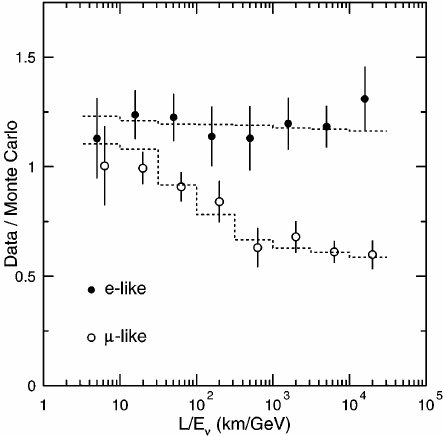
\includegraphics[width=0.7\textwidth]{figures/sk_flux.jpg}

	\caption
	[Ratio of data to Monte Carlo for electron and muon neutrino fluxes 
	measured by the Super Kamiokande experiment as a function of 
	\(\mbox{L} / \mbox{E}_\nu\).]
	{Ratio of data to Monte Carlo for electron and muon neutrino fluxes measured 
	by the Super Kamiokande experiment as a function of 
	\(\mbox{L} / \mbox{E}_\nu\). The Monte Carlo prediction is based on the
	assumption of no oscillations. The muon neutrino flux is consistent with the
	no oscillation prediction at small \(\mbox{L} / \mbox{E}_\nu\), however, for
	large \(\mbox{L} / \mbox{E}_\nu\) a clear deficit is observed. The best fit
	under the assumption of atmospheric (\(\nu_\mu \rightarrow \nu_\tau\))
	oscillations is shown, the best fit parameters are \(\Delta m^2 = 2.2 \times
	10^{-3} \mbox{eV}^2\), and \(\sin^22\theta = 1\). Figure from 
	\cite{Fukuda1998}.}
	\label{fig:sk_flux}

\end{figure}

While it wouldn't pin down the exact cause of the solar neutrino problem, the
Sudbury Neutrino Observatory (SNO) was able to provide unique insight into the 
observed solar neutrino fluxes in 2002. Unlike other water Cerenkov detectors, 
SNO was filled with heavy water, \(\mbox{D}_2\mbox{O}\), instead of its 
lighter isotope. The use of heavy water gives rise to additional neutrino 
interactions which allowed the SNO experiment to distinguish between three 
different interaction modes: charged current (CC), neutral current (NC), and 
elastic scattering (ES). Each mode is sensitive to different parts of the 
solar neutrino flux, including some sensitivity to the muon neutrino and tau 
neutrino fluxes via the NC and ES interactions. Analysis of the data for each 
of the three unique interaction modes lead to a measurement of the flavour 
composition of the solar neutrino flux at earth, while also finding the 
overall neutrino flux at earth to be consistent with the SSM.  Figure 
\ref{fig:sno_flux} shows the composition of the solar neutrino flux as 
measured in the SNO experiment\cite{Ahmad2002}, the flux prediction based on 
the measured rate of NC events is consistent with the predictions of the SSM. 
The composition of solar neutrinos measured in the SNO experiment is not a 
result of simple neutrino oscillations, it also depends on the effect of matter 
on the neutrino propagation in the Sun via the Mikheyev–Smirnov–Wolfenstein 
(MSW) effect. However at the time a number of solutions were still possible: 
MSW conversion, decoherence, neutrino decay, and others\cite{Smirnov:2016xzf}. 

\begin{figure}

	\centering

	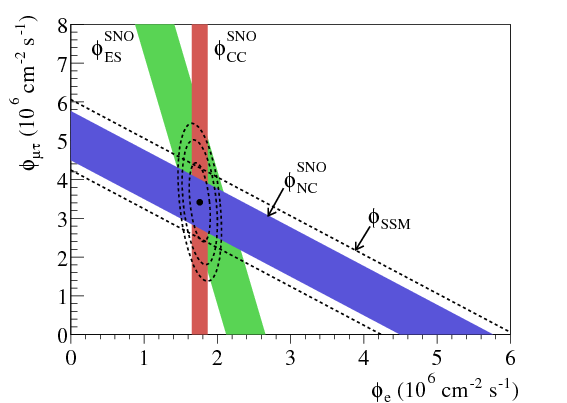
\includegraphics[width=0.8\textwidth]{figures/sno_flux.png}

	\caption
	[Solar neutrino flux composition as measured by the SNO experiment.]
	{Solar neutrino flux composition as measured by the SNO experiment. The
	coloured bands represent the measured flux of charged current (CC),
	neutral current (NC), and elastic scattering (ES) events, including a \(\pm 1
	\sigma\) spread. The central contours represent 68\%, 95\%, and 99\%
	probability contours for the joint \(\phi_e\) and \(\phi_{\mu \tau}\) fit. The
	dashed lines represent the predicted flux of \(^8\mbox{B}\) neutrinos based on 
	the standard solar model. Figure from \cite{Ahmad2002}. }

	\label{fig:sno_flux}

\end{figure}

An \(\mbox{L/E}_\nu\) dependence in the neutrino flux would have to be measured 
in order for neutrino oscillations to be the unique solution to the problem. 
To make this measurement a much shorter neutrino baseline would be needed, and a
detector with good energy resolution. In 2002 the Kamioka Liquid Scintillator 
Anti--neutrino Detector (KamLAND) experiment measured \(\xoverline{\nu_e}\) 
oscillations from a number of nuclear reactors, which produce neutrinos at the 
MeV scale\cite{ Eguchi2003, Araki2005}. Along with an overall deficit of 
neutrino events, they were able to use the high energy resolution of the 
KamLAND detector to measure an \(\mbox{L/E}_\nu\) dependence of the 
\(\xoverline{\nu_e}\) survival probability.  Figure 
\ref{fig:kamland_spectrum}, shows the ratio of the observed neutrino flux with 
the no oscillation predicted flux as a function of \(\mbox{L/E}_\nu\), a clear 
dependence can be seen and this data was enough to prove that neutrino 
oscillations were the only solution to the solar neutrino problem.  

\begin{figure}

	\centering

	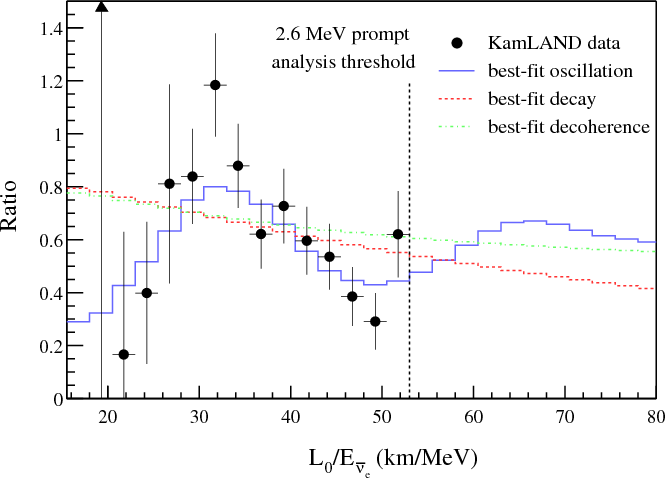
\includegraphics[width=0.8\textwidth]{figures/kamland_spec.png}

	\caption
	[Ratio of observed neutrino flux to the predicted flux in the absence of
	neutrino oscillations in the KamLAND experiment.]
	{Ratio of observed neutrino flux to the predicted flux in the absence of
	neutrino oscillations in the KamLAND experiment as a function of 
	\(\mbox{L/E}_\nu\). The data are fit with three different models: the red 
	dashed line represents the best fit to a neutrino decay model, the green 
	dashed line is for a decoherence model, and the solid blue line represents the 
	best fit of the data to a neutrino oscillation model. The neutrino oscillation
	model, which has a different shape to the other two models, is found to give 
	the best fit to the data. Figure from \cite{Araki2005}.} 

	\label{fig:kamland_spectrum}

\end{figure}

Based on the results of the above experiments, it was assumed that electron and
muon type neutrinos oscillate into tau type neutrinos, which then
went undetected. The first evidence of tau neutrino production in oscillations
wouldn't come until 2010, when the OPERA experiment measured a \(\nu_\tau\) 
candidate in a \(\nu_\mu\) beam. They used similar emulsion detectors to those 
used to discover the \(\nu_\tau\) in DONUT, and a muon neutrino beam on a 730 km 
baseline from CERN to Laboratori Nazionali del Gran Sasso (LNGS). By the end 
of the experiment a total of 10 candidate events have been observed, 6.1 
\(\sigma\) above the expected background\cite{Agafonova2010, Agafonova2018}.

Since the discovery of neutrino oscillations, many more experiments have made
measurements of oscillations and the majority of the parameters of the neutrino
oscillation models have been constrained. Important results of these 
experiments for constraining the parameters of the neutrino oscillation models 
will be highlighted in Section \ref{nu_osc}, along with a theoretical overview 
of neutrino oscillations.

\section{Neutrinos in the Standard Model} \label{nu_sm}

In the standard model neutrinos form part of the left handed fermion doublets
\begin{equation}
	\psi_i = \begin{pmatrix}[1.5] \nu_i \\ l^-_i \end{pmatrix},
\end{equation}
where they are paired with a charged lepton of the same flavour in
CC interactions, and $i$ represents any of the three known generations of 
leptons. Their interactions with other particles in the standard model is
determined by the electroweak (EW) theory, which is derived from the $SU(2)
\times U(1)$ gauge group. The neutrino fields enter into the SM Lagrangian in
the CC and NC interactions:
\begin{align}
	\label{eqn:cc_lag}
	\mathcal{L}^{CC} &= -\frac{g_W}{\sqrt{2}}\; j^{CC}_\alpha(x)\; W^\alpha(x)\; +\; h.c. \\
	\mathcal{L}^{NC} &= -\frac{g_W}{cos\theta_W}\; j^{NC}_\alpha(x)\; Z^\alpha(x)\; +\; h.c.
\end{align}
Here 
\begin{equation}
	\label{eqn:cc_curr}
	j^{CC}_{\alpha}(x) = \sum_{\beta=e,\mu,\tau} \xoverline{\nu_\beta}(x)\;
	\gamma_{\alpha} \; \frac{1}{2} \left(1 - \gamma^5 \right) l_\beta(x)
\end{equation}
is the leptonic charged--current and
\begin{equation}
	j^{NC}_{\alpha}(x) = \frac{1}{2} \sum_{\beta=e,\mu,\tau} \xoverline{\nu_\beta}(x)\;
	\gamma_{\alpha}\; \frac{1}{2} \left(1 - \gamma^5 \right)  \nu_\beta(x)
\end{equation}
is the neutrino neutral--current, $W^\alpha(x)$ and $Z^\alpha(x)$ are the vector
boson fields for the $W^\pm$ and $Z^0$ bosons respectively, $g_W$ is the 
electroweak coupling constant, and $\theta_W$ is the Weinberg angle.

Mass is included in the standard model through the Dirac mass term in the
Lagrangian
\begin{align}
	\mathcal{L}^{D} &= m_D \xoverline{\psi} \psi \nonumber \\
	&= m_D \overline{(\psi_L + \psi_R)}(\psi_L + \psi_R) \nonumber \\ 
	&= m_D(\xoverline{\psi}_L \psi_R + \xoverline{\psi}_R \psi_L)
\end{align}
where $L$ and $R$ represent the left and right handed components of the field.
The lack of right handed neutrino states, therefore, means neutrinos are assumed 
to be massless in the standard model. For massive neutrinos to exists the 
standard model, right handed neutrino fields need to be introduced. In addition, 
it is still not known whether neutrinos are Dirac or Majorana particles, meaning that 
additional Majorana mass terms are possible. A more general neutrino mass term 
including both Dirac and Majorana components is 
\begin{equation}
	\label{eqn:m_dirac_majorana}
	\mathcal{L}^{D+M} = 
	\begin{pmatrix}[1.5] \xoverline{\nu}_L \; \xoverline{\nu}_R \end{pmatrix} 
	\begin{pmatrix}[1.5] m_L \; m_D \\ m_D \; m_R \end{pmatrix} 
	\begin{pmatrix}[1.5] \nu_L \\ \nu_R \end{pmatrix}.
\end{equation}

\section{Neutrino Oscillations} \label{nu_osc}

Neutrino oscillations are a result of quantum mechanical interference between
different massive neutrino eigenstates. Neutrinos are produced in a state of 
definite flavour, \(\alpha = e, \mu, \tau\), in charged current (CC) and 
neutral current (NC) weak interactions, 
\begin{equation}
	W^+ \rightarrow l_\alpha^+ \nu_\alpha, \quad  W^- \rightarrow l^-_\alpha \nu_\alpha, \quad  Z   \rightarrow \nu_\alpha \xoverline{\nu_\alpha}.
\end{equation}
The CC processes are used in neutrino oscillation experiments because
they give information about the initial flavour state of the neutrinos. These
processes are governed by the Lagrangian of the CC leptonic interactions, as in
Equation \ref{eqn:cc_lag}.

Neutrino flavour states, $\nu_\alpha$, can be represented as a superposition of 
neutrino mass eigenstates in any case where the energy and momentum of the 
neutrino is not known with enough precision to determine the neutrino mass. 
The basis transformation takes the form
\begin{equation}
	\label{eqn:mass_sup}
	\nu_\alpha = \sum_{k} U^*_{\alpha k} \nu_k,
\end{equation}
where $\nu_k$ are the neutrino mass eigenstates, and U is a unitary mixing
matrix. 

The representation of neutrino flavour states as a superposition of mass 
eigenstates gives rise to the phenomenon of neutrino oscillations. Consider a 
neutrino produced in a CC weak interaction with flavour \(\alpha\). 
This neutrino flavour state is described by equation \ref{eqn:mass_sup},
where \(U\) is a unitary mixing matrix called the PMNS 
(Pontecorvo, Maki, Nakagawa, and Sakata) matrix. For three flavour mixing the 
PMNS matrix takes the form:
\begin{equation}
	\label{eqn:pmns}
	U = 
	\begin{pmatrix}[2]
		U_{e1} & U_{e2} & U_{e3} \\
		U_{\mu1} & U_{\mu2} & U_{\mu3} \\
		U_{\tau1} & U_{\tau2} & U_{\tau3} \\
	\end{pmatrix}.
\end{equation}

\subsection{Neutrino Oscillations in Vacuum}
In a vacuum, the neutrino mass states are eigenstates of the free particle Hamiltonian
\begin{equation}
	\label{eqn:ham_eig}
	{\cal H} \ket{\nu_k} = E_k \ket{\nu_k},
\end{equation}
with energy
\begin{equation}
	\label{eqn:nu_en}
	E_k = \sqrt{\vb{p}^2 + m_k^2}.
\end{equation}
So the solutions to the time dependent Schrodinger equation are plane waves
\begin{equation}
	\label{eqn:plane_wave}
	\ket{\nu_k(t)} = e^{-iE_kt}\ket{\nu_k}.
\end{equation}
The time evolution of the initial flavour state is:
\begin{equation}
	\label{eqn:flavour_time_mass}
	\ket{\nu_\alpha(t)} = \sum_k U_{\alpha k}^* e^{-iE_kt} \ket{\nu_k}.
\end{equation}

The mass states can be written in terms of the flavour states by inverting
Equation \ref{eqn:mass_sup}:
\begin{equation}
	\label{eqn:flav_sup}
	\ket{\nu_k} = \sum_\alpha U_{\alpha k} \ket{\nu_\alpha}.
\end{equation}
Here, we have used the fact that the states form an orthonormal basis,
\(\braket{\nu_\alpha}{\nu_\beta} = \delta_{\alpha \beta}\), and that the 
transformation matrix is unitary, \(UU^\dagger = \vb{1}\).

Substituting Equation \ref{eqn:flav_sup} into the time evolution of the flavour
state, Equation \ref{eqn:flavour_time_mass}, gives:
\begin{equation}
	\label{eqn:flavour_time_flav}
	\ket{\nu_\alpha(t)} = \sum_{\beta = e, \mu, \tau} \left(\sum_k
	U^*_{\alpha k} e^{-iE_kt} U_{\beta k} \right) \ket{\nu_{\beta}} 
\end{equation}
So as the initial flavour state evolves with time, it becomes a superposition 
of different flavour states; this process is known as neutrino oscillation.
The probability of finding the initial neutrino in flavour state \(\nu_\beta\) 
as a function of time is:
\begin{align}
	\label{eqn:p_osc_u}
	P_{\nu_\alpha \rightarrow \nu_\beta}(t) &= \abs{\braket{\nu_\beta}{\nu_\alpha(t)}}^2 \\
	                               &= \sum_{kj} U^*_{\alpha k} U_{\beta k} U_{\alpha j} U^*_{\beta j} e^{-i(E_k - E_j)t}.
\end{align}

All neutrino oscillation experiments to date operate in a regime where 
\(E \gg m\), in this regime the relativistic energy relation for neutrinos can 
be expanded as \({E_k \simeq E + \frac{m_k^2}{2E}}\), where \(E = \abs{p}\). 
Hence, 
\begin{equation}
	\label{eqn:energy_diff}
	E_k - E_j \simeq \frac{m_k^2 - m_j^2}{2E} = \frac{\Delta m_{kj}^2}{2E}.
\end{equation}
In addition, neutrino oscillation experiments do not measure the neutrino
propagation time \(t\). Instead, they measure the propagation distance, \(L\), 
also known as the baseline. In the ultra--relativistic limit we can approximate 
\({t \simeq L}\) in natural units. As a result, Equation \ref{eqn:p_osc_u} can be
approximated as:
\begin{align}
	\label{eqn:p_osc_u_l}
	P_{\nu_\alpha \rightarrow \nu_\beta}(t) &= \sum_{kj} U^*_{\alpha k} U_{\beta k} U_{\alpha j} U^*_{\beta j} e^{-i\frac{\Delta m^2_{kj}L}{2E}}.
\end{align}

Splitting the sum into its real and imaginary parts emphasises the possibility
of CP--violation in neutrino oscillations. CP--violation occurs if the imaginary
component of the matrix product is none--zero. 
\begin{align}
	\label{eqn:p_osc_im_re}
	P_{\nu_\alpha \rightarrow \nu_\beta}(t) = \delta_{\alpha \beta} 
	&- 4 \sum_{j > k} \operatorname{Re}(U^*_{\alpha k} U_{\beta k} U_{\alpha j} U^*_{\beta j}) \sin^2(\frac{\Delta m^2_{kj} L}{2E}) \nonumber \\
	&\pm 2 \sum_{j > k} \operatorname{Im}(U^*_{\alpha k} U_{\beta k} U_{\alpha j} U^*_{\beta j}) \sin^2(\frac{\Delta m^2_{kj} L}{2E}).
\end{align}
The third term here is responsible for CP violation in neutrino oscillations,
the positive case corresponds to neutrinos and the negative case is for
anti--neutrinos.

The probability of oscillation is, therefore, dependent on properties determined
by nature, in the form of PMNS matrix elements and mass squared differences, and
those which can be chosen by experiments, the distance travelled, L, and the
neutrino energy, E. In a vacuum, the oscillation probability is only dependent 
on the magnitude of the squared mass difference between the neutrino mass
eigenstates. It gives no information about the absolute masses of the 
neutrino eigenstates or their ordering. The question of the absolute
neutrino masses cannot be answered in neutrino oscillation experiments. To get
access to the absolute masses other experiments are required, e.g. direct mass
measurements with tritium beta decay experiments such as 
KATRIN\cite{Aker:2019qfn}.  Neutrino oscillation experiments can give insight 
on the ordering of the neutrino masses, but to understand how the oscillations 
of neutrinos in matter must be considered.

\subsection{Neutrino Oscillations in Matter}
In real neutrino oscillation experiments, neutrinos travel through matter,
whether it be the matter in a star or the earths crust. Neutrinos propagating in
matter are subject to an additional potential due to the interaction of the 
neutrinos with the electrons and nucleons in the medium.  This interaction can 
significantly modify the flavour of the beam relative to oscillations in 
vacuum.

In matter neutrinos can scatter off particles by interacting with either
the charged--current or neutral--current interactions as shown in Figure
\ref{fig:nu_in_matter}. These interactions give rise to additional effective
potentials which the neutrinos experience while they are travelling,
\begin{align}
	V_{CC} &= \sqrt{2} G_F N_e, \\
	V_{NC}^f &= \sqrt{2} G_F N_f g_V^f,
\end{align}
where $G_F$ is the Fermi weak coupling constant, $N_e$ and $N_f$ are the number
densities of electrons and other fermions respectively, and $g_V^f$ is the
vector coupling constant for a given fermion f.
\begin{figure}
	\centering

	\begin{subfigure}[b]{0.49\textwidth}
		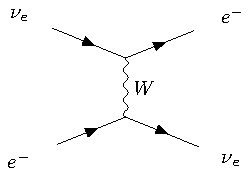
\includegraphics[width=\textwidth]{latex_extras/ne_cc.pdf}
		\caption{Charged current scattering.}
		\label{fig:nu_cc}
	\end{subfigure}
	\hfill
	\begin{subfigure}[b]{0.49\textwidth}
		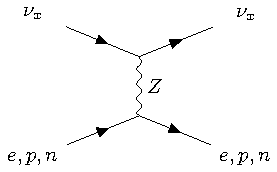
\includegraphics[width=\textwidth]{latex_extras/n_nc.pdf}
		\caption{Neutral current scattering.}
		\label{fig:nu_nc}
	\end{subfigure}

	\caption
	[Feynman diagrams for neutrino scattering in matter.]
	{Feynman diagrams for neutrino scattering in matter.}

	\label{fig:nu_in_matter}
\end{figure}

Neutral--current scattering is independent of neutrino flavour meaning that
the additional potential does not affect oscillations. However, the charged
current potential is only present for $\nu_e$ and, therefore, it will impact the
mass eigenstates by different amounts depending on their relative $\nu_e$
component.

A full description of the effects of matter on neutrino oscillations is beyond
the scope of this thesis, although it is discussed at length in other sources
such as\cite{GiuntiCarlo2007FoNP}. For the purposes of this thesis it is
sufficient to note that the propagation of neutrinos in matter changes the
oscillations probabilities, and this must be taken into account by oscillation
experiments.

One implication of the effects of matter on oscillations is that it introduces
sensitivity to sign of the mass splittings\cite{GiuntiCarlo2007FoNP}, 
allowing experiments to determine the relative ordering of the neutrino 
masses. By considering the pattern of neutrino oscillations in the sun it is 
possible to determine that $\Delta m_{21}^2 > 0$\cite{PhysRevD.98.030001}. 
The sign of the remaining mass splitting, $\Delta m_{32}^2$, remains unknown 
which leaves two possibilities for the ordering of neutrino masses. Normal 
ordering (NO), in which $m_3 > m_2 > m_1$, and inverted ordering (IO), where $m_1 > m_2 
> m_3$, which are depicted in Figure \ref{fig:mass_ordering}. 
\begin{figure}
	\centering
	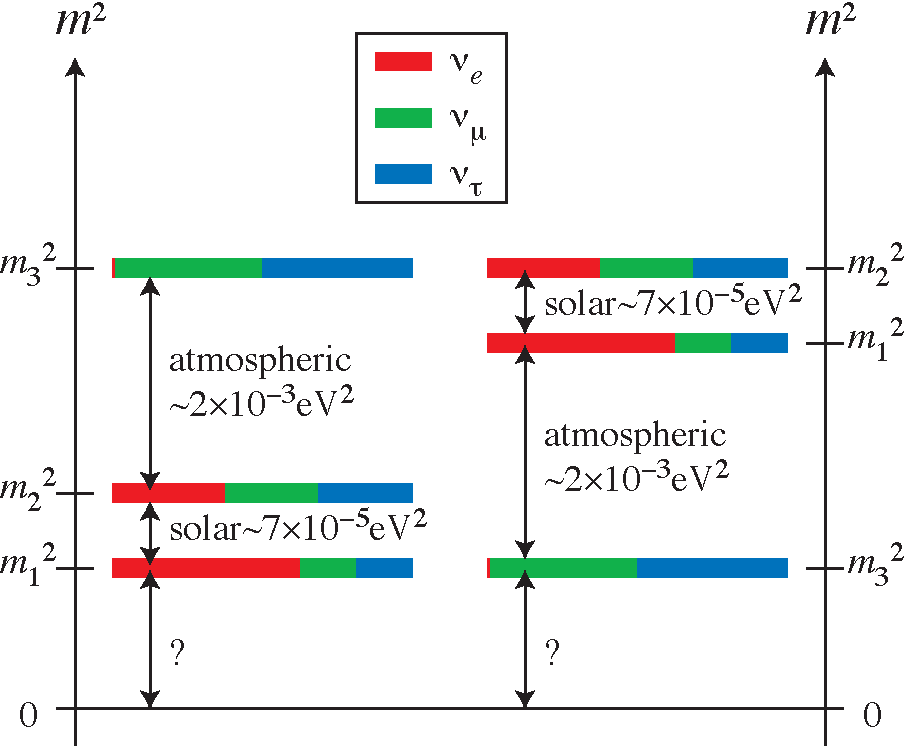
\includegraphics[width=0.7\textwidth]{figures/mass.pdf}
	\caption
	[The two possible neutrino mass orderings: normal and inverted.]
	{The two possible neutrino mass orderings. Left: normal ordering. Right: 
	inverted ordering.  Figure from \cite{SKing}.}
	\label{fig:mass_ordering}
\end{figure}

\newpage
\subsection{Current Knowledge and Open Questions}

At the time of writing the most widely accepted model of neutrino oscillations
involves three neutrino mass eigenstates. In this model, the PMNS matrix is 
often parametrised in terms of three mixing angles \(\theta_{12}\), 
\(\theta_{13}\), and \(\theta_{23}\) and three CP--violating phases 
\dcp{}, \(\alpha_1\), and \(\alpha_2\):
\begin{equation}
	\label{eqn:pmns_expanded}
	U = 
	\underbrace{\begin{pmatrix}[2] 
		c_{12}  & s_{12} & 0 \\
		-s_{12} & c_{12} & 0 \\
		0       & 0      & 1 \\
	\end{pmatrix}}_{\mbox{\small Solar}}
	\underbrace{\begin{pmatrix}[2]
		c_{13}                 & 0 & s_{13}e^{-i\delta_{CP}} \\
		0                      & 1 & 0 \\
		-s_{13}e^{i\delta_{CP}} & 0 & c_{13} \\
	\end{pmatrix}}_{\mbox{\small Cross--mixing}}
	\underbrace{\begin{pmatrix}[2]
		1 & 0       & 0 \\
		0 & c_{23}  & s_{23} \\
		0 & -s_{23} & c_{23} \\
	\end{pmatrix}}_{\mbox{\small Atmospheric}}
	\underbrace{\begin{pmatrix}[2]
		e^{i\frac{\alpha_1}{2}} & 0                       & 0 \\
		0                       & e^{i\frac{\alpha_2}{2}} & 0 \\
		0                       & 0                       & 1 \\
	\end{pmatrix}}_{\mbox{\small Majorana}}.
\end{equation}
Expressing the mixing matrix like this factorises the matrix into its 
components, which are responsible for oscillations in different regimes. 
The first component contains only \(\theta_{12}\) which is dominant in Solar
neutrino oscillations. The third component dominates in the mixing of 
atmospheric neutrinos, and is a function of \(\theta_{23}\). The final, element 
which is significant for neutrino oscillations is the second component, known 
as the cross--mixing matrix or reactor matrix. This component depends on the 
final mixing angle, \(\theta_{13}\) and on one of the CP--violating phases, 
\dcp{}. If \dcp{} is non--zero then U will have complex components in off 
diagonal elements, leading to different probabilities for CP flipped 
oscillations, \(P(\nu_\alpha \rightarrow \nu_\beta) \neq 
P(\xoverline{\nu_\alpha} \rightarrow \xoverline{\nu_\beta})\). Discovery of 
this effect, which is known as CP--violation,  is one of the major goals of 
the next generation of neutrino oscillation experiments.

The final matrix in the factorised version of the PMNS matrix is called the 
Majorana component. The CP--violating phases in this matrix cancel in the 
oscillation probability, and so they can't be measured in neutrino oscillation 
experiments.  In fact, they only lead to physical effects if neutrinos are 
Majorana particles (i.e. if they are there own antiparticle). Other experiments 
are required to determine if neutrinos are Majorana particles, for example, 
neutrinoless double beta decay experiments such as CUORE\cite{Arnaboldi2004}, 
NEXT\cite{Alvarez2012}, and SNO+\cite{Andringa2016}. The question of the 
nature of neutrinos has implications on neutrino mass generation, as mentioned 
in Equation \ref{eqn:m_dirac_majorana}.

A large number of neutrino oscillation measurements have now been made by
solar, reactor, atmospheric, and accelerator neutrino experiments. When combined
the results of these experiments give us our best estimates of neutrino 
oscillation parameters. The current combined results, from the 2019 Nu--Fit
global neutrino oscillation analysis\cite{Esteban:2018azc} including the solar
neutrino data from Super Kamiokande, along with the major contributing 
experiments for each measurements are summarised below. Each measurement is 
given for both the normal hierarchy and the inverted hierarchy.

\subsubsection*{$\boldsymbol{\theta_{12}}$}

The constraints on the solar mixing angle $\theta_{12}$ are dominated by a
combination of data from solar neutrino experiments (e.g. SNO\cite{Ahmad2002}
and Super Kamiokande\cite{PhysRevLett.86.5651}) with data from the KamLAND 
experiment\cite{Araki2005}. The current constraint is,
\begin{align*}
	\sin^2(\theta_{12}) &= 0.310 \mbox{ } \substack{+ 0.013 \\ - 0.012} \quad \mbox{(NO)} \\
	                    &= 0.310 \mbox{ } \substack{+ 0.013 \\ - 0.012} \quad \mbox{(IO)}
\end{align*}

\subsubsection*{$\boldsymbol{\Delta m^2_{21}}$}

The best measurement of $\Delta m^2_{21}$ is also dominated by a combination of
solar neutrino data with the results from KamLAND. The measured value is,
\begin{align*}
	\Delta m^2_{21} &= (7.39 \mbox{ } \substack{+ 0.21 \\ - 0.20}) \times 10^{-5} \mbox{  eV}^2 \quad \mbox{(NO)} \\
	                &= (7.39 \mbox{ } \substack{+ 0.21 \\ - 0.20}) \times 10^{-5} \mbox{  eV}^2 \quad \mbox{(IO)} \\
\end{align*}

\subsubsection*{$\boldsymbol{\theta_{23}}$ and $\boldsymbol{\Delta m^2_{32}}$}

There is a strong correlation between $\theta_{23}$ and $\Delta m^2_{32}$ and,
therefore, their measurements are usually presented as a two--dimensional
contour. Figure \ref{fig:delm_sin23} shows a comparison of the world leading
contours for $\sin^2 (\theta_{23})$--$\Delta m^2_{32}$, with the tightest error
bands coming from long baseline accelerator experiments such as T2K, MINOS, and 
\nova{}\cite{PhysRevD.96.092006, PhysRevLett.112.191801, PhysRevLett.123.151803}. 
The results are dependent on the neutrino mass ordering, based on the Nu--Fit 
global three neutrino oscillation analysis\cite{Esteban:2018azc}, 
\begin{align*}
	|\Delta m^2_{32}| &= (+ 2.525 \mbox{ } \substack{+ 0.033 \\ - 0.031}) \times 10^{-3} \mbox{  eV}^2 \quad \mbox{(NO)} \\
	                  &= (- 2.512 \mbox{ } \substack{+ 0.034 \\ - 0.031}) \times 10^{-3} \mbox{  eV}^2 \quad \mbox{(IO)},
\end{align*}
and 
\begin{align*}
	\sin^2(\theta_{23}) &= 0.582 \mbox{  } \substack{+ 0.015 \\ - 0.019} \quad \mbox{(NO)} \nonumber \\
	                    &= 0.582 \mbox{  } \substack{+ 0.015 \\ - 0.018} \quad \mbox{(IO)}.
\end{align*}

\begin{figure}
	\centering
	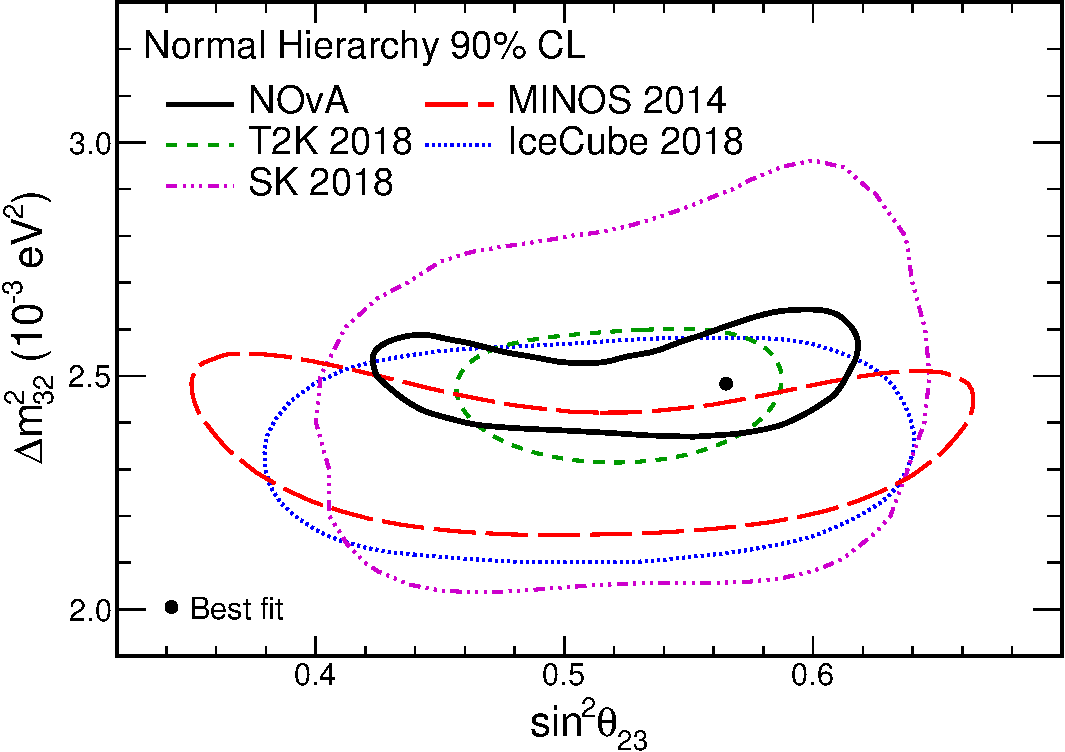
\includegraphics[width=0.9\textwidth]{figures/theta23_msquare.pdf}
	\caption 
	[90\% confidence intervals for $\sin^2 (\theta_{23})$--$\Delta m^2_{32}$.]
	{The 90\% confidence region contours for 
	$\sin^2 (\theta_{23})$--$\Delta m^2_{32}$ from a number of the leading 
	neutrino oscillation experiments\cite{PhysRevD.96.092006, PhysRevLett.112.191801, PhysRevLett.123.151803}. 
	The best fit point for the \nova{} experiment is shown as a black dot.  
	Figure from \cite{PhysRevLett.123.151803}.}
	\label{fig:delm_sin23}
\end{figure}

\subsubsection*{$\boldsymbol{\theta_{13}}$}
Reactor neutrino experiments such as Daya Bay\cite{An:2012eh}, Double 
Chooz\cite{Abe:2013sxa}, and RENO\cite{Ahn:2012nd} have made precise
measurements of $\theta_{13}$, as well as some long baseline oscillation 
experiments, such as T2K and \nova. The Nu--Fit three neutrino global fit to 
the reactor data gives,
\begin{align*}
	\sin^2 \theta_{13} &= 0.02240 \substack{+ 0.00065 \\ - 0.00066} \quad \mbox{(NO)} \\ .
	                   &= 0.02263 \substack{+ 0.00065 \\ - 0.00066} \quad \mbox{(IO)}  
\end{align*}

\subsubsection*{Mass Ordering}
The long baseline oscillation experiments T2K and \nova have both shown a
preference for normal mass 
ordering\cite{PhysRevD.96.092006,PhysRevLett.123.151803}. When these results are
combined in the Nu--Fit three--neutrino oscillation analysis, inverted 
ordering is currently disfavoured with a $\Delta \chi^2 = 9.3$.

\subsubsection*{$\boldsymbol{\delta_{CP}}$}
While there are no accurate measurements of \dcp{} there are some hints that it
may be none--zero from long baseline accelerator neutrino experiments T2K and
\nova{}. These limits are based on joint fits to four data samples: electron
neutrino appearance, electron anti--neutrino appearance, muon neutrino
disappearance, and muon anti--neutrino disappearance.

The T2K experiment's joint fit shows an excess of electron neutrino events and 
a deficit of anti--electron neutrino events when compared to the predictions 
for \(\delta_{CP} = 0\). This results in a preference for negative values of 
\dcp{} with a \(3\sigma\) confidence interval of \([-3.41, -0.03]\) in the 
case of normal neutrino mass ordering. The results of the T2K fit are shown 
in Figure \ref{fig:t2k_cp}\cite{Abe2019}.

\begin{figure}
	\centering
	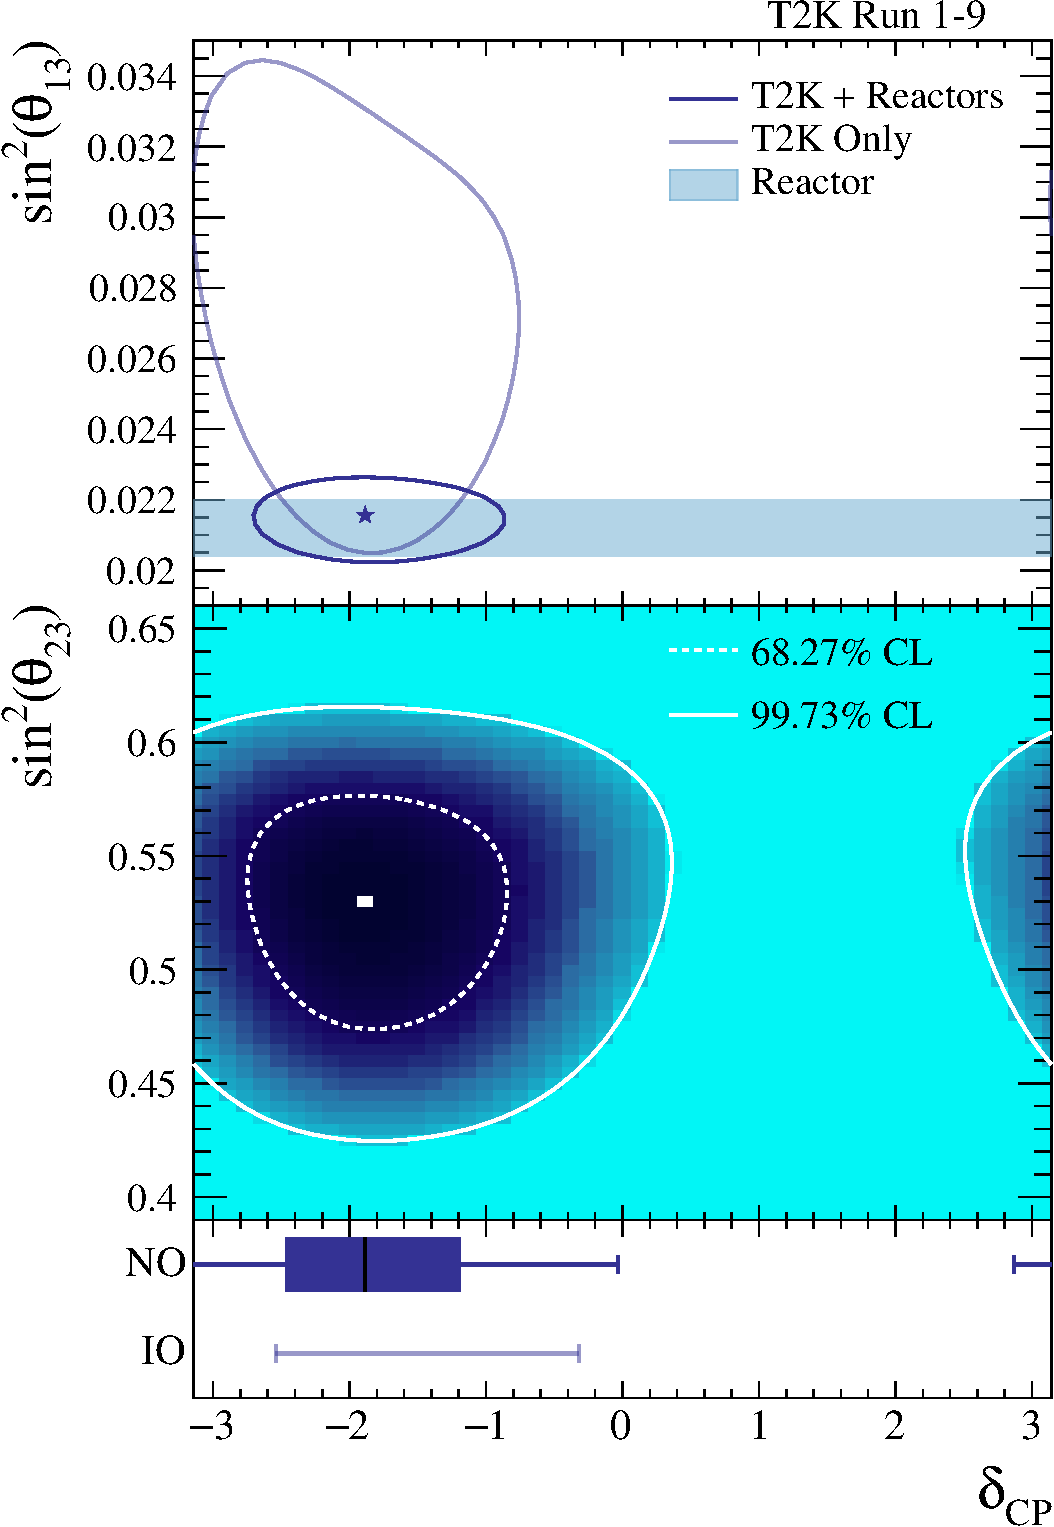
\includegraphics[height=0.6\textheight]{figures/t2k_cp.pdf}
	\caption
	[Confidence intervals for \dcp{} from the T2K experiment.]
	{Confidence intervals for \dcp{} from the T2K experiment. Figure from 
	\cite{Abe2019}. 
	Top: 68.27\% confidence level contours for \dcp{} versus $\sin^2\theta_{13}$ 
	under the assumption of normal ordering. \\
	Middle : Confidence intervals at the 68.27\% and 99.73\% confidence level for 
	\dcp{} versus $sin^2\theta_{23}$ from a fit to T2K and reactor data under the 
	assumption of normal ordering. \\
	Bottom: Confidence intervals for \dcp{} from a fit to T2K and reactor data for 
	both the normal and inverted orderings. The vertical line in the shaded box 
	shows the best-fit value of \dcp{}, the shaded box shows the 68.27\% 
	confidence interval, and the error bar shows the 99.73\% confidence interval. 
	}
	\label{fig:t2k_cp}
\end{figure}

The \nova{} experiment has also performed joint fits to neutrino and
anti--neutrino oscillation data, the results of the fit are shown in Fig.
\ref{fig:nova_cp}. As with T2K the normal mass ordering is preferred, however
for \nova{} the full range of \dcp{} is covered at $3\sigma$ highlighting the 
need for further study of CP--violation in neutrino 
oscillations\cite{PhysRevLett.123.151803}.

\begin{figure}
	\centering
	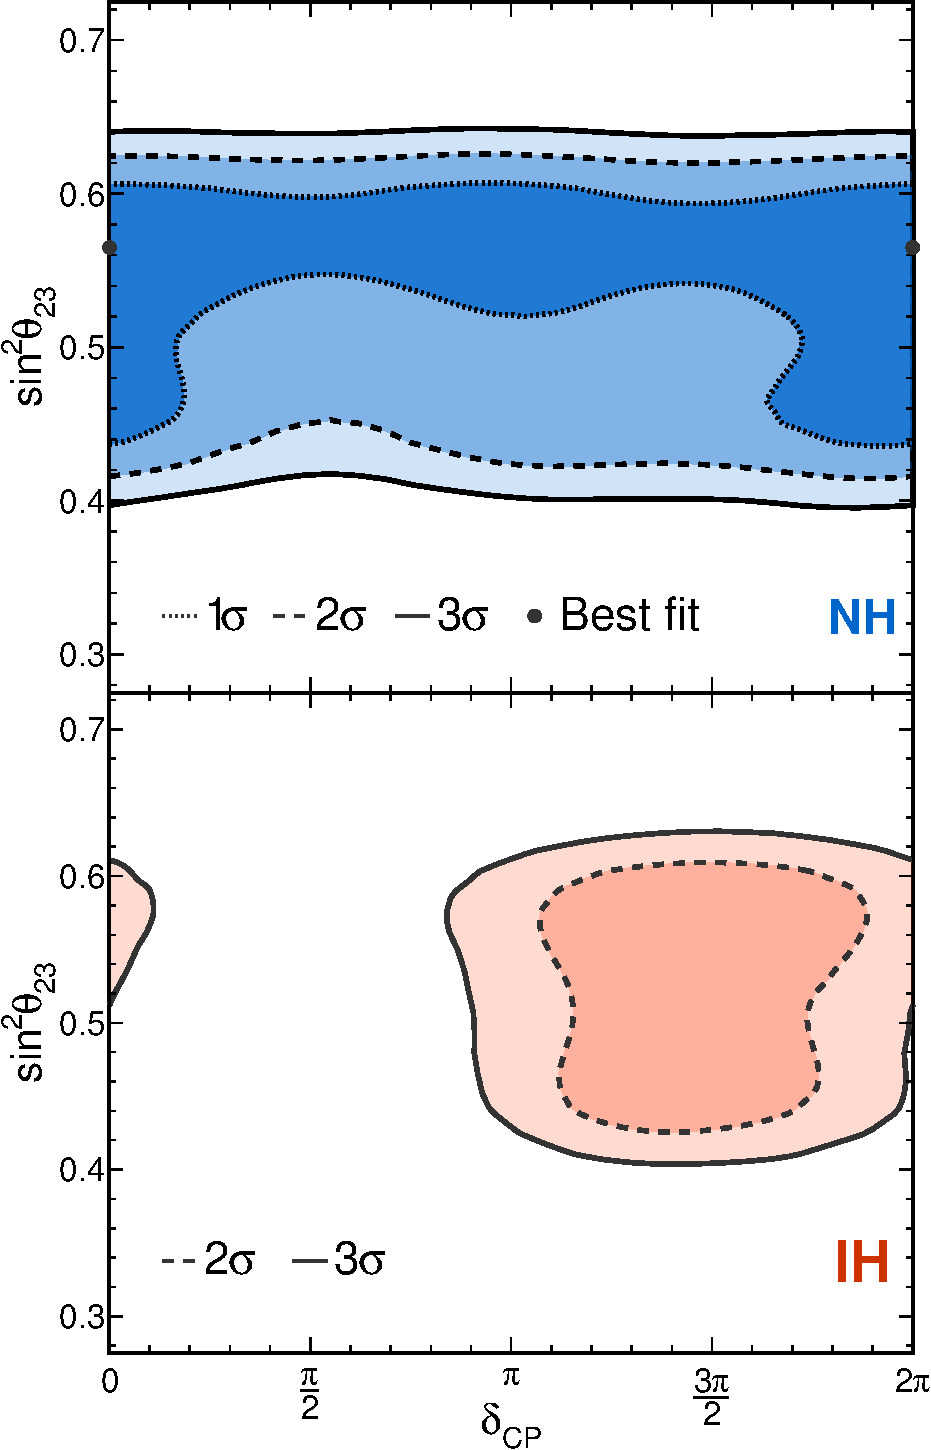
\includegraphics[height=0.7\textheight]{figures/nova_dcp.pdf}
	\caption
	[Confidence intervals for \dcp{} from the \nova{} experiment.]
	{Confidence intervals for \dcp{} from the \nova{} experiment. Figure from 
	\cite{PhysRevLett.123.151803}. \\
	Top: Confidence interval for \dcp{} versus $\sin^2\theta_{23}$ under the
	assumption of normal ordering.\\
	Bottom: Confidence interval for \dcp{} versus $\sin^2\theta_{23}$ under the
	assumption of inverted ordering.\\
	}
	\label{fig:nova_cp}
\end{figure}

\section{Neutrino Interactions} \label{nu_prod}

To perform a neutrino oscillation experiment the composition of the beam needs
to be measured, and the change in beam composition as a function of energy and
distance travelled is analysed. In practice, this relies on measuring
neutrino events and categorising them by flavour in order to compare the
measurement to prediction. However, because we only see the neutrinos that
interact, we are actually seeing the results of a convolution of the neutrino
beam composition with the neutrino interaction cross section. Therefore, it is
important to understand neutrino interaction cross sections to make accurate 
oscillation predictions.

Broadly speaking there are two major types of neutrino interactions:
charged--current (CC) and neutral--current (NC). CC interactions are usually 
used in oscillation experiments because they are the only type of interaction 
which allows the initial flavour of the neutrino to be determined. Some 
NC interactions, e.g. scattering from an electron, produce high energy leptons 
in the detector and, therefore, form an irreducible background which must 
be modelled as part of the experiments simulation.

The types of charged--current interactions available are further split into 
three main categories.

\subsubsection*{Quasi--elastic (QE)}
A neutrino elastically scatters off an individual nucleon. Depending on the
energy transfer, the nucleon may be liberated from the nucleus.
\subsubsection*{Resonance (RES)}
A neutrino excites the target nucleon into a resonance, which then decays
resulting in the possibility of mesons in the final state.
\subsubsection*{Deep Inelastic Scattering (DIS)}
The neutrino has enough energy to resolve the individual quarks within the
target nucleon, liberating the quark and resulting in a hadronic final state.

\bigskip
\noindent
The cross sections for these processes vary as a function of neutrino energy,
and they are each dominant in different energy regimes. Predictions and 
measurements of the charged--current cross section for $\nu_\mu$ are shown in 
Figure \ref{fig:numu_xsec}, the three main components of the cross section are 
shown and the energy range relevant for DUNE is 
highlighted\cite{Formaggio:2013kya}. Within the energy range of the DUNE beam 
all three of the major neutrino cross section components have a region in 
which they dominate, this means that understanding each of these cross 
sections is crucial for any neutrino oscillation measurement in DUNE. 

\begin{figure}
	\centering
	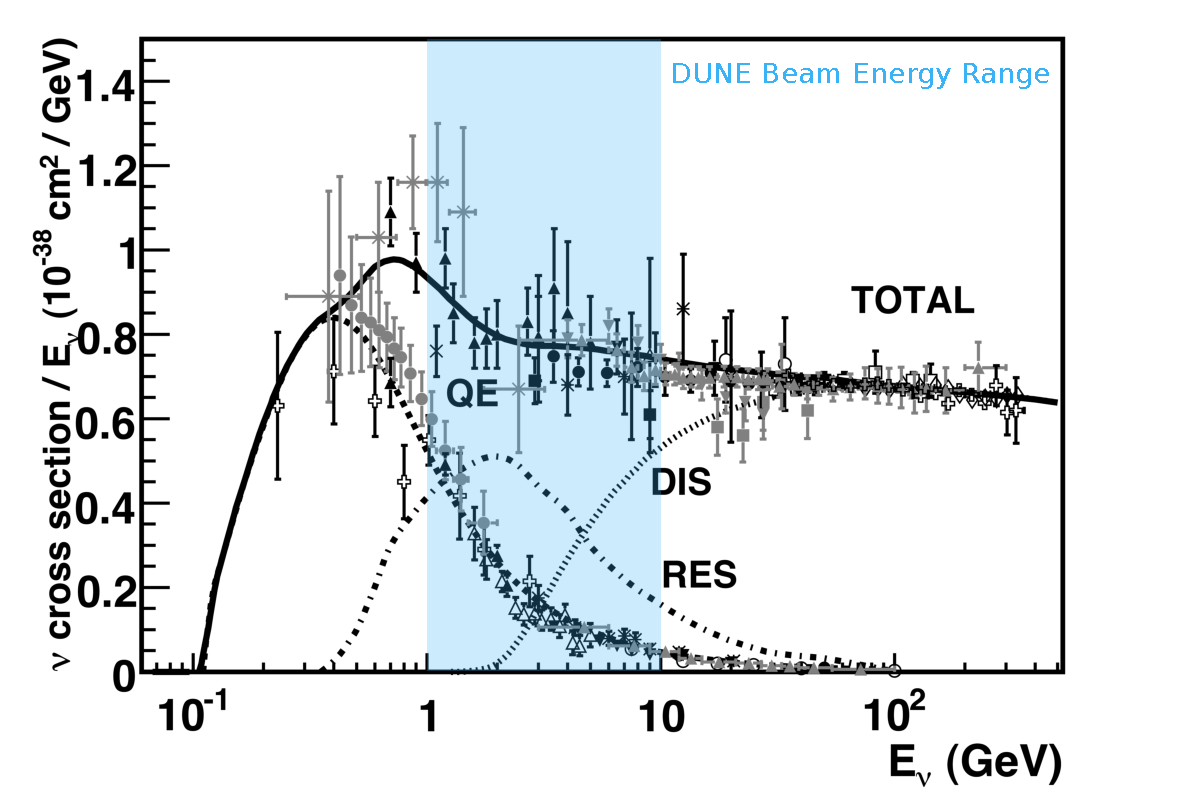
\includegraphics[width=\textwidth]{figures/numu_xsec.pdf}
	\caption
	[Muon neutrino cross section as a function of energy.]
	{Muon neutrino cross section as a function of neutrino energy. The light blue
	region represents the region of interest for the DUNE neutrino beam. Original 
	figure from \cite{Formaggio:2013kya}.}
	\label{fig:numu_xsec}
\end{figure}

The array of interaction modes available in DUNE means that there are many
particles which can be produced in the final state; understanding 
the composition of the final state is essential to the neutrino oscillation 
analysis. Part of this thesis, Chapter \ref{ch:chargeid}, looks at
the identification of charge deposits in a liquid argon TPC. The results 
provide input in the analysis of \protodune{} data, and the methods used could 
be adapted and developed for application in DUNE. 

\section{Supernova Neutrinos} \label{nu_sn}

Supernovae are extremely violent explosions, which are undergone by certain 
types of stars at the end of their life. These explosions can emit on the 
order of $10^{46}$ Joule of energy, and in certain cases, known as 
core--collapse supernovae, about 99\% of this energy is carried away by 
neutrinos.  Measurements of these neutrinos can provide insight into the 
mechanism involved in supernova bursts, as well as the study of neutrino 
masses\cite{GiuntiCarlo2007FoNP}.  

\subsection{Core--collapse Supernova Dynamics}

Core--collapse supernovae occur in stars with masses of around 10--60 solar 
masses. These stars will have undergone all stages of nuclear fusion during
their life, but since iron is the most tightly bound nucleus there is no fuel 
left to burn after it has been produced. At this stage the iron core of the
star, which has a mass of around 1 solar mass, begins to collapse as the
pressure produced by nuclear fusion is no longer enough to counter the force of
gravity. 

During the collapse of the core electron neutrinos are produced through
electron capture on both nuclei and free protons.
\begin{align}
	e^- + N(Z, A) &\rightarrow N(Z - 1, A) + \nu_e \\
	e^- + p &\rightarrow n + \nu_e
\end{align}
At first, the mean free path of these neutrinos is much longer than the size of
the core and the neutrinos leave the core carrying away their energy. This phase
of the collapse is known as the infall phase, it lasts on the order of 10ms and
releases neutrinos with energies of around 12--16 MeV.

Once the density of the core increases beyond around 
$3\times10^{11} \mbox{g cm}^{-3}$ neutrinos become trapped in the core, as the 
cross section for coherent scattering becomes large enough to prevent neutrinos
from passing through the core. Neutrinos are still being produced by capture 
processes at this point, but they are unable to leave the core.

The core--collapse comes to a sudden halt about 1 second after it began when the
density of the inner core reaches that of nuclear matter. At this stage, the 
core settles into equilibrium as a proto--neutron star while a shock--wave 
caused by this sudden halt propagates out through the layers of the star. 
Behind the shock, neutrino production is accelerated as nuclei are dissociated 
and the free protons capture electrons. Neutrinos begin to build--up behind the 
opaque shock. A few milliseconds after the bounce, the shock reaches a region of
low enough density and becomes transparent, releasing the build--up of neutrinos
in just a few milliseconds, this is known as the neutronisation burst.

One aspect of supernova dynamics which is still under debate is the so--called
revival of the shock. As the shock dissipates through nucleon
dissociation and neutrino emission it becomes weakened and eventually stalls
around 100 ms after the initial bounce. At this time, known as the accretion
phase, matter falls onto the collapsed core. If the shock cannot be revived a
supernova will not occur. It is thought that neutrino flux produced in the 
proto--neutron star is able to revive the shock but the precise mechanics of 
this revival are still under debate. Studies have shown that the impact of 
spherically asymmetries might play an important role in allowing the burst to 
take place\cite{Tamborra:2014aua}. 

After the neutronisation burst the main remaining source of neutrino production
comes from the proto--neutron star. Neutrinos of all flavours are produced in
the core at a temperature of around 40 MeV. The release of neutrinos at this
stage, known as the neutrino cooling phase, is significantly slower than that 
of the neutronisation burst and can last tens of seconds. During this phase, 
much like photons within a star, the neutrinos are mostly contained within the 
opaque environment of the proto--neutron star. They can only escape if they 
travel far enough from the core to a region where the opacity is sufficiently 
low. This region is called the neutrinosphere, it is different for neutrinos 
of different flavours, and for neutrinos and anti--neutrinos. The difference in
the neutrinosphere for each flavour result in different energy distributions 
for each neutrino type, owing to the relative temperature of the star at the 
radius of the neutrinosphere,
\begin{align}
	\langle E_{\nu_e} \rangle &\approx 10 \mbox{MeV} \\
	\langle E_{\xoverline{\nu_e}} \rangle &\approx 15 \mbox{MeV} \\
	\langle E_{\nu_x} \rangle &\approx 20 \mbox{MeV}
\end{align}
where $\nu_x \in \left[\nu_\mu, \xoverline{\nu_\mu}, \nu_\tau, \xoverline{\nu_\tau}\right]$.

\subsection{SN1987A}

The first, and only, experimental observation of neutrinos from a supernova
burst occurred in 1987. A small number of low--energy neutrino events where
detected in coincidence with a supernova burst from the Large Magellanic Cloud,
referred to as SN1987A. Three neutrino detectors reported an excess of low
energy events in coincidence with the supernova: Kamiokande--II, IMB, and 
Baksan. These events are primarily produced by two types of interaction, inverse
beta decay (IBD),
\begin{equation}
	n + \nu_e \rightarrow p + e^+,
\end{equation}
and elastic scattering,
\begin{equation}
	\nu_e + e^- \rightarrow \nu_e + e^-.
\end{equation}
For supernova neutrinos, the inverse beta decay cross section is significantly 
higher than that of elastic scattering, therefore, most events are likely to be
due to inverse beta decay.

\subsubsection{Kamiokande--II}
Kamiokande--II was a water Cerenkov detector containing 2.1 kt of water. A
significant increase in the rate of electron events with respect to background
was observed in a 10 second window which is coincident with 
SN1987A\cite{Hirata:1987hu}. Around 12 events were observed, their time sequence
and amplitudes are shown in Figure \ref{fig:kami_1987}. Unfortunately, due to 
an inaccurate detector clock, the absolute time of these events is only 
accurate to about one minute and, therefore, a time coincidence check with the 
other neutrino observations cannot be made.

\begin{figure}
	\centering
	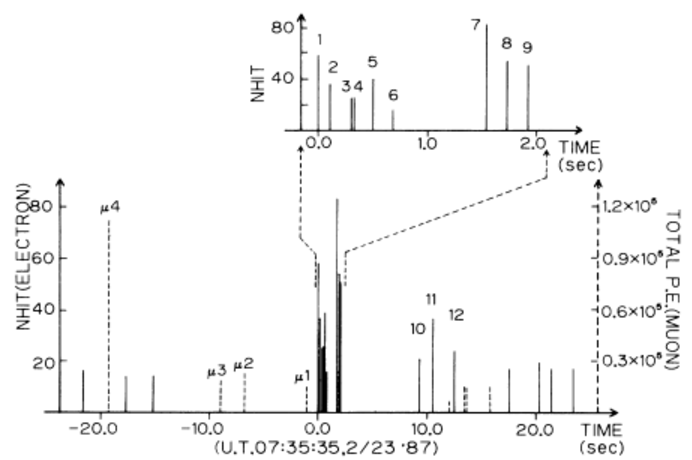
\includegraphics{figures/kami_1987.pdf}
	\caption
	[Measured supernova neutrino events from SN1987A in Kamiokande--II.]
	{Measured time of supernova neutrino events from SN1987A in Kamiokande--II. 
	Electron events are plotted as solid vertical lines, where the height of the 
	line represents the amplitude of the event in terms of number of PMT hits. 
	Muons are represented as dashed vertical lines, and the height of the line 
	represents the total number of measured photo--electrons. A clear excess of 
	electron events can be seen around the centre, this region is expanded above 
	the main axis of the figure. The supernova neutrino candidates are labelled
	with a number above the solid vertical line. Figure from 
	\cite{Hirata:1987hu}.}
	\label{fig:kami_1987}
\end{figure}

\subsubsection{IMB}
IMB was another water Cerekov detector, with a fiducial mass of 3.3 kt. They
observed eight neutrino candidate events with energies in the range of 20--40
MeV within a six second window, the background rate was estimated to be around 2
events per day\cite{PhysRevLett.58.1494}.

\subsubsection{Baksan}
Unlike Kamiokande--II and IMB, the Baksan detector was a segmented liquid
scintillator detector with a total mass of around 330 tons, however only a
limited fiducial mass of around 200 tons was used for the supernova neutrino
measurements. No excess above background could be observed by Baksan
in isolation, however, when assisted by input from Kamiokande--II and IMB, a
cluster of 5 events within a 10s window was observed which coincided with the
measurements from IMB\cite{Loredo:2001rx}.

\bigskip
\noindent
Since SN1987A significant progress has been made for both experimental and
theoretical aspects of neutrino physics. Progress has been made in modelling
supernova explosions, and the impact of neutrino oscillations on the supernova
environment have been considered\cite{Mirizzi:2015eza}. The current and next 
generation of neutrino experiments expect to measure thousands of neutrino 
events for a galactic supernova instead of tens. The flux of neutrinos at earth
has three components $\nu_e$, $\xoverline{\nu_e}$, and $\nu_x$, the predicted 
energy spectra of each component is shown in Figure \ref{fig:sn_spec}.  
Measuring the spectrum and time structure of a supernova neutrino burst could 
provide insights into the dynamics of supernovae, as well as neutrino physics.

\begin{figure}
	\centering
	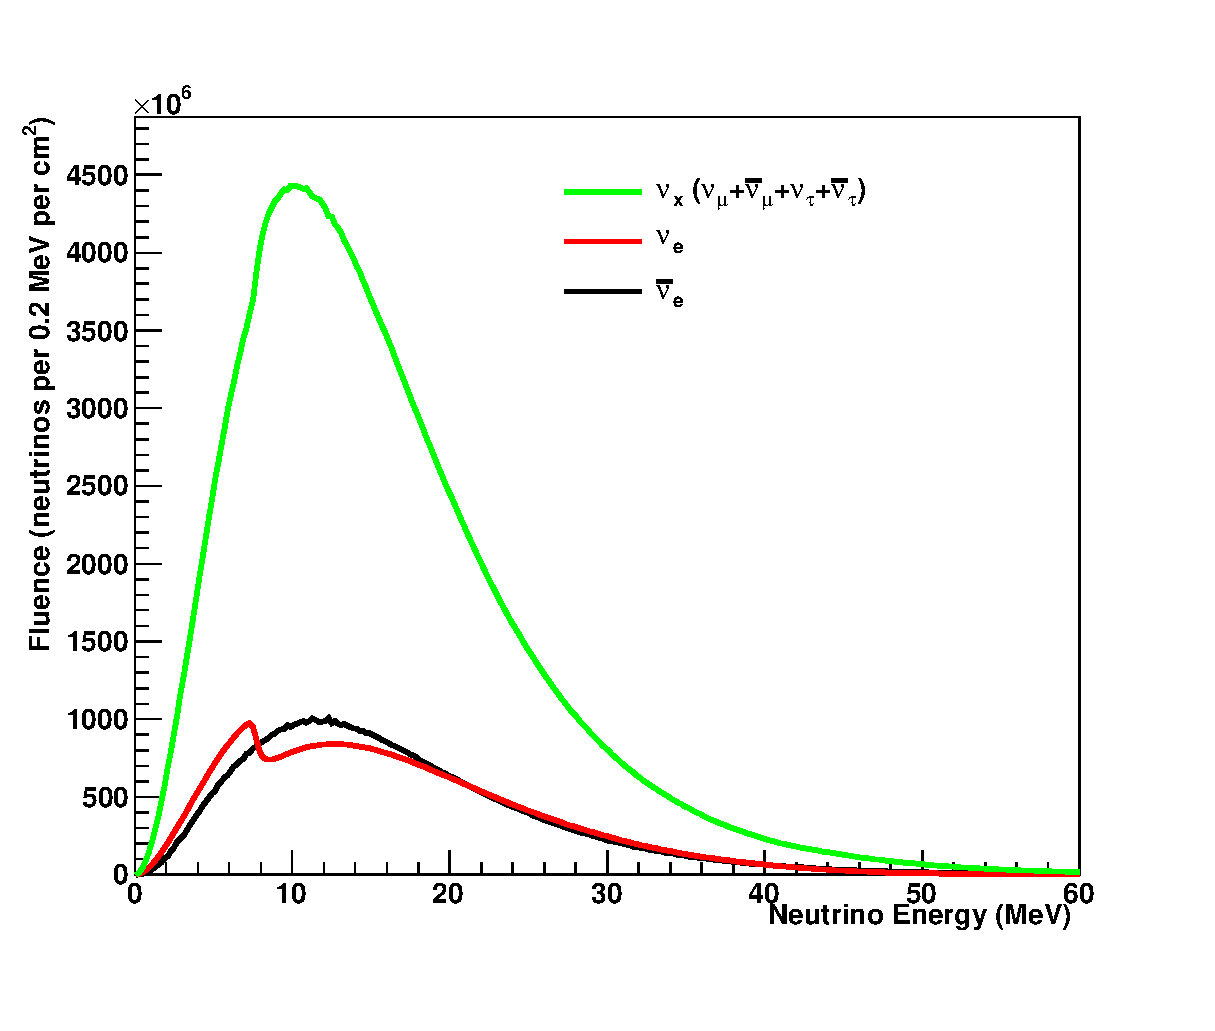
\includegraphics[width=\textwidth]{figures/supernova_spectrum_production.eps}
	\caption
	[Supernova neutrino flux at earth as a function of neutrino energy.]
	{Supernova neutrino flux at earth as a function of neutrino energy. The
	neutrino flux is split into three components, $\nu_e$, $\xoverline{\nu_e}$, 
	and $\nu_x$, which are plotted in red, black, and green respectively. Figure 
	from \cite{Scholberg:2012id}.}
	\label{fig:sn_spec}
\end{figure}

\subsection{Supernova Neutrino Prospects in DUNE}

The current world leading supernova neutrino detector is Super--Kamiokande which
expects to measure around 8000 events for a supernova at 10 
kpc\cite{Abe:2016waf}. As with Kamiokande--II, these events would primarily be
produced via inverse beta decay interactions on the protons within the water.
As such Super--Kamiokande is mostly sensitive to the $\xoverline{\nu_e}$ 
component of the supernova neutrino flux. This is common amongst all water 
Cerenkov and scintillator based detectors and, therefore, the majority of the 
current landscape of supernova neutrino detectors. The large charged--current 
cross section for $\nu_e$ on argon, therefore, makes DUNE a highly complementary 
detector to the other major supernova neutrino detectors, and DUNE offers a 
unique sensitivity to the neutronisation burst, which is primarily made up of 
$\nu_e$.  

\subsubsection{Supernova Neutrino Interactions in Liquid Argon}

Liquid argon should bring a strong sensitivity to the $\nu_e$ component of a
supernova neutrino burst, via the charged--current absorption of $\nu_e$ on
$^{40}\mbox{Ar}$,
\begin{equation}
	\nu_e + ^{40}\mbox{Ar} \rightarrow e^- + ^{40}\mbox{K}^*.
\end{equation}
This interaction leaves an $e^-$ and an excited $K$ in the final state. In 
addition there are charged--current $\xoverline{\nu_e}$ interactions with argon, 
and elastic scattering interactions with electrons, which are available to
neutrinos of all flavours. The dominant cross sections in liquid argon as a 
function of energy are shown in Figure \ref{fig:sn_xsec}\cite{Abi:2020evt}.

\begin{figure}
	\centering
	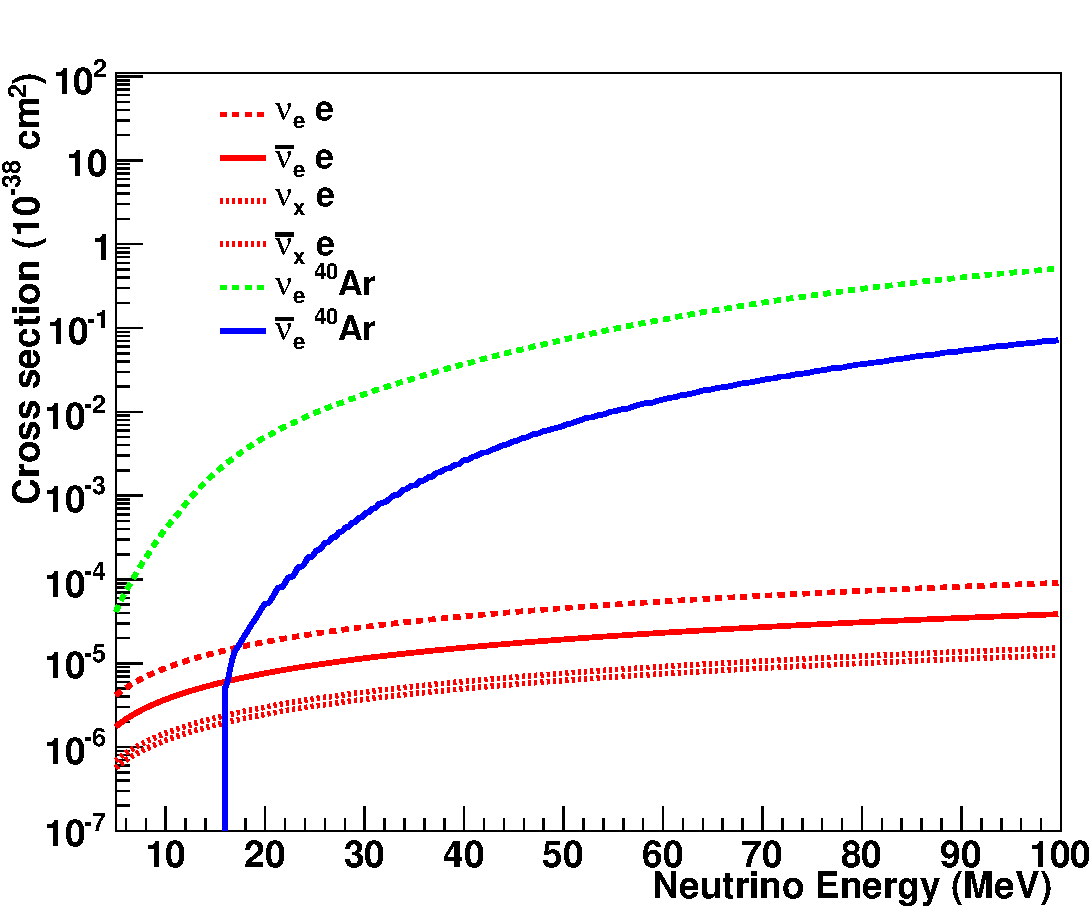
\includegraphics[width=\textwidth]{figures/sn_xsec.pdf}
	\caption
	[Supernova neutrino cross sections as a function of neutrino energy in liquid 
	argon.]
	{Supernova neutrino cross sections as a function of neutrino energy in liquid 
	argon, in the energy regime relevant for supernova neutrinos. Figure from 
	\cite{Abi:2020evt}.}
	\label{fig:sn_xsec}
\end{figure}

\subsubsection{Supernova Neutrino Events in DUNE}

For a 10 kpc supernova DUNE expects to observe roughly 3000 neutrino events,
over a period of around 10 seconds. In DUNE this will show up as a sudden
increase in the rate of low--energy electron events in the detector. Figure 
\ref{fig:sn_nus} shows the predicted time structure and energy spectrum for a 
simulated supernova event in DUNE\cite{Abi:2020evt}. The details of the rate 
and energy of these events as a function of time can hold potential insights 
into both neutrino physics and the dynamics of supernova bursts. 

\begin{figure}
	\centering
	\begin{subfigure}[b]{\textwidth}
		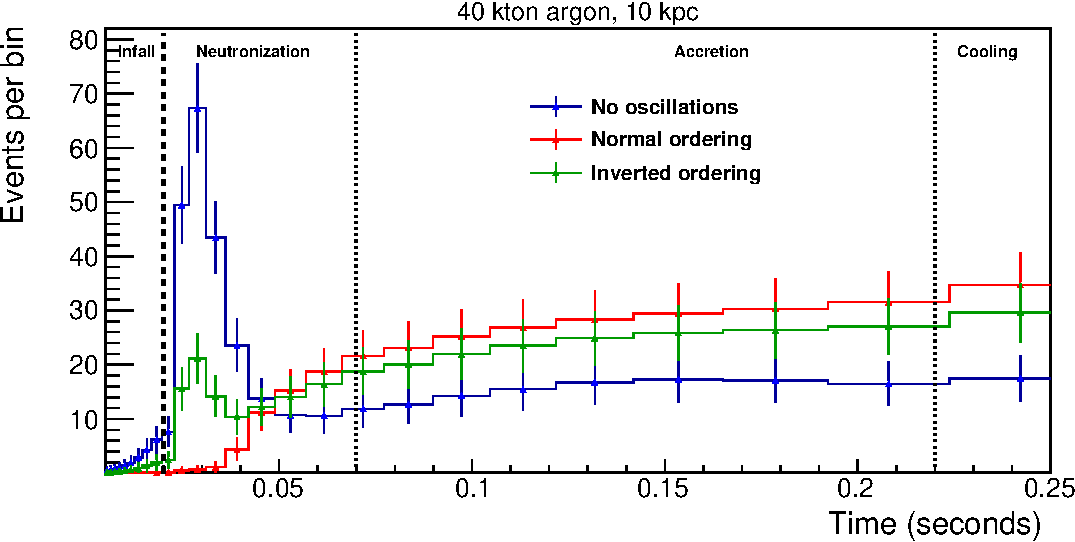
\includegraphics[width=\textwidth]{figures/sn_time.pdf}
		\caption {Observed event rate for the first 0.25 seconds of the supernova
		neutrino burst. The predictions under the assumption of no oscillations, 
		normal neutrino mass ordering, and inverted neutrino mass ordering are shown 
		in blue, red, and green respectively. Figure from \cite{Abi:2020evt}.}
		\label{fig:sn_time}
	\end{subfigure}
	\begin{subfigure}[b]{\textwidth}
		\centering
		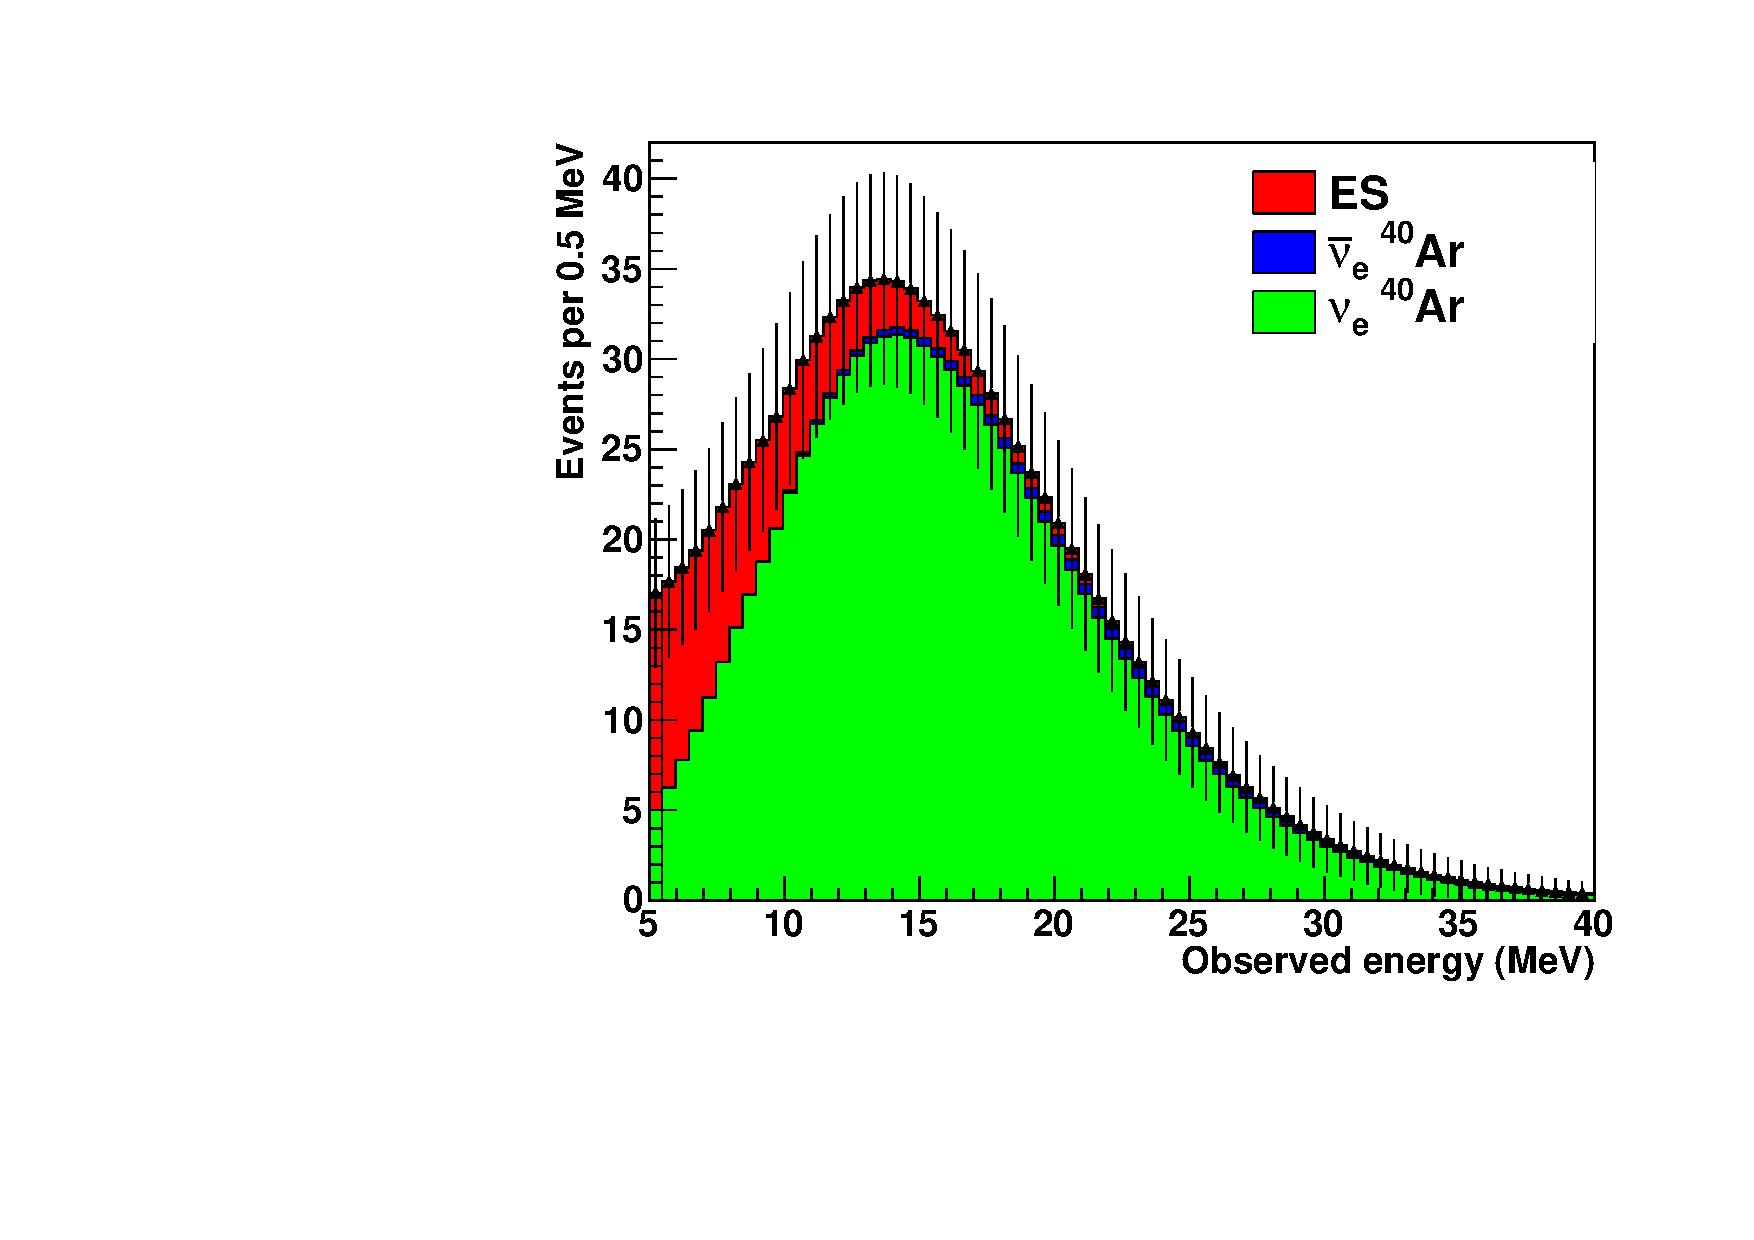
\includegraphics[width=0.9\textwidth]{figures/sn_energy.pdf}
		\caption {Observed supernova neutrino energy spectra for the full supernova
		neutrino burst. The contributions from elastic scattering,
		$\xoverline{\nu_e}$, and $\nu_e$ events are shown in red, blue, and green
		respectively. Figure from \cite{Acciarri:2015uup}.}
		\label{fig:sn_energy}
	\end{subfigure}
	\caption
	[Predicted supernova neutrino event rate and energy spectra for a 10 kpc
	core collapse supernova measured by DUNE.]
	{Predicted supernova neutrino event rate and energy spectra for a 10 kpc
	core collapse supernova measured by DUNE.}
	\label{fig:sn_nus}
\end{figure}

Detecting and reconstructing tens of MeV electrons is necessary to study 
supernova neutrinos, as can be seen from the observed energy spectrum for 
supernova neutrinos in Figure \ref{fig:sn_nus}. There are significant 
challenges involved in this measurement from the detection of low energy 
activity, as well as the impacts of the ionisation geometry of tens of MeV on 
reconstruction.  Effectively reconstructing electrons in the tens of MeV range 
is essential to improving our understanding of supernova neutrinos in DUNE. 
This is one of the subjects of this thesis, and is discussed in chapter 
\ref{ch:michel} using the case of Michel electrons in \protodune{} to 
benchmark the performance of low energy electron reconstruction in liquid 
argon time projection chambers.

\chapter{\label{ch:protodune}The ProtoDUNE--SP Experiment} 

\minitoc

\protodune{} is one of two prototypes for the DUNE Far Detector modules, which 
has been operating at the Neutrino Platform at CERN since the summer of 2018. 
The experiment collected data from a charged particle beam for approximately 3 
months before Long Shutdown 2 of the Large Hadron Collider (LHC). Since then, a 
programme of cosmic--ray data collection has been ongoing.

This chapter will outline the technical details of the \protodune{} experiment.
Section \ref{sec:pdsp_dune} will outline the role of \protodune{} in the context
of the DUNE experiment. This will be followed by a discussion of the main
elements of the \protodune{} detector systems and the H4 beamline, in Sections 
\ref{sec:pdsp_detector} and \ref{sec:h4} respectively. The tagging of 
cosmic--ray muons for calibration is done by the Cosmic--Ray Tagger (CRT), 
which will be discussed in Section \ref{sec:pdsp_cosmic}. Sections 
\ref{sec:simulation} and \ref{sec:reconstruction} will then discuss the 
simulation and reconstruction of \protodune{} data. Finally Section 
\ref{sec:pdsp_om} will cover details of the online monitoring system in 
\protodune{}. During my time at CERN I was the primary developer and expert on
the \protodune{} online monitoring system. The development and maintenance of 
this system represents a significant body of work over a 12 month period, as 
well as ongoing maintenance work throughout the following 2 years.

\section{\protodune{} in the Context of DUNE} \label{sec:pdsp_dune}

\begin{figure}

	\centering

	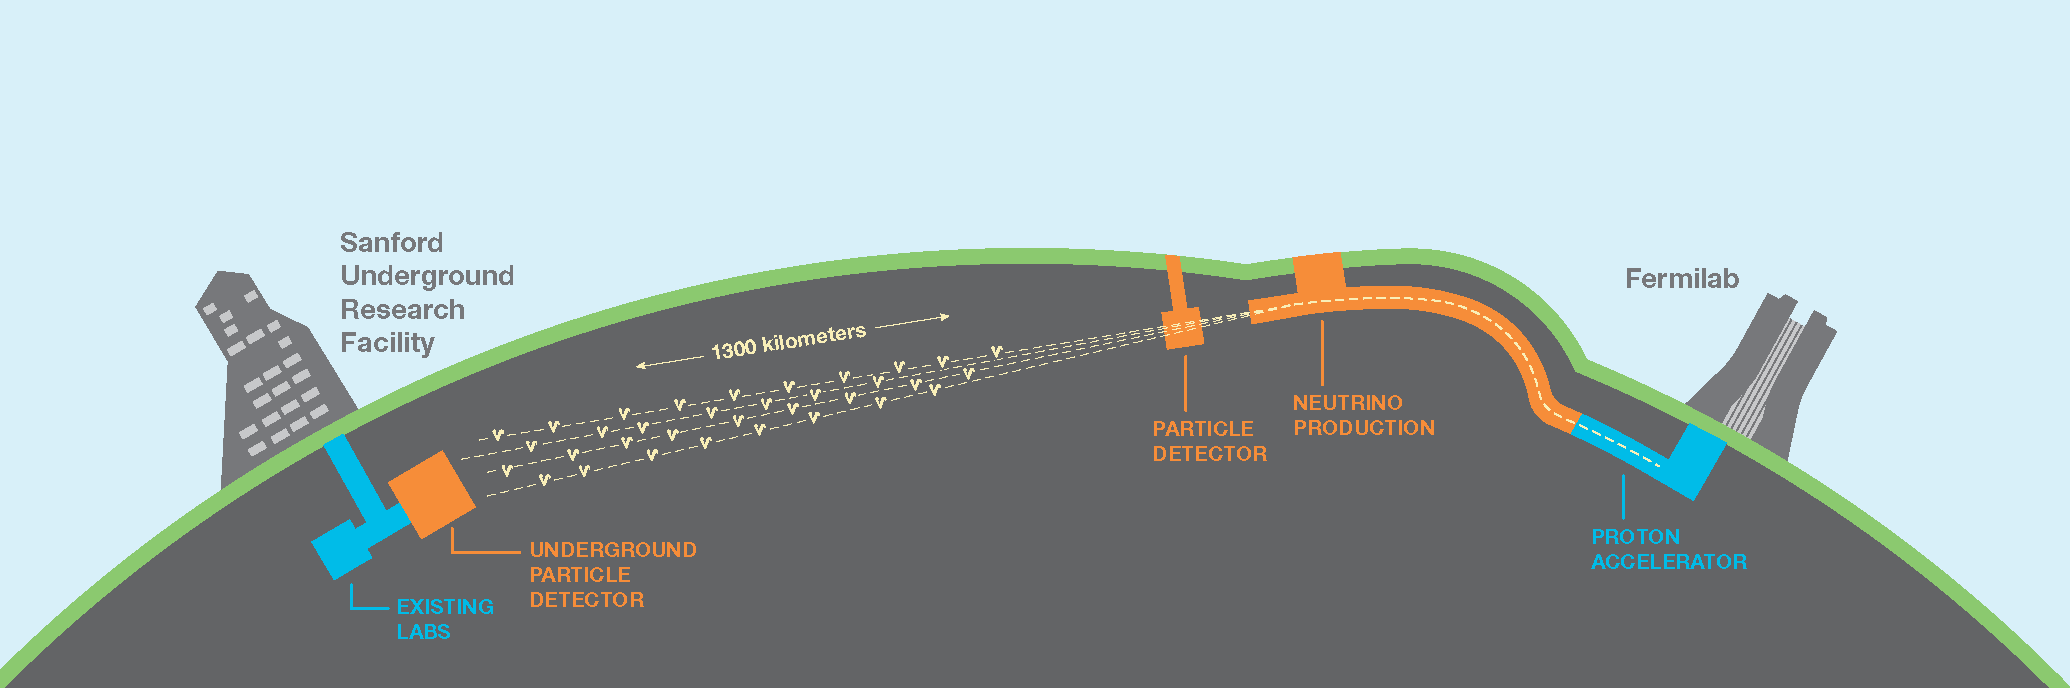
\includegraphics[width=\textwidth]{figures/dune_baseline.png}

	\caption
	[The Deep Underground Neutrino Experiment.]
	{The Deep Underground Neutrino Experiment. Figure from \cite{Abi:2020wmh}.}

	\label{fig:dune_baseline}

\end{figure}

The DUNE experiment will be a next generation neutrino physics and nucleon decay
experiment consisting of three principal components; an intense broad band 
neutrino beam, a precise Near Detector complex, and a Far Detector. The neutrino
beam and Near Detector complex will be based at the Fermilab National 
Accelerator Laboratory (FNAL) near Chicago, and the Far Detector will be based 
at Sanford Underground Research Facility (SURF) in South Dakota, approximately 
1300 km away from the neutrino source. The experimental setup is shown in Figure
\ref{fig:dune_baseline}. 

The DUNE experiment identifies three primary scientific goals\cite{Abi:2020evt}:
\begin{itemize}
	\item Perform a comprehensive programme of neutrino oscillation measurements
		including measurements of \dcp{}, neutrino mass ordering, and $\theta_{23}$.
	\item Search for proton decay in several decay modes.
	\item Measure neutrinos from a core--collapse supernova, if one occurs within 
		our galaxy during the lifetime of the experiment.
\end{itemize}
In addition, the experiment hopes to fulfill a significant programme of
secondary science goals:
\begin{itemize}
	\item Other accelerator based neutrino physics, such as non--standard
		interactions, sterile neutrinos, and CPT violation.
	\item Measurements of neutrino properties using atmospheric neutrinos.
	\item Dark matter searches in both the Near and Far Detectors.
	\item A programme of neutrino interaction physics studies in the DUNE Near
		Detector.
\end{itemize}

To achieve these goals, DUNE has opted to base the Near and Far Detector designs
on the liquid argon time projection chamber (LArTPC) technology. The DUNE
Far Detector will eventually consist of four LArTPC detectors each with 10 kt 
of active liquid argon mass. This technology will have never before been used 
on this scale and, therefore, there has been a significant ongoing programme 
of LArTPC research and development, to validate and characterise the performance
of the technology for DUNE. 

\subsection{Liquid Argon Time Projection Chambers}
A LArTPC consists of a large volume of highly--purified liquid argon, which is
subjected to an electric field. Charged particles traversing the liquid argon 
produce two primary energy depositions, a trail of ionisation electrons along 
their path, and prompt ultra--violet scintillation photons. After creation, 
the ionisation electrons drift in the electric field toward the charge readout 
plane, where they induce electrical signals. Liquid argon is transparent to 
its own scintillation light, therefore, the scintillation photons can travel 
through the argon to be collected in a photon detection system. The LArTPC 
detection principal is illustrated in Figure \ref{fig:lartpc}. 

\begin{figure}

	\centering

	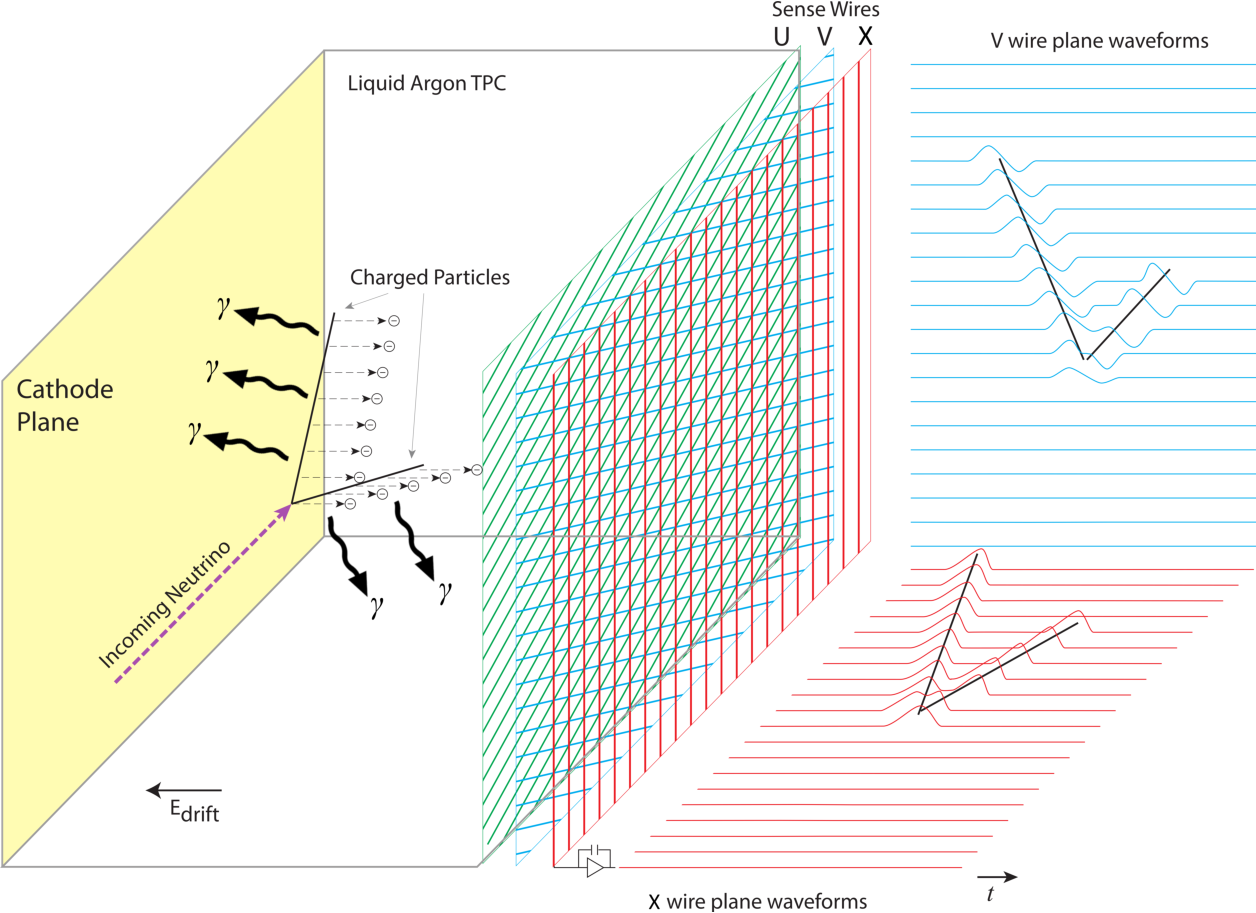
\includegraphics[width=\textwidth]{figures/LArTPC_Concept.pdf}

	\caption
	[A schematic of the LArTPC detection principal.]
	{A schematic of the LArTPC detection principal. Charged particles, in this
	case resulting from a neutrino interaction, produce two signals in the liquid
	argon, ionisation electrons and scintillation light. The ionisation electrons
	are drifted in the applied electric field and collected on a set of sense
	wires which record the signal. The scintillation photons are collected by 
	photon detectors, which are not depicted. Figure from \cite{Abi:2020loh}.}

	\label{fig:lartpc}

\end{figure}

\subsubsection*{The Role of Light in LArTPCs}

The ionisation signals in a LArTPC are slow, it takes electrons milliseconds to
travel from the cathode plane to the anode plane. In contrast, scintillation 
photons only take nanoseconds to reach the closest anode plane. This 
scintillation light plays an important role in the accurate 3D reconstruction 
of interactions in the LArTPC, as it can be used to determine the time of an 
interaction to within a few nanoseconds.

In a LArTPC, interactions play out much more quickly than the detector is able 
to record them, and each event actually integrates over a large number of 
interactions within the readout window. The true time, often referred to as 
the $t_0$, of the interactions in the event cannot be accurately reconstructed 
from the ionisation signals alone; by utilising the much faster scintillation 
signals, the time of interactions can be calculated with much higher 
precision.  This data can be combined with the arrival time of drifting 
electrons to reconstruct the true drift distance. Without an accurate $t_0$, 
the reconstructed drift distance will be incorrect, and as a result, so too
would the predicted charge attenuation.

Whilst the details of the charge readout and photon detection systems are unique
in each detector, LArTPC detectors can be split into two main categories: 
single--phase and dual--phase. In a single--phase detector, the drifting 
ionisation electrons remain in the liquid argon and the signals are usually 
read out on three anode wire planes, although pixel readout systems have also 
been developed\cite{argoncube}. A dual--phase LArTPC contains an additional 
region of gaseous argon, in which a high electric field, known as the 
extraction field, is applied to extract the ionisation from the liquid into 
the gas before it is amplified and collected on a pair of anode wire 
planes\cite{Abi:2020wmh}.

\bigskip\noindent
\protodune{} is one of two large scale prototypes for the DUNE Far Detector
modules, which focusses on the single--phase LArTPC technology. The DUNE Far
Detector is designed such that each module is built up of a number of 
identical components. \protodune{} was designed to prototype the design of 
many of these components at a 1:1 scale, including the anode planes, cathode 
plane, and photon detectors. The \protodune{} experiment has four primary 
goals, as outlined in the Technical Design Report\cite{Abi:2017aow}:
\begin{itemize}
	\item Prototype the production and installation procedures for the
		single--phase Far Detector design.
	\item Validate the design from the perspective of basic detector performance; this can be achieved with cosmic-ray data. 
	\item Accumulate large samples of test-beam data to understand/calibrate the
		response of the detector to different particle species.
	\item Demonstrate the long-term operational stability of the detector as part
		of the risk mitigation program ahead of the construction of the first 10 kt
		Far Detector module.
\end{itemize}
As such, \protodune{} represents a significant milestone in the development of
the Far Detector for the DUNE experiment. Its successful operation, both in a 
test beam and with cosmic--rays, provides valuable data with which to understand
reconstruction and analysis of the data that will be collected by the DUNE Far 
Detector.

\section{The \protodune{} Detector} \label{sec:pdsp_detector}

The \protodune{} detector is located at the Neutrino Platform at CERN along the
H4 beamline. It is a single--phase LArTPC detector with a total liquid argon 
mass of 0.77 kt, making it the largest monolithic single--phase liquid argon TPC
at the time of writing. The TPC comprises the following major components, which 
are illustrated in Figure \ref{fig:pdsp_tpc}:
\begin{itemize}
	\item A cathode plane constructed of modular cathode plane assemblies (CPA).
	\item Two anode planes constructed of modular anode plane assemblies (APA).
	\item A photon detection system (PDS), which is integrated into the APAs.
	\item A field cage, beam plug, and high voltage systems.
	\item Readout electronics and data acquisition system (DAQ).
\end{itemize}
The detector components are designed to be an almost exact replica of the final 
single--phase Far Detector modules, but the detector has an overall scaling 
factor of approximately $1:20$ in terms of total liquid argon 
mass\cite{Abi:2017aow}.

\begin{figure}

	\centering

	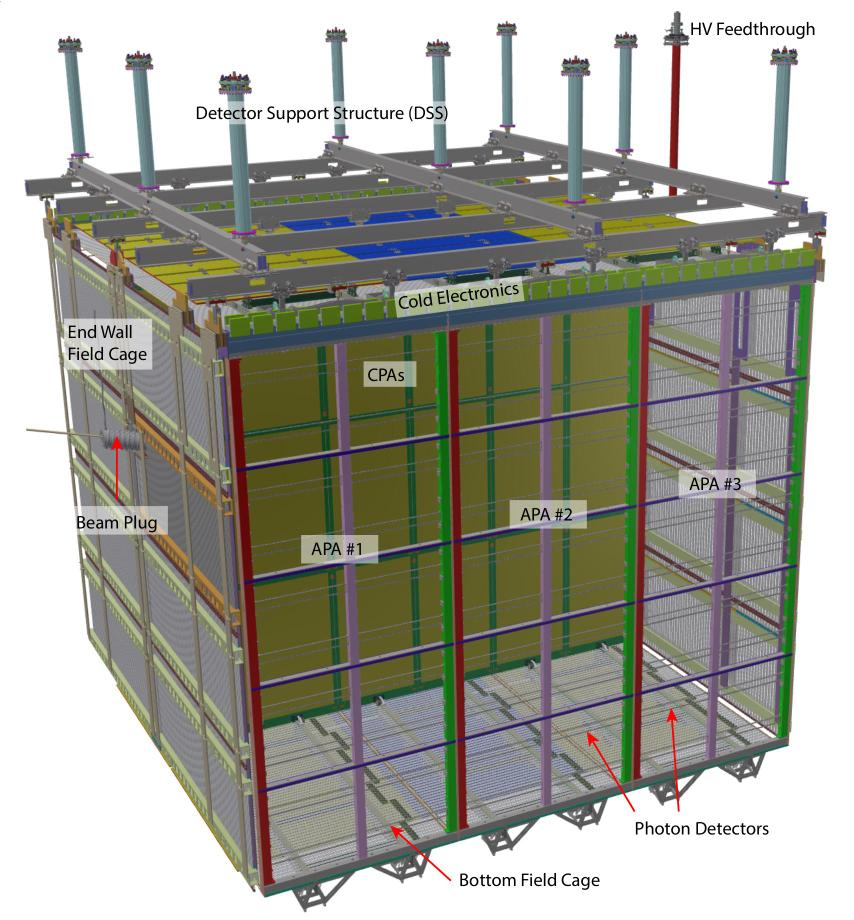
\includegraphics[width=0.9\textwidth]{figures/pdsp_tpc.jpg}

	\caption
	[A 3D rendering of the main components of the \protodune{} TPC.]
	{A 3D rendering of the main components of the \protodune{} TPC, with the main
	components labelled. Figure from \cite{Abi:2017aow}.}

	\label{fig:pdsp_tpc}

\end{figure}

\subsection{The Liquid Argon TPC}

The \protodune{} TPC has an active volume of 6 m (height) $\times$ 7.2 m (width,
drift direction) $\times$ 7 m (length, approximate beam direction). The cathode 
plane at the center of the active width is flanked by two anode planes, which 
define two 3.6 m drift volumes. The field cage around these two drift volumes
helps to ensure a uniform electric field within the drift region.

Each anode plane is modularly constructed from three APAs, which have dimensions
6 m (height) $\times$ 2.3 m (width). The APA frame holds three sets of parallel
wires on the inward and outward facing sides, these are oriented at different 
angles to enable 3D reconstruction. The outer two sets of wires are induction
wires, these are biased such that they are electrically transparent to the 
drifting ionisation. Ionisation passing the induction wires causes an induced 
bi--polar signal. The third set of wires are known as collection wires, which
are not biased. When drifting ionisation approaches the collection wires 
it is absorbed producing a uni--polar signal. In \protodune{}, each set of 
induction wires contains 800 wires at a spacing of 4.67 mm, and each set of 
collection wires contains 480 wires at a spacing of 4.79 mm. 

The wire planes from each APA are read out by electronics boards, known as
front--end mother boards (FEMB), which are mounted on the APA frame. The FEMBs 
are submerged in the liquid argon and, therefore, they are also referred to as 
cold electronics (CE). A total of 2560 electronics channels are used to read 
out the data from each APA, with each readout window corresponding to 3 ms, 
which is 6000 time samples. The CE amplify, shape, and digitise the signals 
from the wires before transmitting them outside the TPC to the warm interface 
boards (WIB). The WIBs collate the data from the CE boards and pass the data 
onto the data acquisition system (DAQ).

The cathode plane in \protodune{} consists of an array of 18 CPA modules, 2 m 
(height) $\times$ 1.2 m (width). The cathode plane is held at -180 kV to 
provide a 500 $\mbox{V/cm}$ drift field in each of the drift volumes. The 
field cage surrounding the drift regions ensures that the electric field is 
uniform across the detector volume, by providing the necessary electrical
boundary conditions.

One area in which the design of \protodune{} differs from the Far Detector is
the inclusion of the beam plug. This is necessary to minimize interactions
between the charged particle test beam and the cryostat before the beam enters 
the active region of the detector. A cylindrical beam plug, which contains 
nitrogen gas, penetrates from the cryostat wall into the field cage at 
location of the incoming test beam. 

\subsection{The Photon Detection System}

The Photon Detection System (PDS) in \protodune{} is integrated into the APAs. 
Ten photon detector modules are embedded in each APA frame between the layers 
of wires on either side of the APA, as shown in Figure \ref{fig:pdsp_tpc}. 
Three types of photon detector module were tested in \protodune{}, two very 
similar module designs based on coupling silicon photomultipliers to 
wavelength shifting bars, and a third novel design known as the ARAPUCA light 
trap. The operating principles of the two designs are illustrated in Figure 
\ref{fig:pdsp_pd}.

\begin{figure}

	\centering

	\begin{subfigure}[b]{0.29\textwidth}
		\centering
		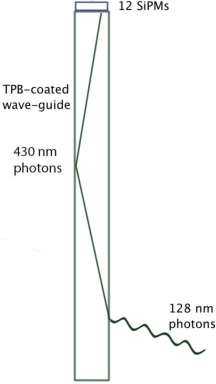
\includegraphics[width=0.95\textwidth]{figures/pdsp_pd.pdf}
		\caption{Waveguide.}
		\label{fig:pd_bars}
	\end{subfigure}
	\begin{subfigure}[b]{0.69\textwidth}
		\centering
		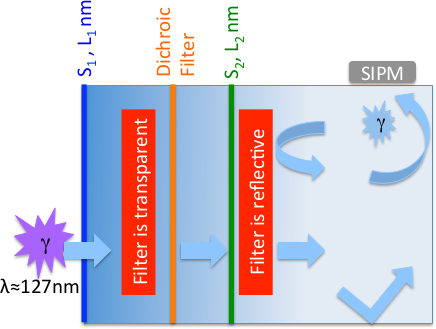
\includegraphics[width=0.95\textwidth]{figures/pdsp_arapuca.png}
		\caption{ARAPUCA.}
		\label{fig:arapuca}
	\end{subfigure}

	\caption
	[The operating principal of the photon detector modules in \protodune{}.]
	{The operating principal of the two main types of photon detector module in 
	\protodune{}. Figure \subref{fig:pd_bars} from \cite{Abi:2017aow}. Figure 
	\subref{fig:arapuca} from \cite{Machado:2016jqe}.}

	\label{fig:pdsp_pd}

\end{figure}

The majority of the photon detector modules in \protodune{} consist of 
wavelength shifting bars coupled to silicon photomultipliers (SiPM). 
Tetraphenyl-butadiene (TPB) is used to shift the wavelength of the light 
from ultra--violet to blue before the light is transmitted down the waveguide to
the SiPMs. The main difference between the two nominal designs is in the 
wavelength of transmission within the waveguide. In one case the wavelength is 
transmitted at the blue wavelength produced by the TPB, in the other case the 
blue light from the TPB is first absorbed in the waveguide which then produces 
green light which is transmitted down the waveguide.

A small number of the photon detector modules in \protodune{} feature a novel 
design known as an ARAPUCA light trap. In this design the photons are trapped 
in a small box through a sequence of wavelength shifting and optical 
filtering, thereby significantly increasing the photon detection 
efficiency\cite{Segreto:2018jdx}. An ARAPUCA light trap consists of a box 
which is high reflective on the inside. On one side of the box is 
the filtering window, and on the other a SiPM. Incoming ultra--violet photons 
are shifted to the blue spectrum before passing through a dichroic filter 
which has a tunable wavelength cut--off, after which it transitions from being 
transparent to reflective. After passing through the filter the photons are 
shifted again, this time from blue to green, such that the filter becomes
reflective to them. Consequently green photons can be trapped within the 
ARAPUCA until they come into contact with the SiPM, this provides increased 
photon detection efficiency. Each ARAPUCA photon detector module in 
\protodune{} features an array of these traps arranged in a line across the 
width of an APA. The ARAPUCA modules contain 12 ARAPUCA light traps, these are 
constructed from 16 so called cells, which are 5 cm $\times$ 5 cm $\times$ 1 
cm boxes.  Half of the light traps are made of one cell and the others are 
made of two cells joined together. Regardless of the number of cells, each 
ARAPUCA trap is read out by a single SiPM, making for 12 SiPMs per ARAPUCA 
module.

Unlike with the TPC electronics, there are no front--end electronics in the LAr
volume for the PDS, the unamplified analogue signals are transmitted out of the
cryostat before processing and digitisation. The light guide based photon 
detector modules have 12 SiPMs, which are read out in threes meaning that each 
module corresponds to 4 readout channels. The ARAPUCA modules are read out by
one channel per SiPM, resulting in 12 channels per ARAPUCA module. The readout 
channels from each APA are processed by four so called SiPM signal processors 
(SSP), which are mounted on the top of the cryostat. After processing in the 
SSPs, the PDS data is passed onto the DAQ along with the TPC data.

\section{The H4 beamline} \label{sec:h4}

The \protodune{} experiment is located at the end of the H4 beamline at CERN,
the location of the beamline with respect to the detector is illustrated in
Figure \ref{fig:pdsp_CRT}. The beam has a mixture of particle types including
hadrons, muons, and electrons, with momenta in the range 0.3--7 GeV. The momenta
and composition of the beam can be varied, several runs were taken across a 
range of particle compositions and beam momenta.

The H4 beamline is a tertiary beamline, which is produced when a secondary beam
from the T2 primary target interacts with a target. Particles from the 
secondary target are selected based on momentum and charge before travelling 
down the H4 beamline to \protodune{}. A schematic of the beamline 
instrumentation (BI) and magnets in the H4 beamline is given in Figure 
\ref{fig:h4_schem}. 

\begin{figure}

	\centering

	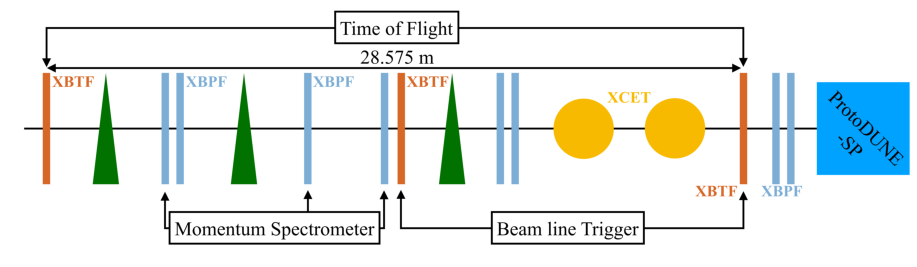
\includegraphics[width=\textwidth]{figures/h4_schem.pdf}

	\caption
	[A schematic of the H4 beamline magnets and instrumentation.]
	{A schematic of the H4 beamline magnets and instrumentation. There are eight
	profile monitors, three trigger counters, and two threshold Cerenkov counters,
	labelled XBPF, XBTF, and XCET respectively. The bending magnets are depicted
	as green triangles. The data from these components is combined for triggering,
	measuring the beam momentum, and measuring the time of flight of beam
	particles. The components used for each of these tasks are labelled above and
	below the beamline schematic. Figure from \cite{protoduneperf}.}

	\label{fig:h4_schem}

\end{figure}

By combining momentum measurements from the profile monitors with time of flight
(TOF) and Cerenkov measurements, the beam momentum and composition can be 
measured. The predicted and measured distribution of TOF vs momentum for data,
from a number of runs at different momenta, is shown in Figure \ref{fig:h4_tof}.
This information is used to trigger the detector during beam running, and is
sent to the central trigger board for distribution to the detector components.

\begin{figure}

	\centering

	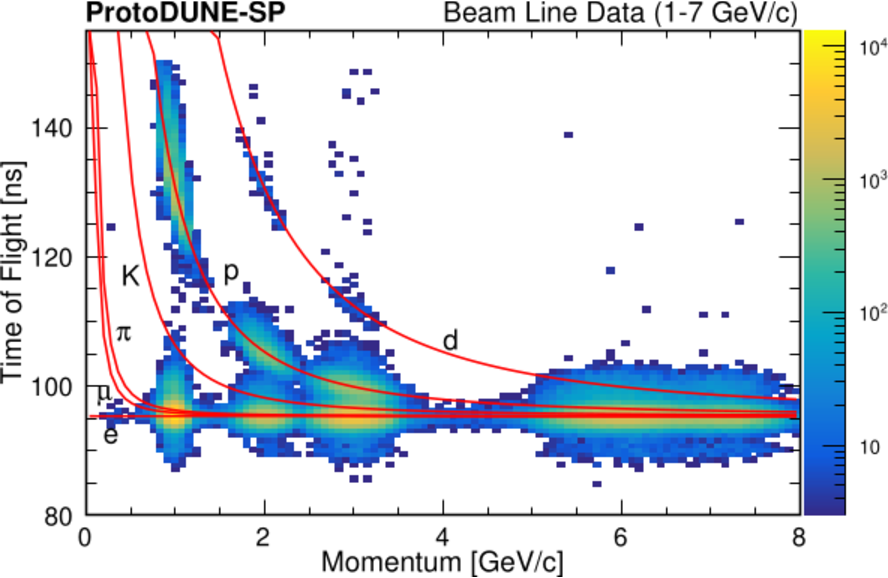
\includegraphics[width=\textwidth]{figures/h4_tof.pdf}

	\caption
	[Time of flight vs momentum distributions from the H4 beamline
	instrumentation.]
	{Time of flight vs momentum distributions from the H4 beamline
	instrumentation, for \protodune{} runs at average momenta from 1--7 GeV. The
	simulated distributions for different beam particle species are labelled on
	the figure. Figure from \cite{protoduneperf}.}

	\label{fig:h4_tof}

\end{figure}

During the beam running period, a number of runs were taken with differing beam
compositions and momenta. A summary of the collected beam data, as well as
predictions of the particle composition from beamline simulations, is given in 
Table \ref{tab:beam_runs}.
\begin{table}
	\centering
	\begin{tabular}{c|c|c|c|c|c|c}
		\thead{Momentum \\ (GeV/c)} & \thead{Recorded \\ Triggers \\ ($10^3$)} &
		\thead{Expected \\Triggers \\ ($10^3$)} & \thead{Expected \\ Pions \\ ($10^3$)} &
		\thead{Expected \\Protons \\ ($10^3$)} & \thead{Expected \\Electrons \\ ($10^3$)} &
		\thead{Expected \\ Kaons \\ ($10^3$)} \\ \hline
		0.3 & 269  & 242  & 0      & 0     & 242  & 0 \\
		0.5 & 340  & 299  & 1.5    & 1.5   & 296  & 0 \\
		1   & 1089 & 1064 & 382    & 420   & 262  & 0 \\
		2   & 728  & 639  & 333    & 128   & 173  & 5 \\
		3   & 568  & 519  & 284    & 107   & 113  & 15 \\
		6   & 702  & 689  & 394    & 70    & 197  & 28 \\
		7   & 477  & 472  & 299    & 51    & 98   & 24 \\ \hline
		All & 4173 & 3924 & 1693.5 & 777.5 & 1381 & 72 \\
	\end{tabular}

	\caption
	[Summary of expected and recorded beam triggers in \protodune{}.]
	{ Summary of expected and recorded beam triggers in \protodune{}. The number
	of expected triggers represents the number of triggers expected in the initial
	\protodune{} run plan, which are exceeded at every energy. The breakdown of
	expected triggers by particle species is based on simulations of the
	H4 beam--line. Data from \cite{Spanu_2019}.}

	\label{tab:beam_runs}

\end{table}

\section{The Cosmic--Ray Tagger} \label{sec:pdsp_cosmic}

As a surface level detector with no overburden \protodune{} measures a
significant rate, on the order of 20 kHz, of cosmic--ray muons. This corresponds
to an average of 60 muons per 3 ms readout window. These muons provide a 
useful source of calibration data in the form of long tracks and stopping 
muons.  The cosmic--ray tagger (CRT) in \protodune{} was installed on the 
upstream and downstream faces of the TPC, to trigger the detector for 
cosmic--ray muons which travel parallel to the anode plane. In addition the 
CRT, can provide accurate timing information for any tracks which are
successfully matched between the TPC and CRT.

The CRT consists of four parts, two upstream assemblies and two downstream
assemblies, the locations of the CRT assemblies is illustrated in Figure
\ref{fig:pdsp_CRT}. Each CRT assembly is constructed from overlapping 
scintillation counters, which cover an area 6.8 m high and 3.65 m wide. 
Scintillation strips of length 365 cm and width 5 cm are placed in 
perpendicular arrays to give 2D reconstruction within each CRT 
assembly. By combining data from upstream and downstream CRT assemblies, with a 
time coincidence requirement, the 3D trajectories of tracks can be 
reconstructed.

\begin{figure}

	\centering

	\begin{subfigure}[b]{\textwidth}
		\centering
		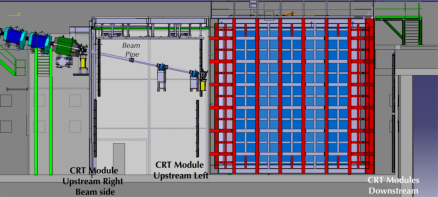
\includegraphics[width=0.9\textwidth]{figures/crt_side.pdf}
		\label{fig:crt_side}
		\caption{Side view.}
	\end{subfigure}

	\vspace{3mm}

	\begin{subfigure}[b]{\textwidth}
		\centering
		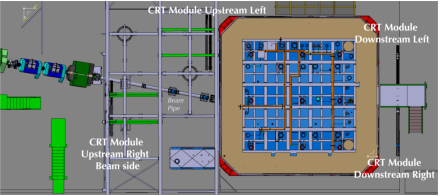
\includegraphics[width=0.9\textwidth]{figures/crt_top.pdf}
		\label{fig:crt_top}
		\caption{Top view.}
	\end{subfigure}

	\caption
	[Location of the H4 beamline and cosmic--ray taggers in relation to the
	\protodune{} detector.]
	{A rendering of the location of the H4 beamline and cosmic--ray taggers in 
	relation to the \protodune{} detector. The CRT modules are labelled on the
	figures, in both the side view and the top view. Figures from 
	\cite{protoduneperf}.}

	\label{fig:pdsp_CRT}

\end{figure}

\section{The Data Acquisition System}

Data from the TPC, PDS, and CRT in \protodune{} are collated by the data 
acquisition system (DAQ). The DAQ distributes triggers, compresses and packages 
the data into events, and stores the data ready for future analysis. 
An overview of the \protodune{} DAQ system is seen in Figure 
\ref{fig:pdsp_daq}; there are four primary data flows in the system: TPC, PDS, 
CRT, and BI. Timing and triggering signals are distributed to the detector 
components by the timing board, which maintains a 50 MHz clock and receives 
$\sim 40 \mbox{Hz}$ of triggers from the central trigger board (CTB) based on 
data from the BI and CRT\cite{Abi:2017aow}.

\begin{figure}

	\centering

	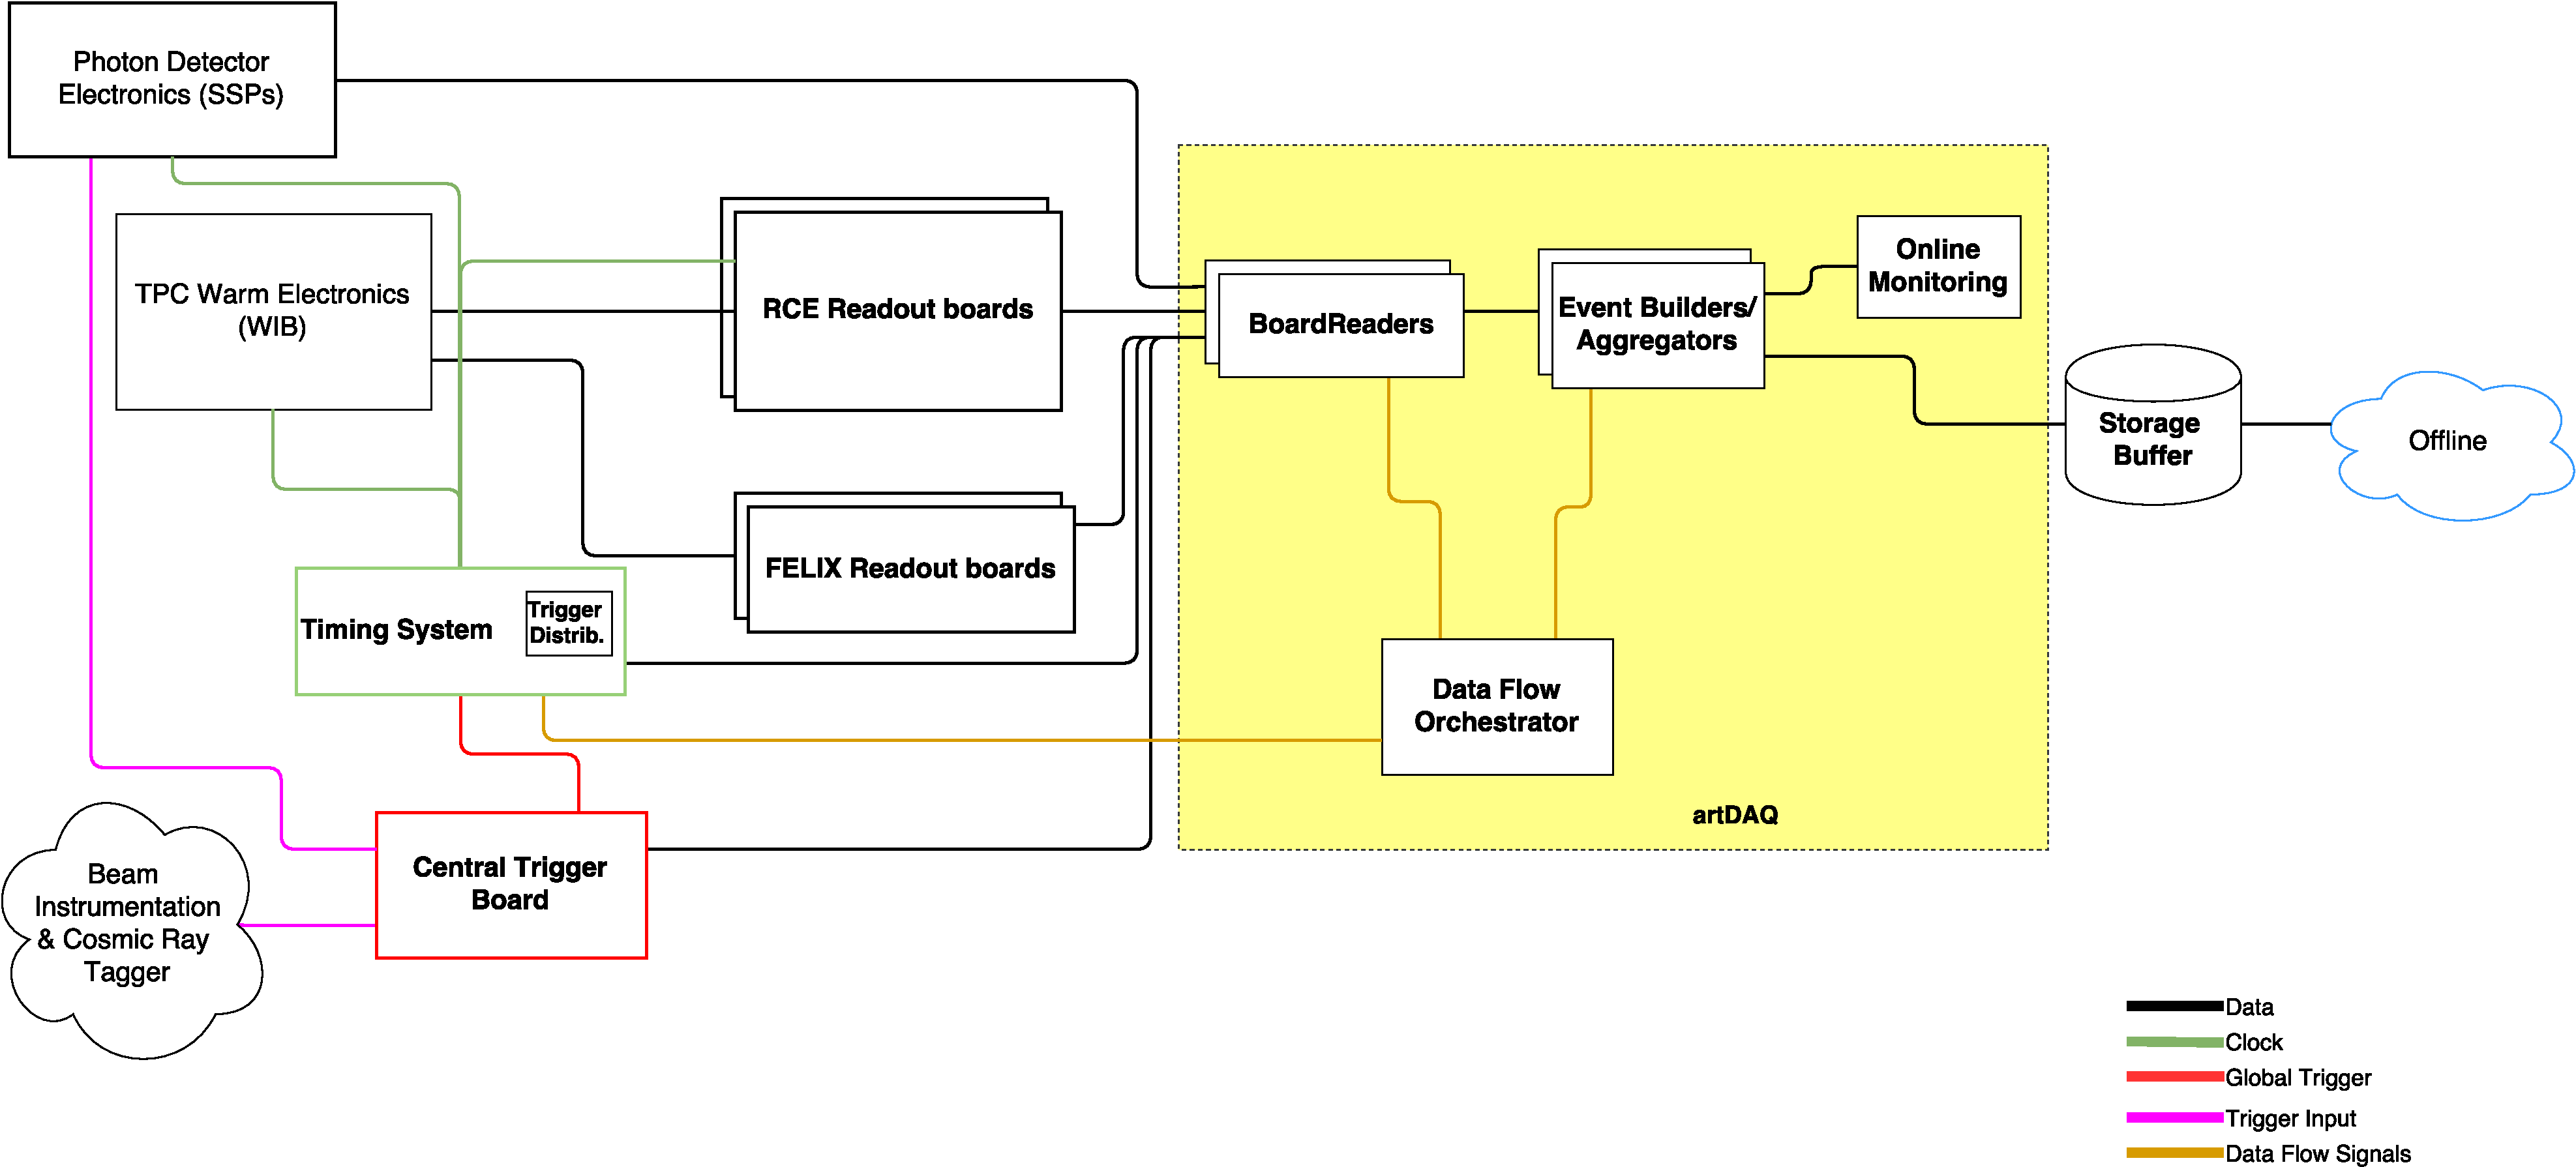
\includegraphics[width=\textwidth]{figures/pdsp_daq.pdf}

	\caption
	[Outline of the data acquisition system in \protodune{}.]
	{Outline of the data acquisition system in \protodune{}, showing the data flow
	from the detector components through to offline storage ready for later
	analysis. The main elements of the system are shown, including the important 
	software components, which are part of the ArtDAQ framework highlighted by 
	the yellow box. Figure from \cite{Abi:2017aow}.}

	\label{fig:pdsp_daq}

\end{figure}

The \protodune{} TPC contains a total of 15,360 wires spread across the six
APAs. The wires are digitized at a rate of 2 MHz, resulting in an overall data
flow of around 480 $\mbox{Gb/s}$ from the TPC electronics. An event in
\protodune{} corresponds to a continuous readout of the detector for 3 ms,
resulting in 6000 samples from each wire; data is buffered such that the readout
window can be opened 250 $\mu$s before the trigger time. Data from the TPC is
received by two systems, one system, which is based on Reconfigurable Computing Elements
(RCE)\cite{7431254}, handles the data from five APAs, while the other system
handles the data from the sixth APA, and is based on front--end link exchange 
(FELIX) cards, which have been developed by the ATLAS 
collaboration\cite{Anderson_2016}.

The software layer of the \protodune{} DAQ is based on Fermilab's 
ArtDAQ\cite{6495515}. This component is primarily responsible for acquiring 
the data, packaging it, and storing it locally. Triggered events are queued 
and distributed to the board readers and event builders by the data flow 
orchestrator. There are multiple board readers, which are each responsible for 
processing the data from specific hardware components. Details vary between 
specific board readers, but generally these processes are responsible for 
formatting the data from each component ready for aggregation. Data from the 
various detector components is aggregated by the event builders, which are 
responsible for assembling the completed events. After compression, events have 
an average size of 60 MB. ArtDAQ is also responsible for the real--time 
monitoring of data quality via the online monitoring system, this system will 
be discussed in Section \ref{sec:pdsp_om}.

\section{Simulation} \label{sec:simulation}

Simulation and reconstruction of \protodune{} data takes place in the LArSoft
framework\cite{Snider2017}. LArSoft is a software suite for simulating and
reconstructing data collected by LArTPC detectors, based on the Art event 
framework from Fermilab\cite{Green:2012gv}. LArSoft is under active use and
development by a number of participating LArTPC based experiments, with each
experiment making use of its core functionality, in addition to experiment 
specific code. 

Simulation in LArSoft is broken down into three sequential stages: generation,
propagation, and detector simulation. The initial state particles are produced
in the generation step, the propagation and interaction of these particles is 
simulated during the propagation step and finally the transport of energy 
depositions, and simulation of detector effects are handled by the detector 
simulation phase.

As a surface based detector in a test beam, \protodune{} is subject to three
main sources of particles: beam particles, cosmic--rays, and radiological 
decays. The beam particle flux in the vicinity of \protodune{} was provided by 
simulations of the H4 beamline\cite{Booth:2019brj} based on two simulation 
frameworks, G4beamline\cite{g4beamline} and FLUKA\cite{BOHLEN2014211}. The flux
of cosmic--ray particles in \protodune{} is simulated using 
CORSIKA\cite{Heck:1998vt}.  Finally, low energy radiological backgrounds in 
liquid argon are simulated, these include $^{39}\mbox{Ar,} ^ {85}\mbox{Kr, and }
^{222}\mbox{Rn}$.

After generation, the particles are allowed to propagate and interact in the 
detector geometry, including the cryostat, external systems, and experimental
hall. This is simulated using GEANT4\cite{Agostinelli:2002hh}, which tracks 
particles in small steps; the step size, $300 \mbox{ } \mu m$, is chosen to be 
much smaller then the spatial resolution of the detector to allow for 
small--scale processes like showering to be accurately simulated. 

Particles which propagate through the detector, during the propagation phase of
the simulation, leave energy deposits in the form of ionisation electrons and
scintillation photons. A minimum--ionising particle (MIP), which deposits 
around 2 MeV/cm in liquid argon, will produce tens of thousands of electrons 
and photons per cm.

The detector simulation is responsible for drifting the ionisation electrons 
towards the collection wires, propagating the simulated photons to the photon 
detectors, and simulating the response of the wires, SiPMs, and electronics to 
the signals. The shear number of ionisation electrons and scintillation 
photons produced in a \protodune{} event makes simulating the propagation of 
the full set of particles impractical and, therefore, LArSoft employs 
approximation techniques to predict the observed signals within a reasonable 
computation time. A number of detector effects are taken into account when 
simulating the electron drift: electron--ion recombination, transverse and 
longitudinal diffusion, electric field distortions, and electron capture on 
impurities. 

When the ionisation and scintillation signals arrive at the active detector 
components, simulated waveforms are produced based on the induced signals 
produced in the detector components. These signals are converted into 
electrical signals by electronics simulation, which is completed in LArSoft. 
The electronics simulation includes simulation of electronics gain, noise, 
and analogue to digital conversion. The simulated waveforms produced by the 
\protodune{} simulation are then compressed and stored ready for reconstruction.

\section{Reconstruction} \label{sec:reconstruction}

An event consists of a synchronised set of waveforms from all of the TPC 
channels, with each event corresponding to 3 ms or 6000 samples. The particle
interactions within each event are reconstructed into tracks and showers, 
which can be used for physics analyses, this section provides a brief summary 
of the steps involved in this reconstruction.

First, the TPC waveforms are passed through a set of filtering algorithms which
are designed to reduce the noise on the waveforms, as well as to mitigate 
effects from the electronics such as sticky--codes and undershooting. An 
additional step, known as a 2D deconvolution, is applied to extract the original
signal from the measured signal, based on a detector response function for 
both the wire in question and the neighboring wires. This method has been 
described in detail by the MicroBooNE collaboration\cite{Adams:2018dra}. An 
important side effect of the 2D deconvolution technique is that, after 
deconvolution, the bi--polar induction signals become unipolar, which 
simplifies hit reconstruction. An example of the noise filtering and 2D 
deconvolution techniques applied to a 7 GeV test beam event in \protodune{} 
data is given in Figure \ref{fig:2d_deconv}. 

\begin{figure}

	\centering

	\begin{subfigure}{0.49\textwidth}
		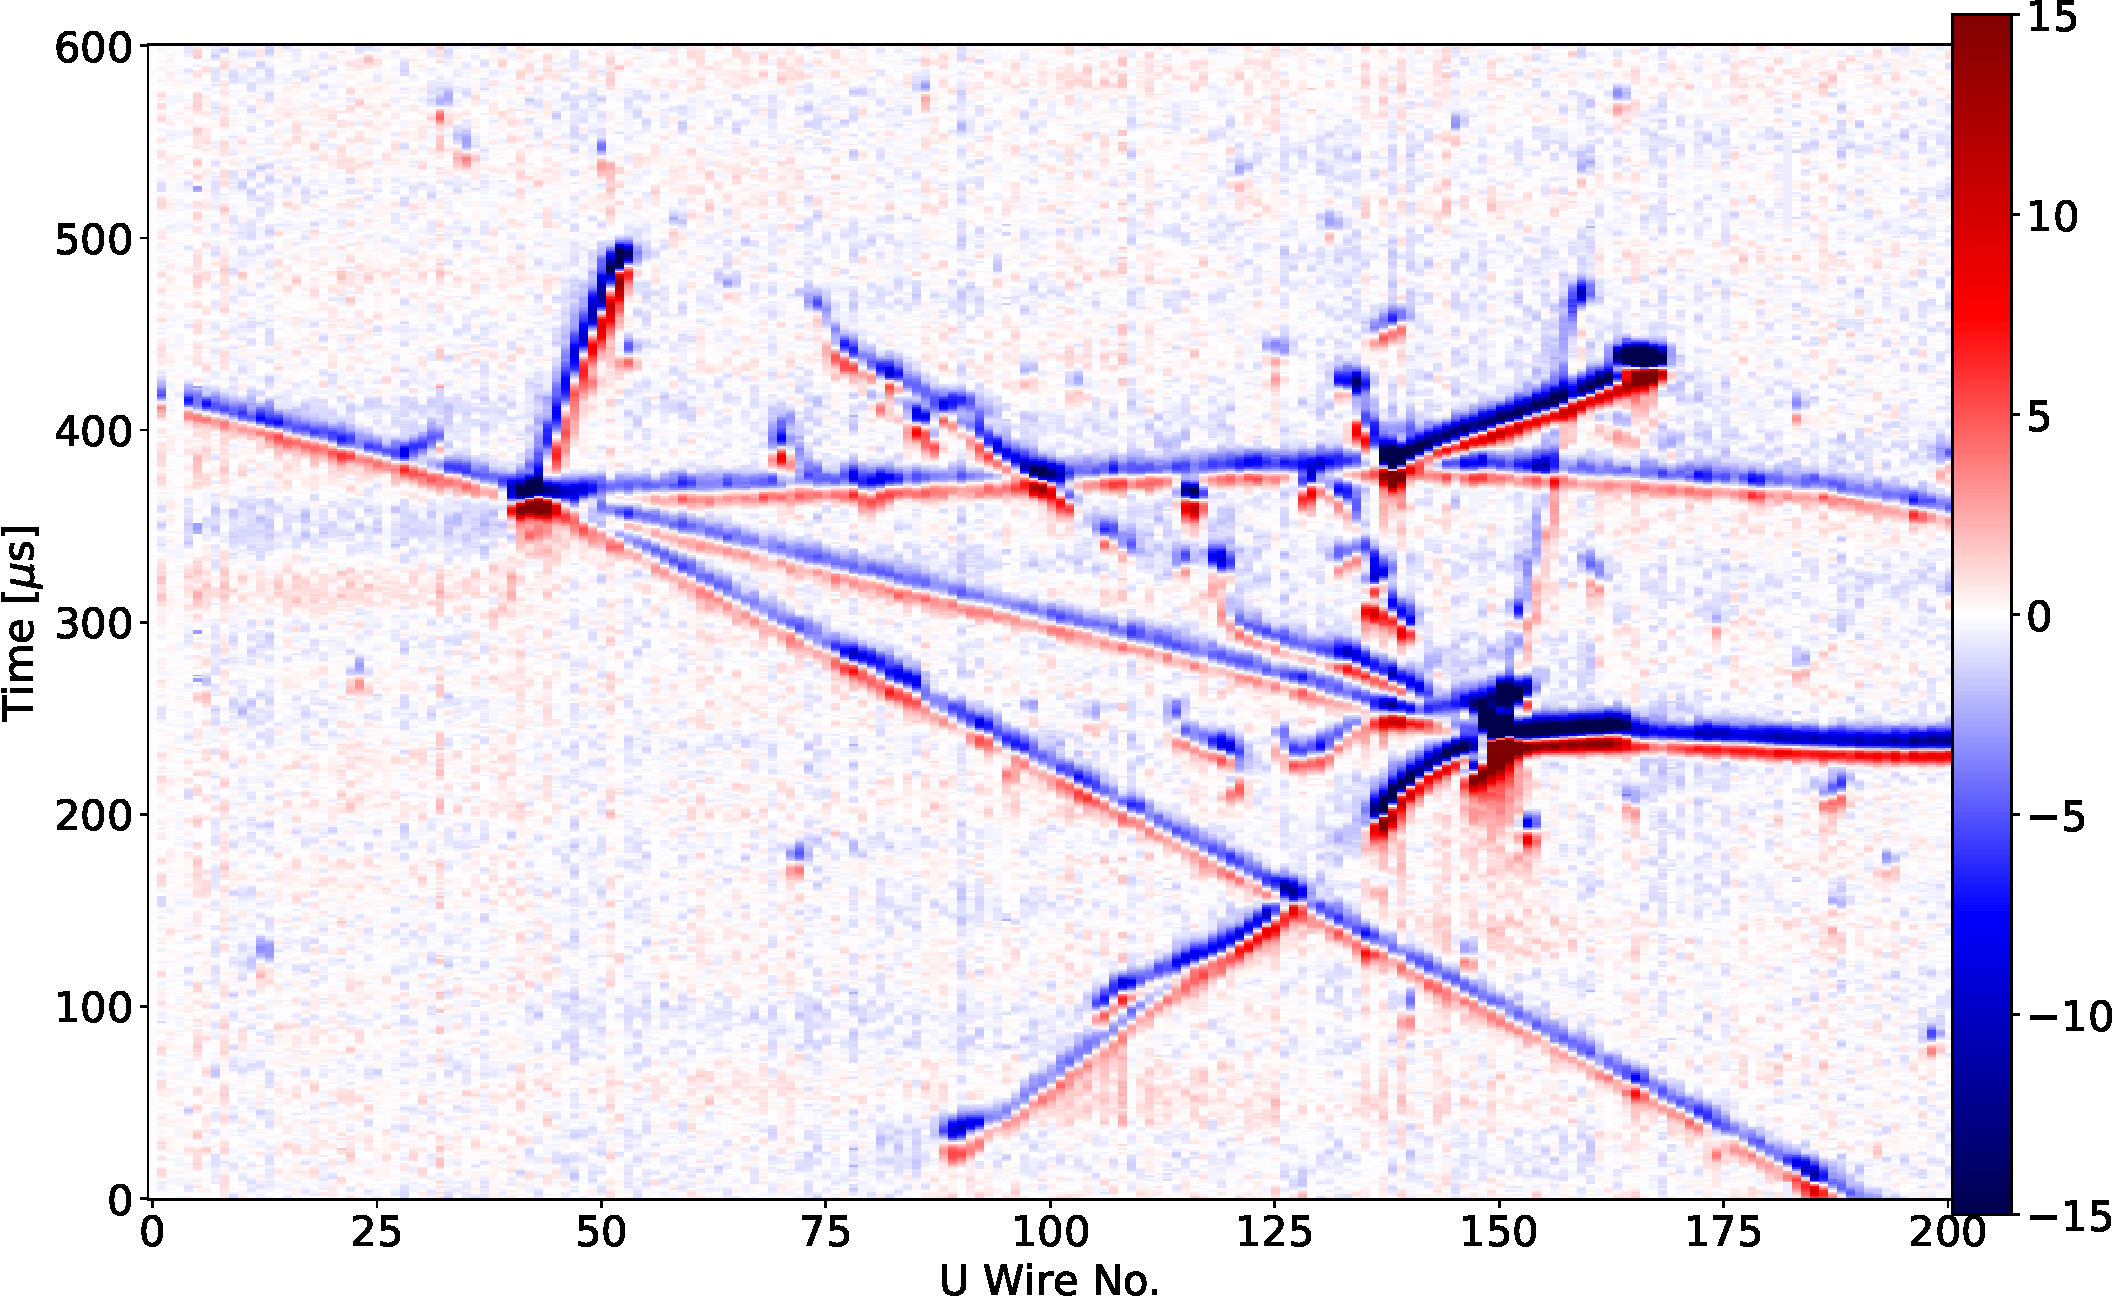
\includegraphics[width=\textwidth]{figures/protodune_evd_orig.pdf}
		\label{fig:pdsp_raw}
		\caption{Before noise filtering.}
	\end{subfigure}
	\hfill
	\begin{subfigure}{0.49\textwidth}
		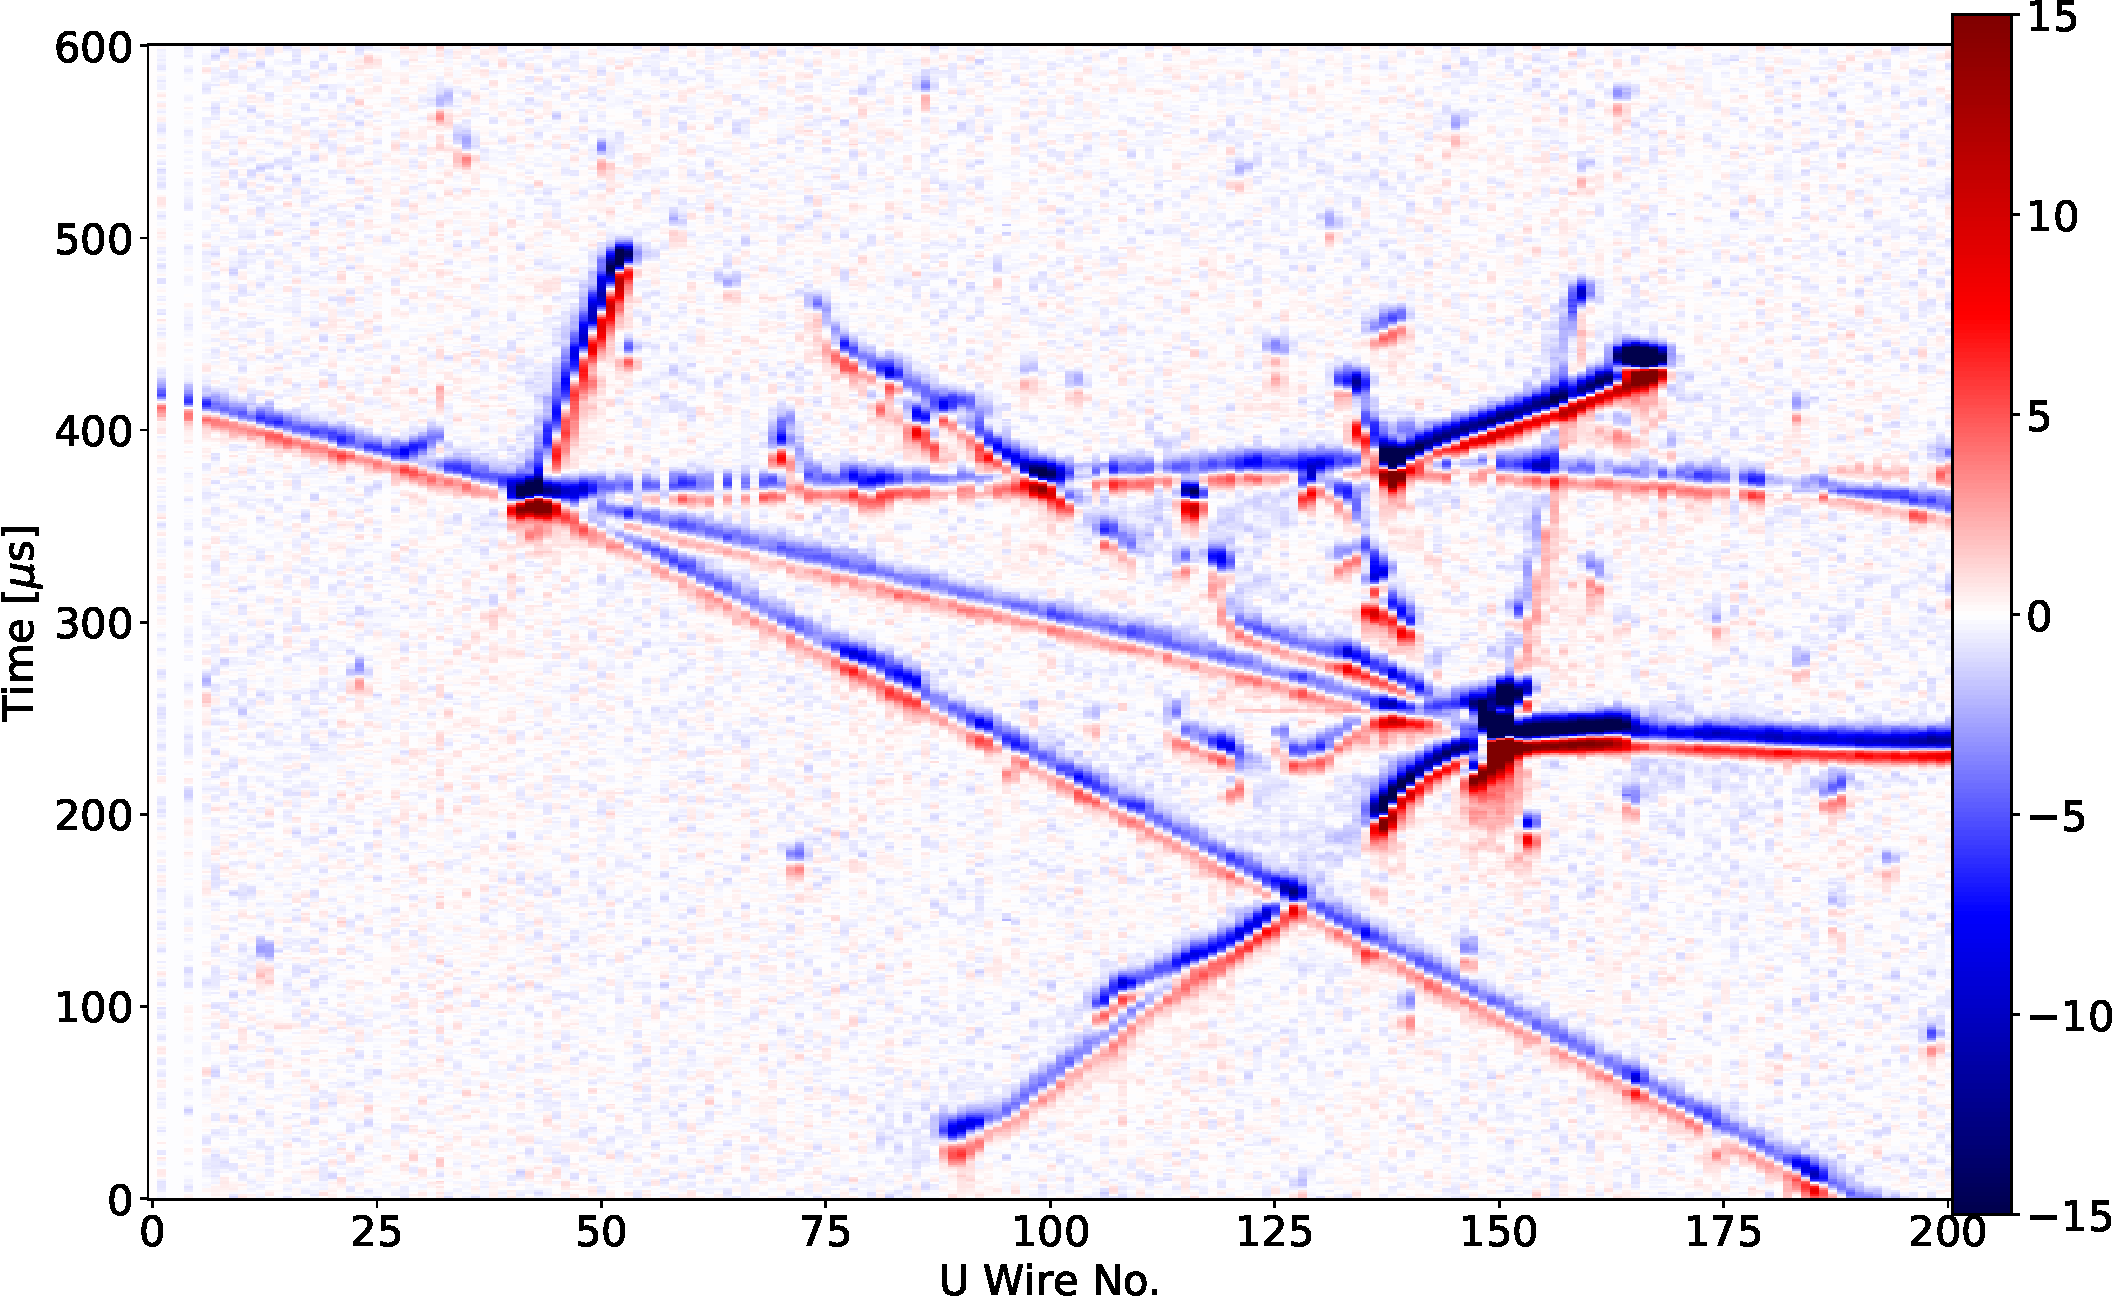
\includegraphics[width=\textwidth]{figures/protodune_evd_raw.pdf}
		\label{fig:pdsp_filt}
		\caption{After noise filtering.}
	\end{subfigure}
	\begin{subfigure}{0.49\textwidth}
		\vspace{5mm}
		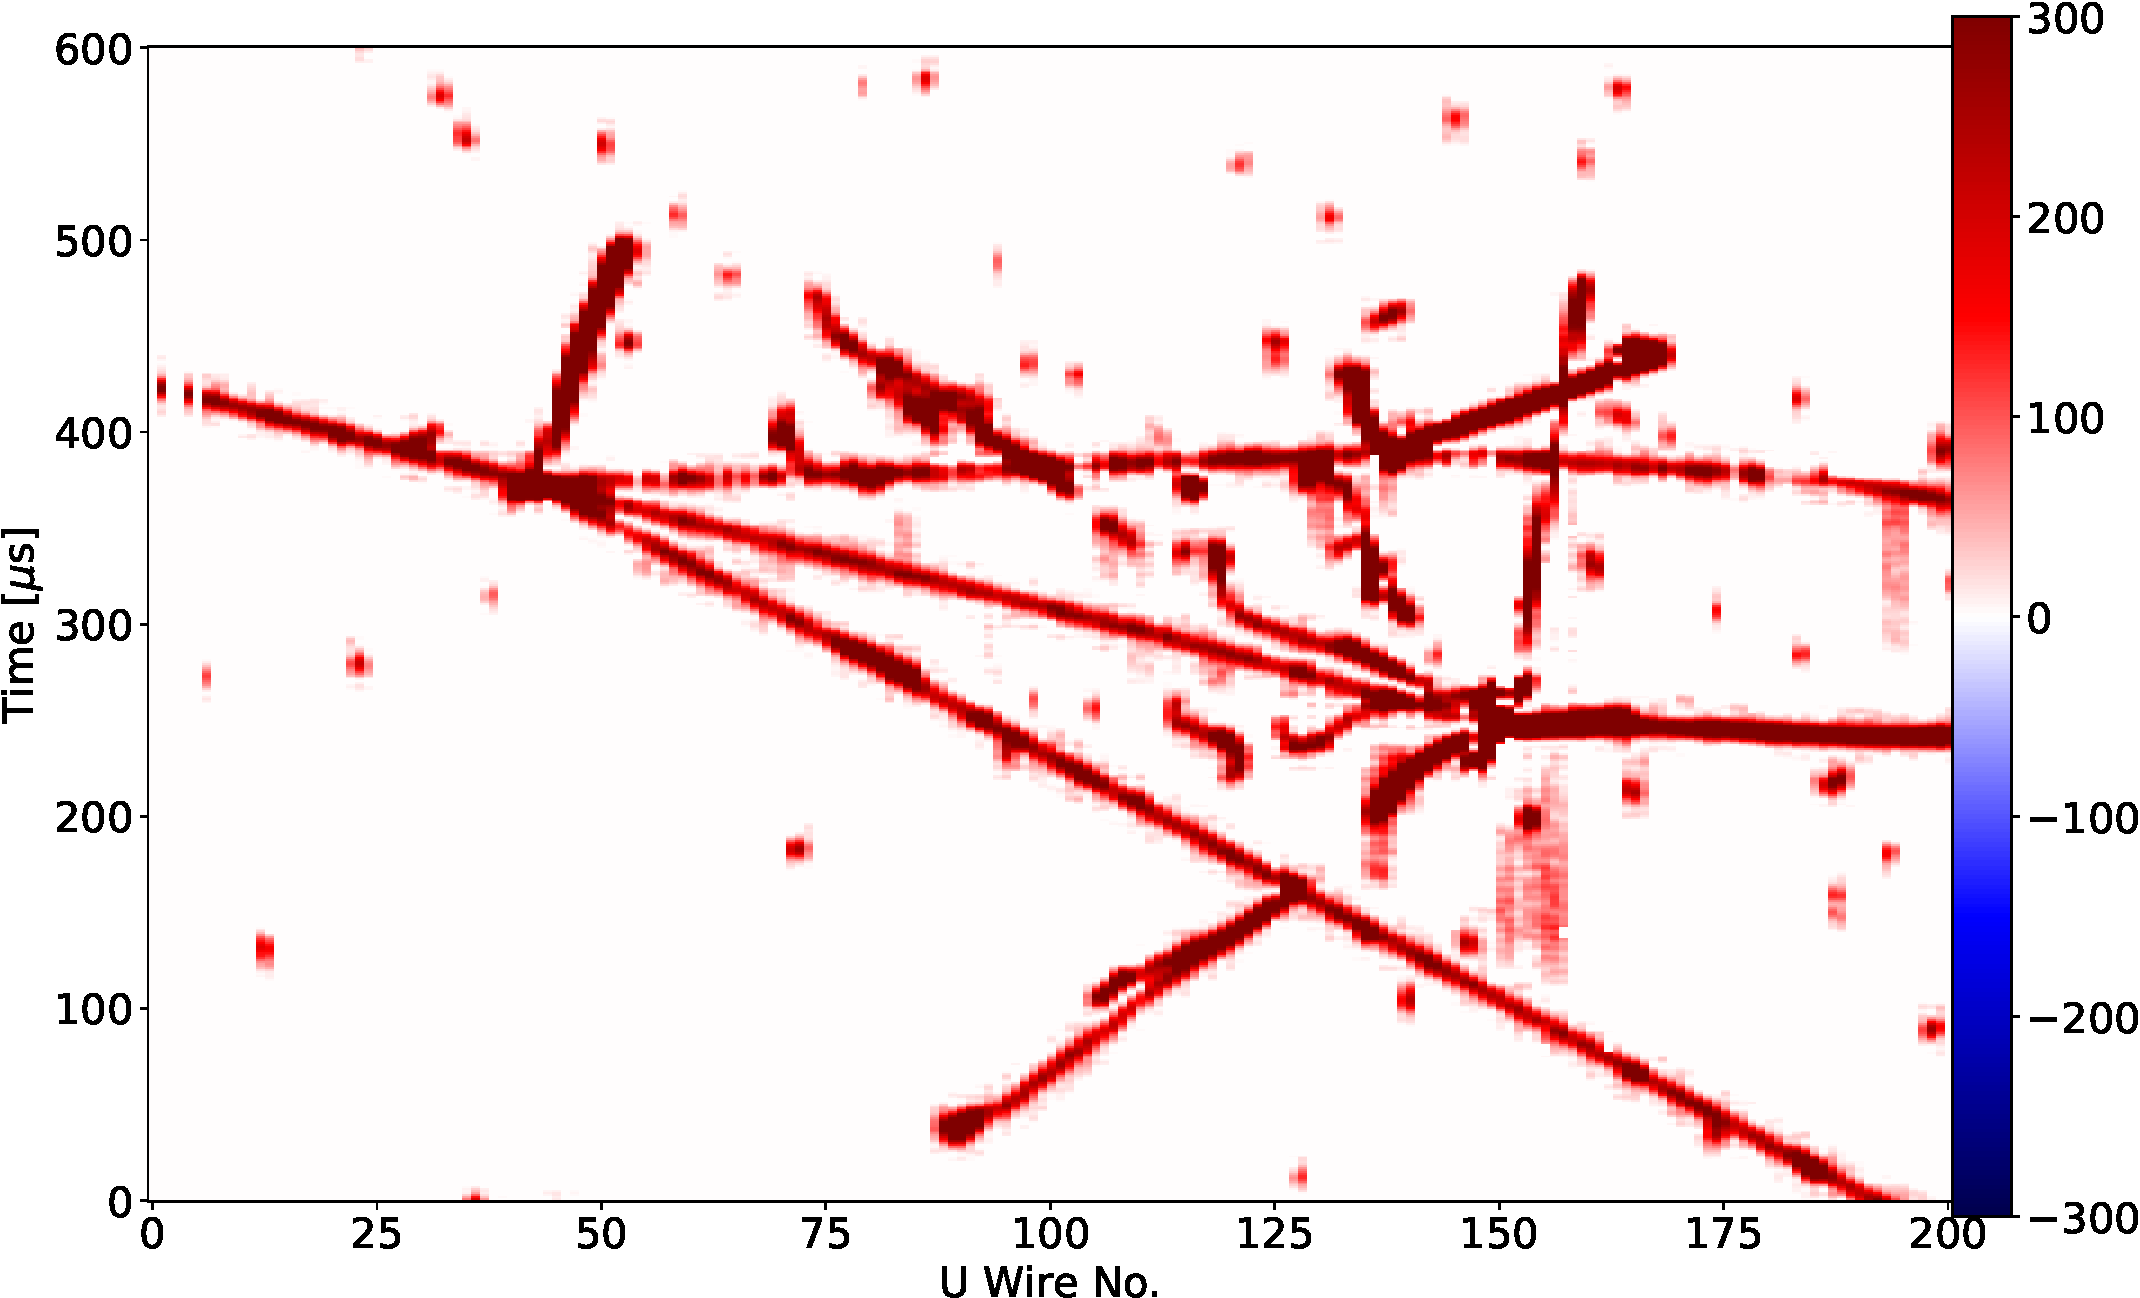
\includegraphics[width=\textwidth]{figures/protodune_evd_decon.pdf}
		\label{fig:pdsp_deconv}
		\caption{After 2D deconvolution.}
	\end{subfigure}

	\caption
	[Example of noise filtering and 2D deconvolution in \protodune{} data.]
	{Example of noise filtering and 2D deconvolution in \protodune{} data. Each
	image shows an example of the wire vs time signals from a region in the
	U--plane, which is an induction plane. Figures from \cite{protoduneperf}.}

	\label{fig:2d_deconv}

\end{figure}

Once the deconvoluted waveforms have been calculated, regions of interest (ROI) 
are defined, these are regions of high amplitude in which charge deposition is
likely to have occurred. Reconstructed hits are found within each region of
interest by fitting gaussian peaks to the pulses within the region; most hits
consist of a single gaussian peak, however in busy regions of the detector
multiple gaussian peaks may be used to fit a single pulse. Each reconstructed
hit will have an associated peak time, width, and integral, these objects form
the basic input for the subsequent pattern recognition algorithms. An example of
the reconstructed hits is shown in Figure \ref{fig:gaushit}.

\begin{figure}

	\centering

	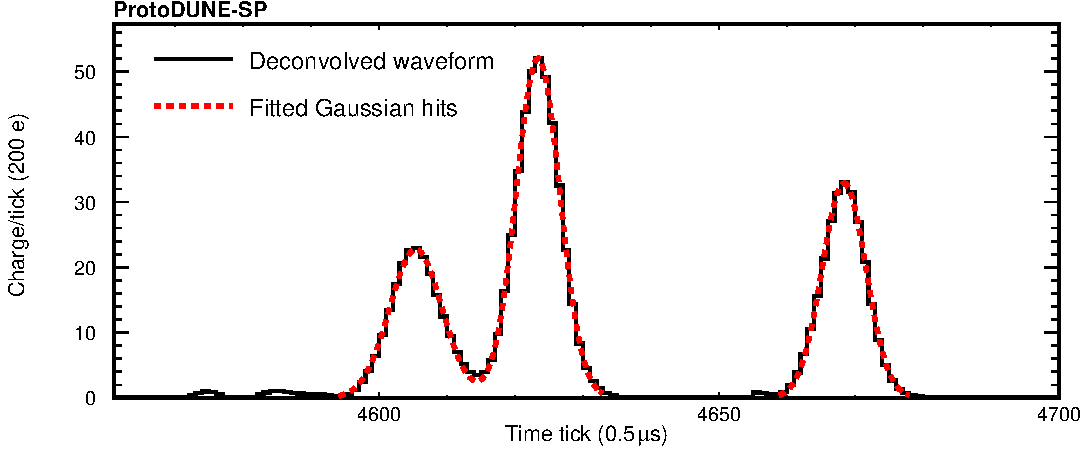
\includegraphics[width=\textwidth]{figures/gaushit.pdf}

	\caption
	[An example of reconstructed hits from \protodune{} data.]
	{An example of reconstructed hits from \protodune{} data. Figure from 
	\cite{protoduneperf}.}

	\label{fig:gaushit}

\end{figure}

Pandora\cite{Marshall2015} is the primary pattern recognition software used in
\protodune{}. It takes a multi--algorithm approach to reconstructing particle
interactions in the detector, and has been successfully used by other LArTPC
detectors, such as MicroBooNE\cite{Acciarri:2017hat}. Pandora handles the 
clustering of hits into 2D clusters, the matching of 2D clusters into 3D
clusters, as well as the reconstruction of 3D objects like tracks and 
showers. Ultimately Pandora returns a tree of reconstructed particle flow
particles (PFParticles), each corresponding to a distinct track or shower, and 
connected through parent--daughter relationships, which define the particle flow
in the interaction. Pandora reconstruction consists of two stages: a cosmic 
pass and a beam pass. 


First the cosmic pass reconstructs the event with algorithms designed to 
reconstruct track--like particles. Track stitching algorithms are used to
predict the true interaction time for certain tracks during this stage. Any 
track which crosses either a CPA or APA will produce track segments on either 
side of the boundary. These segments point in the same direction, but will 
have been displaced from each other in the drift direction based on the 
arrival time of the corresponding particle. The $t_0$ for that track is equal 
to half the time shift required to realign the two segments into a continuous 
track, a visual representation of this algorithm is show in Figure 
\ref{fig:track_stitching}.  After the cosmic pass, any clear cosmic--ray 
candidates are removed under the following conditions\cite{protoduneperf}:
\begin{itemize}
	\item The particle travels through both the top and bottom of the detector.
	\item The assigned $t_0$ is inconsistent with the beam time.
	\item If no $t_0$ assigned, try $t_0 = 0$. If any hits are reconstructed 
		with positions outside of the detector this track is inconsistent with the 
		beam time.
\end{itemize}

\begin{figure}
	\centering
	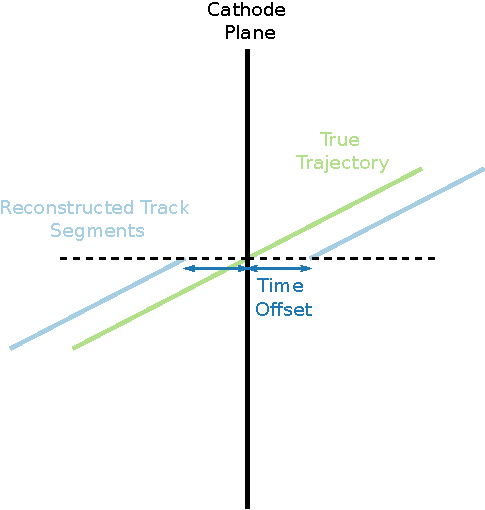
\includegraphics[width=0.6\textwidth]{figures/track_stitch.pdf}
	\caption
	[Diagram demonstrating the track stitching algorithm in \protodune{}.]
	{Diagram demonstrating the track stitching algorithm in \protodune{}. The
	track is initially reconstructed in two segments on either side of the cathode
	plane, which are offset by a distance proportional to the arrival time of the
	track. The two segments can be stitched together by correcting for the time
	offset, resulting in a single track, which has an associated reconstructed
	time based on the time offset.}
	\label{fig:track_stitching}
\end{figure}

Beam particle reconstruction considers only the hits that were not removed by 
being labelled as clear cosmic--rays. These hits are formed into 3D slices which
contain all the hits from a single parent particle and it's daughters. The
slices are reconstructed with both the cosmic--ray and beam particle
algorithms, and a boosted decision tree is used to determine whether a 
given slice is consistent with being a beam particle\cite{protoduneperf}. 

% TODO: define slice
The beam particle reconstruction uses a more complex chain of algorithms
to reconstruct a given slice. These algorithms are capable of reconstructing 
the particle hierarchies seen in the complex hadronic interactions from the 
\protodune{} beam. These algorithms return the particle flow of the 
interactions in the form of PFParticles as well as the reconstructed 
interaction vertex for the primary beam particle. An example of the 
reconstructed particle hierarchy from a \protodune{} beam event is shown in 
Figure \ref{fig:pandora_pfp}.

\begin{figure}

	\centering

	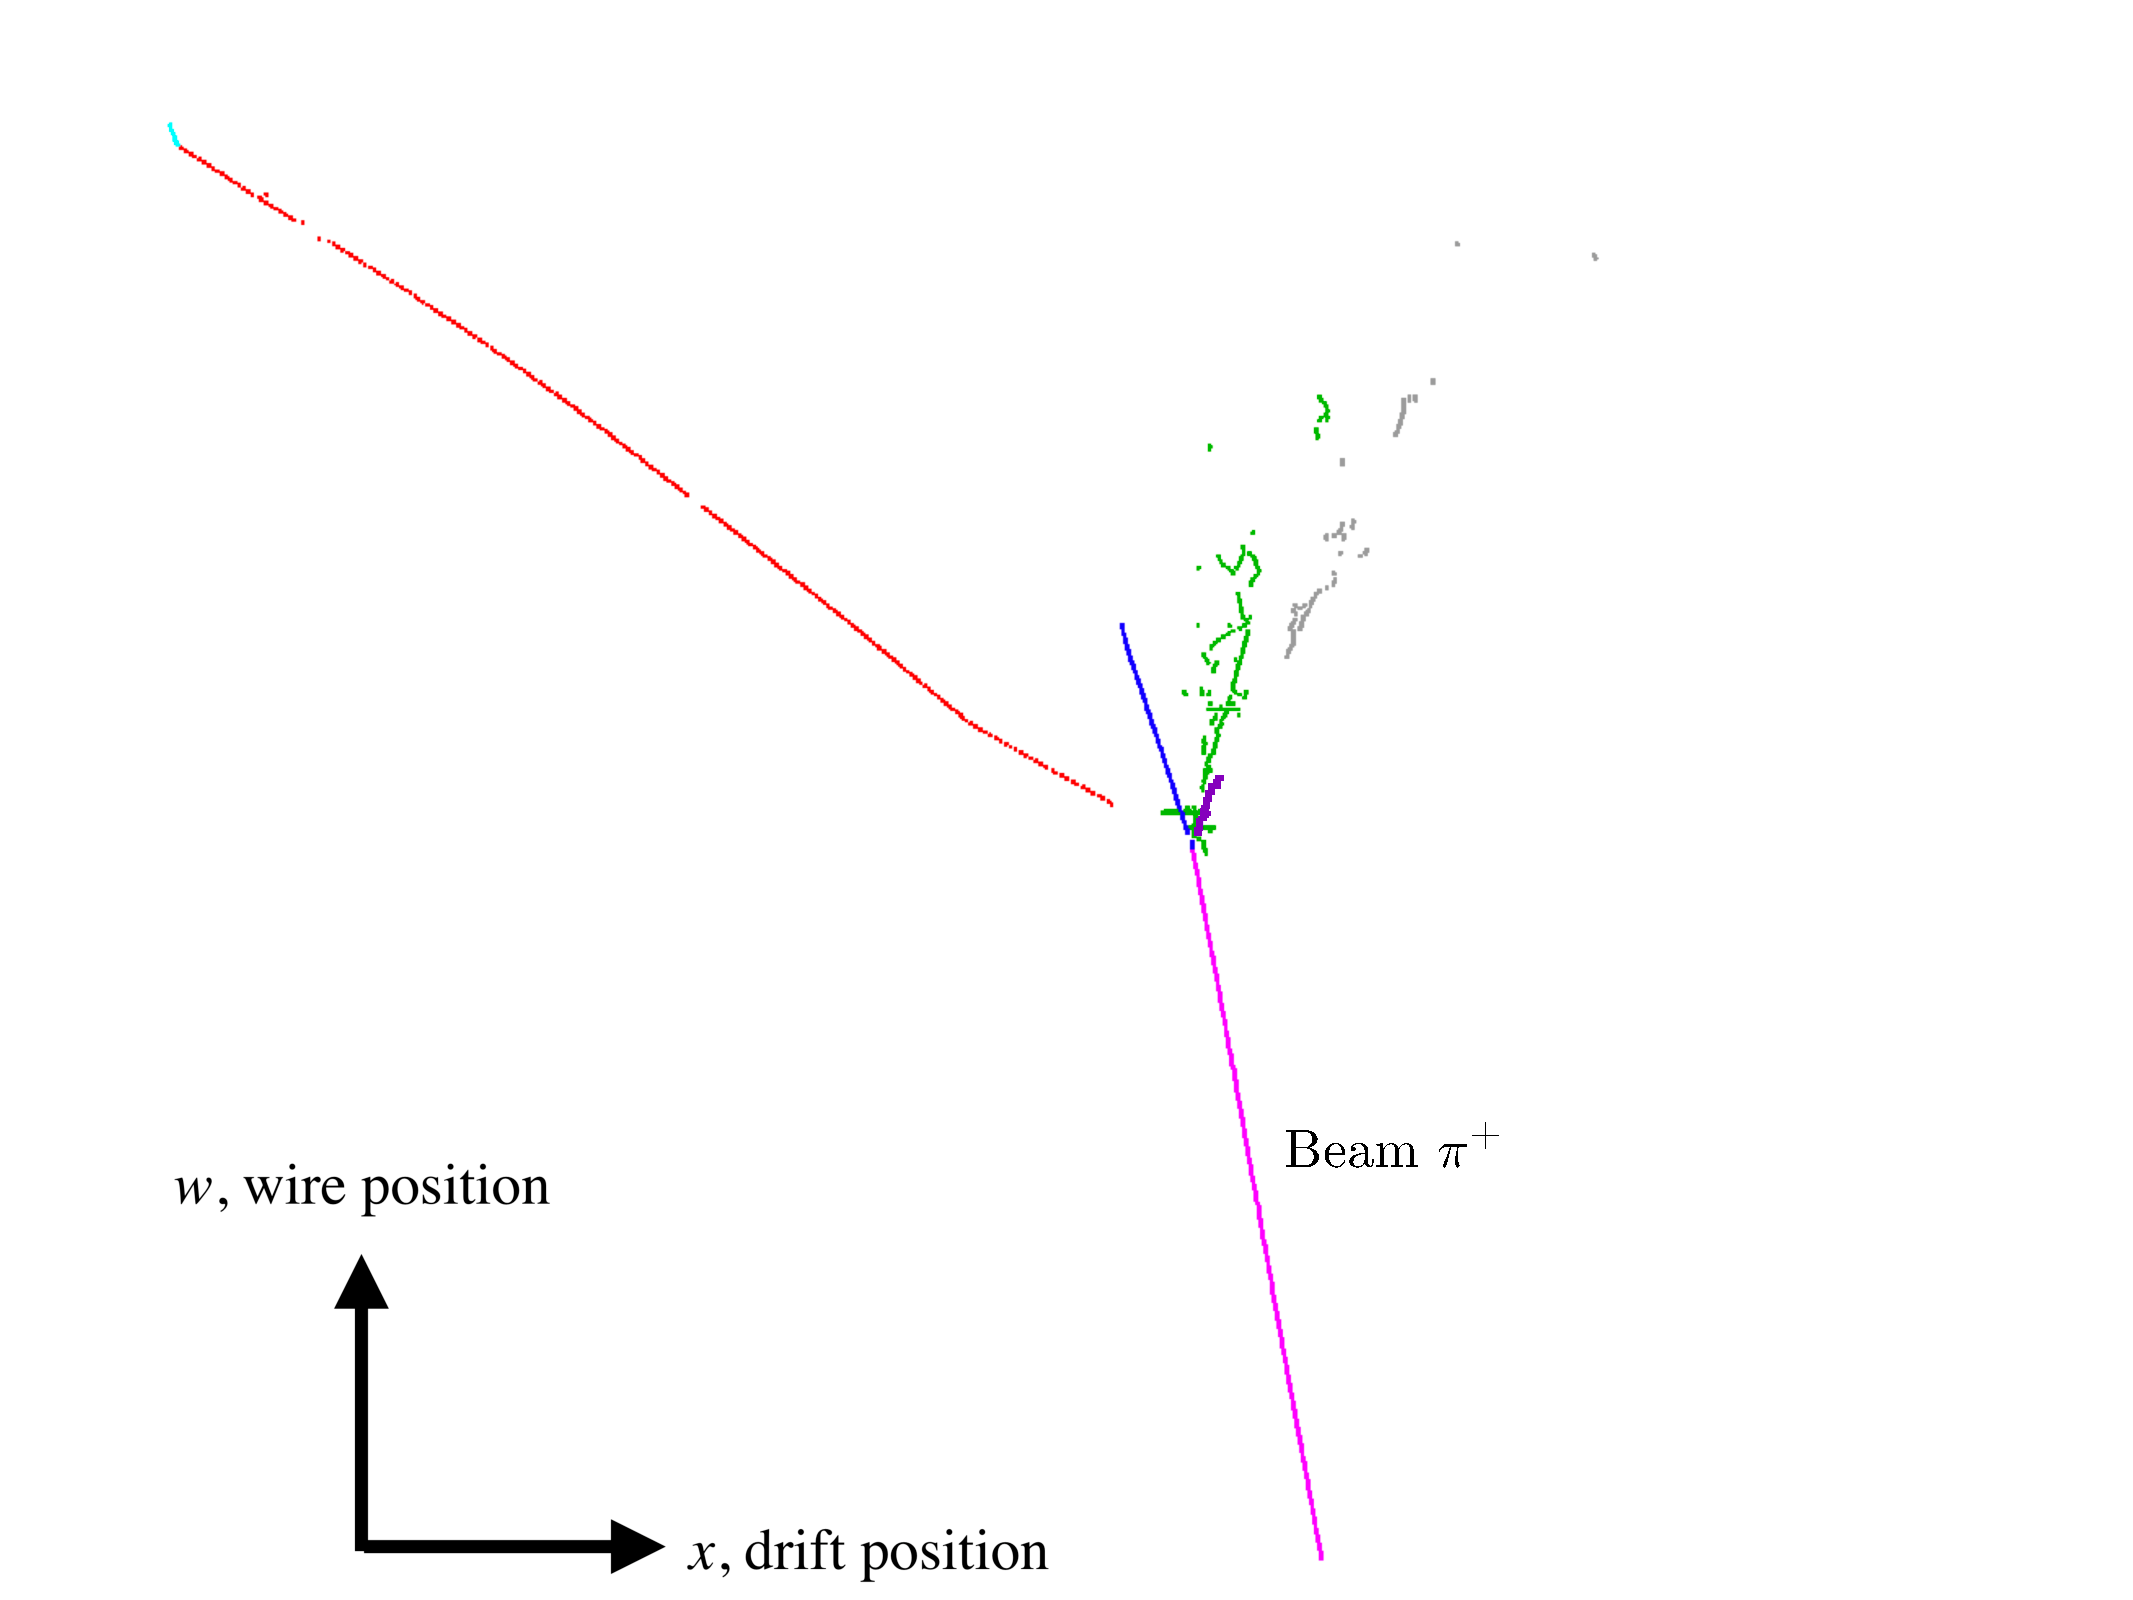
\includegraphics[width=0.9\textwidth]{figures/pandoraEvent.pdf}

	\caption
	[An example of a reconstructed particle hierarchy from Pandora.]
	{An example of a reconstructed particle hierarchy from Pandora, for a beam
	$\pi^+$ event in \protodune{} simulation. The 2D representation is in terms 
	of the wire position and drift position in the collection plane. Each 
	reconstructed particle is labelled in a different colour, demonstrating the 
	reconstructed particle hierarchy of the interaction. Figure from 
	\cite{protoduneperf}.}

	\label{fig:pandora_pfp}

\end{figure}

As well as precise spatial reconstruction, LArTPCs provide excellent
calorimetric information. Each reconstructed hit has an associated charge, 
$Q$, and energy, $E$, which measure the amount of energy deposited by the 
charged particle in that small energy depositon. The measured charge in ADC 
depends on the spatial location of the hit within the TPC, as well as the 
local ionisation density, or $dQ/dx$, in the region of the associated energy 
deposition.  Therefore, to convert the measured charge of each hit into a 
reconstructed energy, a number of spatial and $dQ/dx$ dependent factors need 
to be taken into account.  The reconstructed charge of each hit is given by 
the integrated area under the gaussian fit to that hit. The $dx$ for each hit 
varies based on the direction of the track with respect to the wires, it is 
equal to the wire spacing divided by the sine of the angle between the wire 
and the 2D projection of the track onto the anode plane.

A number of factors affect the measured $dQ/dx$, these effects need to be 
corrected in order to recover the $dQ/dx$ at the source of the ionisation. 
These factors are split into two parts in the \protodune{} reconstruction:
\begin{itemize}
	\item Corrections in the drift direction, X corrections. Examples include 
		longitudinal diffusion, attenuation on impurities, and drift velocity
		variations.
	\item Corrections in the direction of the wire planes, YZ corrections.
		Examples include wire to wire response variations, and transverse diffusion.
\end{itemize}
Calibration factors are calculated for both sets of corrections by considering a
sample of cathode crossing muons. The aim of these calibration matrices is to 
normalise the response over the TPC volume based on the median of the measured
$dQ/dx$ distribution in each location. The distribution is then normalised to 
the average value at the anode plane, where the effects of the X corrections are
expected to be negligible. The corrected $dQ/dx$ is given by
\begin{equation*}
	\left( dQ/dx \right)_{corr} = N_Q \; C_{yz}(y, z) \; C_x(x) \; \left( dQ/dx
	\right)_{reco},
\end{equation*}
where $N_Q$ normalises the median of the distributions to the median value at
the anode, and $C_{yz}$ and $C_{x}$ are the calibration factors for the YZ and 
X corrections respectively.

The final step in energy reconstruction is to convert the corrected $dQ/dx$ into
a reconstructed $dE/dx$, this involves accounting for electron--ion
recombination at the source. The modified box model is used to simulate the
recombination correction, this model has been studied in a LArTPC by the 
ArgoNeuT experiment\cite{Acciarri2013a}. The reconstructed $dE/dx$ is 
\begin{equation*}
	\frac{dE}{dx} = \left( \exp \left( \frac{\frac{dQ}{dx}}{C_{cal}} \frac{\beta^\prime
	W_{ion}}{\rho \epsilon} \right) - \alpha \right)
	\left( \frac{\rho \epsilon}{\beta^\prime} \right)
\end{equation*}
where $C_{cal}$ is a calibration constant used to convert ADC to electrons,
$W_{ion}$ is the work function of argon, $\epsilon$ is the local electric field,
$\rho$ is the liquid argon density, and \(\alpha = 0.93\) and 
\(\beta^\prime = 0.212 \mbox{ (kV/cm)(g/cm}^3) / \mbox{MeV}\) are the box model 
parameters as measured by ArgoNeuT. The calibration constant, $C_{cal}$ is 
calculated by fitting the most probable value of the reconstructed $dE/dx$ 
distribution as a function of range to the theoretical prediction for $dE/dx$ 
vs range for a sample of stopping muons, as shown in Figure \ref{fig:dedx_v_rr}.

\begin{figure}

	\centering

	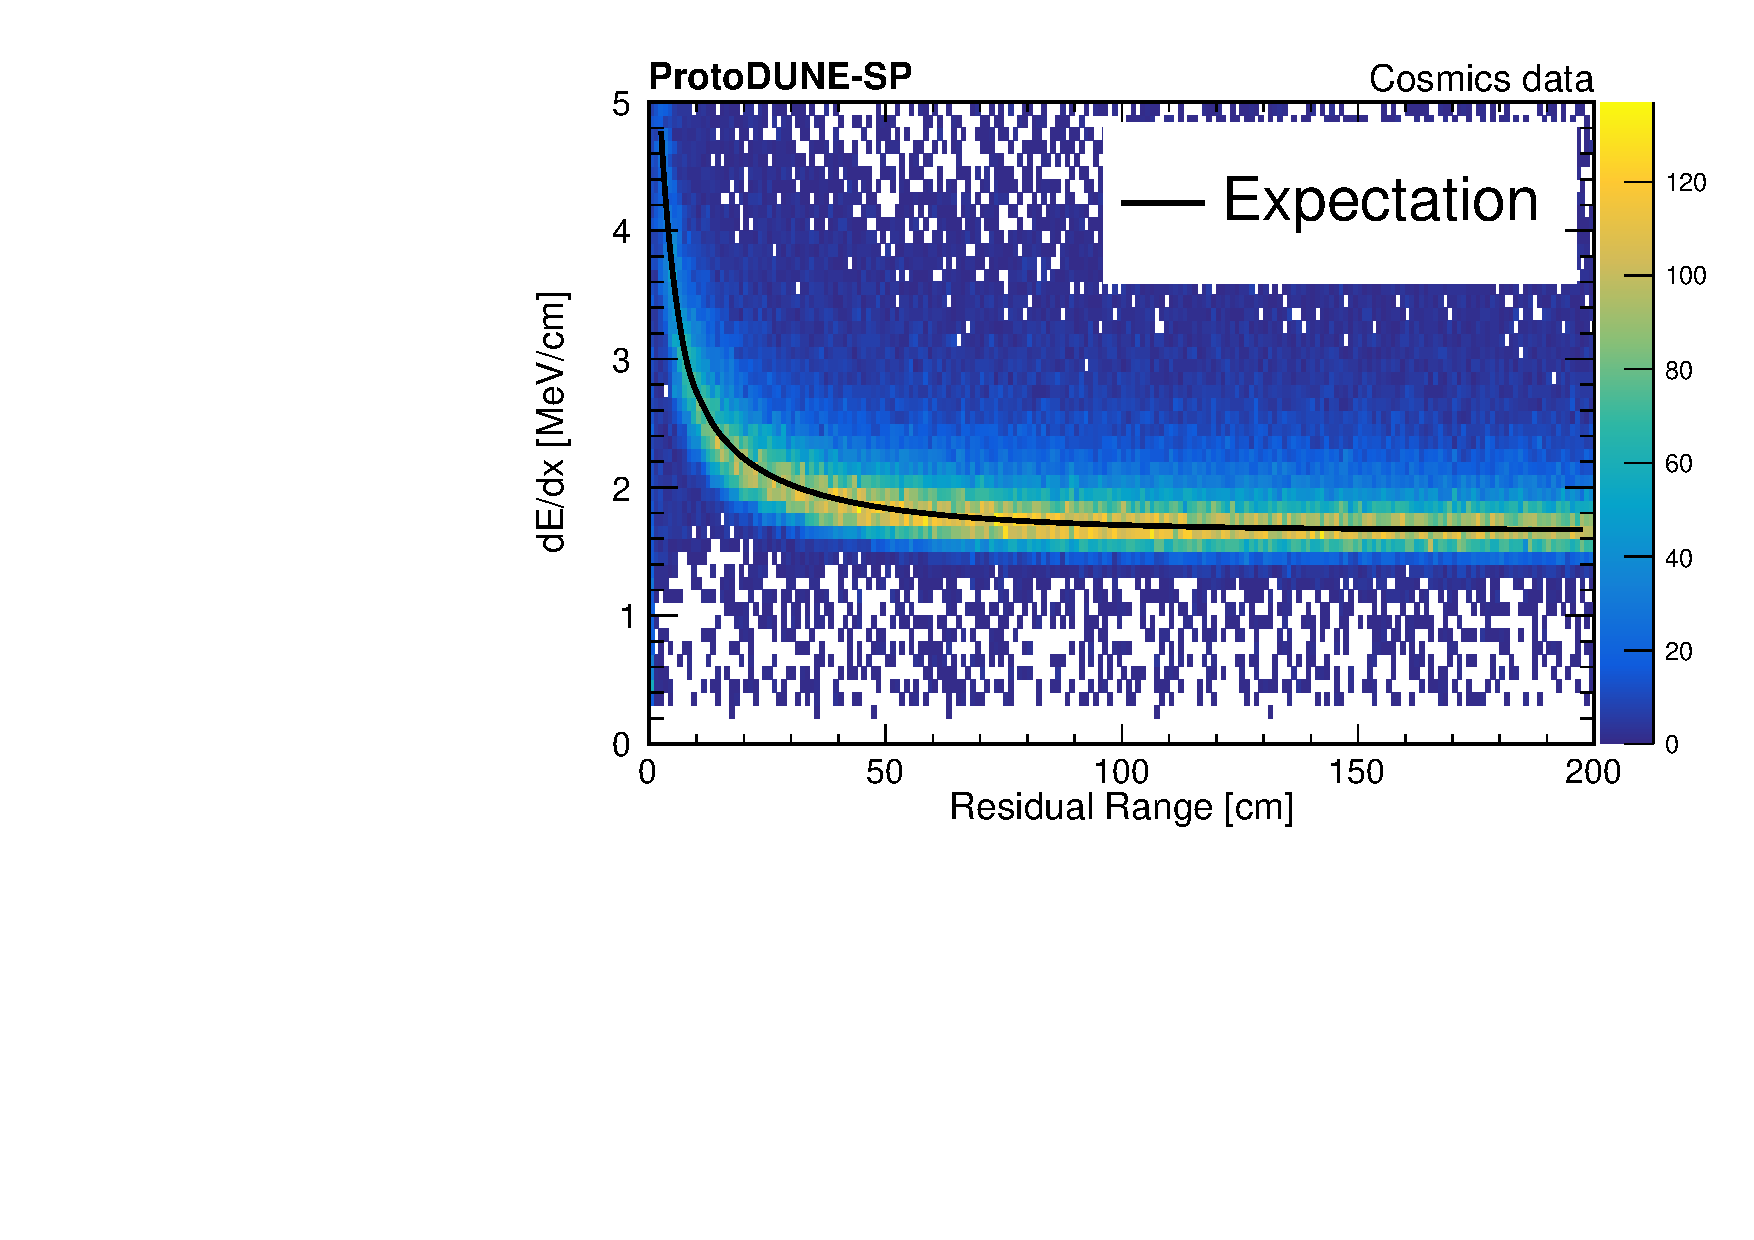
\includegraphics[width=0.9\textwidth]{figures/dedx_v_rr.pdf}

	\caption
	[$dE/dx$ vs residual range for a stopping muon sample in \protodune{} data.]
	{$dE/dx$ vs residual range for a stopping muon sample in \protodune{} data.
	The coloured histogram represents the reconstructed $dE/dx$ in \protodune{}
	data, and the black line is the most probable value of the theoretical 
	distribution. Figure from \cite{protoduneperf}.}

	\label{fig:dedx_v_rr}

\end{figure}

\section{ProtoDUNE--SP Online Monitoring System} \label{sec:pdsp_om}

As well as monitoring the stability of the detector and DAQ systems, the quality
of the collected data has to be constantly monitored. This ensures that data
quality issues are quickly identified, and prevents long runs of low quality
data being collected. The online monitoring system (OM) is responsible for 
providing this quality assurance.

As shown in Figure \ref{fig:pdsp_daq}, the OM is a part of the \protodune{} DAQ
system. The OM is responsible for processing the data and displaying
the results in the control room as soon as possible after the event was 
triggered. It consists of three main components:
\begin{itemize}
	\item Analysis processes which decode and analyse the raw data from each 
		detector subsystem.
	\item Merging processes which collate monitoring data from each subsystem.
	\item A web interface which displays monitoring data.
\end{itemize}

An overview of the data flow in the OM is shown in Figure \ref{fig:om_flow}. 
Data from the detector is first filtered before being run in any OM processes. 
The data which is passed to the OM processes is then split up and decoded by 
the relevant \emph{RawDecoder}, which reformats the data ready for analysis. A 
number of \emph{Analyser Modules} then make use of this data to make plots, 
which are merged, along with plots from external systems, and sent to a web 
interface to be displayed in the control room. The following sections will 
provide a brief summary of these stages, as well as examples of the plots 
which are produced in the OM.

\begin{figure}
	\centering
	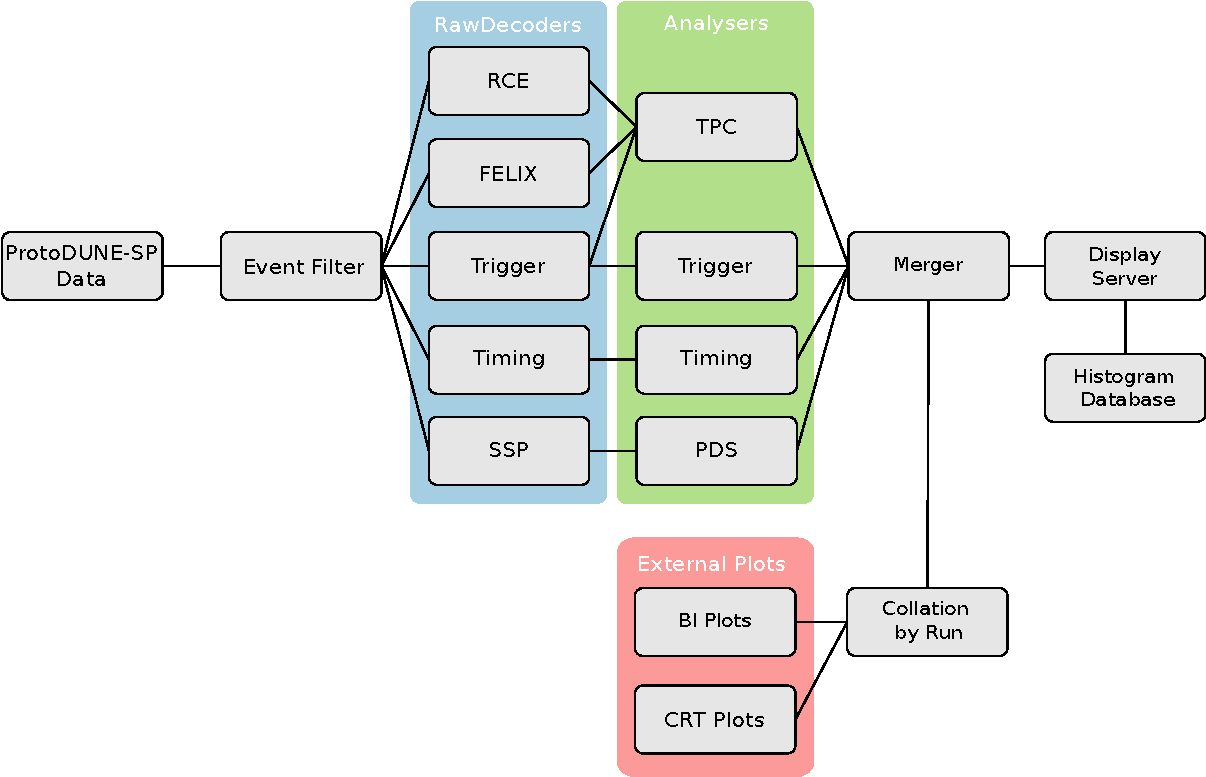
\includegraphics[width=\textwidth]{figures/om_flow.pdf}
	\caption
	[A diagram representing the data flow in the \protodune{} online monitoring system.]
	{A diagram representing the data flow in the \protodune{} online monitoring
	system. The data from each detector subsystem is processed by the RawDecoders
	before being analysed. The results of the analyses are merged, along with data
	from external detector systems, before being sent to the display server to be
	viewed in the control room.}
	\label{fig:om_flow}
\end{figure}

\subsection{Data Processing}
The data processing for the OM is based on Fermilab's Art and ArtDAQ software
frameworks\cite{Green:2012gv, 6495515}, however, the beam instrumentation data 
is analysed outside of the OM system by the CERN beam group. The beam 
instrumentation plots are merged with the rest of the OM plots after data 
processing.

The first step of the data processing is event filtering, the main purpose of
which is to control the flow of data into the OM. Two types of filtering
take place sequentially. First a random filter is used to cut the data rate 
into the OM to a manageable level. This is followed by a second filter, which 
aims to increase the likelihood that processed events were triggered by the 
beam instrumentation or cosmic--ray tagger, as opposed to a random software 
generated trigger. Different OM processes take different amounts of processing 
time per event, therefore, multiple filters are used, to control the data rate 
into each process separately.

After filtering the events are ready to be processed. The data coming into the
OM system is in its raw form. It arrives in small pieces known as
\emph{Fragments}, which have to be decoded before they can be used by the OM. 
The RawDecoders are responsible for interpreting the headers and data streams 
from each detector component, and restructuring the data ready for processing. 
The details of the decoding vary based on the readout system under 
consideration.  Each readout system defines a class, which details the 
contents of each Fragment. The RawDecoders use the contents of this class to 
decode the Fragments in order to prepare the data for 
processing.

After the data has been decoded it is ready to be analysed. This is done by a
number of Analyser Modules, which analyse the data from different detector
components and produce ROOT\cite{ANTCHEVA20092499} plots as output. Details 
of the processing done for each detector component are given below.

\subsubsection*{Time Projection Chamber}
As the largest data source in \protodune{} the TPC data is analysed in several
small steps: basic data checks, pedestals and noise, Fourier analysis, and event
displays. Examples of some of the plots produced by the TPC analysis are
detailed below.

The basic data checks are intended to quickly spot any fundamental issues with
the incoming data. An example of a basic check is to check which FEMBs are
active in the monitored events, Figure \ref{fig:active_femb} shows an example of
the number of events recorded by each FEMB on APA 1 for a sample of 10 analysed
events.

The pedestals and noise are continually evaluated by the online monitoring, this
data is displayed in the control room and used later in the monitoring chain to
flatten the background in the event displays. Basic hit removal is used to 
ensure that the pedestals and root mean square deviation (RMS) are only 
calculated in the regions of the readout corresponding to noise signals. The 
RMS of all channels can be represented on a single plot by arranging the 
channels into a 2D grid and displaying the RMS as the colour scale on a 2D 
histogram, an example of this plot is shown in Figure \ref{fig:ped_noise}.

To identify noise sources in the APA it is useful to study the Fourier transform
of the signal distribution, which allows the noisy frequencies to be identified.
Individual noise sources can be identified by studying the Fourier 
distributions under different operating conditions, for example, the cameras 
in the TPC were identified as a noise source in this way. The OM, therefore, 
provides fast fourier transforms (FFT) for each APA, an example of the FFT for 
a single FEMB is shown in Figure \ref{fig:TPC_FFT}.

\begin{figure}

	\centering

	\begin{subfigure}[b]{0.75\textwidth}
		\centering
		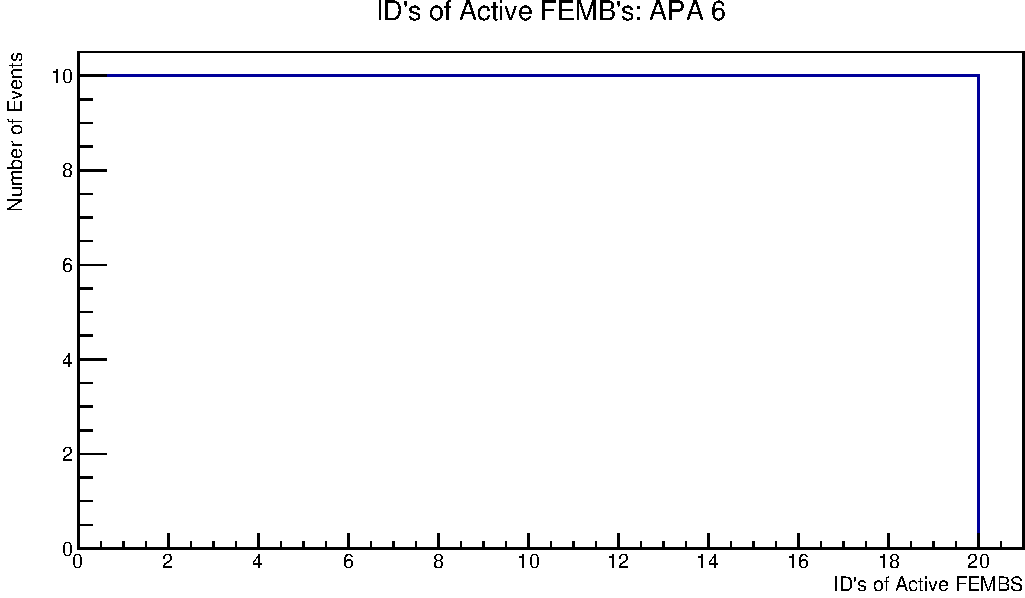
\includegraphics[width=\textwidth]{figures/active_femb.pdf}
		\caption {Number of events recorded by each FEMB on APA 6. 10 events are
		processed for each OM file, therefore, the histogram should be filled to 10
		for every FEMB, if not there has been an issue.}
		\label{fig:active_femb}
	\end{subfigure}

	\begin{subfigure}[b]{0.75\textwidth}
		\centering
		\vspace{3mm}
		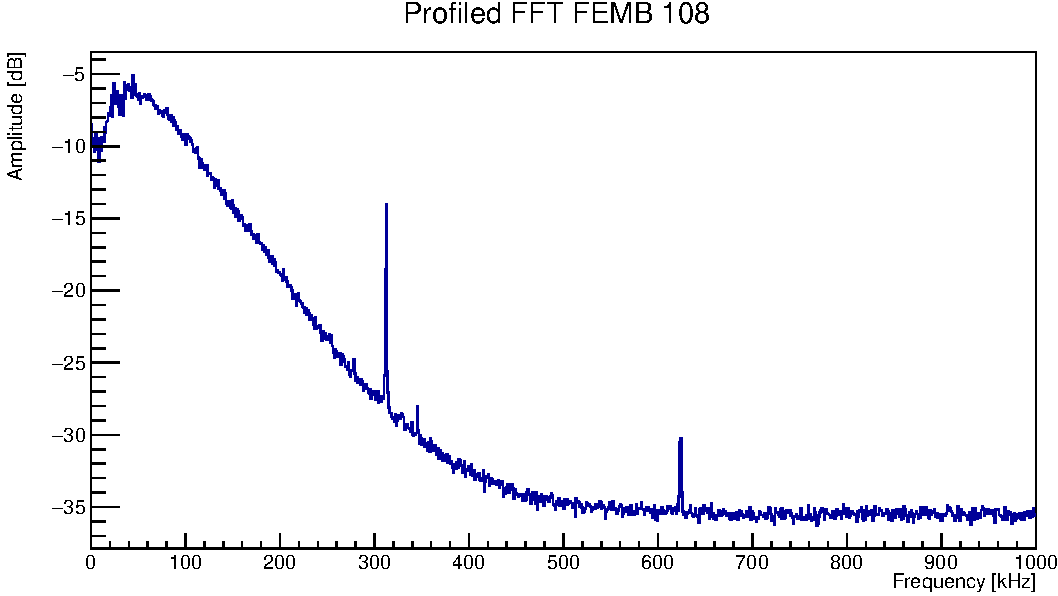
\includegraphics[width=\textwidth]{figures/tpc_fft.pdf}
		\caption {The profiled FFT from all channels from a single FEMB.}
		\label{fig:TPC_FFT}
	\end{subfigure}

	\begin{subfigure}[b]{0.75\textwidth}
		\centering
		\vspace{3mm}
		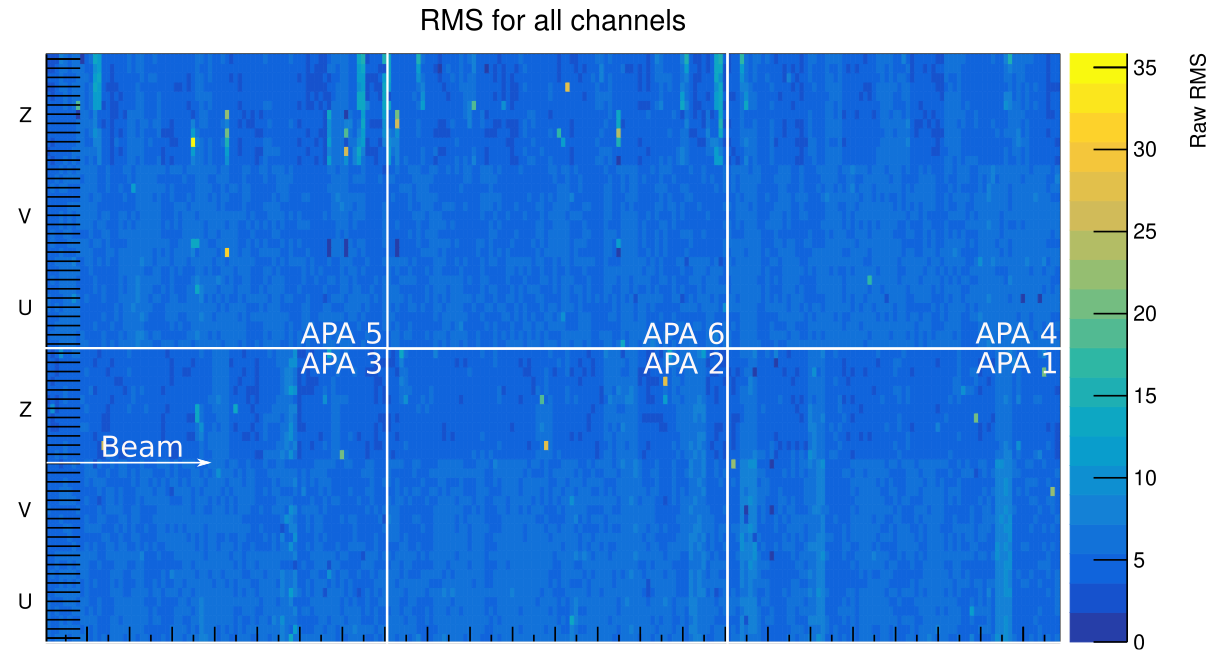
\includegraphics[width=\textwidth]{figures/all_chan_rms.png}
		\caption {RMS for all channels displayed \emph{pseudo--geometrically} on a 
		single histogram. The RMS for every TPC channel is plotted, and the channels 
		are organised by APA and wire plane.} 
		\label{fig:ped_noise}
	\end{subfigure}

	\caption
	[Examples of online monitoring plots for the TPC data.]
	{Examples of online monitoring plots for the TPC data.}
	\label{fig:tpc_om}

\end{figure}

Event displays show all the data from all the TPC readout channels
simultaneously and, as such, they provide the most general check of TPC 
performance in the OM. During the beam run of \protodune{}, a number of issues 
in the data were first identified in the event display, for example, issues in 
the channel mapping and timing synchronisation. They are also particularly 
useful for checking that the beam trigger results in beam particles in the 
TPC. As a result a significant effort was made to make event displays 
available in the \protodune{} OM system. In particular, changes to the display 
server were required, these changes are discussed later in this chapter. 

Event displays were offered for all views in all APAs. In addition, a special 
event display, which focussed on the data in the beam window, and event 
displays, which showed the data from all APAs either side of the TPC as a 
continuous image were produced. The event displays took the longest time to 
process out of all the plots in the OM, therefore, only one set of event 
displays was made per OM output file. To maximise the number of beam particles 
in the event displays, the trigger information was included during 
processing.  An example of a beam--window event display is shown in Figure 
\ref{fig:beam_evd}; the timing synchronisation issue mentioned previously is 
visible here, this issue affects a single FEMB and is mitigated during offline 
reconstruction.  

\begin{figure}

	\centering

	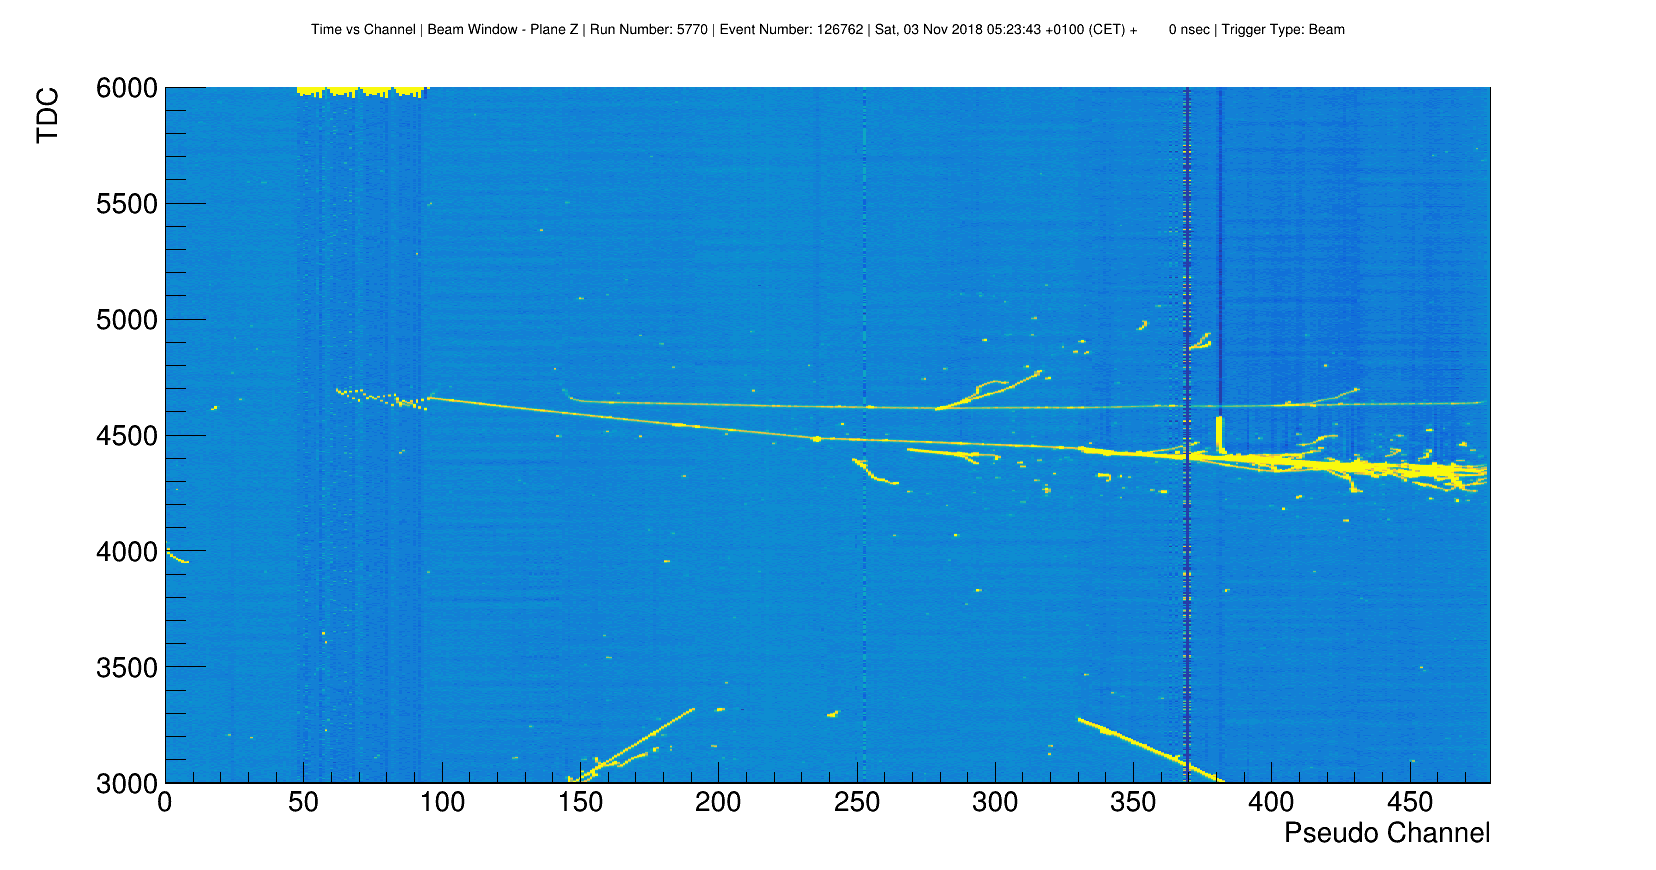
\includegraphics[width=\textwidth]{figures/beam_evd.png}

	\caption
	[An example of a beam window event display from the \protodune{} online
	monitoring system.]
	{An example of a beam window event display from the \protodune{} online
	monitoring system. The measured signal on the collection plane wires in ADC 
	is displayed on wire vs time axes, for the region where the beam enters the 
	TPC. An example of a data defect which was discovered in the OM can be seen 
	on the left side of the plot, this timing issue was mitigated during offline
	reconstruction.}

	\label{fig:beam_evd}

\end{figure}

\subsubsection*{Photon Detection System}
Similarly to the TPC data, the PDS data is analysed for pedestal, RMS, and FFTs;
in addition, the raw waveforms for each channel are accumulated over a number of
events and displayed in the online monitoring. Examples of some of the PDS 
monitoring plots are shown in Figure \ref{fig:pds_om}.

\begin{figure}

	\centering

	\begin{subfigure}[b]{0.8\textwidth}
		\centering
		\vspace{3mm}
		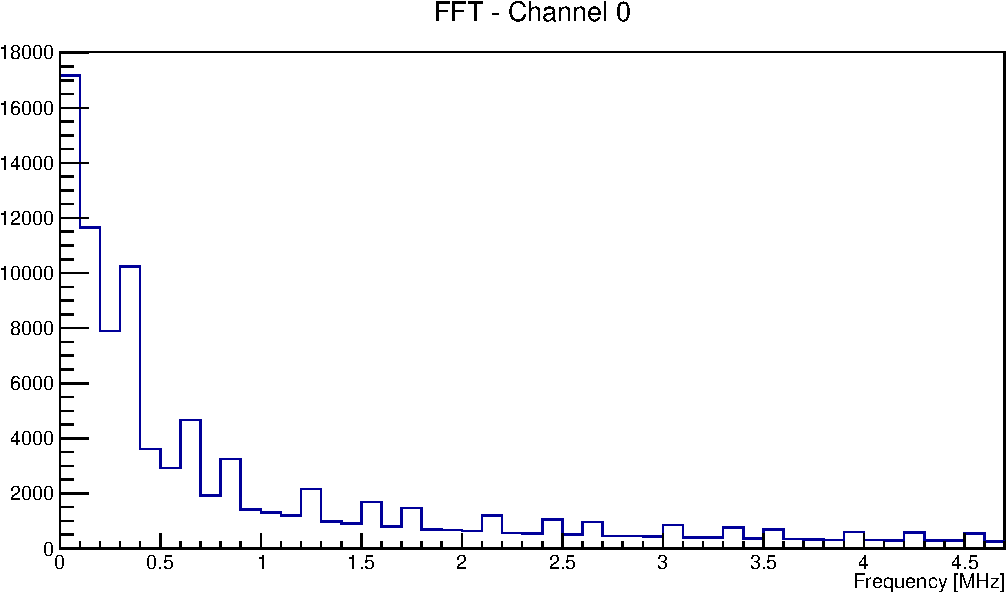
\includegraphics[width=\textwidth]{figures/pds_fft.pdf}
		\caption {FFT for a single PDS channel.}
		\label{fig:PDS_FFT}
	\end{subfigure}

	\begin{subfigure}[b]{0.8\textwidth}
		\centering
		\vspace{3mm}
		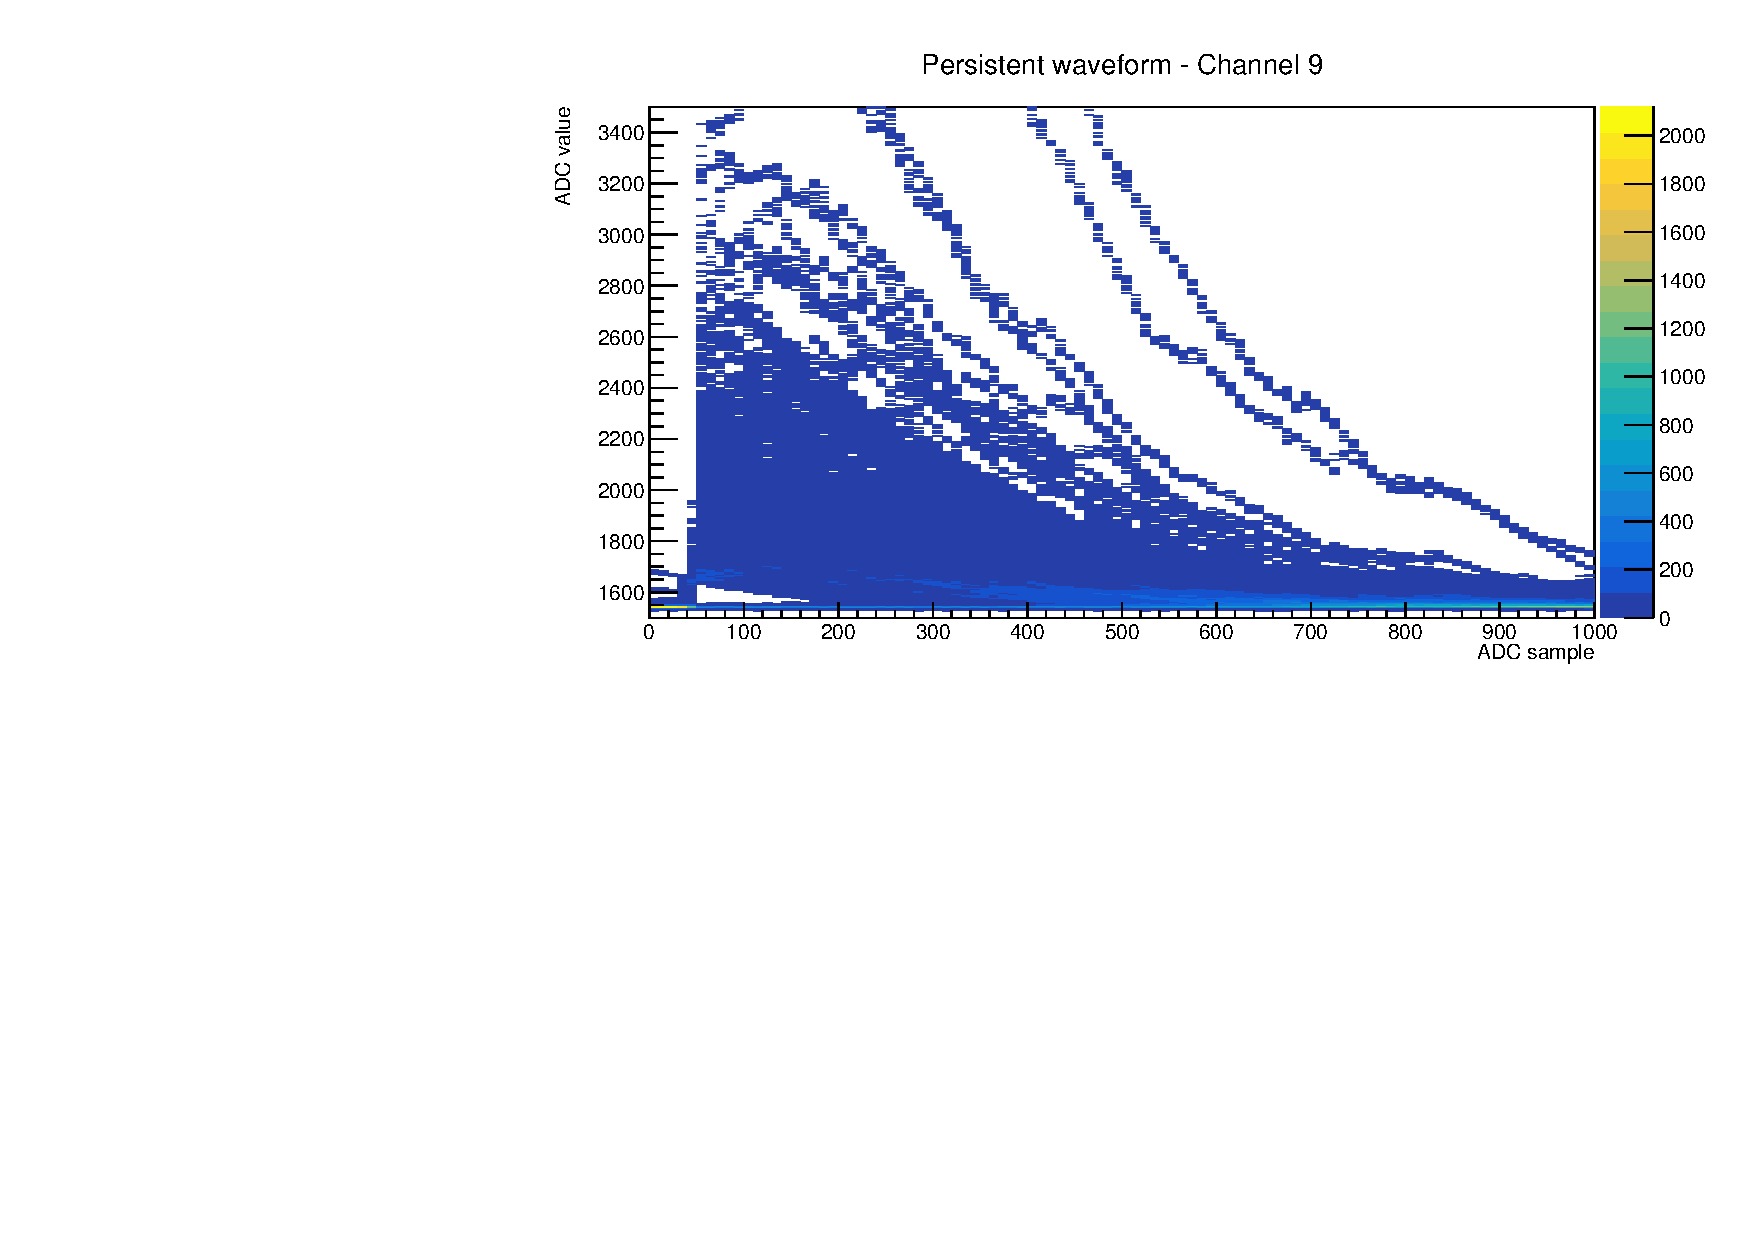
\includegraphics[width=\textwidth]{figures/pds_wav.pdf}
		\caption {Waveforms for a single PDS channel, which have been accumulated
		over a number of events. The ADC value as a function of time sample is shown
		for a number of PDS waveforms from a single channel.}
		\label{fig:PDS_wav}
	\end{subfigure}

	\caption
	[Examples of online monitoring plots for the photon detection system data.]
	{Examples of online monitoring plots for the photon detection system data.}
	\label{fig:pds_om}

\end{figure}

\subsubsection*{Trigger and Timing}
The trigger and timing systems share much of the same data and, therefore, 
their monitoring is related. Some examples of useful timing and trigger plots 
include time--stamp difference distributions, and trigger records. The 
time--stamp delta plots show the difference in time--stamp between consecutive 
events, this distribution can be used to monitor the stability of the trigger 
rate during triggered operation. Trigger records are 2D histograms which 
detail the time and type of trigger issued by the trigger board. Figure 
\ref{fig:timing_OM} contains examples of these two plots.

\begin{figure}

	\centering

	\begin{subfigure}[b]{0.8\textwidth}
		\centering
		\vspace{3mm}
		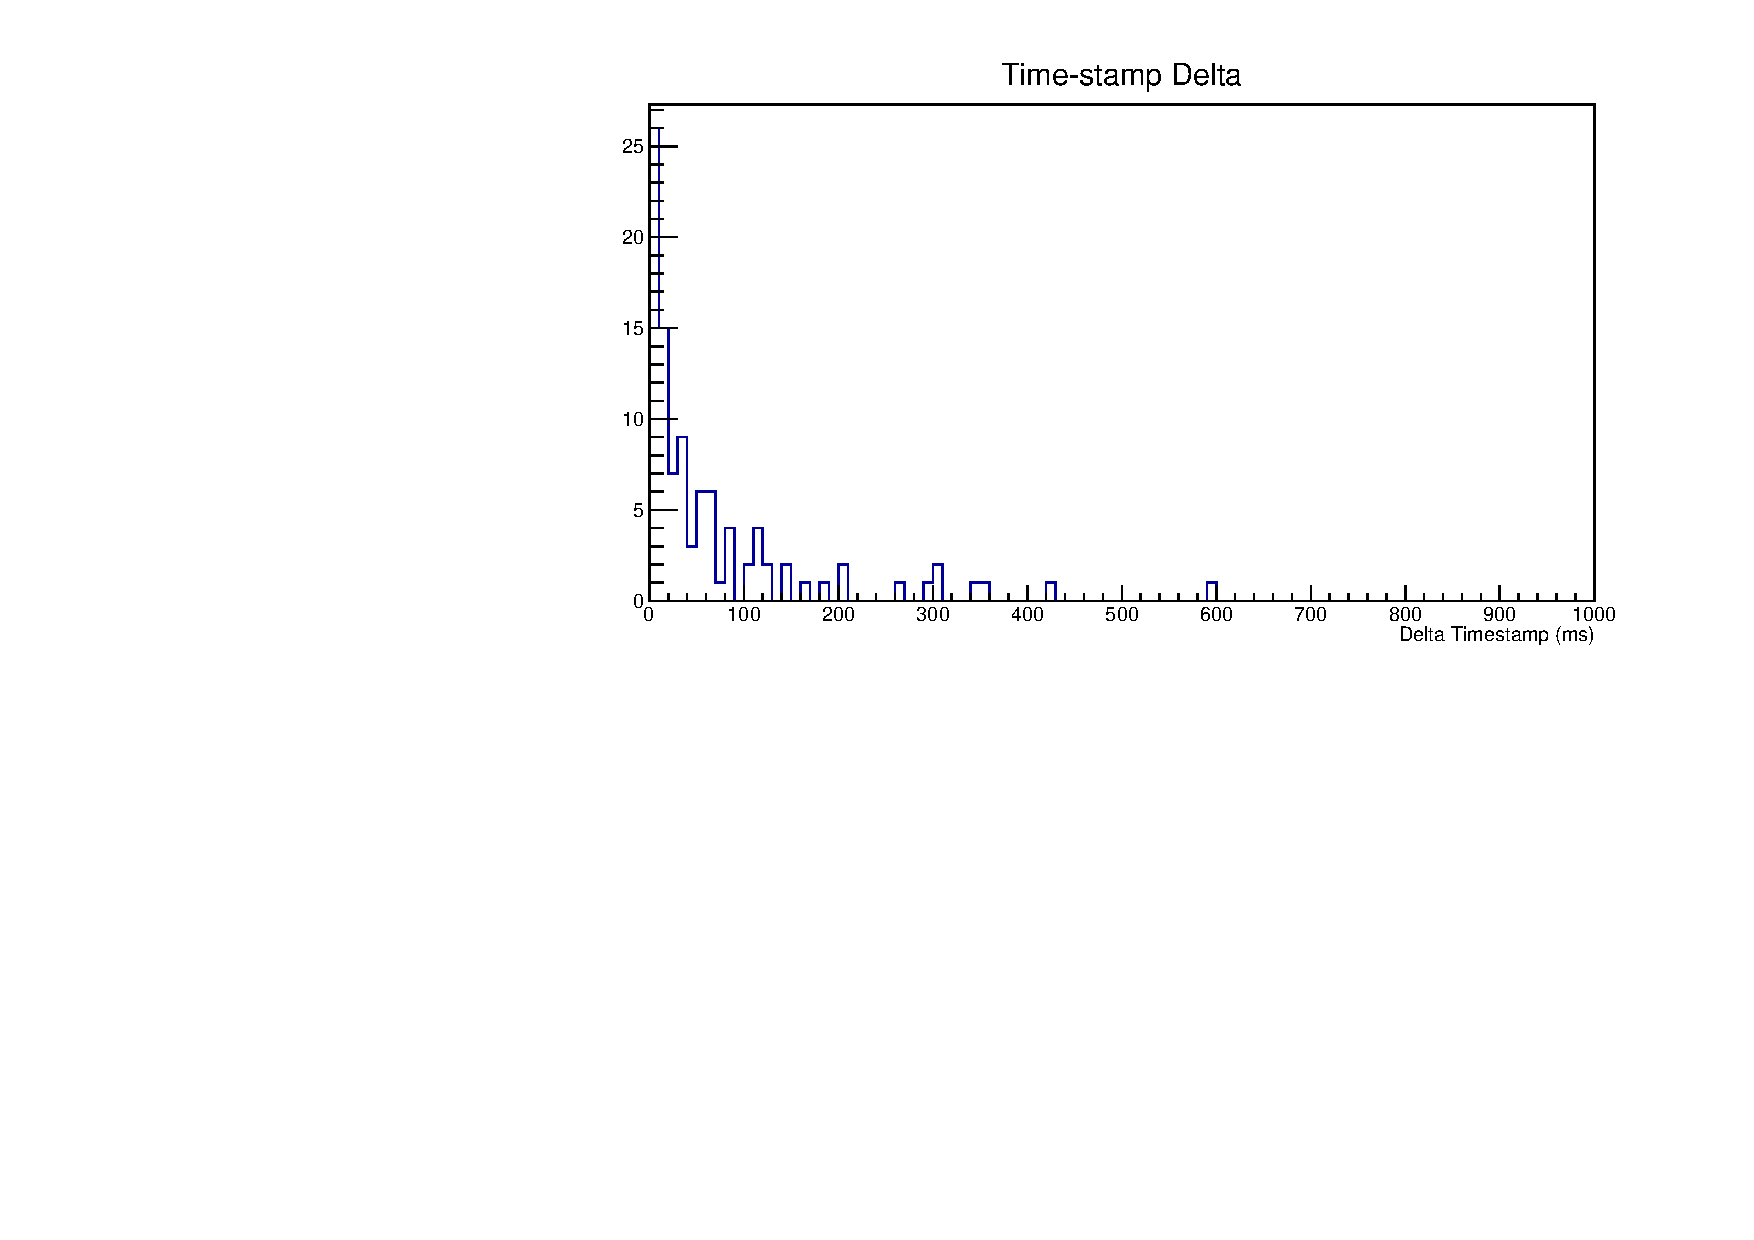
\includegraphics[width=\textwidth]{figures/timestamp_delta.pdf}
		\caption {Time--stamp delta distribution. A histogram of the difference in time
		between subsequent events.}
		\label{fig:timestamp_delta}
	\end{subfigure}

	\begin{subfigure}[b]{0.8\textwidth}
		\centering
		\vspace{3mm}
		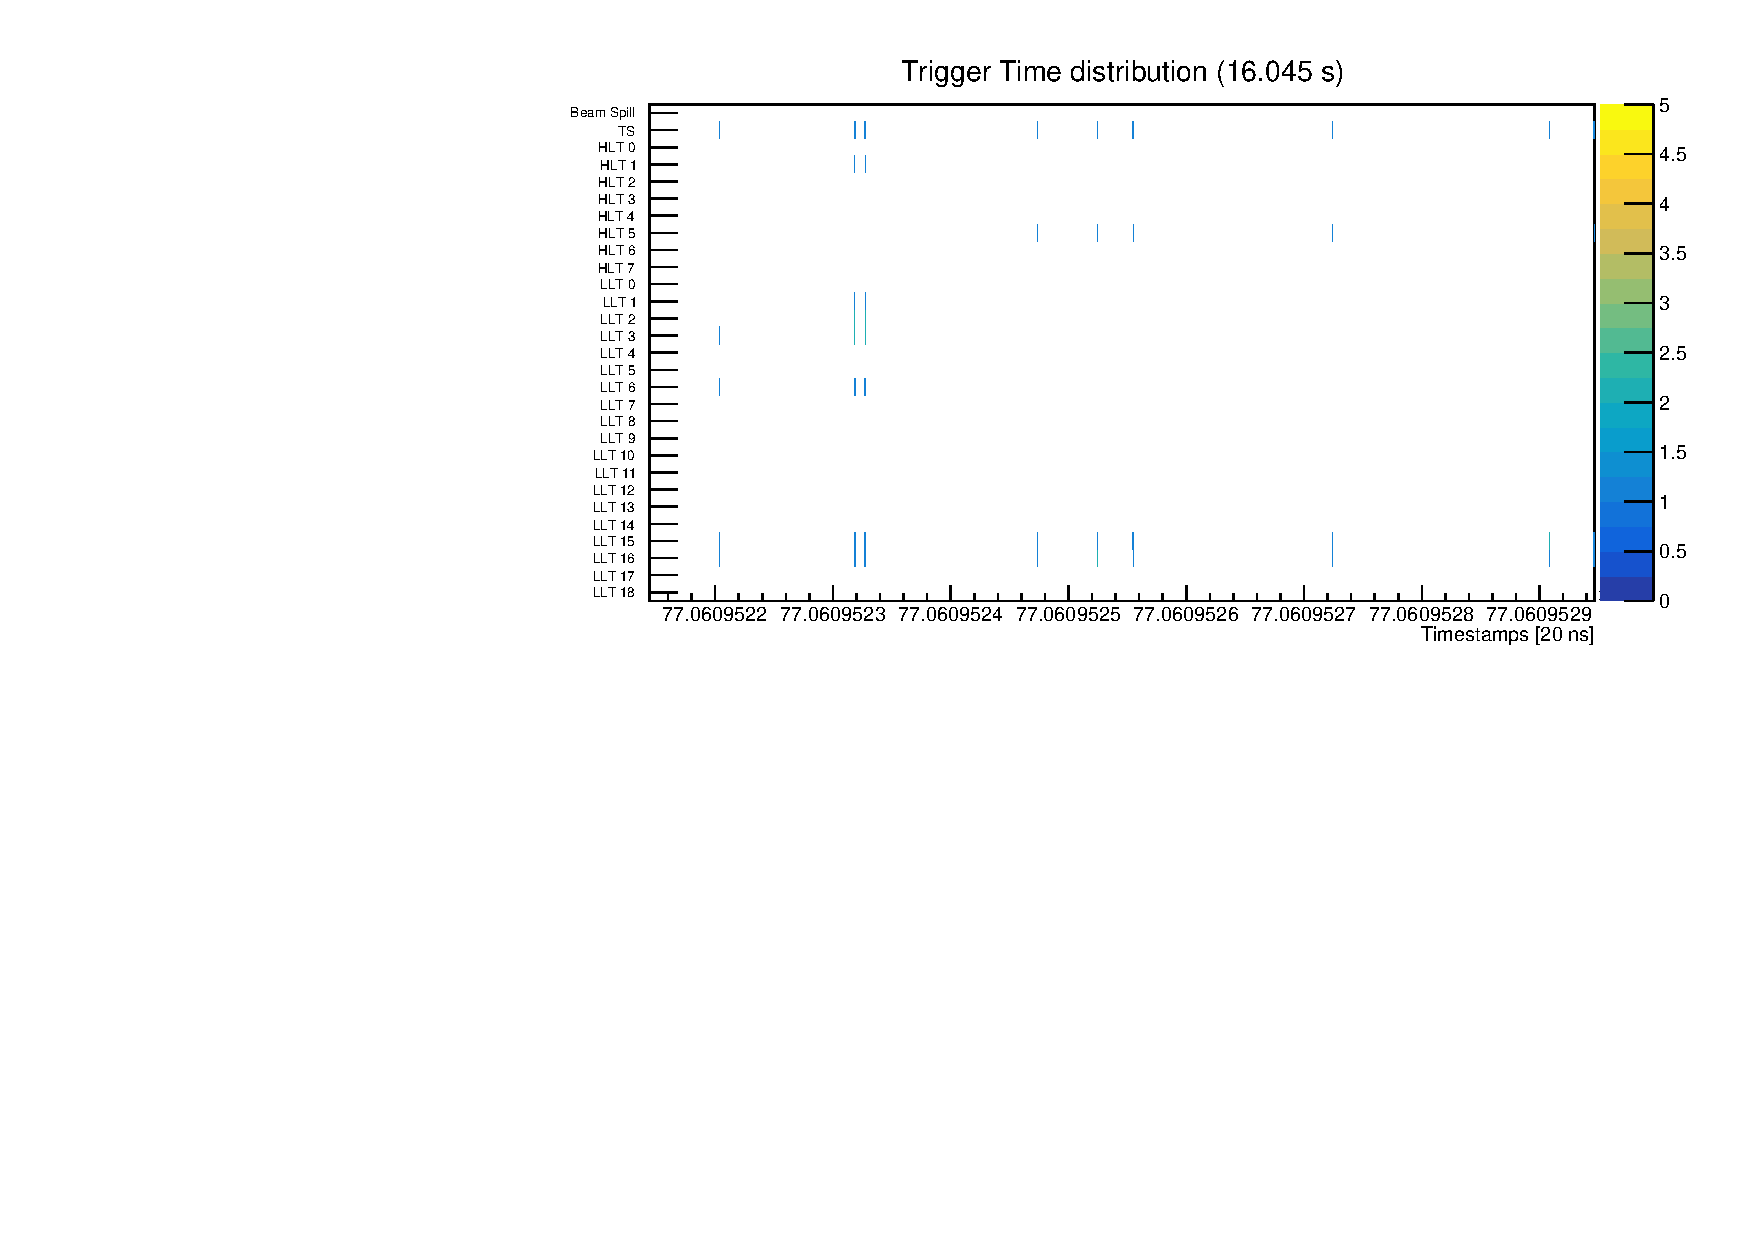
\includegraphics[width=\textwidth]{figures/trigger_record.pdf}
		\caption {Trigger records. A 2D histogram which shows the active trigger
		types as a function of the trigger time--stamp for a number of events.}
		\label{fig:trig_record}
	\end{subfigure}

	\caption
	[Examples of online monitoring plots for the timing and trigger data.]
	{Examples of online monitoring plots for the timing and trigger data.}
	\label{fig:timing_OM}

\end{figure}

\subsubsection*{Beam Instrumentation}
During the \protodune{} beam run, the beamline instrumentation was monitored 
by CERN, who produced beamline monitoring plots\cite{Booth:2019brj}. These plots
were continually overwritten on a time schedule which was decoupled from the 
\protodune{} running schedule, the OM was responsible for collating the output 
of these plots in sync with the \protodune{} run schedule, so that the 
collated beam information for each run could be monitored. After collation the 
beam instrumentation plots were merged with the rest of the OM plots. The beam 
instrumentation plots included momentum, and time of flight, examples of which 
are shown in Figure \ref{fig:beam_OM}.

\begin{figure}

	\centering

	\begin{subfigure}[b]{0.8\textwidth}
		\centering
		\vspace{3mm}
		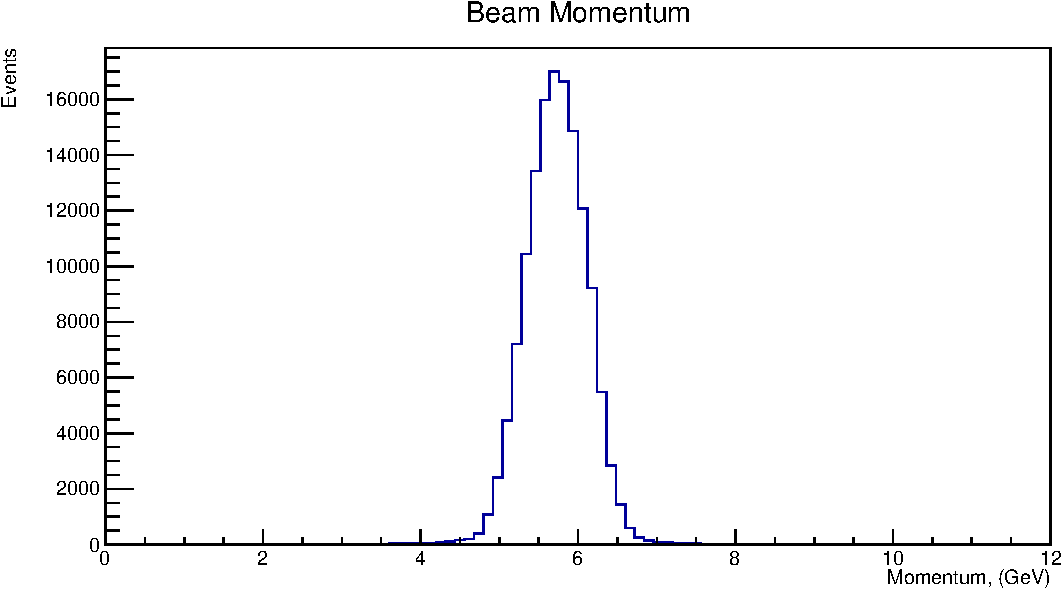
\includegraphics[width=\textwidth]{figures/beam_momentum_om.pdf}
		\caption {Beam momentum distribution.}
		\label{fig:beam_momentum_om}
	\end{subfigure}

	\begin{subfigure}[b]{0.8\textwidth}
		\centering
		\vspace{3mm}
		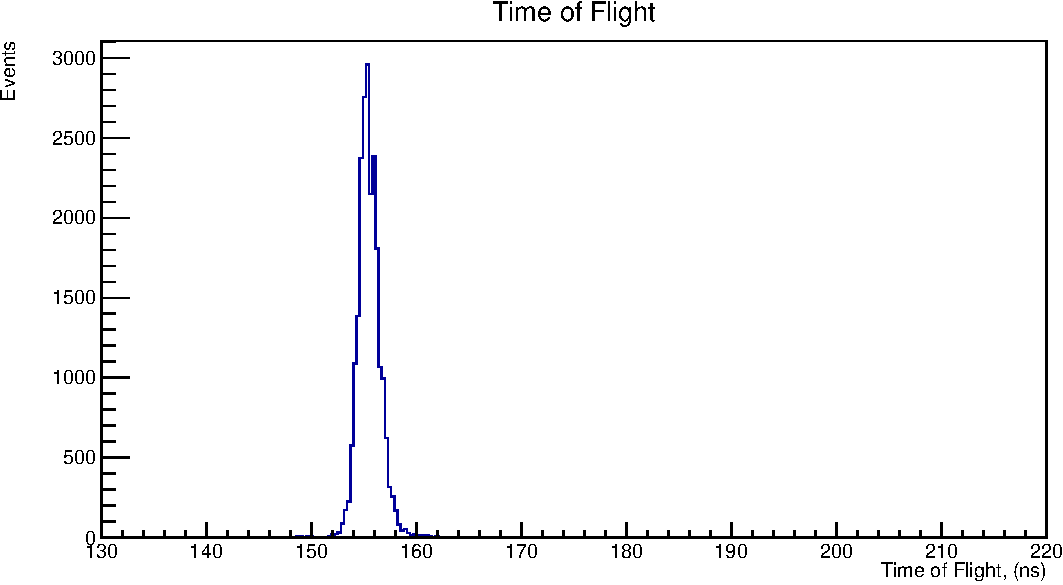
\includegraphics[width=\textwidth]{figures/beam_tof_om.pdf}
		\caption {Beam time of flight distribution.}
		\label{fig:beam_tof_om}
	\end{subfigure}

	\caption
	[Examples of online monitoring plots for the beam instrumentation.]
	{Examples of online monitoring plots for the beam instrumentation.}
	\label{fig:beam_OM}

\end{figure}

\subsubsection*{Cosmic--Ray Tagger}
A bug in the DAQ meant that the CRT was run separately during the main beam 
run. Therefore, the CRT data was analysed separately from the rest of the 
\protodune{} systems and merged in the OM in the same way as the beam 
instrumentation data. Some examples of CRT monitoring plots include the rate 
of hits and the mean ADC for each channel, these are shown in Figure 
\ref{fig:crt_OM}.

\begin{figure}

	\centering

	\begin{subfigure}[b]{0.8\textwidth}
		\centering
		\vspace{3mm}
		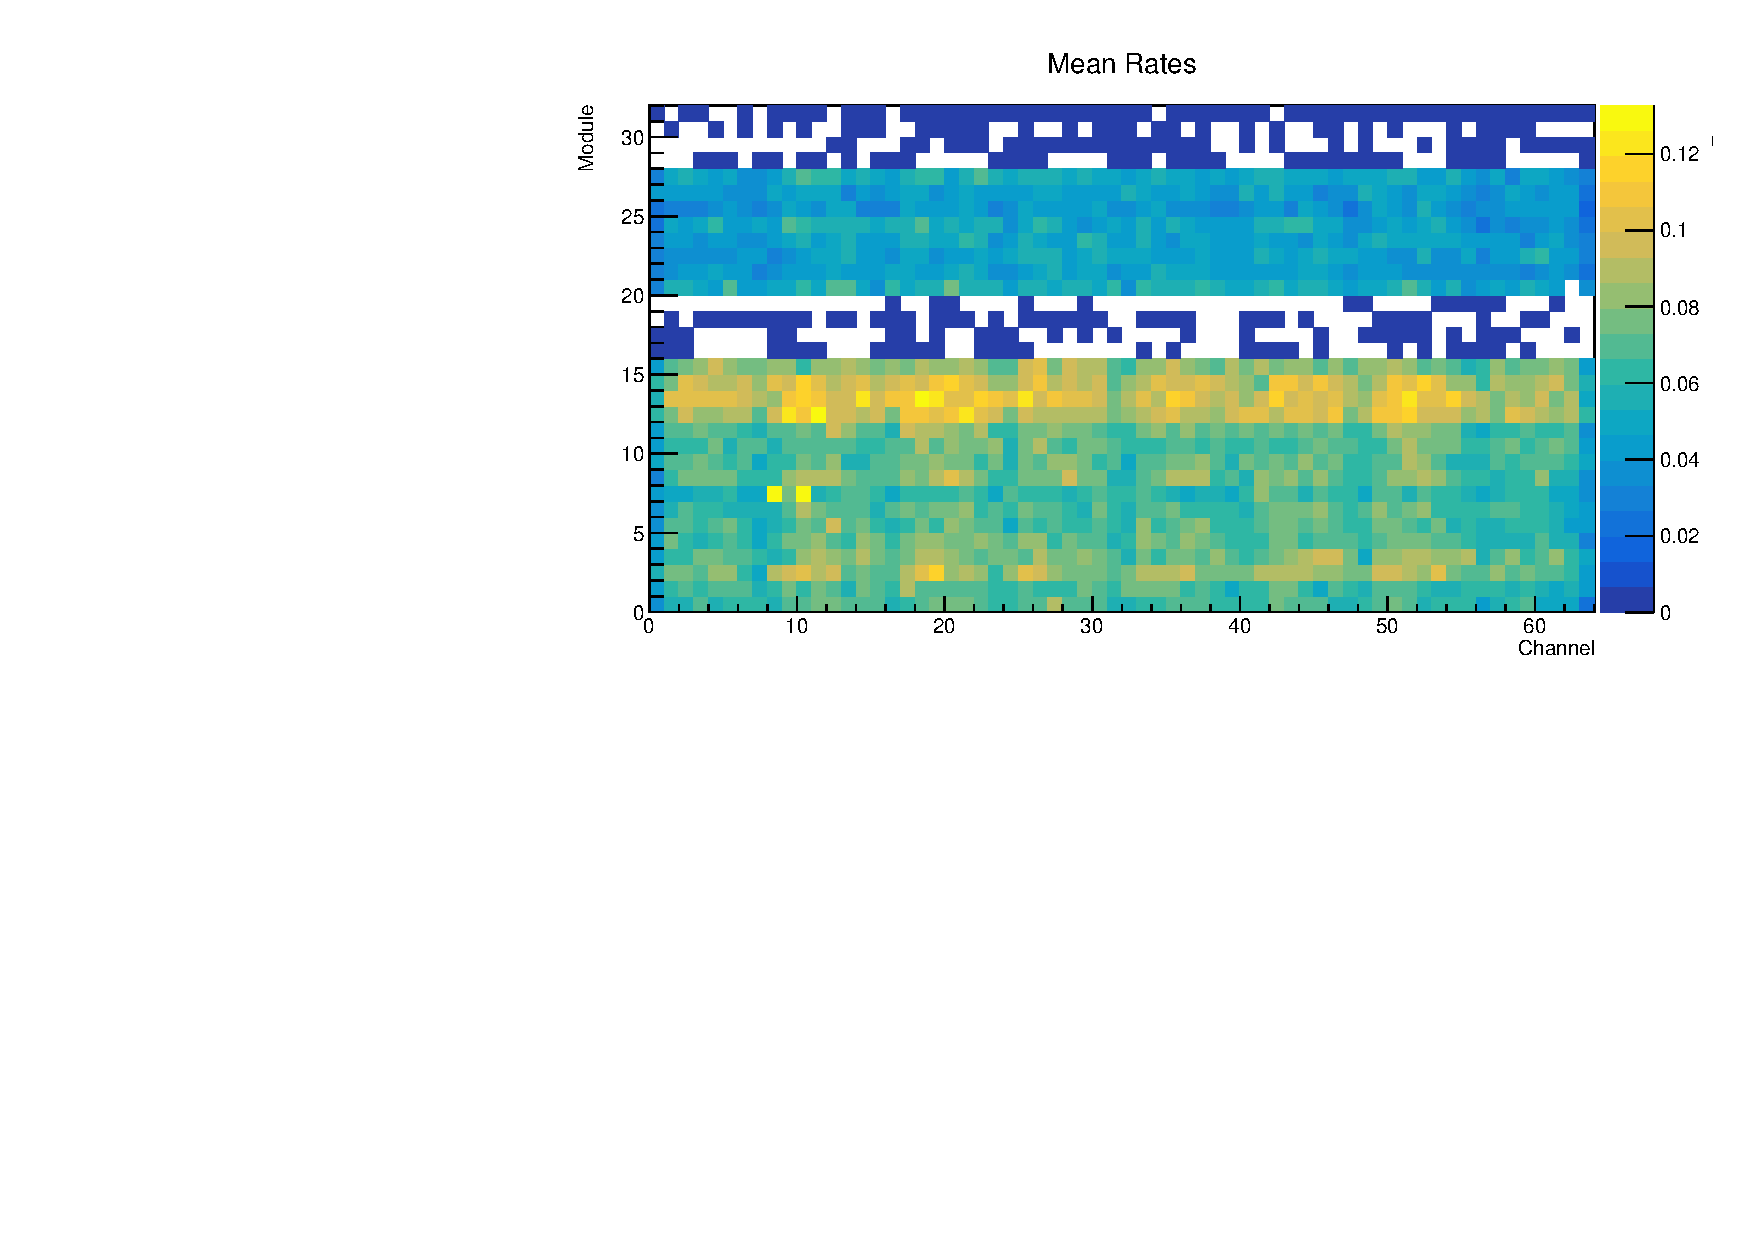
\includegraphics[width=\textwidth]{figures/crt_rate_om.pdf}
		\caption {Rate of hits measured by each CRT channel. The channels are
		arranged into a 2D histogram based on the module number and the channel
		number within each module.}
		\label{fig:crt_rate_om}
	\end{subfigure}

	\begin{subfigure}[b]{0.8\textwidth}
		\centering
		\vspace{3mm}
		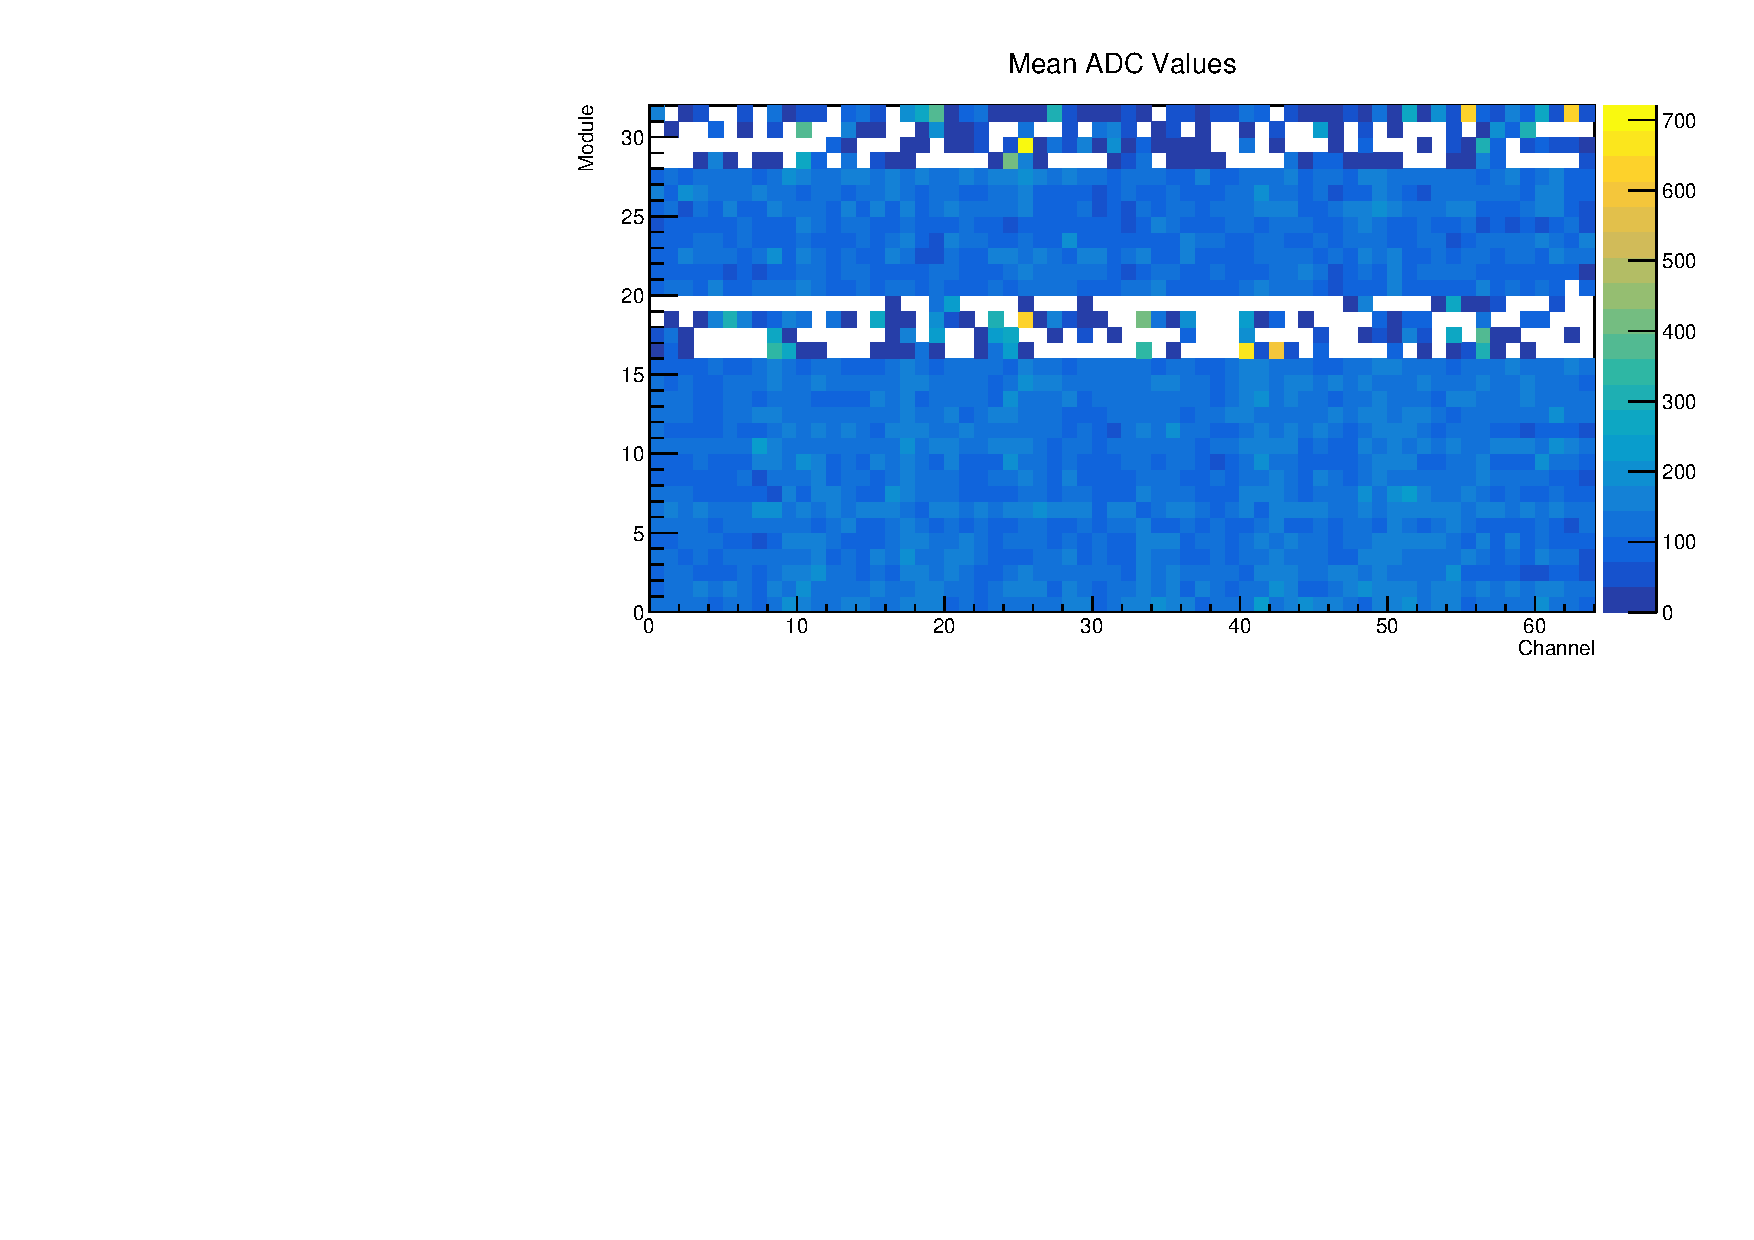
\includegraphics[width=\textwidth]{figures/crt_adc_om.pdf}
		\caption {Average ADC value of hits measured by each CRT channel. The 
		channels are arranged into a 2D histogram based on the module number and the 
		channel number within each module.}
		\label{fig:crt_adc_om}
	\end{subfigure}

	\caption
	[Examples of online monitoring plots for the cosmic--ray tagger.]
	{Examples of online monitoring plots for the cosmic--ray tagger.}
	\label{fig:crt_OM}

\end{figure}

\subsection{Monitoring Web Interface}
The plots from the data analysis are stored in a ROOT file on the \protodune{}
DAQ servers. This data is viewable from anywhere in CERN via a web interface
which was adapted for \protodune{} from LHCb's Monet\cite{Adinolfi_2017}. 
Monet consists of a Flask web application\cite{flask} which uses 
Bokeh\cite{bokeh} to render plots for display, ROOT\cite{ANTCHEVA20092499} and 
NumPy\cite{numpy} are used to process the monitoring data in preparation for 
display.

Two important modifications were made to Monet for \protodune{}: efficiency 
improvements, which were required to handle the large amounts of data in the 
event displays, and the addition of a separate rendering server with 
additional capabilities. 

The components of the web interface, and their connections, are outlined in 
Figure \ref{fig:monet_flow}. When a user makes a request, for example to open 
a new page of plots or a to interact with a plot, the request is sent to the 
display server which decides what to do with it. Depending on the nature of 
the request, the display server will then interact with the histogram database 
and/or the rendering server, before updating the plots and displaying them to 
the user. 

\begin{figure}

	\centering

	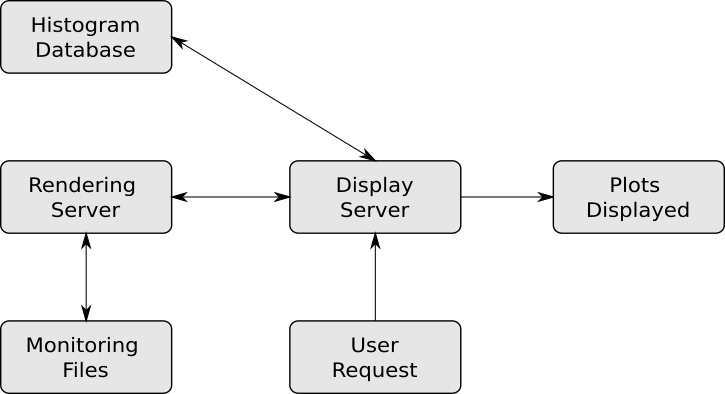
\includegraphics[width=0.7\textwidth]{figures/monet_flow.png}

	\caption
	[Data flow diagram for the web interface in the \protodune{} online 
	monitoring system.] 
	{Data flow diagram for the web interface in the \protodune{} online 
	monitoring system. The display server is responsible for handling user
	requests by communicating with the histogram database and rendering server,
	which collect plots from the monitoring files to display to the user.} 
	\label{fig:monet_flow}

\end{figure}

The plots in the monitoring files are organised into pages in Monet. Each page
can contain any number of plots which are organised into an array on the screen,
an example of this is shown in Figure \ref{fig:monet_page}. The histogram 
database is responsible for the details of each of these pages, this includes
the plots on each page, their locations, and the relevant rendering options for
each plot. When a new page is requested, the display server retrieves these
details from the histogram database before requesting the rendering server to 
render the plots.

\begin{figure}

	\centering

	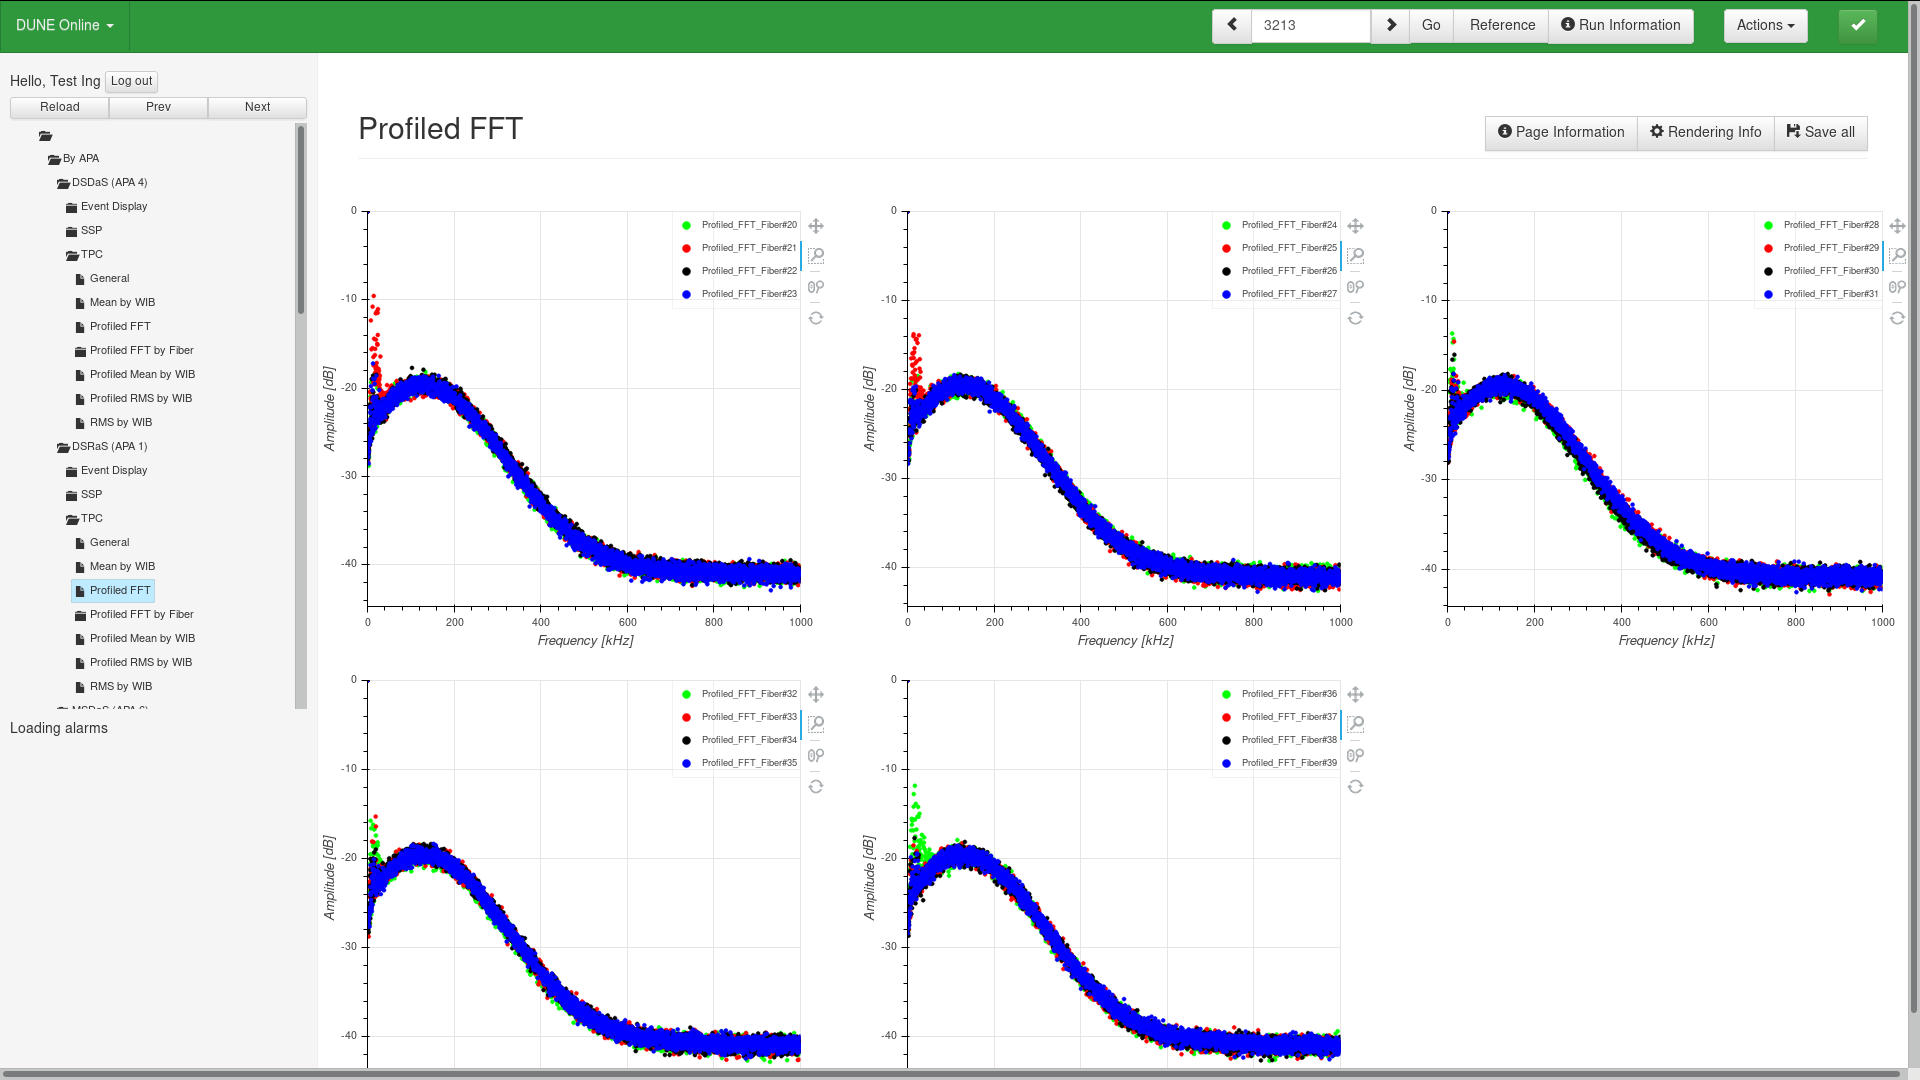
\includegraphics[width=\textwidth]{figures/profiled_fft_monet.png}

	\caption
	[An example of an online monitoring page.] 
	{ An example of an online monitoring page, containing the profiled FFTs for
	all FEMBs on APA 1. Users are able to select which page to display from the
	folder list on the left, select a run number in the top bar, and interact 
	with each plot, e.g. zooming in on a specific region.} 
	\label{fig:monet_page}

\end{figure}

The rendering server is responsible for visualising the plots from the 
monitoring ROOT files, it is capable of rendering all 1D and 2D ROOT plots. In 
LHCb's Monet rendering is handled directly on the display server, however in 
\protodune{} an additional rendering server was added. By separating the 
rendering processes onto their own server, additional functionality is 
possible. The main advantage of the rendering server is that it enables the 
OM to utilise a dynamic binning algorithm to scale the resolution of the 
displayed images in response to user interaction. This is mainly used for the 
event displays; the event display is initially loaded in low resolution, but 
if a user is interested in a specific region of the event display they can 
zoom in on the region of interest, which is then displayed at a higher 
resolution by the dynamic binning algorithm as demonstrated in Figure 
\ref{fig:dynamic_binning}.

\begin{figure}

	\centering

	\begin{subfigure}[b]{\textwidth}
		\centering
		\vspace{3mm}
		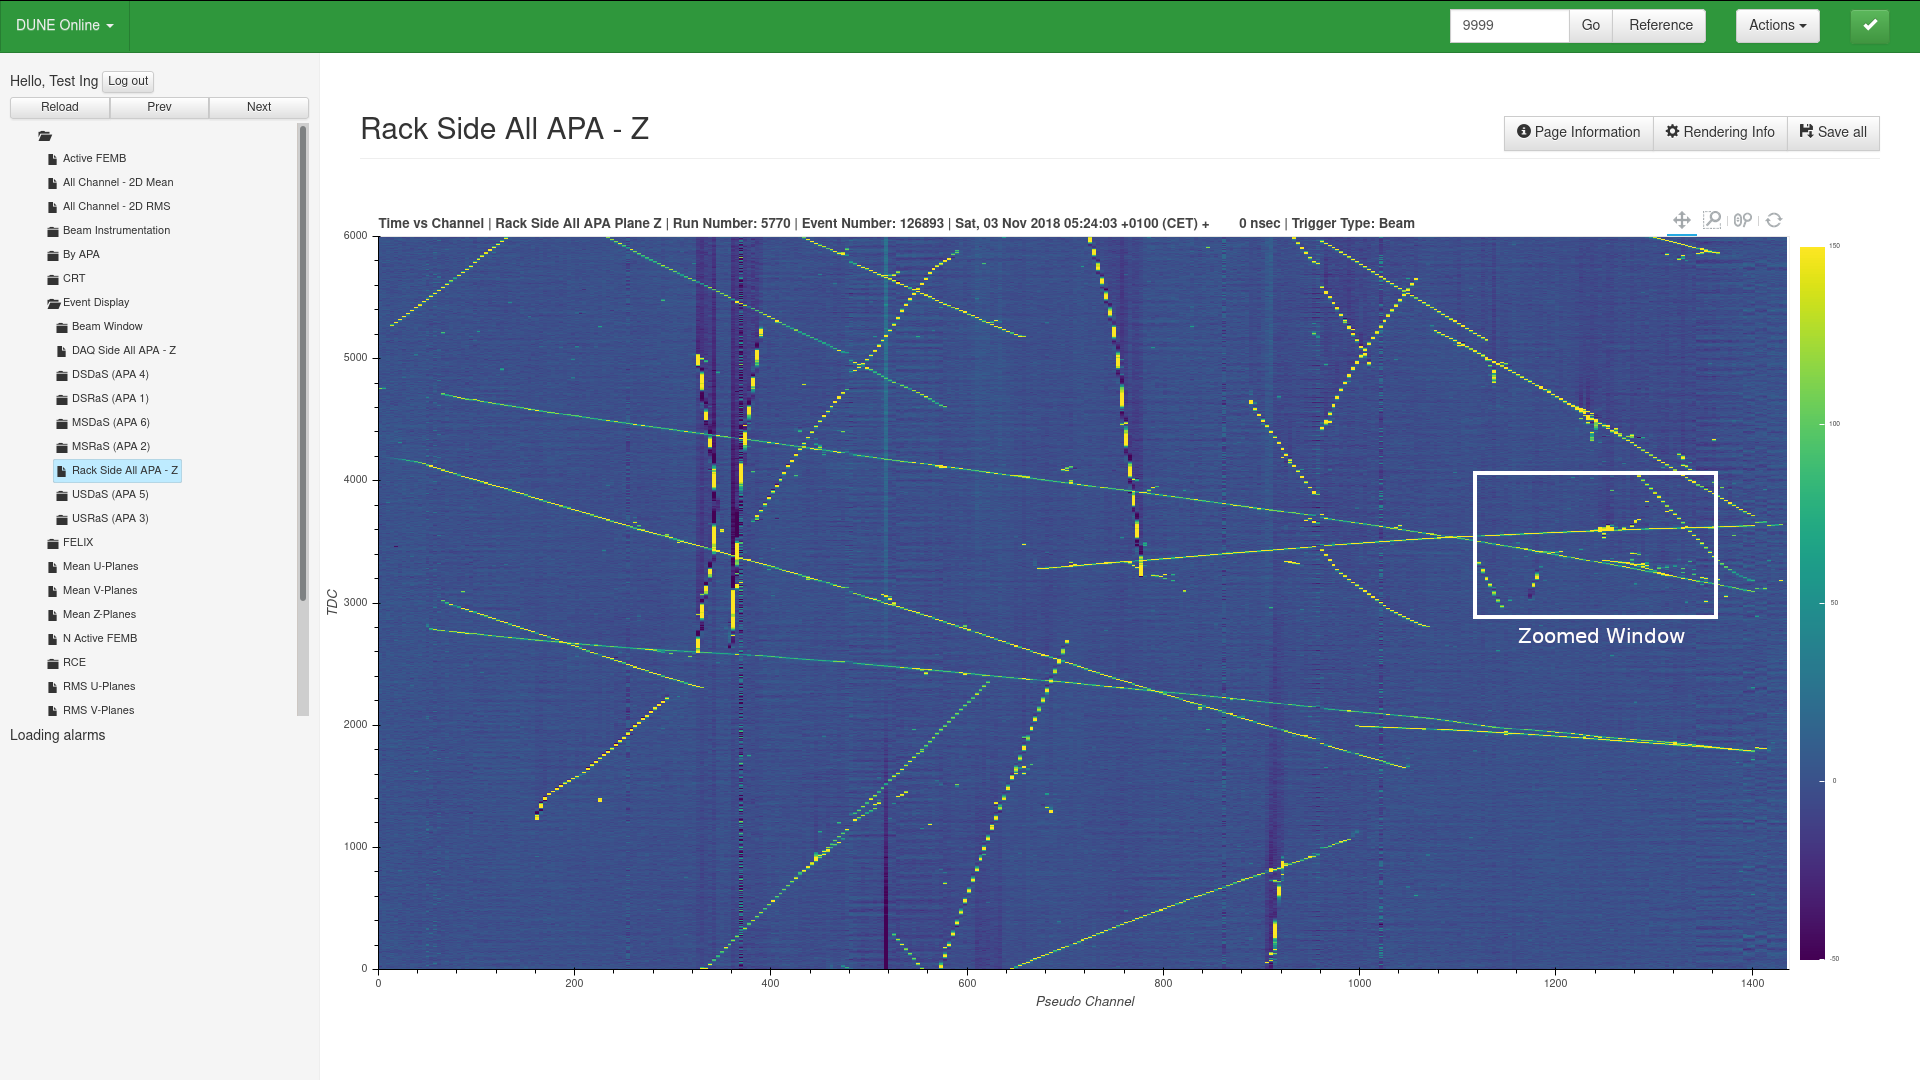
\includegraphics[width=\textwidth]{figures/zoomed_out.png}
		\caption {The downscaled version of the event display, showing the data from 
		all three APAs on one side of the TPC. The white square represents the 
		zoomed region in Figure \ref{fig:zoomed_in}.}
		\label{fig:zoomed_out}
	\end{subfigure}

	\begin{subfigure}[b]{\textwidth}
		\centering
		\vspace{3mm}
		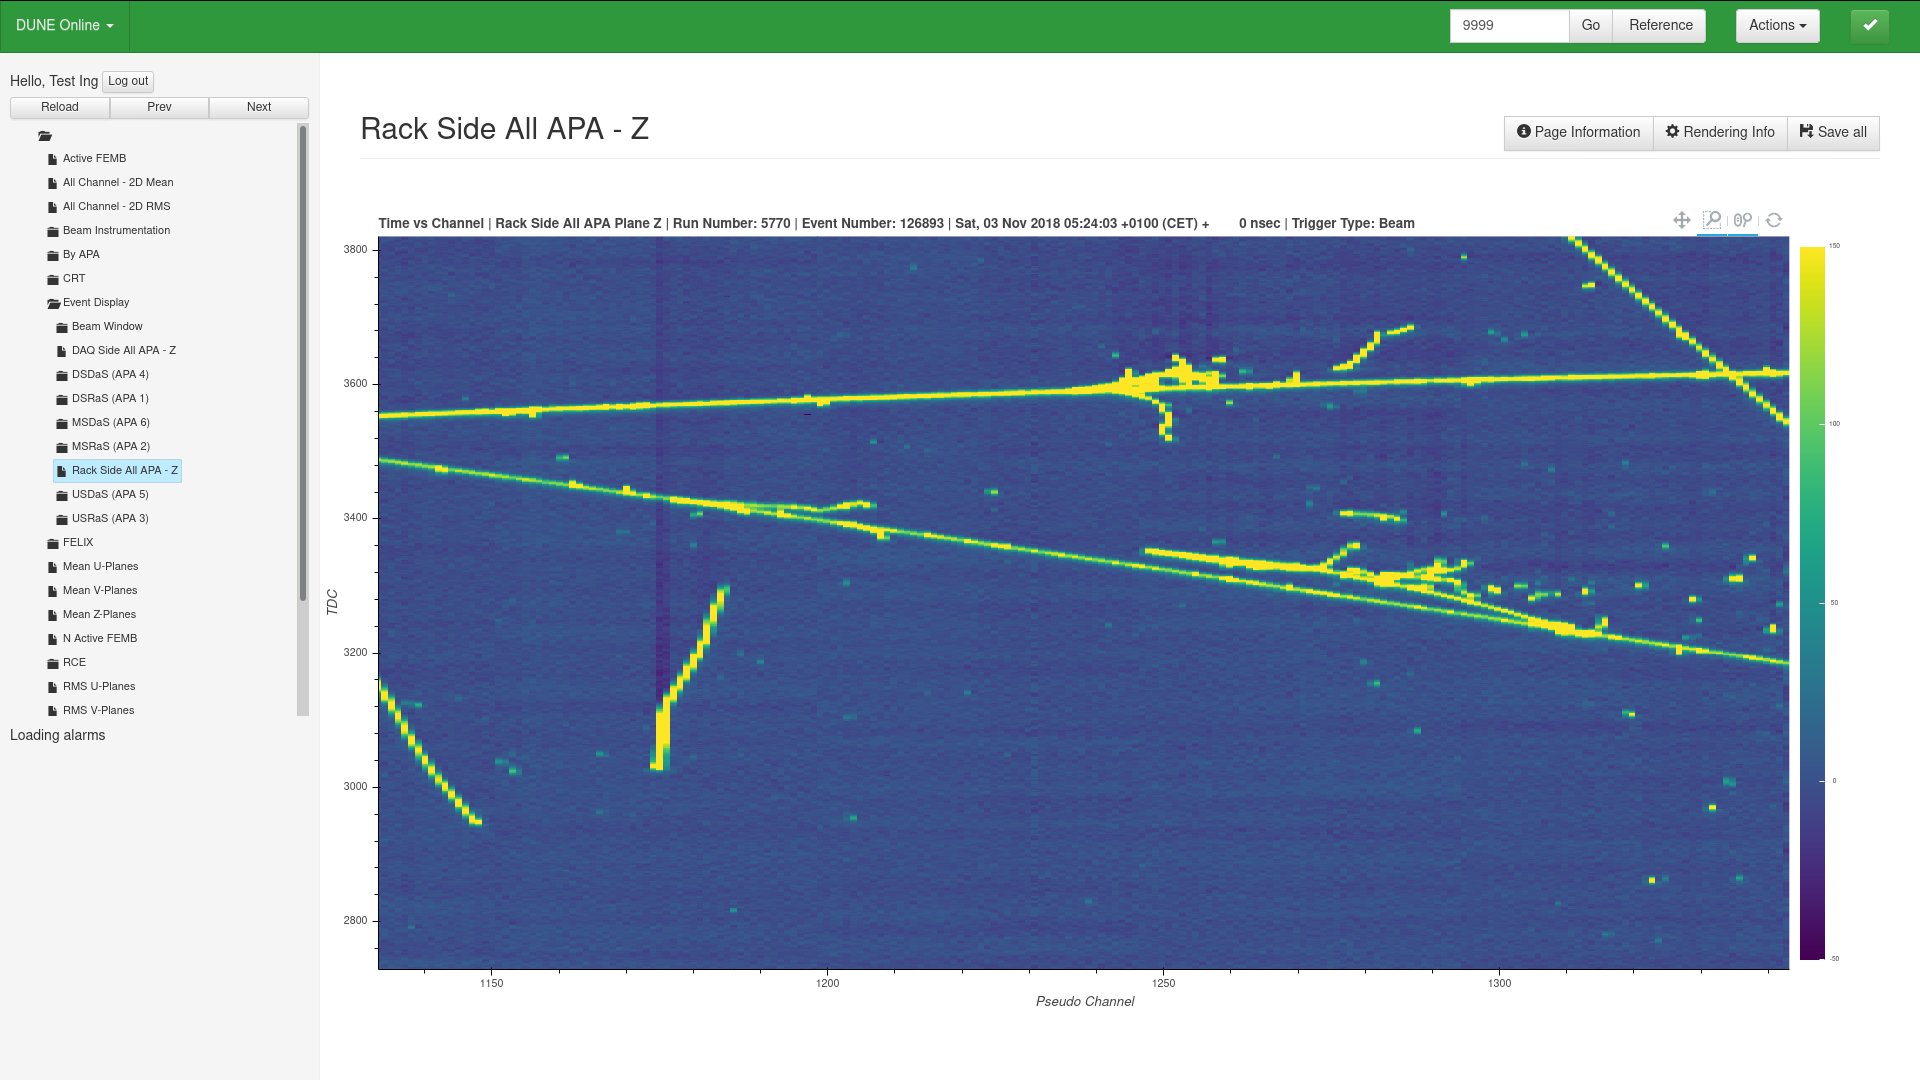
\includegraphics[width=\textwidth]{figures/zoomed_in.png}
		\caption {Zoomed region of the event display, which is shown at a higher
		resolution.}
		\label{fig:zoomed_in}
	\end{subfigure}

	\caption
	[Example of the dynamic binning algorithm in the \protodune{} online
	monitoring system.]
	{ Example of the dynamic binning algorithm in the \protodune{} online
	monitoring system. }
	\label{fig:dynamic_binning}

\end{figure}

The other significant modification to Monet was to modify the data handling to 
significantly improve the efficiency of data transfer to the renderer.
When Monet was first adapted for \protodune{} it was too slow to render some 
of the larger plots, such as event displays, which would initially take 
minutes to render. By improving the efficiency of the data transfer from ROOT 
to Bokeh, the rendering time was reduced to around 4 seconds per event display.

\subsection{System Performance and Possible Improvements}
In the \protodune{} technical design report\cite{Abi:2017aow}, the proposed 
online monitoring system was described as being able to \say{provide data 
quality assurance in real--time}. In practice, the response time is around one 
minute. During this time, 10 events will have been processed for each set of 
plots, however, the event displays and TPC FFTs only contain data from one 
event.

The performance of the OM was found to be satisfactory for the operation of the
\protodune{} detector during the beam runs in 2018. However, there is room for
improvement, particularly in terms of the turnaround between the data readout 
and plots being available in the OM. In the current system the latency is made 
up of four primary components:
\begin{itemize}
	\item Waiting for the input data file containing the events to be closed.
	\item Processing the data with the Analyser Modules.
	\item Writing the monitoring plots to disk.
	\item Merging TPC monitoring with plots from external systems.
\end{itemize}
The latency introduced by each of these components have an approximate ratio of 
40:15:30:15. 

Input file closure currently makes up the most significant portion 
of the latency. In the current system, the OM processes have to wait for the 
event builders to finish processing a batch of 100 events and close the output 
file before they can access the data. A shared memory system was proposed to 
tackle this problem, in this system the OM and event builders can 
simultaneously process the data as it leaves the detector. This would reduce 
the latency in the OM, by allowing it to analyse the data promptly as it is 
read out by the detector. Unfortunately, this system wasn't successfully 
implemented during the first beam run of \protodune{}, but it remains as a 
possible improvement to the monitoring system for any future \protodune{} 
runs, and for the DUNE Far Detector monitoring.

Additional improvements could be made to the latency, by using different 
computing hardware and improving the efficiency of the code. However, at the 
time of writing there are no specific improvements being investigated in these 
areas.

\subsubsection*{Authors Contributions to the \protodune{} Online Monitoring}
My main contributions to the online monitoring system in \protodune{} were made
from January 2018 to January 2019, these were: 
\begin{itemize}
	\item Writing code to produce plots for the Analyser Modules.
	\item Developing merger processes to merge the monitoring results from
		multiple DAQ servers, as well as external plots.
	\item Maintenance and development of the display server including:
	\begin{itemize}
		\item Significantly improving the efficiency of the plotting algorithms,
			such that event displays were possible in the OM.
		\item Integrating the rendering server into the display server.
		\item Integrating the histogram database into the display server.
	\end{itemize}
	\item Populating and maintaining the histogram database.
	\item Developing shell scripts for running the online monitoring jobs, and
		maintaining the online monitoring server.
	\item Ensuring the monitoring software remained up to date with changes to
		other DAQ software.
\end{itemize}
In addition, I worked as the on--call expert on the online monitoring system
during the \protodune{} beam run in 2018. I have remained involved in the OM 
since, mostly for small maintenance tasks. 

\chapter{\label{ch:energyloss}Electromagnetic Energy Loss in Liquid Argon} 

%%%%%%%%%%%%%%%%%%%%%%%%%%%%%%%%%%%%%%%%%%%%%%%%%%%%%%%%%%%%%%%%%%%%%%%%%%%%%%%%
% From COS
% This chapter will cover in more detail both the theory and measurement of
% electromagnetic energy loss in liquid argon. Energy loss for both electrons and
% photons will be discussed and the implications of this for electron
% reconstruction at different energy scales will be highlighted. 
% 
% The work in this section is complete and part of this work was reported in the
% document submitted for transfer of status.
%%%%%%%%%%%%%%%%%%%%%%%%%%%%%%%%%%%%%%%%%%%%%%%%%%%%%%%%%%%%%%%%%%%%%%%%%%%%%%%%

\minitoc

The energy loss of particles in liquid argon has important implications for the
reconstruction of different particles in a LArTPC, and will be relevant for the
reconstruction algorithms developed in Chapters \ref{ch:chargeid} and 
\ref{ch:michel} of  this thesis. This chapter will cover in more detail the 
theory of electromagnetic energy loss in liquid argon, highlighting the 
important features of the energy loss for muons, electrons, and photons.

\section{Electromagnetic Energy Loss in Matter}
In matter, charged particles lose energy through a number of small successive
collisions with the electrons in the material, and by radiative processes which
produce additional particles in the material. The relative importance of the
collision and radiative stopping power depends on the mass and the energy of the
particle. For most particles, which are heavy compared to the electron, 
radiative energy losses are not important until very high energies, e.g. for a 
muon they are not important until momenta of around 100 GeV. However, radiative 
energy loss become important for electrons at tens of MeV 
\cite{PhysRevD.98.030001}. As a result, different theories are used to 
describe the energy loss of heavy particles and electrons in matter.

\subsection{Energy Loss for Heavy Charged Particles}
For heavy particles such as muons at moderate energies, the mean rate of 
energy loss per unit distance is described by the Bethe equation,
\begin{equation}
	- \left< \frac{dE}{dx}\right> = K z^2 \frac{Z}{A} \frac{1}{\beta^2} 
	\left[ \frac{1}{2} \ln \frac{2 m_e c^2 \beta^2 \gamma^2 W_{max}}{I^2} -
	\beta^2 - \frac{\delta(\beta \gamma)}{2}\right].
	\label{eq:mu_stop}
\end{equation}
The constants in this equation are detailed in reference
\cite{PhysRevD.98.030001}. $Z$ and $A$ are the atomic number and mass number of
the medium, $z$ is the charge of the scattering particle, $W_{max}$ is the 
maximum energy transfer possible in a single collision, $I$ is the average 
ionisation energy, and $\delta$ is a density effect correction which is 
relevant in solids and liquids. 

Three important features of the energy loss in the Bethe formula are the minimum
ionising region, the relativistic rise, and the Bragg peak, these regions can be
seen in Figure \ref{fig:muon_dedx} which shows the $dE/dx$ for muons in argon 
as a function of momentum. 

\begin{figure}
	\centering
	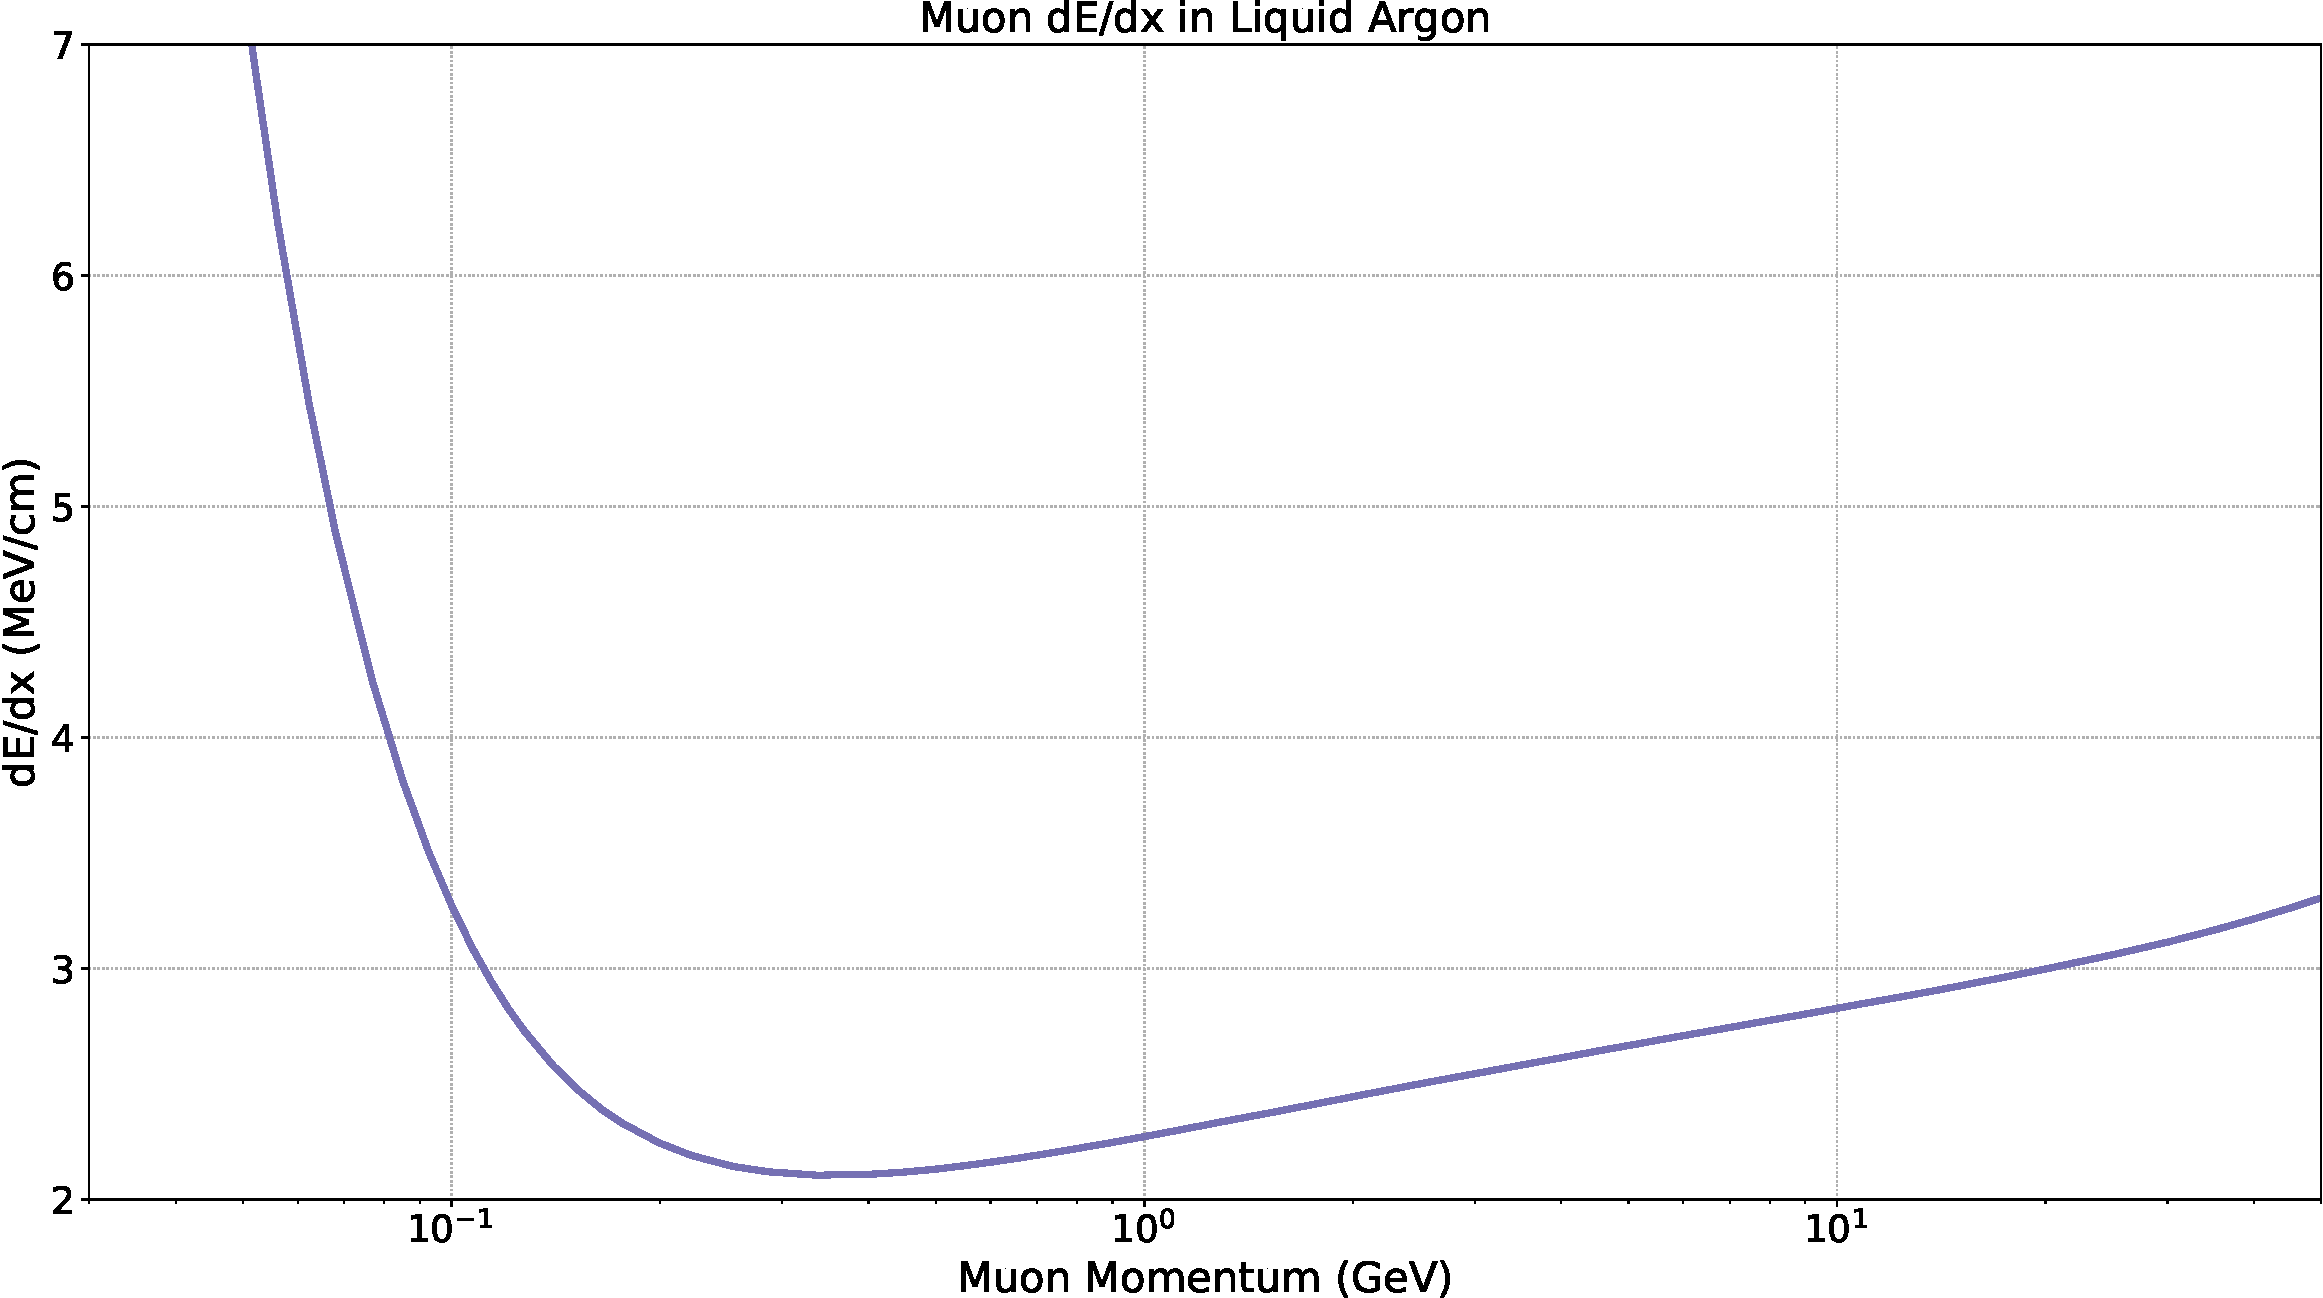
\includegraphics[width=\textwidth]{figures/muon_dedx_argon.pdf}
	\caption
	[Stopping power as a function of energy for muons in liquid argon.]
	{ Stopping power as a function of energy for muons in liquid argon. Data from
	\cite{pdg_atomictables}.}
	\label{fig:muon_dedx}
\end{figure}

\subsubsection*{Delta Rays}
Another feature of the electromagnetic energy loss of heavy particles that
impacts reconstruction in LArTPCs is delta rays. Delta rays are energetic
electrons, which are knocked out of their atoms when they collide with the heavy
particle. In liquid argon detectors these electrons are seen as small electron 
tracks which protrude from muon tracks. 

\subsection{Energy Loss for Electrons}
Electrons and positrons undergo different electromagnetic scattering processes
in matter, M{\o}ller scattering and Bhabha scattering respectively 
\cite{10.2307/96528, 10.2307/96479}. These processes, which dominate electron 
and positron energy loss at low energies, have different cross sections, which 
modify the energy loss in each case. At higher energies, radiative processes 
such as bremsstrahlung dominate. The two components of the electron stopping 
power are known as the collision stopping power and the radiative stopping 
power.

\subsubsection*{Collision Stopping Power}
The collision stopping power of electrons and positrons is calculated with a
similar method to the heavy particle stopping power, where individual collisions
are considered in succession. The main difference in the calculations is the
cross sections used in the calculations, for electrons the M{\o}ller scattering
cross section is used, and for positrons Bhabha scattering is considered. Due to
the electrons and positrons having the same mass as their targets, the maximum 
energy transfer in a single collision, $W_{max}$, is the total kinetic energy. 
However, this value is halved for the case of electrons, due to the convention 
of calculating the stopping power for the final state electron with higher 
kinetic energy.

The stopping power based on M{\o}ller scattering of electrons gives,
\begin{align*}
	- \left< \frac{dE}{dx} \right> = \frac{1}{2} K \frac{Z}{A} \frac{1}{\beta^2}
	\bigg[ &\ln \frac{m_e c^2 \beta^2 \gamma^2 \left\{ m_e c^2 (\gamma - 1) / 2
	\right\} }{I^2} + (1 - \beta^2) \\
	&- \frac{2\gamma - 1}{\gamma} + \frac{1}{8} 
	\left(\frac{\gamma - 1}{\gamma}\right)^2 - \delta \bigg],
\end{align*}
while Bhabha scattering, which governs the positron stopping power, gives,
\begin{align*}
	- \left< \frac{dE}{dx} \right> = \frac{1}{2} K \frac{Z}{A} \frac{1}{\beta^2}
	\bigg[ &\ln \frac{m_e c^2 \beta^2 \gamma^2 \left\{ m_e c^2 (\gamma - 1) 
	\right\} }{2 I^2} 
	+ 2 \ln 2  \\ &-\frac{\beta^2}{12} \left(23 + \frac{14}{\gamma + 1} +
	\frac{10}{(\gamma + 1)^2} + \frac{4}{(\gamma + 1)^3}\right) - \delta \bigg],
\end{align*}
where the terms have the same meanings as in Equation \ref{eq:mu_stop}
\cite{PhysRevD.98.030001}.

\subsubsection*{Radiative Stopping Power}
Above a few tens of MeV, electrons lose most of their energy through the 
emission of bremsstrahlung photons. Detailed discussion of the energy loss due
to bremsstrahlung emission is beyond the scope of this thesis, detailed
discussions are provided in \cite{PhysRevD.98.030001, Tsai:1973py}. Here, we 
discuss a simplified model, which highlights the important factors relevant for 
the work in this thesis.

At high energies, where the radiative energy loss is dominant, the energy loss
of electrons can be approximated as energy loss over a length scale, $X_0$,  
known as the radiation length.  In this approximation, the energy loss per 
unit distance due to bremsstrahlung is, 
\begin{equation*}
	- \left( \frac{dE}{dx} \right)_{brem} = \frac{E}{X_0}.
\end{equation*}
The radiation length, $X_0$, can be parametrised as,
\begin{equation}
	\begin{gathered}
		\frac{1}{X_0} = 4 \alpha r_e^2 \frac{N_A}{A} \left\{ Z^2 \left[L_{rad} - f(Z)\right] + Z
		L^\prime_{rad} \right\} \\
		\begin{aligned}
			f(Z) = \alpha^2 Z^2 \bigg[ &\frac{1}{1 + \alpha^2 Z^2} + 0.20206 - 0.0369
			\alpha^2 Z^2 \\ &+ 0.0083 \alpha^4 Z^4 -0.0002 \alpha^6 Z^6 \bigg],
		\end{aligned}
	\end{gathered}
	\label{eq:rad_length}
\end{equation}
where $L_{rad}$ and $L_{rad}^\prime$ are the so--called radiation logarithms,
which depend on the atomic number of the material\cite{Tsai:1973py}.

\subsubsection*{Critical Energy}
The critical energy is often defined as the energy at which the collision and 
radiative stopping power are equivalent, other definitions are also used, such
as the definition by Rossi, the energy where the ionisation loss per
radiation length is equal to the electron energy \cite{Rossi:1952kt}. Rossi's 
definition is equivalent to using the approximate $dE/dx$ calculated 
above\cite{PhysRevD.98.030001}. The value of the critical energy has important 
implications for reconstruction algorithms, because different approaches are 
often required above and below the critical energy. 

The critical energy is slightly different for electrons and positrons, in 
liquid argon they are both around 32 MeV, based on the Rossi definition 
\cite{pdg_atomictables}. This can be seen in Figure \ref{fig:electron_dedx}, 
which shows the total electron stopping power in liquid argon, in addition to 
the collision and radiative components which make up the total stopping 
power. 

\begin{figure}

	\centering

	\includegraphics[width=\textwidth]{figures/electron_dedx_argon.pdf}

	\caption
	[Stopping power as a function of energy for electrons in liquid argon.]
	{Stopping power as a function of energy for electrons in liquid argon. The
	contributions from collision and radiative stopping power are shown as dashed
	lines. The total stopping power is shown as a solid line. Data from 
	\cite{estar}.}

	\label{fig:electron_dedx}

\end{figure}

\subsection{Energy Loss for Photons}
A number of processes contribute to the energy loss of photons in matter, brief 
descriptions of the main processes are given below.

\subsubsection*{Photoelectric Effect}
The photoelectric effect occurs when a photon collides with an atom, X, the
photon is absorbed and electron is emitted from the atom. As a result, the atom 
is ionised. 
\begin{equation*}
	\gamma + X \rightarrow e^- + X^+
\end{equation*}

\subsubsection*{Compton Scattering}
Compton scattering occurs when a photon scatters incoherently from an electron
within an atom. The electron is typically liberated from the atom, and the
photon loses some of it's energy.
\begin{equation*}
	\gamma + e^- \rightarrow \gamma + e^-
\end{equation*}

\subsubsection*{Pair Production}
Pair production is the production of an electron positron pair, in the 
vicinity of an external electric field. During this process, the photon is
destroyed to produce the electron positron pair. In matter, the electric field
could be provided by either the electrons in the atom, or the nucleus of the
atom.
\begin{equation*}
	\gamma \rightarrow e^+ + e^-
\end{equation*}

\bigskip
\noindent
The cross section for these effects vary as a function of photon energy. The 
cross sections for each process in liquid argon, as well as the total photon 
cross section, are given in Figure \ref{fig:photon_xsec}. The Compton scattering
cross section is dominant from around 0.1 MeV to 10 MeV, after which the pair
production cross section dominates. 

\begin{figure}

	\centering

	\includegraphics[width=\textwidth]{figures/photon_xsec.pdf}

	\caption
	[Photon interaction cross sections in liquid argon.]
	{ Photon interaction cross sections in liquid argon. The contributions from
	Compton scattering, photo--electric effect, and pair production are shown as
	dashed lines. The total photon cross section is shown as a solid line. Data 
	from \cite{photon_xsec}.}

	\label{fig:photon_xsec}

\end{figure}

\subsubsection*{Photon Mean Free Path}
The mean free path of a photon is defined as the distance travelled by the
photon before it interacts with the material. The mean free path for photons
has two main components for photons in the MeV range, which are due to Compton
scattering and pair production. The mean free path is given by $\lambda = 1 / (n
\sigma)$, where $n$ is the number density of targets and $\sigma$ is the cross
section per target. The contribution to the mean free path from pair production
is related to the radiation length for electrons, $X_0$ from Equation
\ref{eq:rad_length}, by $\lambda_{PP} = (9/7) \; X_0$ \cite{PhysRevD.98.030001}.
The mean free path for photons in the MeV range is shown in Figure
\ref{fig:photon_mfp}, along with the main contributing cross sections. 

\begin{figure}

	\centering

	\includegraphics[width=\textwidth]{figures/photon_mfp.pdf}

	\caption
	[Photon mean free path in liquid argon.]
	{Photon mean free path in liquid argon. The mean free path based on the cross
	sections for Compton scattering, photo--electric effect, and pair production 
	are shown as dashed lines. The total photon mean free path is shown as a 
	solid line. Data from \cite{photon_xsec}.}

	\label{fig:photon_mfp}

\end{figure}

\subsection{Typical Interaction Signatures in \protodune{}}
As a result of the differences in energy loss, which depend on particle species
and energy, different particles leave distinct signatures in the detector.  
Figure \ref{fig:particle_signatures} shows the typical signatures of four 
types of interaction in a liquid argon TPC for events from \protodune{} 
data.

The most common interaction in \protodune{} is that of a cosmic--ray muon, seen
in Figure \ref{fig:muon_signature}. Muons, and other heavy particles, leave 
long tracks in the detector which deposit around 2.1 MeV/cm in the minimum 
ionising region. Alongside muon tracks, relatively high energy electrons, 
known as delta rays, are occasionally produced. Delta rays can be seen as 
electron activity along the length of the muon track.

Electrons in \protodune{} have two distinct signatures, which depend on the
energy of the electron. For high energy electrons, with energies above around
300 MeV, radiative energy loss dominates and showers are produced, an example 
of an electron shower can be seen in Figure \ref{fig:electron_signature}. 
These showers are the result of a cascade of electrons, which are produced by 
a chain of bremsstrahlung photons and electron positron pairs.

At energies in the tens of MeV range electrons have a different signature, 
which consists of a small electron track accompanied by a number of small 
ionisation energy deposits due to radiated photons. A common source of these
electrons in \protodune{} are Michel electrons, which are the electrons produced
when a muon decays at rest in the detector. An example of a typical Michel
electron event is shown in Figure \ref{fig:michel_signature}. The Michel 
electron is accompanied by the incoming Muon in the image, which is seen in the
image because the lifetime of the muon is shorter than the time it takes for 
the ionisation charge from the muon to drift away from the stationary muon.

As with electrons, photon interactions in liquid argon have two distinct
signatures at high and low energies. Low energy photons are typically produced
by the interactions of low energy electrons in the liquid argon, such as the
Michel electron interaction in Figure \ref{fig:michel_signature}. When these 
photons interact they produce small isolated energy deposits, which are 
created by the ionisation from either Compton scattered electron or an electron 
positron pair.

At high energies, photons produce similar interactions to high energy electrons,
which produce electromagnetic showers in the liquid argon. Their is a slight
difference in the $dE/dx$ in the first few cm of electron and photon showers, 
because the start of photon showers contain two electrons whereas the start of
electron showers only have one. This difference can can allow for electron and 
photon showers to be distinguished \cite{Acciarri:2016sli}. A common source of 
photon showers in \protodune{} are $\pi^0$ decays, shown in Figure 
\ref{fig:pi0_signature}, which produce a pair of photons.
\begin{figure}

	\centering
	% TODO: make these plots nicer

	\begin{subfigure}[b]{0.49\textwidth}
		\centering
		\includegraphics[width=\textwidth]{figures/muon_signature.png}
		\caption{Muon track with delta ray.}
		\label{fig:muon_signature}
	\end{subfigure}
	\hfill
	\begin{subfigure}[b]{0.49\textwidth}
		\centering
		\includegraphics[width=\textwidth]{figures/electron_signature.png}
		\caption{Electron shower.}
		\label{fig:electron_signature}
	\end{subfigure}

	\begin{subfigure}[b]{0.49\textwidth}
		\centering
		\includegraphics[width=\textwidth]{figures/michel_candidate.pdf}
		\caption{Michel electron.}
		\label{fig:michel_signature}
	\end{subfigure}
	\hfill
	\begin{subfigure}[b]{0.49\textwidth}
		\centering
		\includegraphics[width=\textwidth]{figures/pi0_signature.png}
		\caption{Photon showers from a $\pi^0$ decay.}
		\label{fig:pi0_signature}
	\end{subfigure}

	\caption
	[Typical particle interactions in \protodune{} for different particle species.]
	{Typical particle interactions in \protodune{} for different particle species.}

	\label{fig:particle_signatures}

\end{figure}

\chapter{\label{ch:ml}Neural Networks} 

\minitoc

\noindent
Machine learning (ML) is a field of research which studies algorithms that
can learn to make predictions from data, i.e. predict a set of output variables,
given a set of input variables. These algorithms typically take the form of a
multivariate function, which is used to predict the output\cite{Reed1999}.

ML algorithms are often classified into four groups based on two distinctions:
the expected output and the level of supervision. The first distinction is 
based on the nature of the output distribution expected from the network; 
regression algorithms are designed to predict the outputs of a continuous 
function, whereas classification algorithms aim to separate data into groups. 
The second distinction, between supervised and unsupervised algorithms, is 
based on the inputs used during training. In a supervised algorithm the true 
output is known, and the network's goal is to predict the true output, while 
in an unsupervised algorithm the true output is unknown, and the networks goal 
is to extract meaningful structure from the data\cite{Lecun2015}.

Chapters \ref{ch:chargeid} and \ref{ch:michel} of this thesis describe two 
examples of the application of Neural networks (NN) for event reconstruction 
in LArTPC data. These algorithms are classification algorithms based on the
supervised learning approach. This chapter will not attempt to provide a full 
survey of the available ML techniques, which are both numerous and diverse. 
Instead, this chapter will briefly describe the theory behind NNs, as well as 
providing details of the techniques used in the subsequent chapters. 

\section{Artificial Neural Networks}
Artificial neural networks (ANN) are a class of ML algorithm that draw their
inspiration from biological neurons. An ANN consists of a set of nodes, along
with connections between those nodes. The set of nodes and connections is 
often referred to as a graph or architecture. The nodes in the graph take the 
form of artificial neurons, which pass a number of inputs through an 
activation function to produce a single output, as depicted in Figure 
\ref{fig:neuron}. The output of each neuron is either distributed to 
subsequent neurons in the network, or it is part of the output of the network. 
\begin{figure}

	\centering

	\includegraphics[width = 0.7\textwidth]{figures/neuron.pdf}

	\caption
	[Graphical representation of an individual neuron in an artificial neural
	network.]
	{Graphical representation of an individual neuron (node) in an artificial 
	neural network.}

	\label{fig:neuron}

\end{figure}

One of the most widely used ANNs is the multi--layer perceptron 
(MLP)\cite{Reed1999}; this class of network consists of at least three layers 
of nodes: an input layer, one or more hidden layers, and an output layer. The 
layers are connected in a feedforward configuration, such that the graph of 
nodes contains no cycles. The layers of an MLP are often fully connected or 
dense, meaning that the output of every node is connected to the input of 
every node in the next layer of the network. An example of a fully connected 
MLP, with two hidden layers, is shown in Figure \ref{fig:mlp}. 
\begin{figure}

	\centering

	\includegraphics[width = 0.8\textwidth]{figures/mlp.pdf}

	\caption
	[A graphical representation of a multi--layer perceptron.]
	{ A graphical representation of a multi--layer perceptron. }

	\label{fig:mlp}

\end{figure}

Each node receives input from nodes in the previous layer, and uses the inputs
to calculate a response function. For the $i^{th}$ node in the $j^{th}$ layer 
of a network, 
\begin{equation*}
	a^{i,j} = \mathbf{w}^{i,j} \cdot \mathbf{x}^{j-1} + b^{i,j}
\end{equation*}
where $a^{i,j}$ is the response function, $\mathbf{w}^{i,j}$ is the weights
vector, $b^{i,j}$ is the bias, and $\mathbf{x}^{j-1}$ is the input vector from 
the previous layer. This response function is usually passed through a
nonlinear activation function, $f$, to produce the output from the node,
$y$, which is part of the input for the next layer,
\begin{equation*}
	\left(\mathbf{x}^j\right)_i = y^{i,j} = f \left( a^{i,j} \right).
\end{equation*}

\noindent
Some common choices for the activation function are the sigmoid function, the
hyperbolic tangent, the rectified linear unit (ReLU), and the softmax 
function\cite{Lecun2015, He2015, Szegedy2015}.
\begin{align*}
	\tag{Sigmoid} f(x) &= \frac{1}{1+e^x} \\
	\tag{Tanh}    f(x) &= \frac{e^x - e^{-x}}{e^x+e^{-x}} \\
	\tag{ReLU}    f(x) &= \mbox{max}\left( 0, x \right) \\
	\tag{Softmax} f(x_i) &= \frac{e^{x_i}}{\displaystyle\sum_j e^{x_j}}
\end{align*}
In the softmax function, the index $i$ indicates the current node, and the index
$j$ includes all nodes in the current layer. This construction ensures that 
the outputs from a softmax layer sum to one, and as such this unit is commonly 
used in categorisation tasks when the output must belong to one of a given set 
of categories. The benefits and drawbacks of these common activation functions 
will be discussed later in this chapter, when the modification of weights 
with the backpropagation algorithm will be discussed.

The weights and biases of the nodes in an MLP can be adjusted to make accurate 
predictions of data. For a classification task, there are typically as many
output nodes as there are classes, with output values in the range zero to one. 
The output value of a classification network quantifies how well the input
represents each class, based on the networks prediction. In principle, MLPs 
are able to approximate any function to arbitrary precision with a 
single hidden layer\cite{Cybenko1989ApproximationBS}; however, there is no 
limit on the number of nodes required in order to achieve a good 
approximation. In practice, networks with additional hidden layers can attain 
the required precision with fewer nodes than a network with a single hidden 
layer, however, there are diminishing returns with more than a few hidden 
layers\cite{Reed1999, Lecun2015}.

\subsection{Convolutional Neural Networks}
The convolutional neural network (CNN)\cite{Jackel2008, Szegedy2015, 5537907}, 
is an extension of the MLP, which has had considerable success particularly in 
image classification tasks. These architectures address some of the drawbacks 
of the traditional MLP, particularly when evaluating data with a high 
dimensional input. When working with high dimensional inputs, networks with a 
fully connected network architecture tend to have a large number of neurons 
and high computational cost. In addition, for spatially correlated data, such 
an architecture does not take into account the local spatial structure of the 
data, instead focussing on all the data at once. A CNN attempts to resolve 
these issues by exploiting the local spatial structure of the data.

In a CNN the singular input neurons of a traditional MLP are replaced by
convolutional kernels. A convolutional kernel is a matrix containing a set of 
weights, which are multiplied pixel--by--pixel with small regions of the input 
image. The convolution operator is defined as, 
\begin{equation*}
	\left( x * y \right)_i = \sum_{j = - \infty}^{\infty} x_j \; y_{i-j},
\end{equation*}
where $x$ and $y$ are discrete sequences. In the machine learning context, $y$
represents the image, and $x$ the convolutional kernel, which are both finite in
extent. Therefore, they are defined to be zero outside of their boundaries, and
the sum range can be reduced to $\left[0, N\right]$, where $N$ is the number 
of pixels in the kernel. The convolution operation is applied to all pixels in 
the input image, which are then replaced by the resulting convolution in the 
next layer of the network. Many convolutional kernels are used in each layer 
of the network, each producing an output image which is passed to the next 
layer. 

Convolutional kernels are sometimes referred to as feature detectors, which 
emphasises the fact that each kernel identifies a given feature in the data, 
based on the weights in the kernel matrix. The output image from each kernel 
is known as a feature map, reflecting the fact that they represent the spatial 
distribution of the features learned by a given feature detector. A common type
of feature detector is the edge detector, such as the Sobel edge 
detector\cite{kanopoulos1988design}. Figure \ref{fig:edge_detector} shows an
example of the feature map produced when a Sobel edge detector is applied to an
image.
\begin{figure}

	\centering

	\begin{subfigure}[b]{0.49\textwidth}
		\centering
		\includegraphics[width=\textwidth]{figures/ed_input.jpg}
		\caption{Input Image.}
		\label{fig:ed_input}
	\end{subfigure}
	\hfill
	\begin{subfigure}[b]{0.49\textwidth}
		\centering
		\includegraphics[width=\textwidth]{figures/ed_feature_map.jpg}
		\caption{Feature Map.}
		\label{fig:ed_feature_map}
	\end{subfigure}

	\caption
	[Application of a Sobel edge detector to an image.]
	{Application of a Sobel edge detector to an image. Images from
	\cite{edge_detector}.}

	\label{fig:edge_detector}

\end{figure}

\subsubsection*{Pooling}
The use of images as network input often drastically increases the number of
input parameters for a network. When combined with a large number of
convolutional filters this can lead to a dramatic increase in the computational
cost of training a network. Pooling\cite{5537907} is a downsampling technique 
designed to reduce the number of parameters in the network and, therefore, 
reduce the computational cost of making predictions. In pooling algorithms
the data from each $m \times n$ region of the input is downsampled to a single 
value, the downsampled image is used as the input for the next layer of the 
network. Two common pooling algorithms are max pooling and average pooling; in 
max pooling the maximum value from within the downsampling region is used, 
whereas average pooling uses the average value from the region.

\bigskip\noindent
While convolutions are able to extract features from the data, they typically
are not able to make predictions in the desired format for classification tasks.
Therefore, after convolutions, data is typically flattened and passed through
one or more dense layers in order to produce the classification prediction. A
graphical representation of a typical CNN architecture is shown in Figure
\ref{fig:cnn_layer}, it includes convolutional, pooling, and dense layers.
\begin{figure}
	\centering
	\includegraphics[width = \textwidth]{figures/cnn_layer.png}
	\caption
	[A graphical representation of a convolutional neural network.]
	{ A graphical representation of a convolutional neural network. Figure
	generated with \cite{cnn_diagrams}.}
	\label{fig:cnn_layer}
\end{figure}

\subsection{Residual Neural Networks}
Adding more layers to a neural network usually improves the performance,
typically with each subsequent layer, the network is able to learn more complex 
features of the image with which to make it's classification. In fact, adding 
more layers should never decrease the performance of a network, as the new 
layers could be set to the identity, which would result in the same output 
from the network. However, it has been demonstrated that adding too many 
layers to a simple neural network will reduce performance, suggesting that the 
optimisation of larger networks leads to some form of 
degradation\cite{He_2016_CVPR}.

One method which has been shown to counter the degradation of deep networks, 
is the use of residual neural networks (ResNet). In a ResNet, the input to 
each layer is combined with the results of the convolutions as part of the 
input to a future layer; in effect, the identity transformation has been added
to the set of operations in the layer. This results in the weights of each layer
remaining as small perturbations around the identity, rather than large
corrections which would be required to build up the output from zero. This is a 
common qualitative intuition for why this method improves optimisation of the 
network weights. An example of these shortcut connections is shown in Figure 
\ref{fig:short_connect}\cite{He_2016_CVPR}. 
\begin{figure}
	\centering
	\includegraphics[width = 0.6\textwidth]{figures/short_connect.pdf}
	\caption
	[An example of a shortcut connection in a convolutional neural network.]
	{An example of a shortcut connection in a convolutional neural network.
	Figure from \cite{He_2016_CVPR}.}
	\label{fig:short_connect}
\end{figure}

\section{Supervised Learning}
Supervised learning is the process of teaching a neural network to accurately
predict the correct output, or ground truth, for a given input. The network is 
optimised by minimising the loss function, which quantifies the difference 
between the network output and the ground truth. The choice of loss function 
is dependent on the problem being considered and, therefore, specific examples 
will be discussed in subsequent chapters, which will detail the CNN algorithms 
developed as part of this thesis.

The output of a neural network, $g(x)$, is the result of a chain of function 
evaluations and matrix multiplication; for a network with $n$ layers,
\begin{equation*}
	g(x) = f^n(W^n f^{n-1}(W^{n-1} \;...\; f^1(W^1 x) \;...\; ).
\end{equation*}
where $g$ is the output of the network, $x$ is the input, $f$ are the 
activation functions for each layer, and $W$ are the weights for each layer. 
The loss of the network is given by the loss function, $L$, evaluated on the 
output of the network and the ground truth, $y$,
\begin{equation*}
	L(y, g(x)).
\end{equation*}

\noindent
To make accurate predictions with a NN, quantified by the loss function, the
weights and biases of the network need to be optimised. The backpropagation
algorithm\cite{Rumelhart1986} is currently the most widely used algorithm for
minimising the loss function by adjusting the weights and biases in the network.

\subsection{The Backpropagation Algorithm}

Consider the weight for the $j^{th}$ node in the $l^{th}$ layer of a network for
an incoming connection from the $i^{th}$ node from the previous layer, 
$W^l_{ij}$. The loss function varies with respect to these weights as 
$\partial L/\partial W^l_{ ij }$. If the weights are modified with, 
\begin{equation} 
	\Delta W^l_{ ij } = -\eta \frac{\partial L}{\partial W^l_{ ij }},
	\label{eq:delta_w}
\end{equation}
for positive learning rates, $\eta > 0$, the loss will be reduced provided it
is not already too close to the minimum. The backpropagation algorithm provides 
a means for calculating the derivatives required to adjust the weights in each 
layer.

Applying the chain rule to the right hand side of Equation \ref{eq:delta_w},
\begin{equation}
	\frac{\partial L}{\partial W^l_{ij}} = \frac{\partial L}{\partial a^l_j} \;
	\frac{\partial a^l_j}{\partial W^l_{ij}},
	\label{eq:backprop_chain_rule}
\end{equation}
where $a^l$ are response functions for the nodes in layer $l$. The derivative 
of the response function with respect to the weights, is simply the input from 
the previous layer,
\begin{equation}
	\frac{\partial a^l_j}{\partial W^l_{ij}} = \frac{\partial}{\partial W^l_{ij}}
	\left( \sum_{k = 1}^{n_l} W^l_{kj} x^{l-1}_{k} \right) = x^{l-1}_i,
	\label{eq:backprop_d_activ}
\end{equation}
where $x^{l-1}$ are the outputs from layer $l-1$, and $n_l$ is the number of 
nodes in layer $l$. The other term, which is often denoted as $\delta^l_j$, is 
known as the error; this term will be discussed shortly. Combining Equations 
\ref{eq:backprop_chain_rule} and \ref{eq:backprop_d_activ} gives,
\begin{equation*}
	\frac{\partial L}{\partial W^l_{ij}} = \delta^l_j \; x^{l-1}_i.
\end{equation*}

\noindent
The value of the error depends on the loss function being used in each 
particular model. The error can also be shown to have a recursive relationship 
via the chain rule,
\begin{align*}
		\delta^l_j = \frac{\partial L}{\partial a^l_j} &= \sum_{k=1}^{n^{l+1}} 
		\frac{\partial L}{\partial a^{l+1}_{k}}\frac{\partial a^{l+1}_k}{\partial 
		a^l_j}\\ 
		&= \sum^{n^{l+1}}_{k = 1} \delta^{l+1}_k \frac{\partial a^{l+1}_k}{\partial 
		a^l_j},
\end{align*}
where the sum is over all nodes in layer $l+1$. Using the definition of the 
response function to simplify this further,
\begin{align*}
		\frac{\partial a^{l+1}_k}{\partial a^l_j} &= \frac{\partial}{\partial a^l_j} 
		\left( \sum^{n^l}_{p=1} W^{l+1}_{pk} f(a^l_p) \right) \\ 
		&= W^{l+1}_{jk} \; f^\prime(a^l_j)
\end{align*}
where $f$ is the activation function. The error is, therefore,
\begin{equation*}
	\delta^l_j = \sum^{n^{l+1}}_{k=1} \delta^{l+1}_k W^{l+1}_{jk} f^\prime(a^l_j),
\end{equation*}
which depends on the value of the error in the following layer.

Based on these manipulations with the chain rule, the backpropagation 
algorithm works as follows,
\begin{enumerate}
	\item Calculate the forward pass, while storing the results for $g(x)$, 
		$a^l_j$, and $x^l_j$.
	\item Starting at the output layer, calculate the derivatives, going backwards
		through the network. 
	\begin{itemize}
		\item Store the results for $\delta^l_j$ from each layer, to use when 
			calculating subsequent layers.
	\end{itemize}
	\item Update the weights according to the update rule in Equation 
		\ref{eq:delta_w}.
\end{enumerate}

\noindent
The backpropagation algorithm is used to calculate the gradients in order to
adjust weights in a neural network. There are a number of optimisation 
algorithms for adjusting the weights, such as mini--batch stochastic gradient 
descent (SGD)\cite{10.1145/2623330.2623612} and adaptive momentum estimation 
(Adam)\cite{KingmaD.P.2015AAMf}. The details of these algorithms are not 
important for the discussion in this thesis and, therefore, they will only be 
mentioned in passing here. A review of gradient descent optimisation 
algorithms can be found in \cite{ruder2016overview}. Some methodologies are 
common among many optimisation techniques, three important examples are the 
ideas of mini--batches, training iterations, and training epochs. A 
mini--batch is a small sample of the input data, on which the backpropagation 
algorithm is applied simultaneously, this corresponds to one training 
iteration. A training epoch consists of a number of training iterations, and 
corresponds to one cycle through the full training dataset, such that the 
network has been trained on every training example exactly once.

\subsubsection{The Choice of Activation Function}
The rate of learning in the backpropagation algorithm is dependent on the
derivative of the activation function, therefore, the choice of activation
function has an impact on learning. There are two important factors when
considering the impact of this choice on the rate of learning, these are the 
computational cost of calculating the derivative, and the gradient of the 
function. 

Traditional activation functions, such as sigmoid and tanh, are usually 
bounded and differentiable, however the presence of exponentials makes 
computing the gradients expensive. They also typically have vanishing 
gradients in the tails, which can lead to slow learning if the value of the 
activation is consistently in the tail of the distribution. 

The ReLU activation function is much cheaper to compute, and while the 
gradient is undefined at zero, in practice this is not a problem. One issue 
with ReLU units, is the vanishing gradient in the negative region. This can be 
resolved by implementing a small negative gradient below zero, which is known 
as a leaky ReLU or parametric ReLU\cite{He2015}. In practice, ReLU units have 
been found to outperform traditional sigmoid 
units\cite{Maas13rectifiernonlinearities, 10.5555/3104322.3104425}.

\subsection{Regularisation}
Regularisation refers to a set of techniques, which are used to prevent
over--fitting during the training of a NN. Over--fitting is the tendency
of models with a high number of parameters to produce overly complex models,
which fit the training data well but do not generalise to new data.
Regularisation ensures that the trained network can generalise well beyond the 
training data. A number of regularisation techniques can be used, such as 
applying penalty terms to the loss function, which are proportional to the 
square of the weights, ensuring that the weights stay relatively small. In 
this thesis two regularisation techniques are used: 
dropout\cite{Srivastava2014DropoutAS} and early 
stopping\cite{OrrGenevieveB.1998NNTo}.

The dropout algorithm sets a random subset of weights in each layer to zero for
each training iteration. Each weight has a probability, $p$, of being set to 
zero for each iteration. The product of the remaining weights is scaled up by 
a factor of $1/p$, which ensures that the size of the input to the activation 
function remains reasonably consistent. This reduced network is then trained 
using the backpropagation algorithm, and the non--zero weights are updated. 
During the next iteration, the set of non--zero weights is reselected, and a 
new reduced network is trained. Finally, after training, the final weights of 
the network are multiplied by $p$ to give the so--called model average of the 
reduced networks. The dropout algorithm with $p=0.5$, has proven to provide 
robust regularisation, and is a popular technique in the field\cite{Lecun2015}.

\say{Early stopping (is a) beautiful free lunch}, according to Geoff
Hinton\cite{Hinton2015}. It refers to the act of monitoring the loss on the 
validation set during training, in order to stop training before over--fitting 
has occurred. This technique can be applied alongside other regularisation 
techniques, and is used throughout this thesis, where the early stopping 
technique proposed by Lutz Prechelt\cite{OrrGenevieveB.1998NNTo} has been used.
This technique involves stopping training after the first checkpoint when the 
validation loss increases, and using the weights from the previous checkpoint. 

\chapter{\label{ch:chargeid}Hit Classification with Convolutional Neural Networks} 

\minitoc

The correct categorisation of particle interactions in the detector is a major
problem faced by any particle physics experiment. This typically starts with
identifying low level features of the interactions, which can then be used to
gradually build up a picture of the full interaction. In DUNE, the
classification of neutrino interactions requires identifying the lepton content
of the final state, and in \protodune{}, cross section analyses rely on
accurately identifying the particles in the interaction. Therefore, it is
important to be able to distinguish muons and pions from electrons in LArTPCs, 
or more generally, tracks from showers.

In order to build up a complete picture of an event, it is useful to begin by
identifying the small features of the interaction, which can then be used to
gradually build an understanding of the full event. In \protodune{}, the
smallest reconstructed features are the hits, which correspond to small charge 
depositions collected on individual wires. Classifying these hits provides
useful information for future analyses, and can potentially be used to aid
decision making during event reconstruction.

This chapter will describe an approach to hit classification in \protodune{} 
using machine learning techniques. Section \ref{hit-id} will detail an 
approach to hit classification in LArTPCs based on identifying the source of 
energy depositions with a convolutional neural network.  The performance of 
this approach will be analysed with ProtoDUNE--SP simulation and data in 
sections \ref{cnn-perf-sim} and \ref{cnn-perf-data} respectively. Finally,
Section \ref{cnn-appl} will briefly mention some of the current applications of
the network in \protodune{} analyses.

\section{Hit Classification with Convolutional Neural Networks} \label{hit-id}

Effective track shower separation forms the basis of many reconstruction
challenges in DUNE and \protodune{}; it is used to define pure calibration
samples, such as minimum ionising muons and $\pi^0$ decays, and it is an
important part of neutrino event reconstruction. Each event sample leaves a
unique signature in the detector, but the first step in reconstructing these
samples is the same, reconstructing tracks and showers, which can be combined to
build the final state. 

In a LArTPC, tracks and showers are built from collections of hits, these hits
have to be clustered and identified as track or shower objects. In this section,
we will describe a method for identifying the source of hits in the \protodune{}
LArTPC. The classification of each hit is stored as part of the reconstructed
output in LArSoft, and can be used by subsequent reconstruction and analysis
algorithms.

In addition to track and shower objects, Michel electrons are a useful 
calibration sample in LArTPCs. Michel electrons are electrons produced when a 
muon decays at rest, which have an energy spectrum in the range of 0--50 MeV. 
As discussed in Chapter \ref{ch:energyloss}, the critical energy for electrons 
in liquid argon is at around 30 MeV, at this point the collection energy
deposition and the radiative energy deposition are equal. Therefore, Michel 
electrons have a unique signature in LArTPCs, and they were included as a 
unique category in the classification algorithm.

\subsection{Data Preparation}

A CNN was designed to classify hits by using images of the detector readout
around the reconstructed hits. The network was trained to predict,
\begin{equation*}
	\left[ p_t, p_s, p_e \right] \mbox{ and } \left[ p_m \right]
\end{equation*}
where $p_t$, $p_s$, $p_e$, and $p_m$, are the probabilities for track, shower,
empty, and Michel electron classifications respectively. The empty category is
included to ensure that the network doesn't learn to assign track--like or
shower--like classifications to empty or noisy regions of the data. In addition,
because the Michel electron category has an overlap with the shower and track
categories, the Michel electron probability is decoupled from the other 
probabilities. The track, shower, and empty (TSE) probabilities are 
constrained to sum to one, such that every hit is classified into one of these 
categories.

The input data for the CNN was made using a \emph{small--patch approach}, in
which a small input image is made for each reconstructed hit. This approach was
chosen based on the CPU time and memory requirements for the CNN, when run 
during the \protodune{} reconstruction chain. Another approach would be to 
create a single large input image for each wire plane and perform semantic 
segmentation, which would trade a higher memory usage for a lower CPU time.

An input image was produced for every reconstructed hit, with the hit being 
classified at the centre of the image. These images were produced from the 
wire readout data, after the noise removal and 2D deconvolution steps 
described in Chapter \ref{ch:protodune}. Each input image is $48 \times 48$ 
pixels, with each pixel being filled with the ADC value from the wire readout 
data. The width of the image corresponds to one wire per pixel, and the height 
is the time coordinate. The time data is downsampled, using an average over 
time samples, such that the spatial dimensions of the image are the same in 
both directions. Therefore, each image represents around $24 \times 24 \mbox{ 
cm}^2$ of wire data. Examples of an input image from each none empty class are 
shown in Figure \ref{fig:patches}, which also demonstrates the relationship 
between the images and the detector readout.

\begin{figure}
	\centering
	\includegraphics[width=\textwidth]{figures/patch_zoom.pdf}  
	\caption
	[Example CNN input images for the track, shower, and Michel classes.]
	{Example CNN input images for the track, shower, and Michel classes. The 
	input images are $48 \times 48$ pixel images, which are taken from regions of 
	the full readout from a single APA. In the diagram, one example of each image 
	class is displayed. The white outlines demonstrate the location of each input 
	image in the APA readout.}
	\label{fig:patches}
\end{figure}

The true classification for each sample was obtained from the simulation, by 
associating the measured ionisation energy depositions to the corresponding
simulated particle. If the reconstructed hit is not associated to a true
particle, then this hit is due to noise and the true classification is empty.
Additional images were produced in empty regions of the detector, in the 
vicinity of charged particles, to increase the training sample for the empty 
category. The truth vectors for different true particle sources are detailed 
in Table \ref{tab:ground_truth}. These values were chosen based on the typical 
interaction type in \protodune{} for these particle species, which is based on 
the electromagnetic energy loss in liquid argon for energies in the GeV range.
\begin{table}
	\centering
	\bgroup
	\def\arraystretch{1.5}
	\begin{tabular}{c|c|c}
		Ionisation Source & Track--Shower--Empty & Michel \\ \hline
		Muons             & [1,0,0]              & [0]    \\
		Hadrons           & [1,0,0]              & [0]    \\
		Michel Electrons  & [0,1,0]              & [1]    \\
		Other Electrons   & [0,1,0]              & [0]    \\
		Noise             & [0,0,1]              & [0]    \\
	\end{tabular}
	\egroup
	\caption
	[Truth labels for the CNN output for different particle species.]
	{Truth labels for the CNN output for different particle species.}
	\label{tab:ground_truth}
\end{table}

The training data for the CNN was built using simulations of the \protodune{}
detector in the LArSoft framework; the simulations used were under beam
operating conditions and, therefore, included simulations of cosmic--rays, and
test beam particles in the range of 1--7 GeV. Around 29 million input images
were produced in total for the training. This sample was split into three
datasets, the training, validation, and test sets. The training set is used to
train the CNN, the validation set is used to monitor the performance of the CNN
during training, and the test set is used as an initial verification of the 
performance of the network after training. Details of the number of patches of
each type in these three datasets are detailed in Table \ref{tab:patches}.

\begin{table}
	\centering
	\bgroup
	\def\arraystretch{1.5}
	\begin{tabularx}{\textwidth}{@{}c|Y|Y|Y|Y|Y@{}}
		Dataset    & Shower     & Track      & Empty     & Michel  & Total      \\ \hline
		Training   & 13,493,982 & 9,727,604  & 2,517,882 & 731,456 & 26,470,925 \\
		Validation & 734,673    & 562,038    & 141,388   & 42,727  & 1,480,826  \\
		Test       & 764,659    & 518,805    & 139,987   & 39,674  & 1,463,125  \\ \hline
		Total      & 14,993,314 & 10,808,447 & 2,799,257 & 813,857 & 29,414,876
	\end{tabularx}
	\egroup
	\caption
	[Number of input images with each truth label.]
	{Number of input images with each truth label in the training, validation, and
	test sets.}
	\label{tab:patches}
\end{table}

\subsection{Network Architecture}

The network architecture for this CNN was designed to provide the best possible
performance given constraints on running time and memory usage during network
evaluation. This CNN is run on CPUs as part of the low level reconstruction 
chain for \protodune{}, and it's run time is required to be no more than 10 
seconds per event. In addition, the CNN should not increase the maximum memory 
usage during reconstruction beyond around 4 GB. There is currently ongoing 
work looking into using GPUs during the network evaluation, which would decrease
the evaluation time, and allow more complex architectures to be used. 
Therefore, there is potential to increase performance of the method in the 
future.

The network architecture used is shown in Figure \ref{fig:arch}, the choice of
architecture is simple, which was necessary in order to meet the current running
requirements. The images are first processed by convolutional layer with 48 $5 
\times 5$ filters, this layer extracts feature maps from the data. The 
responses from the convolutional layer are passed through the Leaky ReLU 
activation function, which is discussed in Chapter \ref{ch:ml}, before being 
processed by the dense layers. The feature maps are processed by a pair of 
dense layers, with 128 and 32 nodes respectively. These layers also use the 
Leaky ReLU activation function. After the second dense layer the network is 
split into two branches in order to make it's prediction. The first branch 
returns the prediction for the TSE categories, and the second branch for the 
Michel electron category. The first branch uses a Softmax activation function, 
which ensures that the scores for the TSE categories sum to one.  The second 
branch uses a Sigmoid activation function, which ensures that the Michel 
electron scores are bounded between zero and one. The choice of activation 
functions in the output layers allows for a pseudo--probabilistic 
interpretation of the scores from the CNN.

\begin{figure}
	\centering
	\includegraphics[height=0.9\textheight]{figures/track_shower_arch.pdf}
	\caption
	[Network architecture used for hit classification.]
	{Network architecture used for hit classification. Visualisation adapted from
	the Netron neural network viewer\cite{netron}.}
	\label{fig:arch}
\end{figure}

Two dropout layers are used in the network, these layers are used as part of the
regularisation of the network. A dropout probability of 0.5 is used in both of
the dropout layers. The dropout algorithm is discussed in Chapter \ref{ch:ml}.

The loss of the network was the weighted sum of the losses for the two output
branches,
\begin{equation*}
	L = 0.1 \cdot L_{TSE} + L_M,
\end{equation*}
where the Michel electron loss is given higher precedence due to the smaller
training dataset available for the Michel electron output. The loss function for
the TSE branch is the categorical cross entropy 
loss\cite{750fabedbacb467c8fafd98b87f77436}, and for the Michel electron branch
it is the mean squared error\cite{mse_springer},
\begin{align*}
	L_{TSE} &= - \frac{1}{N} \sum_{j=1}^N \sum_{i=0}^2 (t_j)_i \log (p_j)_i, \\
	L_M &= \frac{1}{N} \sum_{j=1}^N (t_j - p_j)^2
\end{align*}
where $t_j$ and $p_j$ are the truth and the prediction for the $j^{th}$ sample 
in the training batch, and $i$ sums over all outputs in the TSE branch. These
losses are commonly used for classification tasks within the field of Machine 
learning, the categorical cross entropy is related to the negative
log--likelihood between the true distribution and the predictions from the 
CNN\cite{GoodfellowIan2016Dl}. 

\subsection{Training and Validation}
The TensorFlow\cite{45381} library and the Keras\cite{chollet2015keras} 
application programming interface (API) were used to design and train the CNN. 
The training was completed on a dedicated \protodune{} server at CERN, with an 
NVIDIA GTX 1080 GPU. Training was monitored using the TensorBoard visualisation 
toolkit\cite{tensorboard}, which is part of the TensorFlow library. 

The CNN was trained using the mini--batch stochastic gradient descent (SGD)
algorithm, including both the momentum and decay algorithms\cite{Reed1999}. 
The momentum algorithm reduces the oscillations of the weights during 
learning, while the decay of the learning rate allows for rapid learning 
during early stages of SGD, and increased precision as the model converges. 

During training the learning metrics where monitored with TensorBoard. The
losses for each branch and the total loss were monitored for the training
and validation datasets. The validation loss was calculated once per training
epoch, and the training loss is averaged at the end of each epoch. The 
training and validation losses as a function of training epoch are shown in 
Figure \ref{fig:training}.  The weights of the network were saved at the end 
of each epoch, and the final weights were chosen based on the early stopping 
algorithm discussed in Chapter \ref{ch:ml}, focussing on the TSE branch of the 
network, this is highlighted in Figure \ref{fig:training}.
\begin{figure}
	\centering
	\includegraphics[width=\textwidth]{figures/losses_prelu.pdf}
	\caption
	[Evolution of the validation and training set losses during the training 
	process for the hit tagging CNN.]
	{Evolution of the validation and training set losses during the training 
	process for the hit tagging CNN. The losses for the TSE branch and the Michel 
	electron branch are shown, as well as the total loss. The weights were frozen 
	based on an early stopping algorithm, focussing on the loss in the TSE 
	branch. The losses with the weights chosen by the early stopping algorithm 
	are indicated by a vertical dashed line on each diagram.} 
	\label{fig:training}
\end{figure}

During training, the validation loss remains stable over a number of epochs,
which suggests that the dropout algorithm was successful in preventing 
over--fitting. After training, the networks performance was verified against 
the test set, which found that the test set losses were compatible with the 
validation set loss. 
% The final test set losses were, 
% \begin{equation*}
% 	L = 0.033, \, L_{TSE} = 0.155, \, L_M = 0.017.
% \end{equation*}

\section{Performance on ProtoDUNE--SP Simulation} \label{cnn-perf-sim}

The performance of the hit tagging algorithm was evaluated with reconstructed
events from \protodune{} simulation, the dataset used for this performance
analysis was distinct from the training, validation, and test sets. 

The distributions of the shower score from the TSE classifier for true shower 
hits and all other hits is given in Figure \ref{fig:show_output}. There is a 
strong separation seen between the distributions for the shower and track 
hits, showing that the network has strong discriminating power. In practice, the
empty score of the TSE classifier was found to be on the order of $10^{-9}$ or
smaller for all hits tested. As such,
\begin{equation*}
	\mbox{TrackScore} \approx 1 - \mbox{ShowerScore},
\end{equation*}
which means that the results of the analysis of the shower score are valid for
the analysis of the track score. Therefore, we will only discuss the shower
score from now on.

The shower classification threshold for subsequent algorithms should be tuned on
a case by case basis, however, for this study a simple optimisation strategy 
is presented in order to quantify the basic network performance. This is based
on the $F_1$ metric, a specific case of the $F_\beta$ 
metric\cite{VanRijsbergenC.J.1975Ir}, which places equal importance on 
purity and efficiency. The $F_1$ metric is given by, 
\begin{equation*}
	\frac{1}{F_1} = \frac{1}{\mbox{purity}} + \frac{1}{\mbox{efficiency}},
\end{equation*}
where we define the purity as the fraction of correctly classified shower 
hits in the sample of all selected shower hits, and the efficiency as the 
fraction of all true shower hits which were selected as shower hits. The $F_1$ 
score was calculated across a range of selection thresholds, this is shown in 
Figure \ref{fig:show_output}. The score peaks at a threshold of 0.72 where, 
\begin{equation*} 
	F_1 = \mbox{purity} = \mbox{efficiency} = 0.863.  
\end{equation*}

\begin{figure}
	\centering
	\includegraphics[width=0.9\textwidth]{figures/shower_combined.pdf} 
	\caption
	[Shower score output distributions for the TSE classifier.]
	{Shower score output distributions for the TSE classifier. The score
	distributions for true shower hits and all other hits are shown in red and
	blue respectively. Threshold optimisation was done using the $F_1$ score 
	metric, which is also plotted as a function of the classification threshold.}
	\label{fig:show_output}
\end{figure}

The overall performance of the TSE classifier can also be evaluated with a
receiver operating characteristic (ROC) curve\cite{Fawcett2006}. The ROC curve
shows the true--positive rate vs the false--positive rate for the classifier, as
the selection threshold is varied. Figure \ref{fig:show_roc} shows two ROC
curves for the TSE classifier, one is evaluated in simulation including
the space charge effect (SCE), and the other excludes the SCE. Both curves
demonstrate that the network is capable of achieving high true--positive rates,
while maintaining low false--positive rates. In addition, there is a very close
agreement between the two curves, which suggests that the TSE classifier is
robust to changes in the SCE model.

\begin{figure}
	\centering
	\includegraphics[width=0.9\textwidth]{figures/show_roc_comparison.pdf}
	\caption
	[ROC curves for the shower score from the TSE classifier.]
	{ROC curves for the shower score from the TSE classifier. These curves show
	the true--positive rate vs the false--positive rate for varying classification
	thresholds. The ROC curves for the \protodune{} simulation including SCE and
	excluding SCE are shown in red and blue respectively. The ROC curve in the
	presence of SCE is concealed by the curve without SCE.}
	\label{fig:show_roc}
\end{figure}

The performance of the Michel electron classifier was analysed with the same
methods as the shower classifier. The Michel electron score distribution for
true Michel electron hits and all other hits is shown in Figure
\ref{fig:michel_output}. In this case, the large discrepancy in sample size
between Michel electron hits and other hits leads to a low $F_1$ score of around
0.2 when considering the performance on a hit--by--hit basis. However, in
Chapter \ref{ch:michel}, we will see that despite the low performance of the
classifier for individual hits, a pure sample of Michel electron events can be
selected by searching for clusters of hits with high Michel electron scores.

\begin{figure}
	\centering
	\includegraphics[width=0.9\textwidth]{figures/michel_combined.pdf} 
	\caption
	[Michel electron score distributions for the Michel electron classifier.]
	{Michel electron score distributions for the Michel electron classifier. The
	score distributions for true Michel electron hits and all other hits are shown
	in red and blue respectively. The F1 score metric was used to assist 
	threshold selection, and is also plotted as a function of selection 
	threshold. The final threshold was modified when combined with a clustering 
	algorithm, see the analysis in Chapter \ref{ch:michel}.}
	\label{fig:michel_output}
\end{figure}

The ROC curve is independent of the relevant size of each true sample and,
therefore, it provides a more instructive evaluation of the performance of the
Michel electron classifier than the score distribution and F1 score. The ROC 
curves for the Michel electron classifier are shown in Figure 
\ref{fig:michel_roc}, where both SCE and no SCE samples are shown. The jitter 
in the lines is due to the smaller sample size in this case. In both cases the 
Michel electron classifier is able to achieve a true--positive rate of over 
90\%, while maintaining a false--positive rate of less than 2.5\%. There is a 
difference between the SCE and no SCE curves for the Michel electron sample, 
however, the difference is no bigger than 4\% and is not currently 
understood.  Therefore, it is important to validate the performance of the 
Michel electron classifier in data, where space charge distortions are 
present. Possible causes of the discrepancy include, distortion of images due 
to space charge effects, which could lead to energy depositions near the 
boundary of images to be included in the SCE sample but not in the no SCE 
sample, or differences in the recombination correction between the SCE and no 
SCE samples.

\begin{figure}
	\centering
	\includegraphics[width=0.9\textwidth]{figures/michel_roc_comparison.pdf}
	\caption
	[ROC curves for the Michel electron classifier.]
	{ROC curves for the Michel electron classifier. These curves show
	the true--positive rate vs the false--positive rate for varying classification
	thresholds. The ROC curves for the \protodune{} simulation including SCE and
	excluding SCE are shown in red and blue respectively.}
	\label{fig:michel_roc}
\end{figure}

\subsection{Comparison with Pandora}
Pandora is the primary reconstruction framework used in \protodune{}, it was
discussed in Chapter \ref{ch:protodune}. One of the goals of the CNN is to
provide supplementary information to Pandora, to assist analysers in defining 
pure event samples. This is possible because Pandora and the CNN have slightly
different goals, Pandora aims to cluster hits in the most appropriate way based
on their spatial distribution, while the CNN aims to classify the hits based on 
the particle that caused the energy deposition.

The comparison of the particle classification to Pandora was done with a beam 
particle sample in \protodune{} simulation, including the primary particle and 
any daughters. The true particle type was obtained from the simulation, and 
the track--shower categorisation was compared between Pandora and the CNN. For 
Pandora, the type of reconstructed cluster was taken as the classification. 
For the CNN the average shower score for the hits in the particle was 
calculated and compared to a threshold of 0.72, based on the previous F1 score 
calculation. Any particles with an average shower score above the threshold were
classified as showers, and any with score below the threshold were classified 
as tracks. 

The particle classification by particle species based on the Pandora method and
the CNN method are compared in Figure \ref{fig:track_show_pan_cnn}, which 
shows the fraction of each particle species classified as tracks and showers 
by Pandora and the CNN. We can see that CNN gives a stronger classification 
than Pandora for all particle species. Electron and photons are more often 
classified as showers, and pions, muons, and protons are more often classified 
as tracks. 
\begin{figure}
	\centering
	\includegraphics[width=\textwidth]{figures/track_shower_labels.pdf}
	\caption
	[Comparison of track and shower classifications by Pandora and the CNN.]
	{Comparison of track and shower classifications by Pandora and the CNN. For
	each true particle species the fraction of events classified as tracks and
	showers is shown, for Pandora and the CNN. Each bar is labelled with the 
	number of events, for example, the CNN classified 149 electron events as 
	tracks and 10432 electron events as showers.}
	\label{fig:track_show_pan_cnn}
\end{figure}

The false--positive rates (FPR) for Pandora and the CNN for each particle 
species are given in Table \ref{tab:false_pos}, as well as their ratio.
The CNN only gives a modest improvement over Pandora for pions, and muons. 
However, there is a significant improvement in the false--positive rate for 
electrons, photons, and protons. The biggest improvement is for photons 
where, for a sample of 694 photons, the CNN has a false--positive rate of zero.
\begin{table}
	\centering
	\bgroup 
	\def\arraystretch{1.5}
	\begin{tabularx}{\textwidth}{@{}c|Y|Y|Y|Y|Y@{}}
		Particle Species & Electron & Photon & Muon  & Pion  & Proton \\\hline
		Sample Size      & 10,581   & 694    & 1,728 & 1,240 & 2,049  \\\hline
		Pandora FPR (\%) & 13.4     & 13.9   & 22.5  & 8.5   & 12.2   \\
		CNN FPR (\%)     & 1.4      & 0.0    & 11.9  & 3.2   & 0.9    \\\hline
		Pandora / CNN    & 9.53     & --     & 1.88  & 2.62  & 13.9   \\
	\end{tabularx}
	\egroup
	\caption
	[False--positive rates for track shower classification with Pandora and the
	CNN.]
	{False--positive rates for track shower classification with Pandora and the
	CNN. The false--positive rates for both the CNN and Pandora are given for
	different particle species. In addition, the sample size for each particle
	species, and the ratio of the false positive rate of Pandora to the 
	CNN are given whenever possible.}
	\label{tab:false_pos}
\end{table}

The stronger classification from the CNN gives supplementary information to
Pandora, which can be used in analyses to improve event selection or background
rejection. This information is being utilised in a number of \protodune{}
analyses, some of these analyses are highlighted briefly in Section
\ref{cnn-appl}.

As well as providing supplementary information to Pandora for analysis, the CNN
scores could be utilised during Pandora reconstruction as an additional guide
for the reconstruction algorithms. This approach is being developed by Pandora
for the DUNE far detector, based on a similar deep neural network for 
discriminating tracks and showers\cite{chappel_poster}.

\section{Validation on \protodune{} Data} \label{cnn-perf-data}

For validation on real \protodune{} data three approaches were used: visual
validation with event scans, comparisons of the overall score distributions, 
and the comparison of score distributions for different particle species. Data 
from \protodune{} runs 5387 and 5809 were used for these validations; the data 
for these run was taken under stable operating conditions, with an average 
beam energy of 1 GeV. The beam composition in run 5387 was tuned to contain
mostly hadrons, while in run 5809 it was tuned to have an enhanced electron
component. The same operating conditions were used for the simulated data, in
order to give the closest possible comparison between data and simulation.

As discussed in Section \ref{cnn-perf-sim}, the sample of Michel electron hits
is orders of magnitude smaller than the other hits. In order to make a
meaningful validation of the performance of the Michel electron classifier on
data, the fraction of Michel electron hits in the sample needs to be increased.
Therefore, discussion of the validation of the Michel electron classifier will 
be postponed until Chapter \ref{ch:michel}, which will discuss Michel electron 
event selection and reconstruction.

Hand scans of the events show qualitatively that the performance on the data is
good. Figure \ref{fig:real_event} shows an example of the track score for hits
in a reconstructed event from run 5387. The hits in this image are from the
collection plane near the beam entry point, an electron shower tagged by the
beam instrumentation (BI) can be seen near the centre of the image. In the event
we can see that for hits in the tracks the CNN produces a large output score,
and for the shower like activity in the event the score is low, as we expect. In
addition, the classifier is able to identify that the hits adjacent to the 
track, which are from delta rays, are from electrons.

\begin{figure}
	\centering
	\includegraphics[width=\textwidth]{figures/5387_image_tpc1_view2_128178.pdf}
	\caption
	[Track classifier scores for a reconstructed event in \protodune{} data.]
	{Track classifier scores for a reconstructed event in \protodune{} data. Each
	reconstructed hit is labelled with its track classifier score, and located at
	the reconstructed wire and time coordinates.}
	\label{fig:real_event}
\end{figure}

The shower score distribution for all hits gives an overall validation of the 
network performance between data and simulation. It is the only quantitative 
validation method for the CNN, which remains decoupled from the Pandora 
reconstruction algorithm. Therefore, it is independent of the changes to 
Pandora between data and simulation. The comparison is still dependent on the 
noise removal algorithm, the hit tagging algorithm, and the particle flux, 
which impact the input images to the CNN.

In this comparison, and the following beam particle comparisons, a cut is made 
on the reconstructed charge of each hit. This cuts out the excess of low 
charge hits in data, as illustrated in Figure \ref{fig:charge_cuts}.  In 
addition, all hits in the first 45 cm of the APA closest to the beam entry 
point were removed. This region has a known issue in charge simulation, which 
can be seen as a discontinuity in the reconstructed charge. This charge 
discontinuity can be seen in in Figure \ref{fig:90_wires_charge}, which 
demonstrates the discontinuity for a simulated proton beam sample.  

\begin{figure}

	\begin{subfigure}[b]{\textwidth}
		\centering
		\includegraphics[width=0.8\textwidth]{figures/charge_nocuts.pdf}
		\caption {Cut on the reconstructed hit charge.}
		\label{fig:charge_cuts}
	\end{subfigure}

	\begin{subfigure}[b]{\textwidth}
		\centering
		\includegraphics[width=0.8\textwidth]{figures/charge_discontinuity.pdf}
		\caption {Cut on the reconstructed wire, due to a charge discontinuity in
		simulation.}
		\label{fig:90_wires_charge}
	\end{subfigure}

	\caption 
	[ Quality cuts on reconstructed hits for CNN comparison. ]
	{ Quality cuts on reconstructed hits for CNN comparison. }
	\label{fig:cnn_cuts_charge}

\end{figure}

The overall shower score distribution for data and simulation is shown in 
Figure \ref{fig:cnn_overall_score}, as well as the fractional residuals in 
each bin. These distributions are normalised by the number of hits, allowing us
to compare the shape of the score distribution in data and simulation.  
Overall there is a good agreement between the data and the simulation, 
however, the distribution in data has a slightly different shape at low CNN
scores. This can be seen in the residuals, which are consistently negative for
hits with shower score less than around 0.2.
\begin{figure}
	\centering
	\includegraphics[width=\textwidth]{figures/hit_cnn_all.pdf}
	\caption
	[Overall shower score distribution from the CNN for all hits in data and simulation.]
	{Overall shower score distribution from the CNN for all hits in data and
	simulation. The top panel shows the shower score distribution for all hits in
	data and simulation, normalised by the number of hits, and including
	statistical error bars. The fractional residuals in each bin are shown in the 
	bottom plot.}
	\label{fig:cnn_overall_score}
\end{figure}

We can also consider the comparison of the CNN to data for specific particle 
species, such as beam particles and cosmic--rays.  The beam instrumentation 
(BI) in \protodune{} provides particle identification (PID) for beam particles 
with a very high purity. Therefore, in the case of particles originating from 
the charged particle beam, the BI can be used to provide an effective truth 
source. This allows the results of the CNN to be compared between data and 
simulation for different particle species. Any particles that arrive 
out--of--time with the beam can be assumed to be cosmic--rays and, therefore, 
form an additional truth source. The shower score distributions for electrons, 
pions, protons, and cosmic--rays are produced based on these samples. 

It is important to note that the results for these true particle 
samples rely on both Pandora and the CNN scores, because the clustering from
Pandora is used to select the appropriate hits within each particle. 
Therefore, phase space cuts were made, to select regions of the detector where 
Pandora has a good agreement between data and simulation. The aim of these 
cuts was to to minimise the impact of Pandora on the observed CNN score 
distributions. Cuts on the start and end points of the reconstructed tracks 
were made, with the same cuts being applied to both the start and end point of 
each track. These cuts are illustrated for the end point of the tracks in 
Figure \ref{fig:spatial_cuts}. The reconstructed angular distributions for 
tracks after these cuts are shown in Figure \ref{fig:angular_dist}.

\begin{figure}

	% TODO: better caption
	\begin{subfigure}[b]{\textwidth}
		\centering
		\includegraphics[width=0.49\textwidth]{figures/endX_nocuts.pdf}
		\hfill
		\includegraphics[width=0.49\textwidth]{figures/endY_nocuts.pdf}
		\includegraphics[width=0.49\textwidth]{figures/endZ_nocuts.pdf}
		\caption {An example of spatial cuts applied to the X, Y, and Z coordinates
		of the track endpoint.}
		\label{fig:spatial_cuts}
	\end{subfigure}

	\begin{subfigure}[b]{\textwidth}
		\centering
		\vspace{1.5cm}
		\includegraphics[width=0.49\textwidth]{figures/angXY_cuts.pdf}
		\hfill
		\includegraphics[width=0.49\textwidth]{figures/angXZ_cuts.pdf}
		\includegraphics[width=0.49\textwidth]{figures/angYZ_cuts.pdf}
		\caption {Track angular distributions after spatial cuts in 
		\subref{fig:spatial_cuts} applied.}
		\label{fig:angular_dist}
	\end{subfigure}

	\caption 
	[Data quality cuts for CNN comparison.]
	{Data quality cuts for CNN comparison, and the resulting muon angular
	distributions after the quality cuts.}
	\label{fig:cnn_cuts_spatial}

\end{figure}

The shower classifier scores for the pion, proton, and electron test beam 
samples are shown in Figure \ref{fig:cnn_scores_beam}. The data in the pion 
and proton distributions was taken from \protodune{} run 5387, and the data in 
the electron distribution was from run 5809. The data in all of these beam
particle distributions are normalised by the number of triggered 
beam particles of the given flavour.
\begin{figure}

	\centering

	\begin{subfigure}[b]{0.68\textwidth}
		\centering
		\includegraphics[width=\textwidth]{figures/hit_cnn_pion.pdf}
		\caption {Pions.}
		\label{fig:beam_pi_cnn}
	\end{subfigure}

	\begin{subfigure}[b]{0.68\textwidth}
		\centering
		\includegraphics[width=\textwidth]{figures/hit_cnn_proton.pdf}
		\caption {Protons.}
		\label{fig:beam_proton_cnn}
	\end{subfigure}

	\begin{subfigure}[b]{0.68\textwidth}
		\centering
		\includegraphics[width=\textwidth]{figures/hit_cnn_electron.pdf}
		\caption {Electrons.}
		\label{fig:beam_electron_cnn}
	\end{subfigure}

	\caption
	[Shower classifier scores for different particle species from the \protodune{} 
	beam.]
	{Shower classifier scores for different particle species from the \protodune{} 
	beam, in data and simulation, with statistical error bars for the data.}
	\label{fig:cnn_scores_beam}

\end{figure}

Overall, there is a good agreement between the data and simulation in terms of
the shower score distributions for each particle species. However, there are
still some discrepancies, which highlights the differences between the data and
the simulation. The difference is most pronounced for the electron sample, which
gets consistently more entries at low CNN scores. One consistent difference
between data and simulation for all particle species, is the tendency for 
Pandora to cluster more hits into each reconstructed particle in data than in 
simulation. This can be seen in the bins at the two ends of the distributions,
which contain the majority of the hits, and consistently have more entries in 
data than in simulation.

The cosmic--ray sample was selected based on the cosmic--ray part of the
Pandora reconstruction chain, discussed in Chapter \ref{ch:protodune}. Any
reconstructed particles, which have been labelled as both clear cosmic--rays
and tracks by Pandora are included in the sample. The data in this sample was
taken from run 5387; while a cosmic--ray only run would be preferable, all of 
the \protodune{} simulations include test beam particles. Therefore, a test beam
run was chosen in order to match as closely as possible to the simulation.

The shower score distribution for cosmic--ray tracks is shown in Figure
\ref{fig:cosmic_muon_cnn}. These distributions are normalised by the total
number of hits in each distribution, this is because there is a large difference
in the average number of reconstructed hits in clear cosmic--rays from Pandora
between data and simulation. Again a good agreement is seen over the majority 
of the range, but in data there is a prominent excess of hits with a high 
shower score. The cause of this excess is not currently understood, one
possibility is that delta--rays are more often reconstructed as part of
cosmic--ray tracks in data than in simulation.

\begin{figure}
	\centering
	\includegraphics[width=\textwidth]{figures/hit_cnn_cosmics.pdf}
	\caption
	[Shower classifier score for hits from cosmic--rays.]
	{Shower classifier score for hits from reconstructed cosmic--rays, in data and
	simulation, with statistical error bars for the data.}
	\label{fig:cosmic_muon_cnn}
\end{figure}

\bigskip
\noindent
In practice, the CNN will be used to select events based on choosing hits with 
CNN scores above some threshold. This could be based on an average over a 
number of hits, on a hit by hit basis, or something more complicated. For the
purposes of understanding the approximate errors involved in selecting hits with
the CNN, we will consider selecting hits on a hit--by--hit basis here.  The 
uncertainties involved with selecting hits in this way can be evaluated by 
considering the fraction of hits selected into the sample given a selection 
threshold. 

In Table \ref{tab:frac_selected}, we list the fraction of individual hits 
selected into the appropriate category for each sample in data and simulation. 
The fractional difference between the numbers in each case is an estimate of 
the percentage uncertainty associated with this simple selection algorithm. 
For the sample of all hits, the track category was used, and a fractional
difference of 1\% was seen. This varies depending on the particle species, 
with the largest difference being 3\% for the cosmic--ray sample. 
\begin{table}
	\centering
	\bgroup 
	\def\arraystretch{1.5}
	\begin{tabularx}{\textwidth}{@{}c|c|Y|Y|c@{}}
		Hit Source  & Class  & MC Fraction (\%) & Data Fraction (\%) & Data / MC\\\hline
		All         & Track  & 77.1             & 76.2               & 0.99     \\
		Pion        & Track  & 93.8             & 95.4               & 1.02     \\
		Proton      & Track  & 97.1             & 96.6               & 0.99     \\
		Electron    & Shower & 96.9             & 95.8               & 0.99     \\
		Cosmic--ray & Track  & 92.9             & 90.3               & 0.97
	\end{tabularx}
	\egroup
	\caption
	[Fraction of hits in correct class for different samples in \protodune{} data 
	and simulation.] 
	{Fraction of hits in correct class for different samples in \protodune{} data 
	and simulation.}
	\label{tab:frac_selected}
\end{table}

Overall, the CNN results have been shown to agree well with data across a 
range of particle types. The discrepancies seen are also influenced by the 
difference between data and simulation for the Pandora reconstruction 
framework, which makes the cause of the discrepancies difficult to 
disentangle. However, the general agreement between data and simulation is a 
sign that the results from the CNN are sensible, and the additional 
classification strength of the CNN over Pandora makes it a useful tool in 
analyses of the \protodune{} data. The discrepancies will impact each analysis 
differently, therefore, the uncertainties involved with using the CNN 
classifier should be evaluated on a case--by--case basis; for hit selection with 
a simple hit--by--hit algorithm the uncertainties are on the order of 1-3\%
depending on the particle species.

\section{Application in \protodune{} Analyses} \label{cnn-appl}
The output of the CNN classifier has been applied in a number of \protodune{}
analyses since it was developed. Chapter \ref{ch:michel} will detail one use of
the network in a Michel electron analysis. In addition, the scores from the
network are being incorporated into analyses by other members of the 
\protodune{} experiment, including:
\begin{itemize}
	\item Selecting shower candidates for neutral--pion event selection\cite{pi_0}.
	\item Identifying charge exchange candidates in charged--pion cross section 
		analyses\cite{pion_exchange}.
	\item Identifying Michel electron contaminated tracks for stopping muon
		calibration\cite{fabio_muon}.
\end{itemize}

% TODO: add Milo's plot here.

\chapter{\label{ch:michel}Study of Michel Electrons in \protodune{}} 

Random text.

%%%%%%%%%%%%%%%%%%%%%%%%%%%%%%%%%%%%%%%%%%%%%%%%%%%%%%%%%%%%%%%%%%%%%%%%%%%%%%%%
% FROM COS
%
% This chapter will cover the primary analysis of this thesis; a study of Michel
% electrons in the ProtoDUNE--SP detector which aims to investigate the agreement
% between data and simulation, and to provide an estimate of the energy scale
% uncertainty and energy scale bias for electrons in the 0--60 MeV range. 
% 
% The work done for this section is ongoing; preliminary work on this topic was
% presented in the report submitted for transfer of status. The rest of the work
% for this section is expected to be completed by the end of October 2019.
% 
% \noindent The work done as of writing for this chapter is as follows:
% \begin{itemize}[noitemsep,nolistsep]
% 	\item Event selection algorithm developed based on clustering of the Michel
% 	like hits discussed in the previous chapter.
% 	\begin{itemize}[noitemsep,nolistsep]
% 		\item Purity of > 98\% and efficiency of 5\% measured in ProtoDUNE--SP 
% 		simulations.
% 	\end{itemize}
% 	\item Two possible energy reconstruction algorithms developed.
% 	\begin{itemize}[noitemsep,nolistsep]
% 		\item Cone algorithm.
% 		\item Semantic segmentation algorithm with U-ResNet CNN architecture.
% 	\end{itemize}
% \end{itemize}
% 
% \noindent The work left to do is as follows:
% \begin{itemize}[noitemsep, nolistsep]
% 	\item Validation of algorithms on the real ProtoDUNE--SP data.
% 	\item Data MC comparison for Michel electron energy spectrum.
% 	\item Energy scale uncertainty and energy scale bias measurements with 
% 	measured Michel electron energy spectrum.
% \end{itemize}
% 
% \noindent An example Michel electron candidate event from the real ProtoDUNE--SP 
% data is given in figure \ref{fig:michel_event}.
% 
% \begin{figure}[h]
% 	\centering
% 	\includegraphics[width=0.7\textwidth]{figures/michel_candidate.pdf}
% 	\caption[Michel electron candidate event from ProtoDUNE--SP data.]{Michel 
% 	electron candidate event from ProtoDUNE--SP data.}
% 	\label{fig:michel_event}
% \end{figure}
%
%%%%%%%%%%%%%%%%%%%%%%%%%%%%%%%%%%%%%%%%%%%%%%%%%%%%%%%%%%%%%%%%%%%%%%%%%%%%%%%%

\minitoc

\noindent
Studying electrons in the tens of MeV energy range can provide valuable input 
into reconstruction techniques and energy uncertainty for the measurement of
astrophysical neutrinos from supernova bursts. Understanding the response of
LArTPC detectors to electrons in this range will be important for any large
scale LArTPC experiment wishing to study supernova bursts. At these energies
electron interactions have large contributions from both ionisation energy loss
and radiative energy loss and therefore they have a unique signature which is 
neither track--like or shower--like. Low--energy electrons therefore require 
unique reconstruction algorithms, to maximise the overall reconstruction 
performance. 

This chapter will discuss an approach to low--energy electron reconstruction 
in LArTPC detectors based on the use of convolutional neural networks and 
semantic segmentation. Michel electron events from \protodune{} will be used 
to test the performance of this technique and to provide an estimate of the 
energy uncertainty of LArTPC detectors for low--energy electrons.

In this chapter Section \ref{ME_LAr} will discuss the signature left by Michel
electrons in liquid argon, and the implications of this signature on
reconstructing Michel electron events in \protodune{}. This will be followed by
a discussion of the algorithm used to select Michel electron events in Section
\ref{ME_ES}. The Michel electron event reconstruction will be discussed in
Sections \ref{ME_R}. Finally, the results of this chapter and the implications
for the DUNE far detector will be summarised in Section \ref{ME_EU}.

\section{Michel Electrons in Liquid Argon} \label{ME_LAr}
Michel electrons are produced when a muon decays at rest. In vacuum, this 
decay gives rise to a characteristic energy spectrum which has a sharp 
cut--off at around 50 MeV, corresponding to half the muon mass. In matter it 
is also possible for $\mu^-$ to be captured on nuclei before they decay, this 
causes a broadening of the Michel electron spectrum for these events. A 
comparison of the Michel electron energy spectrum for free $\mu^+$ and 
captured $\mu^-$ is given in Figure \ref{fig:michel_spec}. The capture process 
occurs roughly 70\% of the time for negative muons in liquid argon, therefore, 
in \protodune{} the observed Michel electron energy spectrum is a combination 
of the two processes in roughly equal quantities.
\begin{figure}

	\centering
	\centering
	\begin{subfigure}[b]{0.7\textwidth}
		\centering
		\includegraphics[width=\textwidth]{figures/michel_spec_free.pdf}
		\caption {Free Muons.}
		\label{fig:michel_spec_free}
	\end{subfigure}
	\begin{subfigure}[b]{0.7\textwidth}
		\centering
		\includegraphics[width=\textwidth]{figures/michel_spec_cap.pdf}
		\caption {Captured Muons.}
		\label{fig:michel_spec_cap}
	\end{subfigure}

	\caption
	[Michel electron energy spectra in liquid argon.]
	{Michel electron energy spectra in liquid argon.}

	\label{fig:michel_spec}

\end{figure}

As discussed in chapter \ref{ch:energyloss}, the energy loss for electrons in
liquid argon passes from an ionisation dominated regime to a radiation dominated
regime in the tens of MeV region. The crossover point for this transition occurs
at around 45 MeV, very close to the peak of the Michel electron spectrum. This
leads to a unique signature for Michel electrons in liquid argon detectors, a
short ($\sim$ 5cm) track segment is surrounded by a number of small radiated 
energy deposits. Figure \ref{fig:michel_event} shows an example of a Michel 
electron candidate from \protodune{} data, along with labels of the key 
features.

\begin{figure}
	\centering
	\includegraphics[width=\textwidth]{figures/michel_candidate_labelled.pdf}
	\caption
	[Michel electron candidate event from ProtoDUNE--SP data.]
	{Michel electron candidate event from ProtoDUNE--SP data.}
	\label{fig:michel_event}
\end{figure}

One of the main challenges for Michel electron reconstruction in liquid argon is
to successfully associate the radiated energy depositions back to the initial
Michel electron once they have produced ionisation in the detector. Photons have
a radiation length of around 20--30 cm in liquid argon which is many times
larger than the size of the typical track--like part of the event, around 5 cm. 
Figure \ref{fig:photon_spec} shows the spectrum of radiated photons from Michel 
electron events in \protodune{} simulation alongside the photon multiplicity 
as a function of Michel electron energy. While most of the radiated photons 
only carry a small fraction of the Michel electrons energy, in some cases a 
single radiated photon can carry a significant fraction of the electron 
energy. In addition, around the peak of the Michel electron spectrum ($\sim$
45 MeV) there is a high photon multiplicity and a large spread in the
multiplicity distribution. The combination of these effects leads to a
significant spread in the fraction of radiated energy for Michel electron
events.

\begin{figure}

	\centering

	\begin{subfigure}[b]{\textwidth}
		\includegraphics[width=\textwidth]{figures/photon_spec.pdf}
		\caption[Photon energy spectrum.]{Photon energy spectrum.}
		\label{fig:photon_spec}
	\end{subfigure}

	\vspace{5mm}

	\begin{subfigure}[b]{\textwidth}
		\includegraphics[width=\textwidth]{figures/photon_mult.pdf}
		\caption[Photon multiplicity.]{Photon multiplicity as a function of true
		Michel electron energy.}
		\label{fig:photon_mult}
	\end{subfigure}

	\caption
	[Properties of radiated energy deposits from Michel electrons.]
	{Properties of radiated energy deposits from Michel electrons in \protodune{}
	simulation.} 

	\label{fig:photon_prop}

\end{figure}

The energy which is lost into radiated photons is only visible once the photons
interact in the argon to produce secondary electrons which then ionise the
argon. These secondary electrons are scattered over large angles and distances
in the detector when compared to the short Michel electron track, the spatial 
distribution of secondary electrons is shown in Figure \ref{fig:photon_geom}.
This shows that the radiated energy deposits are spread over a large area, when
compared to the size of the initial Michel electron track. Therefore, any 
reconstruction algorithm hoping to recover the radiated energy, will 
need to use data from a relatively large volume in order to maximise energy
recovery.
\begin{figure}
	\centering
	\includegraphics[width=\textwidth]{figures/photon_geom.pdf}
	\caption
	[Spatial distribution of radiated ionisation deposits.]
	{Spatial distribution of radiated ionisation deposits.}
	\label{fig:photon_geom}
\end{figure}

To highlight the impact of the radiated energy deposits we can consider the 
results of perfect energy reconstruction in two cases:
\begin{itemize}
	\item Only considering the Michel electron track.
	\item Considering all ionisation energy within some radius and angle of the 
		Michel electron track.
\end{itemize}
Figure \ref{fig:michel_track_only} illustrates the considerable increase in energy
collected if radiated energy is considered. The distribution is significantly
narrower and much more energy is recovered when considering the energy deposited
within a sphere of height $40\mbox{ cm}$ and angle 30\textdegree of the Michel 
electron vertex. In addition, the fraction of energy recovered as a function of
Michel electron energy has a more linear distribution for a collection radius of
40 cm.
\begin{figure}
	\centering

	\begin{subfigure}[b]{\textwidth}
		\includegraphics[clip, trim = 0cm 0cm 0cm 1cm, width=\textwidth]{figures/michel_track_only.pdf}
		\caption
		[Initial Michel electron track only.]
		{Initial Michel electron track only.}
		\label{fig:track_only}
	\end{subfigure}

	\vspace{5mm}

	\begin{subfigure}[b]{\textwidth}
		\includegraphics[clip, trim = 0cm 0cm 0cm 1cm, width=\textwidth]{figures/cone_reco.pdf}
		\caption
		[Ionisation withing a 40 cm cone at $30^\circ$ opening angle.]
		{Ionisation withing a 40 cm cone at $30^\circ$ opening angle.}
		\label{fig:cone_reco}
	\end{subfigure}

	\caption
	[Available ionisation energy vs true Michel electron energy.]
	{Available ionisation energy vs true Michel electron energy.}

	\label{fig:michel_track_only}

\end{figure}

The average fractional energy recovery as a function of collection radius is
shown in Figure \ref{fig:frac_v_radius}, where the error bars represent the RMS
of the distribution. By increasing the collection radius from 0 cm to 40cm, 
the average energy recovered is increased from 57\% to 87\%. The RMS of the
fractional energy recovered reduces slightly from 20\% to 16\% across this
range. Therefore, the spread in the fraction of energy recovered is reduced 
from 35\% to 18\%. 
\begin{figure}
	\centering
	\includegraphics[width=\textwidth]{figures/energy_recovery_v_radius.pdf}
	\caption
	[Fraction of Michel electron energy collected vs collection radius.]
	{Fraction of Michel electron energy collected vs collection radius.}
	\label{fig:frac_v_radius}
\end{figure}

Increasing the collection radius beyond around 30--40 cm gives minimal
improvement in the fractional energy recovery from ionisation. This can been
seen in Figure \ref{fig:40_v_80}, which shows the total true ionisation energy
collected for the case of a 40 cm collection radius and an 80 cm collection
radius. While increasing the collection radius does not significantly increase
the collected ionisation, it is likely to impact the purity and efficiency of 
reconstruction algorithms. Therefore, the energy reconstruction algorithm 
discussed in this chapter considers a 40 cm collection radius when collecting 
radiated energy deposits.
\begin{figure}
	\centering
	\includegraphics[width=\textwidth]{figures/40_v_80.pdf}
	\caption
	[Total true ionisation energy recovered for a 40 cm collection radius, and an
	80 cm collection radius.]
	{ Total true ionisation energy recovered for a 40 cm collection radius, and an
	80 cm collection radius. }
	\label{fig:40_v_80}
\end{figure}

The MC study presented here highlights the importance of radiated energy
deposits in Michel electron and other low--energy electron events. Based on
these results it is clear that to minimise energy uncertainties for these events
it is important to maximise the amount of energy collected from radiated 
photons. The rest of this chapter will discuss an algorithm which was developed 
to tackle this problem, and it's application on Michel electron events in 
\protodune{} data.

\section{Michel Electron Event Selection} \label{ME_ES}
In order to select Michel electrons in \protodune{} data, an event selection
algorithm was developed based on combining the results from the hit tagging CNN 
from the previous chapter with clustering performed by the main \protodune{} 
reconstruction framework, Pandora. 

The event selection algorithm has four steps:
\begin{enumerate}
	\item Start with all primary tracks from Pandora.
	\item Define a set of Michel electron candidates from the list of all
		daughters of the track.
	\item Find the best Michel electron candidate from the list of Michel electron
		candidates.
	\item Select events where the best Michel electron candidate passes the event
		selection cuts.
\end{enumerate}

First, the initial sample of muon candidates is defined. All tracks from the 
Pandora reconstruction chain which have been labelled as primary tracks are 
considered.

The second step defines a set of Michel electron candidates for each muon
candidate. A Michel electron candidate is any daughter of the primary Pandora
track which satisfies the following conditions:
\begin{itemize}
	\item Starts within 5 cm of the primary track endpoint.
	\item Contains a minimum of 5 reconstructed hits on the collection plane.
\end{itemize}

In the third step, the Michel electron candidates are analysed in order to 
define the best Michel electron candidate for each muon candidate. The best 
Michel electron candidate is the Michel electron candidate with the largest 
fraction of Michel--like hits based on the output of the Michel electron score 
from the CNN. A threshold of 0.9 is used to identify hits as Michel--like. In 
the case of a tie the Michel electron candidate with the most hits is chosen.

The fourth step is the final decision, which is based on the fraction of Michel
like hits in the best Michel electron candidate. Events are selected if the 
best Michel electron candidate is made up of more than 80 \% of Michel--like 
hits. Figure \ref{fig:michel_like_frac} shows a comparison of the fraction of 
Michel--like hits in Michel electron candidates for \protodune{} data and 
simulation. There is a good agreement between data and simulation. The pile--up
of events at one corresponds to Michel electron candidates where all hits were 
classified as Michel--like.
\begin{figure}
	\centering
	\includegraphics[width=\textwidth]{figures/michel_like_frac.pdf}
	\caption
	[Fraction of Michel--like hits in the best Michel electron candidate.]
	{Fraction of Michel--like hits in the best Michel electron candidate.}
	\label{fig:michel_like_frac}
\end{figure}

Based on this algorithm Michel electron events are selected with a
purity of 98\% and an overall efficiency of 6\% in \protodune{} simulation. 
Figure \ref{fig:ev_sel_eff} shows the event selection efficiency as a 
function on Michel electron energy. The efficiency is reasonably consistent
across the energy range, however, there is a significant reduction for energies
below 5 MeV. The efficiency is highest for Michel electrons in the range of 
10--40 MeV, and reduces slightly at high energies. At 40--50 MeV, around the 
peak of the Michel electron spectrum, the efficiency is around 5\%.
\begin{figure}
	\centering
	\includegraphics[width=\textwidth, height=0.68\textwidth]{figures/eff_v_energy.pdf}
	\caption
	[Efficiency of Michel electron event selection as a function of energy.]
	{Efficiency of Michel electron event selection as a function of energy.}
	\label{fig:ev_sel_eff}
\end{figure}

To accurately estimate the energy of hits during energy reconstruction, the 
true time of the Michel electron needs to be known. If the true time is not
known, then the drift time of the charge is unknown, and the charge attenuation
cannot be estimated. Therefore, only tracks with reconstructed true times were
considered for the Michel electron analysis. The spatial and angular
distributions of the primary muons, normalised by the number of selected 
muons, are shown in Figure \ref{fig:muon_distributions}. There is a reasonable 
agreement between data and simulation for both the spatial and angular
distributions of the primary muons.
\begin{figure}

	\centering

	\begin{subfigure}[b]{\textwidth}
		\centering
		\includegraphics[width=0.49\textwidth]{figures/DataVMC_primary_EndX.pdf}
		\hfill
		\includegraphics[width=0.49\textwidth]{figures/DataVMC_primary_EndY.pdf}
		\includegraphics[width=0.49\textwidth]{figures/DataVMC_primary_EndZ.pdf}
		\caption {Muon end--points.}
		\label{fig:muon_endpoints}
	\end{subfigure}

	\begin{subfigure}[b]{\textwidth}
		\centering
		\includegraphics[width=0.49\textwidth]{figures/DataVMC_angle_xy.pdf}
		\hfill
		\includegraphics[width=0.49\textwidth]{figures/DataVMC_angle_xz.pdf}
		\includegraphics[width=0.49\textwidth]{figures/DataVMC_angle_yz.pdf}
		\caption {Muon angular distributions.}
		\label{fig:muon_angles}
	\end{subfigure}
	

	\caption
	[Spatial and angular distributions for primary muons associated with selected
	Michel electrons.]
	{ Spatial and angular distributions for primary muons associated with selected
	Michel electrons. }

	\label{fig:muon_distributions}

\end{figure}

\section{Michel Electron Energy Reconstruction} \label{ME_R} 
% \begin{mccorrection}
% 	\begin{itemize} 
% 	\item U-Nets and semantic segmentation
% 	\item Algorithm outline
% 	\item Details of my U-Net
% 	\item Architecture plot
% 	\item Map examples
% 	\item Data v MC score distribution
% 	\item Reco spectrum
% 	\item NHits
% 	\item Energy per hit
% 	\item Reco geometry variables
% 	\end{itemize}
% \end{mccorrection}

To reconstruct the energy of Michel electrons in liquid argon the relevant hits
must first be selected. Once the hits are selected the ionisation energy
deposited by each hit is then reconstructed, the reconstructed energy of the 
Michel electron is the sum of the reconstructed energy of all relevant hits. In
this section we will detail a hit selection algorithm based on a type of
convolutional neural network called a U-Net, which returns hit selection maps 
for the Michel electron energy reconstruction. This algorithm is used to select 
Michel electron hits with a high purity and efficiency, the resulting 
reconstructed energy spectrum is used to estimate the energy resolution of 
\protodune{} for electrons in the tens of MeV range.

\subsection{Michel Electron Hit Tagging with U-Nets}

A U-Net is a type of convolutional neural network which is designed to perform
semantic segmentation of images, which was first developed for biomedical image
segmentation\cite{ronneberger2015u}. In semantic segmentation the goal
of the network is to return a map of pixels which correspond to the areas of 
interest; the output of the network is the same dimension as the input with a 
one--to--one correspondence between input pixels and output pixels. The
architecture used for the hit selection algorithm is shown in Figure
\ref{fig:unet_arch}. During the first half of the network architecture the
resolution of the output is decreases, this is analogous to many conventional
CNN's and during this phase the network learns about the content of the image.
The second phase of the architecture allows the U-Net to rebuild the locations 
of different features within the initial image, this is achieved by passing 
the details of previous layers to the network as the resolution of the output 
map is slowly increased back to the original resolution.

In the Michel electron case, the goal of the network is to return a map of all
ionisation energy deposits which come from the Michel electron, this includes
the initial track and any secondary deposits from radiated photons. The inputs
and outputs are two dimensional images of the location of reconstructed hits
centered on the selected Michel electron. The amplitude of each input pixel is 
given by the integrated charge of any reconstructed hits within the pixel. For
the outputs the pixels have an amplitude of 1 if they contain a Michel electron
hit, and 0 otherwise. Only data from the collection plane is used because there 
is a higher signal to noise ratio on these wires. 

Intersection--over--union was used as the loss function for the U-Net. This loss
is defined as 
\begin{equation}
	\mbox{IOU}(A, B) = \frac{|A \cap B|}{|A \cup B|}
\end{equation}
where $A$ is the set of all selected hits, and $B$ is the set of all true 
hits\cite{rezatofighi2019generalized}. This loss rewards the network for 
selecting as many correct hits as possible (high intersection), while 
penalising it for selecting more hits than it needs to (high union). The IOU 
score lies between 0 and 1, with a score of 1 corresponding to a perfect match 
between the two sets and therefore perfect hit tagging in our Michel electron 
case.

The network architecture used for the Michel electron reconstruction is shown in
Figure \ref{fig:unet_arch}. The network consists of a repeating structure which
contains the following key components:
\begin{itemize}
	\item Convolutional blocks, which contain multiple convolutional layers.
	\item Pooling layers for downscaling in the first half of the network.
	\item Residual connections and up--sampling in the second half of the network.
\end{itemize}
The convolutional blocks each contain three convolutional layers. These take the
form of inception units\cite{Szegedy2015} with Leaky ReLU activation 
functions, a schematic of the inception units is shown in Figure
\ref{fig:unet_inception}. During the first half of the network, maximum pooling is 
used to downsample the size of the feature maps, which reduce by a factor of 
two in each max pooling layer. Then, during the second half of the network, 
the up--sampling layers increase the resolution of the feature maps by a 
factor of two, such that the output of the network has the same resolution as 
the input.  The residual connections from early layers, are combined with the 
up--sampled feature maps, to allow the network to reconstruct the location of 
the learned features. As with the CNN from the previous chapter, both dropout 
and early--stopping are implemented to prevent over--fitting.

\begin{figure}
	\centering
	\begin{tabularx}{\textwidth}{cX}
		\begin{subfigure}[b]{0.3\textwidth}
			\centering
			\includegraphics[height=0.94\textheight]{figures/unet_arch.pdf}
			\caption {Network structure.}
			\label{fig:unet_structure}
		\end{subfigure}
		&
		\begin{tabular}[b]{c}
			\begin{subfigure}[b]{0.7\textwidth}
				\centering
				\includegraphics{figures/conv_block.pdf}
				\caption {Convolutional block.}
				\label{fig:conv_block}
			\end{subfigure} \\ 
			\vspace{10mm} \\
			\begin{subfigure}[b]{0.7\textwidth}
				\centering
				\includegraphics[width=\textwidth]{figures/inception_arch.pdf}
				\caption {Inception unit.}
				\label{fig:unet_inception}
			\end{subfigure}
		\end{tabular}
	\end{tabularx}

	\caption
	[CNN architecture used to select ionisation energy deposits.]
	{CNN architecture used to select ionisation energy deposits. Visualisation 
	adapted from the output of the Netron neural network viewer\cite{netron}.}

	\label{fig:unet_arch}
\end{figure}

The datasets for the training process were generated from a full simulation of 
the \protodune{} detector under beam operation including both cosmic ray and
beam particles. The images produced contain the location and integrated charge
for each hit within the image window. The training data is split into training, 
test, and validation sets in the ratio 80:10:10. In total around 40,000 
images were generated for the training, test, and validation datasets.

As with the hit tagging CNN from the previous chapter, the training and
validation scores were monitored throughout training using TensorFlow. The
weights of the network were saved after each epoch, and the final weights were
those from the epoch before the epoch when the validation score first decreased.
Figure \ref{fig:unet_loss} shows the evolution of the loss over time, along with
a vertical line representing the loss at which the weights were chosen.
\begin{figure}
	\centering
	\includegraphics[width=\textwidth]{figures/unet_loss.png}
	\caption
	[U-Net training and validation loss as a function of epoch.]
	{U-Net training and validation loss as a function of epoch.}
	\label{fig:unet_loss}
\end{figure}

A demonstration of the output of the U-Net is given in Figure 
\ref{fig:unet_example} which shows the input, output, and truth images for an 
event from \protodune{} simulation.
\begin{figure}
	\centering
	\includegraphics[width=\textwidth]{figures/unet_example.pdf}
	\caption
	[Example input, true output, and prediction images for U-Net.]
	{Example input, true output, and prediction images for U-Net. Left: Input
	image. Top Right: True Output. Bottom Right: U-Net Prediction.}
	\label{fig:unet_example}
\end{figure}

\subsection{Michel Electron Reconstruction}

Michel electron reconstruction was evaluated on a dataset which was part of the 
same batch of simulation as the training, test, and validation data, but
distinct from all of them. 

\subsubsection{Hit Selection}

The U-Net produces a sharply peaked output distribution in both data and
simulation as seen in Figure \ref{fig:unet_pred_data}, the histograms here are
normalised by the number of entries. Both distributions show sharp peaks at zero
and one, but the distribution has slightly sharper peaks in simulation, which 
can be seen because the data has a tendency to be above the simulation for
scores far from zero and one. Hits from the input images are selected as 
Michel electron hits if their score exceed a selection threshold of 0.9. In 
simulation 7.8\% of hits are selected, while in data the fraction selected is 
8.0\%, therefore, there is a 2.5\% difference in the selected fraction between 
data and simulation.  
\begin{figure}
	\centering
	\includegraphics[width=\textwidth]{figures/unet_pred_data.pdf}
	\caption
	[U-Net Predicted Distribution.]
	{U-Net Predicted Distribution.}
	\label{fig:unet_pred_data}
\end{figure}

The performance of the hit tagging algorithm was analysed with the simulated
sample. Based on the score distributions for true and false hits the precision 
and completeness of the hit tagging algorithm can be evaluated. The precision 
and completeness are defined as 
\begin{align}
	\mbox{Precision} \quad &= \quad  \frac{N_{TP}}{N_{TP} + N_{FP}} \\
	\vspace{2mm}
	\mbox{Completeness} \quad &= \quad \frac{N_{TP}}{N_{TP} + N_{FN}}
\end{align}
where $N_{TP}$, $N_{FP}$, and $N_{FN}$ are the number of true--positives,
false--positives, and false--negatives respectively. These parameters give a
quantitative evaluation of the performance of the hit tagging algorithm,
allowing for comparison between different algorithms. 

The purity and completeness of the hit tagging was calculated for a range of 
selection thresholds in the range $[10^{-7}, 1 - 10^{-7}]$, Figure 
\ref{fig:unet_pur_comp} shows the purity against completeness for the values 
in this range. The hit tagging algorithm produces a high precision and 
completeness throughout range of thresholds, however the steepness of the 
score distributions means that the choice of threshold makes little difference 
to the performance, meaning that little can be done to optimise the performance
by varying the threshold.
\begin{figure}
	\centering
	\includegraphics[width=\textwidth]{figures/unet_pur_v_comp.pdf}
	\caption
	[U-Net purity vs completeness.]
	{U-Net purity vs completeness.}
	\label{fig:unet_pur_comp}
\end{figure}

The number of hits selected per event for data and simulation is shown in 
figure \ref{fig:mich_n_hits}. Around 10 hits are selected on average per 
event, with a tail extending up to around 30 hits. The distribution of the
backgrounds follows a similar distribution to the true events. A good agreement
is seen between the data and simulation for the number of selected hits, these
hits are then used to reconstruct the deposited ionisation energy of the Michel
electron.
\begin{figure}
	\centering
	\includegraphics[width=\textwidth]{figures/mich_n_hits.pdf}
	\caption
	[Number of hits in Michel electron events.]
	{Number of hits in Michel electron events.}
	\label{fig:mich_n_hits}
\end{figure}

\subsubsection{Ionisation Energy Reconstruction}

The total ionisation energy is reconstructed by summing the hit--by--hit
ionisation energy for all hits selected by the U-Net. The ionisation energy for
each hit is reconstructed from the hit integral in ADC as 
\begin{equation}
	E_{hit} = \frac{I_{hit} \times C_X \times C_{YZ} \times N \times W_{ion}}{C \times R}\mbox{,}
\end{equation}
where $E_{hit}$ is the reconstructed hit energy in MeV, $I_{hit}$ is the
integrated hit charge in ADC, $C_X$ is the X--correction factor which is
dependent on the X coordinate of the hit within the TPC, $C_{YZ}$ is the 
YZ--correction factor which is dependent on the Y and Z coordinates 
of the hit within the TPC, $N$ is a dimensionless normalisation factor which
normalises the data and MC distributions to give the same magnitude, $W_{ion}$
is the ionisation energy of argon in MeV per electron, $C$ is a constant
conversion factor which has units ADC per electron, and $R$ is the
recombination factor. The distribution of reconstructed hit energies in
\protodune{} data and simulation is shown in Figure \ref{fig:hit_ion_reco}.

The position dependent calibration matrices correct for non-uniformity in the
detector response across the TPC. In the X direction, the main contributing
factors are attenuation due to electron absorption and variations in the
electron drift velocity due to space charge effects. The main contributing
factor for the YZ--correction factor are wire--to--wire response variations.

As discussed in chapter \ref{ch:energyloss}, the recombination factor is a
$\frac{dE}{dx}$ dependent factor, which depends on the conditions in the liquid
argon. Due to the shortness of Michel electron tracks, and the other charge 
deposits it is challenging to assign $\frac{dE}{dx}$ on a hit--by--hit 
basis for this sample. Therefore, an average recombination factor is used for 
all hits. The recombination factor was calculated using the box model 
\cite{Acciarri2013a} under \protodune{} operating conditions, which gives an
average value of 0.69.

\begin{figure}
	\centering
	\includegraphics[width=\textwidth]{figures/hit_ion_reco.png}
	\caption
	[Reconstructed Hit Ionisation Energy]
	{Reconstructed Hit Ionisation Energy}
	\label{fig:hit_ion_reco}
\end{figure}

The reconstructed Michel electron energy is the sum of the reconstructed
ionisation energy for all selected Michel electron hits. The reconstructed 
ionisation energy spectrum for Michel electrons in \protodune{} is shown in Figure 
\ref{fig:michel_ion_reco}. The distribution peaks at around 20 MeV and has a 
tail up to just under 50 MeV, which is consistent with the true ionisation
energy deposited by Michel electrons within a 40 cm radius, shown in Figure
\ref{fig:40_v_80}.
\begin{figure}
	\centering
	\includegraphics[width=\textwidth]{figures/michel_ion_reco.pdf}
	\caption
	[Reconstructed Michel Electron Ionisation Energy]
	{Reconstructed Michel Electron Ionisation Energy}
	\label{fig:michel_ion_reco}
\end{figure}

\mccorrect{TODO: analysis of ionisation reconstruction performance.}
The performance of the ionisation energy reconstruction was evaluated on the
simulated Michel electron sample. The reconstructed ionisation was compare to
the true ionisation energy, in order to estimate the uncertainty on the
reconstructed ionisation energy. Figure \ref{fig:reco_v_ion} shows the
reconstructed ionisation energy against the true ionisation energy for the
simulated Michel electron events. 
\begin{figure}
	\centering
	% TODO: Fix these images
	\includegraphics[width=\textwidth]{figures/placeholder.png}
	\caption
	[Reconstructed Ionisation vs True Ionisation.]
	{Reconstructed Ionisation vs True Ionisation.}
	\label{fig:reco_v_ion}
\end{figure}

\mccorrect{TODO: Energy resolution fits vs energy.}

\begin{figure}
	\centering
	% TODO: make set of fits as a function of energy
	\includegraphics[width=\textwidth]{figures/placeholder.png}
	\caption
	[Fractional energy difference between reconstructed and true Michel electron
	energy.]
	{Fractional energy difference between reconstructed and true Michel electron
	energy.}
	\label{fig:frac_diff_ion}
\end{figure}

\begin{figure}
	\centering
	% TODO: make set of fits as a function of energy
	\includegraphics[width=\textwidth]{figures/placeholder.png}
	\caption
	[Energy resolution and bias as a function of true ionisation energy.]
	{Energy resolution and bias as a function of true ionisation energy.}
	\label{fig:res_and_bias_ion}
\end{figure}


\subsubsection{Michel Electron Energy Reconstruction}

The true Michel electron energy includes contributions from scintillation light
as well as radiated ionisation energy, which is not contained within the images
used in reconstruction. In the noisy surface level environment of the
\protodune{} TPC, it is not possible to reconstruct the scintillation light as
part of the Michel electron events. Therefore, to estimate the total Michel 
electron energy the reconstructed ionisation energy needs to be scaled to 
account for these losses. As shown in Figure \ref{fig:michel_track_only},
there is a none--linear correlation between the true Michel electron energy 
and the available ionisation energy in reconstruction. Therefore, a quadratic 
energy scaling factor was used to convert the reconstructed ionisation energy 
into a reconstructed Michel electron energy. 

The energy scaling factor was estimated by fitting the reconstructed ionisation
energy as a function of true Michel electron energy, with a quadratic 
correction as shown in Figure \ref{fig:quadratic_fit}. This quadratic is then 
inverted to give the reconstructed Michel electron energy,
\begin{equation}
	E_{michel} = \left( \frac{E_{ion}}{a} - d \right)^{\frac{1}{2}} - \frac{b}{2a},
	\quad d = \frac{c}{a} - \left( \frac{b}{2a} \right)^2 
\end{equation}
where $E_{michel}$ is the reconstructed Michel electron energy, $E_{ion}$ is the
reconstructed ionisation energy, and a, b, and c are the parameters from the
quadratic fit. The fit gives,
\begin{equation}
	a = TODO, \quad b = TODO, \quad c = TODO.
\end{equation}
\begin{figure}
	\centering
	% TODO
	\includegraphics[width=\textwidth]{figures/reco_v_true.png}
	\caption
	[Quadratic fit of reconstructed ionisation energy vs true Michel electron
	enegry.]
	{Quadratic fit of reconstructed ionisation energy vs true Michel electron
	energy, which is used to calculate a quadratic energy correction factor.}
	\label{fig:quadratic_fit}
\end{figure}

The reconstructed Michel electron energy spectrum is shown in Figure
\ref{fig:reco_v_mich}. TODO.
\begin{figure}
	\centering
	\includegraphics[width=\textwidth]{figures/placeholder.png}
	\caption
	[Reconstructed Energy vs True Michel Electron Energy.]
	{Reconstructed Energy vs True Michel Electron Energy.}
	\label{fig:reco_v_mich}
\end{figure}

\mccorrect{TODO: Energy resolution fits vs energy.}

The energy uncertainty and bias are estimated by fitting the fractional energy 
difference between the reconstructed and true Michel electron energies as a 
function of true Michel electron energy. The fractional energy difference, 
defined as 
\begin{equation}
	\Delta = \frac{E_{reco} - E_{true}}{E_{true}},
\end{equation}
is considered in bins of true Michel electron energy which are plotted in Figure
\ref{fig:frac_diff_energy}. This difference is fit with a gaussian distribution in each
bin in order to estimate the energy uncertainty and bias as a function of the 
true Michel electron energy.
\begin{figure}
	\centering
	% TODO: make set of fits as a function of energy
	\includegraphics[width=\textwidth]{figures/placeholder.png}
	\caption
	[Fractional energy difference between reconstructed and true Michel electron
	energy.]
	{Fractional energy difference between reconstructed and true Michel electron
	energy.}
	\label{fig:frac_diff_energy}
\end{figure}

The energy resolution and bias as a function of true Michel electron energy are 
estimated as the standard deviation and mean of the gaussian fit to the
fractional energy difference in each energy bin, these values are plotted in
Figure \ref{fig:res_and_bias_energy}. \mccorrect{TODO: analysis of results}.
\begin{figure}
	\centering
	% TODO: make set of fits as a function of energy
	\includegraphics[width=\textwidth]{figures/placeholder.png}
	\caption
	[Energy resolution and bias as a function of true Michel electron energy.]
	{Energy resolution and bias as a function of true Michel electron energy.}
	\label{fig:res_and_bias_energy}
\end{figure}

\section{Conclusions} \label{ME_EU}
\begin{mccorrection}
	\begin{itemize}
		\item Reco energy scaling
		\item Uncertainty vs energy
		\item Differences in dune far detector
	\end{itemize}
\end{mccorrection}

\chapter{\label{ch:conclusion}Conclusion} 

%%%%%%%%%%%%%%%%%%%%%%%%%%%%%%%%%%%%%%%%%%%%%%%%%%%%%%%%%%%%%%%%%%%%%%%%%%%%%%%%
% From COS
% This chapter will summarise the work presented in the thesis and provide
% concluding remarks on the implications of the results for future analyses in
% LArTPC experiments
%%%%%%%%%%%%%%%%%%%%%%%%%%%%%%%%%%%%%%%%%%%%%%%%%%%%%%%%%%%%%%%%%%%%%%%%%%%%%%%%.

\minitoc

The Deep Underground Neutrino Experiment (DUNE) is a next generation neutrino
oscillation experiment, which aims to make precision measurements of neutrino
oscillation probabilities, in order to search for CP--violation in the lepton
sector. In addition, DUNE provides an opportunity to study the mechanisms
involved in supernova bursts through the measurement of supernova neutrinos. 
To achieve these goals, the charged particles in the DUNE detectors will have to
be accurately reconstructed, in order to allow the details of the neutrino
interactions to be determined. This thesis presents the results of the
development of two reconstruction algorithms in the \protodune{} detector, which
is a surface level proto--type for the single phase DUNE Far Detector modules. 

In this thesis, the development of a hit tagging algorithm for track, shower, 
and Michel electron hit classification was discussed in Chapter 
\ref{ch:chargeid}. This algorithm is based on convolutional neural networks, 
with a small patch approach. In terms of track--shower discrimination, the 
algorithm was shown to reduce the false--positive rate for all particle 
species, with a reduction of more than a factor of 10 in some cases, when
compared to the previous algorithm. In addition, this algorithm was shown to 
give a good agreement, of around 1--3\%, between data and simulation for 
hit--by--hit event selection. This algorithm is now seeing significant use 
within ongoing \protodune{} data analyses, including pion cross--section 
analyses and detector calibrations. Additionally, this network was used as 
part of the Michel electron event selection algorithm, which was discussed in 
Chapter \ref{ch:michel} of this thesis.

A sample of Michel electrons from the \protodune{} detector was used to study
Michel electron reconstruction in LArTPCs, and to estimate the energy resolution
and bias of \protodune{} for electrons in the tens of MeV range. Michel electron
events were selected based on a new algorithm, which combined the clustering of
Pandora with the output of the hit classification CNN to select clusters with a
high fraction of Michel--like hits. This algorithm was shown to agree well
between data and simulation, with around a 2\% difference between the selected
fraction in data and simulation. The simulation was used to estimate the purity
and efficiency of the event selection algorithm, which were found to be around
98\% and 6\% respectively. This represents an improvement in both purity and
efficiency over similar LArTPC Michel electron studies from other experiments,
such as MicroBooNE.

The Michel electron sample was used to investigate a novel reconstruction
technique, which was based on the semantic segmentation of images with a
convolutional neural network. A U--ResNet architecture was used to perform the
segmentation, and the results were promising, however, more work is required to
improve the performance of this algorithm across the whole energy range. 

In the 0--30 MeV region, where the performance of the U--ResNet algorithm was 
good, the ionisation energy resolution for Michel electrons based on this 
algorithm was found to be around 10--12\%, and the bias was less than 
5\%. This represents an improvement over the measured Michel electron ionisation
energy resolution of MicroBooNE, which is the closest comparison to \protodune{}
in terms of Michel electron reconstruction. Above 30 MeV, the reconstruction 
algorithm began to develop a significant degradation in energy resolution. 
This represents the tendency of the algorithm to under--reconstruct the Michel 
electron ionisation energy, and is a result of a drop in hit selection 
efficiency above 30 MeV. Some additional work is required to improve the 
performance of this algorithm, but the excellent performance in the low energy 
region shows that this is a promising approach. A similar approach could be 
developed, in the future, for other low--energy reconstruction tasks in 
LArTPCs, such as the reconstruction of supernova neutrinos in the DUNE far 
detector.

The DUNE experiment will use a liquid argon time projection chamber to make 
precision studies of neutrino oscillations, supernova neutrinos, and beyond 
the standard model phenomena. The development of effective reconstruction 
algorithms and understanding the detector response are both crucial components 
of understanding particle interactions in the DUNE detector. This thesis has 
presented the results of various studies into electromagnetic interactions in 
the \protodune{} detector, focussing on the application of convolutional 
neural networks to event reconstruction in LArTPCs. The results of these 
analyses are currently being used to assist in physics measurements based on 
\protodune{} data, and can also be used to guide further development of 
reconstruction strategies for LArTPC detectors.


%%%%%%%%%%%%%%%%%%%%%%%%%%%%%%%%%%%%%%%%%%%%%%%%%%%%%%%%%%%%%%%%%%%%%%%%%%%%%%%%
%% APPENDICES %% 
% Starts lettered appendices, adds a heading in table of contents, and adds a
% page that just says "Appendices" to signal the end of your main text.
% \startappendices
% Add or remove any appendices you'd like here:
% % \begin{savequote}[8cm]
% \textlatin{Cor animalium, fundamentum e\longs t vitæ, princeps omnium, Microco\longs mi Sol, a quo omnis vegetatio dependet, vigor omnis \& robur emanat.}
% 
% The heart of animals is the foundation of their life, the sovereign of everything within them, the sun of their microcosm, that upon which all growth depends, from which all power proceeds.
%   \qauthor{--- William Harvey \cite{harvey_exercitatio_1628}}
% \end{savequote}

\chapter{\label{app:1-example}Example Apendix}

\minitoc

\section{Example Apendix Title}

\label{sec:example}

Some example text.



%%%%%%%%%%%%%%%%%%%%%%%%%%%%%%%%%%%%%%%%%%%%%%%%%%%%%%%%%%%%%%%%%%%%%%%%%%%%%%%%
%%%%% REFERENCES

\setlength{\baselineskip}{0pt} % JEM: Single-space References

{\renewcommand*\MakeUppercase[1]{#1}%
\printbibliography[heading=bibintoc,title={\bibtitle}]}

\end{document}
